\documentclass[letterpaper]{book}
\usepackage{makeidx}
\usepackage{graphicx}
\usepackage{multicol}
\usepackage{float}
\usepackage{listings}
\usepackage{color}
\usepackage{textcomp}
\usepackage{alltt}
\usepackage[utf8]{inputenc}
\usepackage{doxygen}
\lstset{language=C++,inputencoding=utf8,basicstyle=\footnotesize,breaklines=true,breakatwhitespace=true,tabsize=8,numbers=left }
\makeindex
\setcounter{tocdepth}{3}
\renewcommand{\footrulewidth}{0.4pt}
\begin{document}
\begin{titlepage}
\vspace*{7cm}
\begin{center}
{\Large MALOC \\[1ex]\large 0.1 }\\
\vspace*{1cm}
{\large Generated by Doxygen 1.7.1}\\
\vspace*{0.5cm}
{\small Mon Dec 20 2010 10:36:04}\\
\end{center}
\end{titlepage}
\clearemptydoublepage
\pagenumbering{roman}
\tableofcontents
\clearemptydoublepage
\pagenumbering{arabic}
\chapter{MALOC Programmer's Guide}
\label{index}\begin{center}\end{center} 

\begin{center} FETK was written by Michael Host.\par
 Additional contributing authors are listed in the code documentation. \end{center} 



 \section{Table of Contents}\label{index_toc}

\begin{DoxyItemize}
\item \doxyref{Introduction}{p.}{index_intro} 
\item \doxyref{Coding Style}{p.}{index_style} 
\item \doxyref{Application programming interface documentation}{p.}{index_api} 
\begin{DoxyItemize}
\item {\tt Modules} 
\item {\tt Class list} 
\item {\tt Class members} 
\item {\tt Class methods} 
\end{DoxyItemize}
\item \doxyref{License}{p.}{index_license} 
\end{DoxyItemize}

{\itshape  NOTE: \/} This documentation provides information about the programming interface provided by the MALOC software and a general guide to linking to the MALOC libraries. Information about installation, configuration, and general usage can be found in the {\tt User's Guide}. 

\section{Introduction}\label{index_intro}
MALOC (Minimal Abstraction Layer for Object-\/oriented C) was written by {\tt Michael Holst} at Caltech and UC San Diego, primarily as a portability layer for {\tt FETK} (the Finite Element TookKit).\section{Clean OO C Formalism}\label{index_formalism}
MALOC was written in {\tt Clean OO C}, which is a self-\/imposed disciplined coding formalism for producing object-\/oriented ANSI/Standard C which can be compiled with either a C or C++ compiler. We will briefly describe the formalism here (borrowing from N. Baker's nice description in the APBS documentation).

Clean OO C formalism requires that all public data is enclosed in structures which resemble C++ classes. These structures and member functions are then declared in a public header file which provides a concise description of the interface (or API) for the class. Private functions and data are included in private header files (or simply the source code files themselves) which are not visible generally visible (data encapsulation). When using the library, the user only sees the public header file and the compiled library and is therefore (hopefully) oblivious to the private members and functions. Each class is also equipped with a constructor and destructor function which is responsible for allocating and freeing any memory required by the instatiated objects.

Public data members are enclosed in C structures which are visible to the library user. Public member functions are generated by mangling the class and function names and passing a pointer to the object on which the member function is supposed to act. For example, a public member function with the C++ declaration 
\begin{DoxyPre}
   public double Foo::bar(int i, double d)
   \end{DoxyPre}
 would be declared as 
\begin{DoxyPre}
   double Foo\_bar(Foo *thee, int i, double d)
   \end{DoxyPre}
 where {\ttfamily VEXTERNC} is a compiler-\/dependent macro, the underscore {\ttfamily \_\-} replaces the C++ double-\/colon {\ttfamily ::}, and {\ttfamily thee} replaces the {\ttfamily this} variable implicit in all C++ classes. Since they do not appear in public header files, private functions could be declared in any format pleasing to the user, however, the above declaration convention should generally be used for both public and private functions. Within the source code, the public and private function declarations/definitions are prefaced by the macros {\ttfamily VPUBLIC} and {\ttfamily VPRIVATE}, respectively. These are macros which reduce global name pollution, similar to encapsulating private data withing C++ classes.

The only C++ functions not explicitly covered by the above declaration scheme are the constructors (used to allocate and initialize class data members) and destructors (used to free allocated memory). These are declared in the following fashion: a constructor with the C++ declaration 
\begin{DoxyPre}
    public void Foo::Foo(int i, double d)
    \end{DoxyPre}
 would be declared as 
\begin{DoxyPre}
     Foo* Foo\_ctor(int i, double d)
     \end{DoxyPre}
 which returns a pointer to the newly constructed {\ttfamily Foo} object. Likewise, a destructor declared as 
\begin{DoxyPre}
     public void Foo::~Foo()
     \end{DoxyPre}
 in C++ would be 
\begin{DoxyPre}
     void Foo\_dtor(Foo **thee)
     \end{DoxyPre}
 in Clean OO C. 

Finally, inline functions in C++ are simply treated as macros in Clean OO C and declared/defined using \char`\"{}\#define\char`\"{} statements in the public header file. See any of the MALOC header files for more examples on the Clean OO C formalism.\section{Coding Style}\label{index_style}
The best (and most entertaining) description of a C coding style that is very close to what I use in MALOC is that described by Linus Torvalds in his \char`\"{}CodingStyle\char`\"{} file in the Linux kernel sources (usually found in the file \char`\"{}/usr/src/linux/Documentation/CodingStyle\char`\"{} on any Linux box). He describes a coding style that is modular, completely documented (but in a spartan way), and very practical.

Below are some additional notes on the coding style I use in MALOC beyond what Torvalds describes. These additional guidelines are mostly concerned with being compatible with the Clean OO C dialect, giving an object-\/oriented look and feel to MALOC. 
\begin{DoxyItemize}
\item Tabs and spaces ==$>$ Probably the most important rule: NO TABS! 

Use ONLY SPACES, NO TABS, in source code. When indenting a code block, ALWAYS USE EXACT 4 SPACES, no more, no less. While this single anal rule seems excessive, in my experience it is the single most useful code formatting guideline one can impose, in terms of producing code written by many different developers that can be read and understood quickly by other developers using the same convention. If four spaces (rather than two or three) forces you to use more than 80 columns for nesting loops/etc, then your routine is too complex to be read by someone else anyway and it should be split into two or more routines. 


\item ALLCAPS ==$>$ A \char`\"{}\#define\char`\"{}d constant or a macro. Examples: 
\begin{DoxyPre}
     "#define" VTRUE    1
     "#define" VFALSE   0
     "#define" \doxyref{VABS(x)}{p.}{a00010_a6a6283ab8af6569d4955242614b9427b}  ((x) >= 0 ? (x) : -(x))
     \end{DoxyPre}
 
\item UpperMixed ==$>$ Class name, or class constructor or destructor. Examples: 


\begin{DoxyPre}
     C++:     class Mesh \{ ... \};
              Mesh(void) \{ ... \}
              ~Mesh(void) \{ ... \}\end{DoxyPre}



\begin{DoxyPre}     Clean C: typedef struct Mesh \{ ... \} Mesh;
              void Mesh\_ctor(Mesh *thee) \{ ... \}
              void Mesh\_dtor(Mesh *thee) \{ ... \}
     \end{DoxyPre}
 NOTE: The \char`\"{}this\char`\"{} pointer is implicitly used in C++. We simulate this coding style with the \char`\"{}thee\char`\"{} pointer in Clean C. By using a name different than \char`\"{}this\char`\"{}, we continue to have a legal C++ program. 


\item lowerMixed ==$>$ A class member function or generic function. Examples: 


\begin{DoxyPre}
     C++:    Class Mesh \{
                ...
                void print(void) \{ ... \}
                ...
             \}
             void Mesh::plot(void) \{ ... \}\end{DoxyPre}



\begin{DoxyPre}     Clean C: void Mesh\_print(Mesh *thee) \{ ... \}
              void Mesh\_plot(Mesh *thee) \{ ... \}
     \end{DoxyPre}
 
\item \_\-private data ==$>$ Pre-\/fixed with an underscore, such as: vint \_\-dim. 

I don't always adhere to this, but it helps make it clear when you are doing something unsafe with private data that you should have written an accessor member function to handle. (UPDATE: I no longer allow this practice in MALOC, because symbols beginning with an underscore often conflict with internal compiler symbols in GCC and other ANSI-\/C compilers.) 
\item Datatypes ==$>$ Use only standard or compatible datatypes. 

Beyond the stuctures used to define classes, only standard datatypes are used as primitive types in MALOC, such as char, int, float, and double. 


\item Core structures ==$>$ Refer to headers vel.h and ves.h in the GEM library for examples. 


\item Other comments ==$>$ We basically adhere to the GNU coding conventions, except that Richard Stallman recommends (in his GNU Coding Standards paper) writing blocks as follows: 
\begin{DoxyPre}
     if (cond)
     \{
     \}
     \end{DoxyPre}
 whereas I find the following usually more readable: 
\begin{DoxyPre}
     if (cond) \{
     \}
     \end{DoxyPre}
 However, for complete routines I do follow Richard's approach: 
\begin{DoxyPre}
     void func(void)
     \{
         ...stuff...
     \}
     \end{DoxyPre}
 If something is very simple then I break all rules: 
\begin{DoxyPre}
     int myId(void) \{ return id; \}
     \end{DoxyPre}
 
\end{DoxyItemize}\section{Application programming interface documentation}\label{index_api}
The API documentation for this code was generated by {\tt doxygen}. You can either view the API documentation by using the links at the top of this page, or the slight re-\/worded/re-\/interpreted list below: 
\begin{DoxyItemize}
\item {\tt Class overview} 
\item {\tt Class declarations} 
\item {\tt Class members} 
\item {\tt Class methods} 
\end{DoxyItemize}\section{License}\label{index_license}
\begin{DoxyVerb}
  
    MALOC = < Minimal Abstraction Layer for Object-oriented C >                                               
    Copyright (C) 1994-- Michael Holst                                                                    

    This library is free software; you can redistribute it and/or                                             
    modify it under the terms of the GNU Lesser General Public                                                
    License as published by the Free Software Foundation; either                                              
    version 2.1 of the License, or (at your option) any later version.                                        

    This library is distributed in the hope that it will be useful,                                           
    but WITHOUT ANY WARRANTY; without even the implied warranty of                                            
    MERCHANTABILITY or FITNESS FOR A PARTICULAR PURPOSE. See the GNU                                          
    Lesser General Public License for more details.                                                           

    You should have received a copy of the GNU Lesser General Public                                          
    License along with this library; if not, write to the Free Software                                       
    Foundation, Inc., 59 Temple Place, Suite 330, Boston, MA 02111-1307 USA                                   
   
 \end{DoxyVerb}
 
\chapter{Module Index}
\section{Modules}
Here is a list of all modules\-:\begin{DoxyCompactList}
\item \contentsline{section}{global\-\_\-maloc class}{\pageref{a00023}}{}
\item \contentsline{section}{Vcom class}{\pageref{a00024}}{}
\item \contentsline{section}{Vmp class}{\pageref{a00025}}{}
\item \contentsline{section}{Vmpi class}{\pageref{a00026}}{}
\item \contentsline{section}{Vsh class}{\pageref{a00027}}{}
\item \contentsline{section}{Vio class}{\pageref{a00028}}{}
\item \contentsline{section}{Vmem class}{\pageref{a00029}}{}
\item \contentsline{section}{Vset class}{\pageref{a00030}}{}
\end{DoxyCompactList}

\chapter{Class Index}
\section{Class List}
Here are the classes, structs, unions and interfaces with brief descriptions\-:\begin{DoxyCompactList}
\item\contentsline{section}{{\bf s\-Vcom} \\*Contains public data members for Vcom class }{\pageref{a00001}}{}
\item\contentsline{section}{{\bf s\-Vio} \\*Contains public data members for Vio class }{\pageref{a00002}}{}
\item\contentsline{section}{{\bf s\-Vmem} \\*Contains public data members for Vmem class }{\pageref{a00003}}{}
\item\contentsline{section}{{\bf s\-Vmp} \\*Contains public data members for Vmp class }{\pageref{a00004}}{}
\item\contentsline{section}{{\bf s\-Vmpi} \\*Class Vmpi\-: Definition }{\pageref{a00005}}{}
\item\contentsline{section}{{\bf s\-Vset} \\*Contains public data members for Vset class }{\pageref{a00006}}{}
\item\contentsline{section}{{\bf s\-Vsh} \\*Contains public data members for Vsh class }{\pageref{a00007}}{}
\end{DoxyCompactList}

\chapter{File Index}
\section{File List}
Here is a list of all files with brief descriptions:\begin{DoxyCompactList}
\item\contentsline{section}{{\bf license.h} }{\pageref{a00008}}{}
\item\contentsline{section}{{\bf maloc.h} (The foundation header for MALOC )}{\pageref{a00009}}{}
\item\contentsline{section}{{\bf maloc\_\-base.h} (The base (or foundation) header for MALOC )}{\pageref{a00010}}{}
\item\contentsline{section}{{\bf prog.h} }{\pageref{a00011}}{}
\item\contentsline{section}{{\bf psh.h} (Header file for a simple parallel extension of ALOC's VSH )}{\pageref{a00012}}{}
\item\contentsline{section}{{\bf vcom.h} (Class Vcom: virtual (currently just MPI) communications layer )}{\pageref{a00013}}{}
\item\contentsline{section}{{\bf vio.h} (Class Vio: virtual $<$SDIO/FILE/BUFF/UNIX/INET$>$ I/O layer )}{\pageref{a00014}}{}
\item\contentsline{section}{{\bf vmem.h} (Class Vmem: A safer, object-\/oriented, malloc/free object )}{\pageref{a00015}}{}
\item\contentsline{section}{{\bf vmp.h} (Class Vmp: a Virtual MPI communication layer object )}{\pageref{a00016}}{}
\item\contentsline{section}{{\bf vmpi.h} (Class Vmpi: a Virtual MPI communication layer object )}{\pageref{a00017}}{}
\item\contentsline{section}{{\bf vnm.h} (Header file for an ISO C [V]irtual [N]umerical [M]achine )}{\pageref{a00018}}{}
\item\contentsline{section}{{\bf vpred.h} (Header file for the Geometric Predicates )}{\pageref{a00019}}{}
\item\contentsline{section}{{\bf vset.h} (Class Vset: a dynamic set object )}{\pageref{a00020}}{}
\item\contentsline{section}{{\bf vsh.h} (Header file for vsh, a bourne-\/compatible shell )}{\pageref{a00021}}{}
\item\contentsline{section}{{\bf vsys.h} (The primary header for VSYS. (Virtual SYStem utilities library.) )}{\pageref{a00022}}{}
\end{DoxyCompactList}

\chapter{Module Documentation}
\section{global\_\-maloc class}
\label{a00023}\index{global\_\-maloc class@{global\_\-maloc class}}


Global group for maloc.  


\subsection*{Files}
\begin{DoxyCompactItemize}
\item 
file {\bf maloc\_\-base.h}


\begin{DoxyCompactList}\small\item\em The base (or foundation) header for MALOC. \item\end{DoxyCompactList}

\item 
file {\bf vsys.h}


\begin{DoxyCompactList}\small\item\em The primary header for VSYS. (Virtual SYStem utilities library.). \item\end{DoxyCompactList}

\item 
file {\bf maloc.h}


\begin{DoxyCompactList}\small\item\em The foundation header for MALOC. \item\end{DoxyCompactList}

\end{DoxyCompactItemize}


\subsection{Detailed Description}
Global group for maloc. 
\section{Vcom class}
\label{a00024}\index{Vcom class@{Vcom class}}


Virtual (currently just MPI) communications layer.  


\subsection*{Classes}
\begin{DoxyCompactItemize}
\item 
struct {\bf sVcom}
\begin{DoxyCompactList}\small\item\em Contains public data members for Vcom class. \item\end{DoxyCompactList}\end{DoxyCompactItemize}
\subsection*{Files}
\begin{DoxyCompactItemize}
\item 
file {\bf vcom.h}


\begin{DoxyCompactList}\small\item\em Class Vcom: virtual (currently just MPI) communications layer. \item\end{DoxyCompactList}

\end{DoxyCompactItemize}
\subsection*{Typedefs}
\begin{DoxyCompactItemize}
\item 
typedef struct {\bf sVcom} {\bf Vcom}
\begin{DoxyCompactList}\small\item\em Declaration of the Vcom class as the Vcom structure. \item\end{DoxyCompactList}\end{DoxyCompactItemize}
\subsection*{Functions}
\begin{DoxyCompactItemize}
\item 
int {\bf Vcom\_\-init} (int $\ast$argc, char $\ast$$\ast$$\ast$argv)
\begin{DoxyCompactList}\small\item\em The Vmp initializer. \item\end{DoxyCompactList}\item 
int {\bf Vcom\_\-finalize} (void)
\begin{DoxyCompactList}\small\item\em The Vmp finalizer. \item\end{DoxyCompactList}\item 
{\bf Vcom} $\ast$ {\bf Vcom\_\-ctor} (int commtype)
\begin{DoxyCompactList}\small\item\em Construct the communications object. This routine sets up data members of class and initializes MPI. \item\end{DoxyCompactList}\item 
int {\bf Vcom\_\-ctor2} ({\bf Vcom} $\ast$thee, int commtype)
\begin{DoxyCompactList}\small\item\em Construct the communications object. This routine sets up data members of class and initializes MPI. This is broken into two parts to be callable from FORTRAN. \item\end{DoxyCompactList}\item 
void {\bf Vcom\_\-dtor} ({\bf Vcom} $\ast$$\ast$thee)
\begin{DoxyCompactList}\small\item\em Destroy the communications object. \item\end{DoxyCompactList}\item 
void {\bf Vcom\_\-dtor2} ({\bf Vcom} $\ast$thee)
\begin{DoxyCompactList}\small\item\em Destroy the communications object. This is broken into two parts to be callable from FORTRAN. \item\end{DoxyCompactList}\item 
int {\bf Vcom\_\-send} ({\bf Vcom} $\ast$thee, int des, void $\ast$buf, int len, int type, int block)
\begin{DoxyCompactList}\small\item\em Send a buffer. Returns 1 on success. \item\end{DoxyCompactList}\item 
int {\bf Vcom\_\-recv} ({\bf Vcom} $\ast$thee, int src, void $\ast$buf, int len, int type, int block)
\begin{DoxyCompactList}\small\item\em Receive a (character) buffer. \par
 The blocking flag is present, but not used. All receives are assumed to be blocking. A non-\/blocking receive would be $\ast$very$\ast$ ugly to implement (signals or something?). \item\end{DoxyCompactList}\item 
int {\bf Vcom\_\-getCount} ({\bf Vcom} $\ast$thee, int src, int $\ast$length, int type)
\begin{DoxyCompactList}\small\item\em Perform a blocking probe to get the length (in number of items of specified type) of an incoming message and place it in the argument ``length". \item\end{DoxyCompactList}\item 
int {\bf Vcom\_\-reduce} ({\bf Vcom} $\ast$thee, void $\ast$sendbuf, void $\ast$recvbuf, int length, int type, int op)
\begin{DoxyCompactList}\small\item\em Perform a reduction of the data across all processors. This is equivalent (and in the case of MPI is identical to) MPI\_\-Allreduce. Basically, the specified operations are appleed to each member of the sendbuf across all processors and the results are written to recvbuf. \item\end{DoxyCompactList}\item 
int {\bf Vcom\_\-size} ({\bf Vcom} $\ast$thee)
\begin{DoxyCompactList}\small\item\em Get the number of PEs in communicator. \item\end{DoxyCompactList}\item 
int {\bf Vcom\_\-resize} ({\bf Vcom} $\ast$thee, int newsize)
\begin{DoxyCompactList}\small\item\em Resize (shrink) the communications group to include only newsize number of processors. \par
 Obsolete processes are given rank of -\/1 and size of 0. \item\end{DoxyCompactList}\item 
int {\bf Vcom\_\-rank} ({\bf Vcom} $\ast$thee)
\begin{DoxyCompactList}\small\item\em Get the ID of the local PE. \item\end{DoxyCompactList}\item 
int {\bf Vcom\_\-barr} ({\bf Vcom} $\ast$thee)
\begin{DoxyCompactList}\small\item\em Synchronization barrier. \item\end{DoxyCompactList}\end{DoxyCompactItemize}


\subsection{Detailed Description}
Virtual (currently just MPI) communications layer. 

\subsection{Typedef Documentation}
\index{Vcom@{Vcom}!Vcom@{Vcom}}
\index{Vcom@{Vcom}!Vcom@{Vcom}}
\subsubsection[{Vcom}]{\setlength{\rightskip}{0pt plus 5cm}typedef struct {\bf sVcom} {\bf Vcom}}\label{a00024_ga820c01ebd185aba8388ae8ed1147bd28}


Declaration of the Vcom class as the Vcom structure. 

\begin{DoxyAuthor}{Author}
Michael Holst 
\end{DoxyAuthor}
\begin{DoxyReturn}{Returns}
None 
\end{DoxyReturn}


\subsection{Function Documentation}
\index{Vcom@{Vcom}!Vcom\_\-barr@{Vcom\_\-barr}}
\index{Vcom\_\-barr@{Vcom\_\-barr}!Vcom@{Vcom}}
\subsubsection[{Vcom\_\-barr}]{\setlength{\rightskip}{0pt plus 5cm}int Vcom\_\-barr (
\begin{DoxyParamCaption}
\item[{{\bf Vcom} $\ast$}]{ thee}
\end{DoxyParamCaption}
)}\label{a00024_ga93383b73062cd592a6752565fb1a6cdf}


Synchronization barrier. 

\begin{DoxyAuthor}{Author}
Michael Holst 
\end{DoxyAuthor}
\begin{DoxyNote}{Note}
Class Vcom: Non-\/Inlineable methods (vcom.c) 
\end{DoxyNote}
\begin{DoxyReturn}{Returns}
1 if successful. 
\end{DoxyReturn}

\begin{DoxyParams}{Parameters}
\item[{\em thee}]Pointer to the communications object \end{DoxyParams}
\index{Vcom@{Vcom}!Vcom\_\-ctor@{Vcom\_\-ctor}}
\index{Vcom\_\-ctor@{Vcom\_\-ctor}!Vcom@{Vcom}}
\subsubsection[{Vcom\_\-ctor}]{\setlength{\rightskip}{0pt plus 5cm}{\bf Vcom}$\ast$ Vcom\_\-ctor (
\begin{DoxyParamCaption}
\item[{int}]{ commtype}
\end{DoxyParamCaption}
)}\label{a00024_gab0fe4866e57bde795a1612a0c6c25845}


Construct the communications object. This routine sets up data members of class and initializes MPI. 

\begin{DoxyAuthor}{Author}
Michael Holst 
\end{DoxyAuthor}
\begin{DoxyNote}{Note}
Class Vcom: Non-\/Inlineable methods (vcom.c) 
\end{DoxyNote}
\begin{DoxyReturn}{Returns}
Pointer to the new allocated communications object. 
\end{DoxyReturn}

\begin{DoxyParams}{Parameters}
\item[{\em commtype}]type of communications object \end{DoxyParams}
\index{Vcom@{Vcom}!Vcom\_\-ctor2@{Vcom\_\-ctor2}}
\index{Vcom\_\-ctor2@{Vcom\_\-ctor2}!Vcom@{Vcom}}
\subsubsection[{Vcom\_\-ctor2}]{\setlength{\rightskip}{0pt plus 5cm}int Vcom\_\-ctor2 (
\begin{DoxyParamCaption}
\item[{{\bf Vcom} $\ast$}]{ thee, }
\item[{int}]{ commtype}
\end{DoxyParamCaption}
)}\label{a00024_ga2c81bdd58a94b739bc1b240afb5e2203}


Construct the communications object. This routine sets up data members of class and initializes MPI. This is broken into two parts to be callable from FORTRAN. 

\begin{DoxyAuthor}{Authors}
Nathan Baker and Michael Holst 
\end{DoxyAuthor}
\begin{DoxyNote}{Note}
Class Vcom: Non-\/Inlineable methods (vcom.c) 
\end{DoxyNote}
\begin{DoxyReturn}{Returns}
Success enumeration 
\end{DoxyReturn}

\begin{DoxyParams}{Parameters}
\item[{\em thee}]Pointer to the new allocated communications object. \item[{\em commtype}]type of communications object \end{DoxyParams}
\index{Vcom@{Vcom}!Vcom\_\-dtor@{Vcom\_\-dtor}}
\index{Vcom\_\-dtor@{Vcom\_\-dtor}!Vcom@{Vcom}}
\subsubsection[{Vcom\_\-dtor}]{\setlength{\rightskip}{0pt plus 5cm}void Vcom\_\-dtor (
\begin{DoxyParamCaption}
\item[{{\bf Vcom} $\ast$$\ast$}]{ thee}
\end{DoxyParamCaption}
)}\label{a00024_ga9b51803f417c4ce15ed961f643bb1cf0}


Destroy the communications object. 

\begin{DoxyAuthor}{Authors}
Nathan Baker and Michael Holst 
\end{DoxyAuthor}
\begin{DoxyNote}{Note}
Class Vcom: Non-\/Inlineable methods (vcom.c) 
\end{DoxyNote}
\begin{DoxyReturn}{Returns}
None 
\end{DoxyReturn}

\begin{DoxyParams}{Parameters}
\item[{\em thee}]Pointer to the communications object. \end{DoxyParams}
\index{Vcom@{Vcom}!Vcom\_\-dtor2@{Vcom\_\-dtor2}}
\index{Vcom\_\-dtor2@{Vcom\_\-dtor2}!Vcom@{Vcom}}
\subsubsection[{Vcom\_\-dtor2}]{\setlength{\rightskip}{0pt plus 5cm}void Vcom\_\-dtor2 (
\begin{DoxyParamCaption}
\item[{{\bf Vcom} $\ast$}]{ thee}
\end{DoxyParamCaption}
)}\label{a00024_gafd89d6360a1fa93e6a5ccd6441511003}


Destroy the communications object. This is broken into two parts to be callable from FORTRAN. 

\begin{DoxyAuthor}{Authors}
Nathan Baker and Michael Holst 
\end{DoxyAuthor}
\begin{DoxyNote}{Note}
Class Vcom: Non-\/Inlineable methods (vcom.c) 
\end{DoxyNote}
\begin{DoxyReturn}{Returns}
None 
\end{DoxyReturn}

\begin{DoxyParams}{Parameters}
\item[{\em thee}]Pointer to the communications object. \end{DoxyParams}
\index{Vcom@{Vcom}!Vcom\_\-finalize@{Vcom\_\-finalize}}
\index{Vcom\_\-finalize@{Vcom\_\-finalize}!Vcom@{Vcom}}
\subsubsection[{Vcom\_\-finalize}]{\setlength{\rightskip}{0pt plus 5cm}int Vcom\_\-finalize (
\begin{DoxyParamCaption}
\item[{void}]{}
\end{DoxyParamCaption}
)}\label{a00024_ga87b053d37ce352967167af68a8a3c0d8}


The Vmp finalizer. 

\begin{DoxyAuthor}{Author}
Michael Holst 
\end{DoxyAuthor}
\begin{DoxyNote}{Note}
Class Vcom: Non-\/Inlineable methods (vcom.c) 
\end{DoxyNote}
\begin{DoxyReturn}{Returns}
Success enumeration 
\end{DoxyReturn}
\index{Vcom@{Vcom}!Vcom\_\-getCount@{Vcom\_\-getCount}}
\index{Vcom\_\-getCount@{Vcom\_\-getCount}!Vcom@{Vcom}}
\subsubsection[{Vcom\_\-getCount}]{\setlength{\rightskip}{0pt plus 5cm}int Vcom\_\-getCount (
\begin{DoxyParamCaption}
\item[{{\bf Vcom} $\ast$}]{ thee, }
\item[{int}]{ src, }
\item[{int $\ast$}]{ length, }
\item[{int}]{ type}
\end{DoxyParamCaption}
)}\label{a00024_gaf5d0ecbc5915dfa9b48224f7a70c9916}


Perform a blocking probe to get the length (in number of items of specified type) of an incoming message and place it in the argument ``length". 

\begin{DoxyAuthor}{Author}
Nathan Baker 
\end{DoxyAuthor}
\begin{DoxyNote}{Note}
Class Vcom: Non-\/Inlineable methods (vcom.c) 
\end{DoxyNote}
\begin{DoxyReturn}{Returns}
Success enumeration 
\end{DoxyReturn}

\begin{DoxyParams}{Parameters}
\item[{\em thee}]Pointer to the communications object. \item[{\em src}]rank of receiving processor \item[{\em length}]Pointer to perform a blocking probe \item[{\em type}]type of items in message. \par
 0 =$>$ MPI\_\-BYTE, 1 =$>$ MPI\_\-INT, 2 =$>$ MPI\_\-DOUBLE, 3 =$>$ MPI\_\-CHAR \end{DoxyParams}
\index{Vcom@{Vcom}!Vcom\_\-init@{Vcom\_\-init}}
\index{Vcom\_\-init@{Vcom\_\-init}!Vcom@{Vcom}}
\subsubsection[{Vcom\_\-init}]{\setlength{\rightskip}{0pt plus 5cm}int Vcom\_\-init (
\begin{DoxyParamCaption}
\item[{int $\ast$}]{ argc, }
\item[{char $\ast$$\ast$$\ast$}]{ argv}
\end{DoxyParamCaption}
)}\label{a00024_ga6846ecfd2733b3de784a995927aaaba2}


The Vmp initializer. 

\begin{DoxyAuthor}{Author}
Michael Holst 
\end{DoxyAuthor}
\begin{DoxyNote}{Note}
Class Vcom: Non-\/Inlineable methods (vcom.c) 
\end{DoxyNote}
\begin{DoxyReturn}{Returns}
Success enumeration 
\end{DoxyReturn}

\begin{DoxyParams}{Parameters}
\item[{\em argc}]number of the command line arguments \item[{\em argv}]the command line arguments \end{DoxyParams}
\index{Vcom@{Vcom}!Vcom\_\-rank@{Vcom\_\-rank}}
\index{Vcom\_\-rank@{Vcom\_\-rank}!Vcom@{Vcom}}
\subsubsection[{Vcom\_\-rank}]{\setlength{\rightskip}{0pt plus 5cm}int Vcom\_\-rank (
\begin{DoxyParamCaption}
\item[{{\bf Vcom} $\ast$}]{ thee}
\end{DoxyParamCaption}
)}\label{a00024_ga0b74c7becd865db338bc67a31ecb9c5c}


Get the ID of the local PE. 

\begin{DoxyAuthor}{Authors}
Nathan Baker and Michael Holst 
\end{DoxyAuthor}
\begin{DoxyNote}{Note}
Class Vcom: Non-\/Inlineable methods (vcom.c) 
\end{DoxyNote}
\begin{DoxyReturn}{Returns}
Get the ID of the local PE 
\end{DoxyReturn}

\begin{DoxyParams}{Parameters}
\item[{\em thee}]Pointer to the communications object \end{DoxyParams}
\index{Vcom@{Vcom}!Vcom\_\-recv@{Vcom\_\-recv}}
\index{Vcom\_\-recv@{Vcom\_\-recv}!Vcom@{Vcom}}
\subsubsection[{Vcom\_\-recv}]{\setlength{\rightskip}{0pt plus 5cm}int Vcom\_\-recv (
\begin{DoxyParamCaption}
\item[{{\bf Vcom} $\ast$}]{ thee, }
\item[{int}]{ src, }
\item[{void $\ast$}]{ buf, }
\item[{int}]{ len, }
\item[{int}]{ type, }
\item[{int}]{ block}
\end{DoxyParamCaption}
)}\label{a00024_ga9d0c8f9c3dcd65a9f461d8bfc7817e66}


Receive a (character) buffer. \par
 The blocking flag is present, but not used. All receives are assumed to be blocking. A non-\/blocking receive would be $\ast$very$\ast$ ugly to implement (signals or something?). 

\begin{DoxyAuthor}{Authors}
Nathan Baker and Michael Holst 
\end{DoxyAuthor}
\begin{DoxyNote}{Note}
Class Vcom: Non-\/Inlineable methods (vcom.c) 
\end{DoxyNote}
\begin{DoxyReturn}{Returns}
1 if successful 
\end{DoxyReturn}

\begin{DoxyParams}{Parameters}
\item[{\em thee}]Pointer to the communications object. \item[{\em src}]rank of receiving processor \item[{\em buf}]pointer to buffer of previously allocated memory \item[{\em len}]number of items (of declared type) in buffer \item[{\em type}]type of items in message. \par
 0 =$>$ MPI\_\-BYTE, 1 =$>$ MPI\_\-INT, 2 =$>$ MPI\_\-DOUBLE, 3 =$>$ MPI\_\-CHAR \item[{\em block}]toggles blocking on (=1) and off (=0) \end{DoxyParams}
\index{Vcom@{Vcom}!Vcom\_\-reduce@{Vcom\_\-reduce}}
\index{Vcom\_\-reduce@{Vcom\_\-reduce}!Vcom@{Vcom}}
\subsubsection[{Vcom\_\-reduce}]{\setlength{\rightskip}{0pt plus 5cm}int Vcom\_\-reduce (
\begin{DoxyParamCaption}
\item[{{\bf Vcom} $\ast$}]{ thee, }
\item[{void $\ast$}]{ sendbuf, }
\item[{void $\ast$}]{ recvbuf, }
\item[{int}]{ length, }
\item[{int}]{ type, }
\item[{int}]{ op}
\end{DoxyParamCaption}
)}\label{a00024_ga3ca5e19921a4eb7b38554bda4df1fa19}


Perform a reduction of the data across all processors. This is equivalent (and in the case of MPI is identical to) MPI\_\-Allreduce. Basically, the specified operations are appleed to each member of the sendbuf across all processors and the results are written to recvbuf. 

\begin{DoxyAuthor}{Author}
Nathan Baker 
\end{DoxyAuthor}
\begin{DoxyNote}{Note}
Class Vcom: Non-\/Inlineable methods (vcom.c) 
\end{DoxyNote}
\begin{DoxyReturn}{Returns}
Success enumeration 
\end{DoxyReturn}

\begin{DoxyParams}{Parameters}
\item[{\em thee}]Pointer to the communications object \item[{\em sendbuf}]buffer containing `length` items of the specified type to be operated on \item[{\em recvbuf}]buffer containing `length` items of the specified type after operation \item[{\em length}]number of items \item[{\em type}]type of items in message \par
 0 =$>$ MPI\_\-BYTE, 1 =$>$ MPI\_\-INT, 2 =$>$ MPI\_\-DOUBLE, 3 =$>$ MPI\_\-CHAR \item[{\em op}]operation to perform \par
 0 =$>$ MPI\_\-SUM, 1 =$>$ MPI\_\-PROD, 2 =$>$ MPI\_\-MIN, 3 =$>$ MPI\_\-MAX \end{DoxyParams}
\index{Vcom@{Vcom}!Vcom\_\-resize@{Vcom\_\-resize}}
\index{Vcom\_\-resize@{Vcom\_\-resize}!Vcom@{Vcom}}
\subsubsection[{Vcom\_\-resize}]{\setlength{\rightskip}{0pt plus 5cm}int Vcom\_\-resize (
\begin{DoxyParamCaption}
\item[{{\bf Vcom} $\ast$}]{ thee, }
\item[{int}]{ newsize}
\end{DoxyParamCaption}
)}\label{a00024_ga184e2fcc4f26351475b5448fbe506ea1}


Resize (shrink) the communications group to include only newsize number of processors. \par
 Obsolete processes are given rank of -\/1 and size of 0. 

\begin{DoxyAuthor}{Author}
Nathan Baker 
\end{DoxyAuthor}
\begin{DoxyNote}{Note}
Class Vcom: Non-\/Inlineable methods (vcom.c) 
\end{DoxyNote}
\begin{DoxyReturn}{Returns}
1 if successful 
\end{DoxyReturn}

\begin{DoxyParams}{Parameters}
\item[{\em thee}]Pointer to the communications object \item[{\em newsize}]number of processors \end{DoxyParams}
\index{Vcom@{Vcom}!Vcom\_\-send@{Vcom\_\-send}}
\index{Vcom\_\-send@{Vcom\_\-send}!Vcom@{Vcom}}
\subsubsection[{Vcom\_\-send}]{\setlength{\rightskip}{0pt plus 5cm}int Vcom\_\-send (
\begin{DoxyParamCaption}
\item[{{\bf Vcom} $\ast$}]{ thee, }
\item[{int}]{ des, }
\item[{void $\ast$}]{ buf, }
\item[{int}]{ len, }
\item[{int}]{ type, }
\item[{int}]{ block}
\end{DoxyParamCaption}
)}\label{a00024_gaf8bfc9f3adb8a9ab879fb727a7131d6b}


Send a buffer. Returns 1 on success. 

\begin{DoxyAuthor}{Authors}
Nathan Baker and Michael Holst 
\end{DoxyAuthor}
\begin{DoxyNote}{Note}
Class Vcom: Non-\/Inlineable methods (vcom.c) 
\end{DoxyNote}
\begin{DoxyReturn}{Returns}
1 if successful 
\end{DoxyReturn}

\begin{DoxyParams}{Parameters}
\item[{\em thee}]Pointer to the communications object. \item[{\em des}]rank of receiving processor \item[{\em buf}]buffer containing message \item[{\em len}]number of items (of declared type) in buffer \item[{\em type}]type of items in message. \par
 0 =$>$ MPI\_\-BYTE, 1 =$>$ MPI\_\-INT, 2 =$>$ MPI\_\-DOUBLE, 3 =$>$ MPI\_\-CHAR \item[{\em block}]toggles blocking on (=1) and off (=0) \end{DoxyParams}
\index{Vcom@{Vcom}!Vcom\_\-size@{Vcom\_\-size}}
\index{Vcom\_\-size@{Vcom\_\-size}!Vcom@{Vcom}}
\subsubsection[{Vcom\_\-size}]{\setlength{\rightskip}{0pt plus 5cm}int Vcom\_\-size (
\begin{DoxyParamCaption}
\item[{{\bf Vcom} $\ast$}]{ thee}
\end{DoxyParamCaption}
)}\label{a00024_ga2d0360979d6715b199291cc25879fd7b}


Get the number of PEs in communicator. 

\begin{DoxyAuthor}{Authors}
Nathan Baker Michael Holst 
\end{DoxyAuthor}
\begin{DoxyNote}{Note}
Class Vcom: Non-\/Inlineable methods (vcom.c) 
\end{DoxyNote}
\begin{DoxyReturn}{Returns}
Number of PEs or -\/1 if error 
\end{DoxyReturn}

\begin{DoxyParams}{Parameters}
\item[{\em thee}]Pointer to the communications object \end{DoxyParams}

\section{Vmp class}
\label{a00025}\index{Vmp class@{Vmp class}}


A Virtual M\-P\-I communication layer object.  


\subsection*{Files}
\begin{DoxyCompactItemize}
\item 
file {\bf vmp.\-h}
\begin{DoxyCompactList}\small\item\em Class Vmp\-: a Virtual M\-P\-I communication layer object. \end{DoxyCompactList}\end{DoxyCompactItemize}
\subsection*{Classes}
\begin{DoxyCompactItemize}
\item 
struct {\bf s\-Vmp}
\begin{DoxyCompactList}\small\item\em Contains public data members for Vmp class. \end{DoxyCompactList}\end{DoxyCompactItemize}
\subsection*{Typedefs}
\begin{DoxyCompactItemize}
\item 
typedef struct {\bf s\-Vmp} {\bf Vmp}
\begin{DoxyCompactList}\small\item\em Declaration of the Vmp class as teh Vmp structure. \end{DoxyCompactList}\end{DoxyCompactItemize}
\subsection*{Functions}
\begin{DoxyCompactItemize}
\item 
int {\bf Vmp\-\_\-init} (int $\ast$argc, char $\ast$$\ast$$\ast$argv)
\begin{DoxyCompactList}\small\item\em The Vmp initializer. \end{DoxyCompactList}\item 
int {\bf Vmp\-\_\-finalize} (void)
\begin{DoxyCompactList}\small\item\em The Vmp finalizer. \end{DoxyCompactList}\item 
{\bf Vmp} $\ast$ {\bf Vmp\-\_\-ctor} (void)
\begin{DoxyCompactList}\small\item\em The Vmp constructor. \end{DoxyCompactList}\item 
void {\bf Vmp\-\_\-dtor} ({\bf Vmp} $\ast$$\ast$thee)
\begin{DoxyCompactList}\small\item\em The Vmp destructor. \end{DoxyCompactList}\item 
int {\bf Vmp\-\_\-rank} ({\bf Vmp} $\ast$thee)
\begin{DoxyCompactList}\small\item\em Return my processor I\-D. \end{DoxyCompactList}\item 
int {\bf Vmp\-\_\-size} ({\bf Vmp} $\ast$thee)
\begin{DoxyCompactList}\small\item\em Return the number of processors involved. \end{DoxyCompactList}\item 
int {\bf Vmp\-\_\-barr} ({\bf Vmp} $\ast$thee)
\begin{DoxyCompactList}\small\item\em An M\-P\-I barrier. \end{DoxyCompactList}\item 
int {\bf Vmp\-\_\-send} ({\bf Vmp} $\ast$thee, int des, char $\ast$buf, int bufsize)
\begin{DoxyCompactList}\small\item\em An M\-P\-I blocking send. \end{DoxyCompactList}\item 
int {\bf Vmp\-\_\-recv} ({\bf Vmp} $\ast$thee, int src, char $\ast$buf, int bufsize)
\begin{DoxyCompactList}\small\item\em An M\-P\-I blocking receive. \end{DoxyCompactList}\end{DoxyCompactItemize}


\subsection{Detailed Description}
A Virtual M\-P\-I communication layer object. 

\subsection{Typedef Documentation}
\index{Vmp class@{Vmp class}!Vmp@{Vmp}}
\index{Vmp@{Vmp}!Vmp class@{Vmp class}}
\subsubsection[{Vmp}]{\setlength{\rightskip}{0pt plus 5cm}typedef struct {\bf s\-Vmp} {\bf Vmp}}\label{a00025_ga1592e34b3071e22d7fcd50f1679d6ad3}


Declaration of the Vmp class as teh Vmp structure. 

\begin{DoxyAuthor}{Author}
Michael Holst 
\end{DoxyAuthor}


\subsection{Function Documentation}
\index{Vmp class@{Vmp class}!Vmp\-\_\-barr@{Vmp\-\_\-barr}}
\index{Vmp\-\_\-barr@{Vmp\-\_\-barr}!Vmp class@{Vmp class}}
\subsubsection[{Vmp\-\_\-barr}]{\setlength{\rightskip}{0pt plus 5cm}int Vmp\-\_\-barr (
\begin{DoxyParamCaption}
\item[{{\bf Vmp} $\ast$}]{thee}
\end{DoxyParamCaption}
)}\label{a00025_ga9fffcb9ce0156d89586bfd1405b3488e}


An M\-P\-I barrier. 

\begin{DoxyAuthor}{Author}
Michael Holst 
\end{DoxyAuthor}
\begin{DoxyNote}{Note}
Class Vmp\-: Non-\/inlineable method (vmp.\-c) 
\end{DoxyNote}
\begin{DoxyReturn}{Returns}
Success enumeration 
\end{DoxyReturn}

\begin{DoxyParams}{Parameters}
{\em thee} & Pointer to the Vmp object \\
\hline
\end{DoxyParams}
\index{Vmp class@{Vmp class}!Vmp\-\_\-ctor@{Vmp\-\_\-ctor}}
\index{Vmp\-\_\-ctor@{Vmp\-\_\-ctor}!Vmp class@{Vmp class}}
\subsubsection[{Vmp\-\_\-ctor}]{\setlength{\rightskip}{0pt plus 5cm}{\bf Vmp}$\ast$ Vmp\-\_\-ctor (
\begin{DoxyParamCaption}
\item[{void}]{}
\end{DoxyParamCaption}
)}\label{a00025_gab3474378cae4f187a08064290a7bc23c}


The Vmp constructor. 

\begin{DoxyAuthor}{Author}
Michael Holst 
\end{DoxyAuthor}
\begin{DoxyNote}{Note}
Class Vmp\-: Non-\/inlineable method (vmp.\-c) 
\end{DoxyNote}
\begin{DoxyReturn}{Returns}
Success enumeration 
\end{DoxyReturn}
\index{Vmp class@{Vmp class}!Vmp\-\_\-dtor@{Vmp\-\_\-dtor}}
\index{Vmp\-\_\-dtor@{Vmp\-\_\-dtor}!Vmp class@{Vmp class}}
\subsubsection[{Vmp\-\_\-dtor}]{\setlength{\rightskip}{0pt plus 5cm}void Vmp\-\_\-dtor (
\begin{DoxyParamCaption}
\item[{{\bf Vmp} $\ast$$\ast$}]{thee}
\end{DoxyParamCaption}
)}\label{a00025_ga9afe35a3bee7572eda0c46aab12ad58a}


The Vmp destructor. 

\begin{DoxyAuthor}{Author}
Michael Holst 
\end{DoxyAuthor}
\begin{DoxyNote}{Note}
Class Vmp\-: Non-\/inlineable method (vmp.\-c) 
\end{DoxyNote}
\begin{DoxyReturn}{Returns}
None 
\end{DoxyReturn}

\begin{DoxyParams}{Parameters}
{\em thee} & Pointer to pointer of Vmp object \\
\hline
\end{DoxyParams}
\index{Vmp class@{Vmp class}!Vmp\-\_\-finalize@{Vmp\-\_\-finalize}}
\index{Vmp\-\_\-finalize@{Vmp\-\_\-finalize}!Vmp class@{Vmp class}}
\subsubsection[{Vmp\-\_\-finalize}]{\setlength{\rightskip}{0pt plus 5cm}int Vmp\-\_\-finalize (
\begin{DoxyParamCaption}
\item[{void}]{}
\end{DoxyParamCaption}
)}\label{a00025_ga18e91b02dbce0cacf5146fa0f01aca47}


The Vmp finalizer. 

\begin{DoxyAuthor}{Author}
Michael Holst 
\end{DoxyAuthor}
\begin{DoxyNote}{Note}
Class Vmp\-: Non-\/inlineable method (vmp.\-c) 
\end{DoxyNote}
\begin{DoxyReturn}{Returns}
Success enumeration 
\end{DoxyReturn}
\index{Vmp class@{Vmp class}!Vmp\-\_\-init@{Vmp\-\_\-init}}
\index{Vmp\-\_\-init@{Vmp\-\_\-init}!Vmp class@{Vmp class}}
\subsubsection[{Vmp\-\_\-init}]{\setlength{\rightskip}{0pt plus 5cm}int Vmp\-\_\-init (
\begin{DoxyParamCaption}
\item[{int $\ast$}]{argc, }
\item[{char $\ast$$\ast$$\ast$}]{argv}
\end{DoxyParamCaption}
)}\label{a00025_ga45e1307da5143b3066f75b08dbddfc8c}


The Vmp initializer. 

\begin{DoxyAuthor}{Author}
Michael Holst 
\end{DoxyAuthor}
\begin{DoxyNote}{Note}
Class Vmp\-: Non-\/inlineable method (vmp.\-c) 
\end{DoxyNote}
\begin{DoxyReturn}{Returns}
Success enumeration 
\end{DoxyReturn}

\begin{DoxyParams}{Parameters}
{\em argc} & number of the command line arguments \\
\hline
{\em argv} & the command line arguments \\
\hline
\end{DoxyParams}
\index{Vmp class@{Vmp class}!Vmp\-\_\-rank@{Vmp\-\_\-rank}}
\index{Vmp\-\_\-rank@{Vmp\-\_\-rank}!Vmp class@{Vmp class}}
\subsubsection[{Vmp\-\_\-rank}]{\setlength{\rightskip}{0pt plus 5cm}int Vmp\-\_\-rank (
\begin{DoxyParamCaption}
\item[{{\bf Vmp} $\ast$}]{thee}
\end{DoxyParamCaption}
)}\label{a00025_ga552506a098aff62d06adc34c7b896d26}


Return my processor I\-D. 

\begin{DoxyAuthor}{Author}
Michael Holst 
\end{DoxyAuthor}
\begin{DoxyNote}{Note}
Class Vmp\-: Non-\/inlineable method (vmp.\-c) 
\end{DoxyNote}
\begin{DoxyReturn}{Returns}
Success enumeration 
\end{DoxyReturn}

\begin{DoxyParams}{Parameters}
{\em thee} & Pointer to the Vmp object \\
\hline
\end{DoxyParams}
\index{Vmp class@{Vmp class}!Vmp\-\_\-recv@{Vmp\-\_\-recv}}
\index{Vmp\-\_\-recv@{Vmp\-\_\-recv}!Vmp class@{Vmp class}}
\subsubsection[{Vmp\-\_\-recv}]{\setlength{\rightskip}{0pt plus 5cm}int Vmp\-\_\-recv (
\begin{DoxyParamCaption}
\item[{{\bf Vmp} $\ast$}]{thee, }
\item[{int}]{src, }
\item[{char $\ast$}]{buf, }
\item[{int}]{bufsize}
\end{DoxyParamCaption}
)}\label{a00025_ga61f69e46851adb8a5b4dad5cabe860be}


An M\-P\-I blocking receive. 

\begin{DoxyAuthor}{Author}
Michael Holst 
\end{DoxyAuthor}
\begin{DoxyNote}{Note}
Class Vmp\-: Non-\/inlineable method (vmp.\-c) 
\end{DoxyNote}
\begin{DoxyReturn}{Returns}
Success enumeration 
\end{DoxyReturn}

\begin{DoxyParams}{Parameters}
{\em thee} & Pointer to the Vmp object \\
\hline
{\em src} & rank of receiving processor \\
\hline
{\em buf} & buffer containing message \\
\hline
{\em bufsize} & number of items (of declared type) in buffer \\
\hline
\end{DoxyParams}
\index{Vmp class@{Vmp class}!Vmp\-\_\-send@{Vmp\-\_\-send}}
\index{Vmp\-\_\-send@{Vmp\-\_\-send}!Vmp class@{Vmp class}}
\subsubsection[{Vmp\-\_\-send}]{\setlength{\rightskip}{0pt plus 5cm}int Vmp\-\_\-send (
\begin{DoxyParamCaption}
\item[{{\bf Vmp} $\ast$}]{thee, }
\item[{int}]{des, }
\item[{char $\ast$}]{buf, }
\item[{int}]{bufsize}
\end{DoxyParamCaption}
)}\label{a00025_ga3f6bc7fb6e386edac47df9d9efe5ca7b}


An M\-P\-I blocking send. 

\begin{DoxyAuthor}{Author}
Michael Holst 
\end{DoxyAuthor}
\begin{DoxyNote}{Note}
Class Vmp\-: Non-\/inlineable method (vmp.\-c) 
\end{DoxyNote}
\begin{DoxyReturn}{Returns}
Success enumeration 
\end{DoxyReturn}

\begin{DoxyParams}{Parameters}
{\em thee} & Pointer to the Vmp object \\
\hline
{\em des} & rank of receiving processor \\
\hline
{\em buf} & buffer containing message \\
\hline
{\em bufsize} & number of items (of declared type) in buffer \\
\hline
\end{DoxyParams}
\index{Vmp class@{Vmp class}!Vmp\-\_\-size@{Vmp\-\_\-size}}
\index{Vmp\-\_\-size@{Vmp\-\_\-size}!Vmp class@{Vmp class}}
\subsubsection[{Vmp\-\_\-size}]{\setlength{\rightskip}{0pt plus 5cm}int Vmp\-\_\-size (
\begin{DoxyParamCaption}
\item[{{\bf Vmp} $\ast$}]{thee}
\end{DoxyParamCaption}
)}\label{a00025_gae3fefc943dd5c0585f01597a33649b11}


Return the number of processors involved. 

\begin{DoxyAuthor}{Author}
Michael Holst 
\end{DoxyAuthor}
\begin{DoxyNote}{Note}
Class Vmp\-: Non-\/inlineable method (vmp.\-c) 
\end{DoxyNote}
\begin{DoxyReturn}{Returns}
Success enumeration 
\end{DoxyReturn}

\begin{DoxyParams}{Parameters}
{\em thee} & Pointer to the Vmp object \\
\hline
\end{DoxyParams}

\section{Vmpi class}
\label{a00026}\index{Vmpi class@{Vmpi class}}


A Virtual MPI communication lawyer object.  


\subsection*{Classes}
\begin{DoxyCompactItemize}
\item 
struct {\bf sVmpi}
\begin{DoxyCompactList}\small\item\em Class Vmpi: Definition. \item\end{DoxyCompactList}\end{DoxyCompactItemize}
\subsection*{Files}
\begin{DoxyCompactItemize}
\item 
file {\bf vmpi.h}


\begin{DoxyCompactList}\small\item\em Class Vmpi: a Virtual MPI communication layer object. \item\end{DoxyCompactList}

\end{DoxyCompactItemize}
\subsection*{Typedefs}
\begin{DoxyCompactItemize}
\item 
typedef struct {\bf sVmpi} {\bf Vmpi}
\begin{DoxyCompactList}\small\item\em Declaration of the Vmpi class as the Vmpi structure. \item\end{DoxyCompactList}\end{DoxyCompactItemize}
\subsection*{Functions}
\begin{DoxyCompactItemize}
\item 
int {\bf Vmpi\_\-init} (int $\ast$argc, char $\ast$$\ast$$\ast$argv)
\begin{DoxyCompactList}\small\item\em The Vmp initializer. \item\end{DoxyCompactList}\item 
int {\bf Vmpi\_\-finalize} (void)
\begin{DoxyCompactList}\small\item\em The Vmp finalizer. \item\end{DoxyCompactList}\item 
{\bf Vmpi} $\ast$ {\bf Vmpi\_\-ctor} (void)
\begin{DoxyCompactList}\small\item\em The Vmpi constructor. \item\end{DoxyCompactList}\item 
void {\bf Vmpi\_\-dtor} ({\bf Vmpi} $\ast$$\ast$thee)
\begin{DoxyCompactList}\small\item\em The Vmpi destructor. \item\end{DoxyCompactList}\item 
int {\bf Vmpi\_\-rank} ({\bf Vmpi} $\ast$thee)
\begin{DoxyCompactList}\small\item\em Return my processor ID. \item\end{DoxyCompactList}\item 
int {\bf Vmpi\_\-size} ({\bf Vmpi} $\ast$thee)
\begin{DoxyCompactList}\small\item\em Return the number of processors involved. \item\end{DoxyCompactList}\item 
int {\bf Vmpi\_\-barr} ({\bf Vmpi} $\ast$thee)
\begin{DoxyCompactList}\small\item\em An MPI barrier. \item\end{DoxyCompactList}\item 
int {\bf Vmpi\_\-send} ({\bf Vmpi} $\ast$thee, int des, char $\ast$buf, int bufsize)
\begin{DoxyCompactList}\small\item\em An MPI blocking send. \item\end{DoxyCompactList}\item 
int {\bf Vmpi\_\-recv} ({\bf Vmpi} $\ast$thee, int src, char $\ast$buf, int bufsize)
\begin{DoxyCompactList}\small\item\em An MPI blocking receive. \item\end{DoxyCompactList}\item 
int {\bf Vmpi\_\-bcast} ({\bf Vmpi} $\ast$thee, char $\ast$buf, int bufsize)
\begin{DoxyCompactList}\small\item\em An MPI broadcast. \item\end{DoxyCompactList}\item 
int {\bf Vmpi\_\-reduce} ({\bf Vmpi} $\ast$thee, char $\ast$sbuf, char $\ast$rbuf, int bufsize)
\begin{DoxyCompactList}\small\item\em An MPI reduce. \item\end{DoxyCompactList}\item 
int {\bf Vmpi\_\-isend} ({\bf Vmpi} $\ast$thee, int des, char $\ast$buf, int bufsize)
\begin{DoxyCompactList}\small\item\em An MPI non-\/blocking send. \item\end{DoxyCompactList}\end{DoxyCompactItemize}


\subsection{Detailed Description}
A Virtual MPI communication lawyer object. 

\subsection{Typedef Documentation}
\index{Vmpi@{Vmpi}!Vmpi@{Vmpi}}
\index{Vmpi@{Vmpi}!Vmpi@{Vmpi}}
\subsubsection[{Vmpi}]{\setlength{\rightskip}{0pt plus 5cm}typedef struct {\bf sVmpi} {\bf Vmpi}}\label{a00026_ga6a87d5fe4d6c92b97d06bff5f15711f0}


Declaration of the Vmpi class as the Vmpi structure. 

\begin{DoxyAuthor}{Author}
Michael Holst 
\end{DoxyAuthor}


\subsection{Function Documentation}
\index{Vmpi@{Vmpi}!Vmpi\_\-barr@{Vmpi\_\-barr}}
\index{Vmpi\_\-barr@{Vmpi\_\-barr}!Vmpi@{Vmpi}}
\subsubsection[{Vmpi\_\-barr}]{\setlength{\rightskip}{0pt plus 5cm}int Vmpi\_\-barr (
\begin{DoxyParamCaption}
\item[{{\bf Vmpi} $\ast$}]{ thee}
\end{DoxyParamCaption}
)}\label{a00026_gaf072f8a48db66219158b3da2f5a63f5a}


An MPI barrier. 

\begin{DoxyAuthor}{Author}
Michael Holst 
\end{DoxyAuthor}
\begin{DoxyNote}{Note}
Class Vmpi: Non-\/inlineable method (vmpi.c) 
\end{DoxyNote}
\begin{DoxyReturn}{Returns}
Success enumeration 
\end{DoxyReturn}

\begin{DoxyParams}{Parameters}
\item[{\em thee}]Pointer to the Vmpi object \end{DoxyParams}
\index{Vmpi@{Vmpi}!Vmpi\_\-bcast@{Vmpi\_\-bcast}}
\index{Vmpi\_\-bcast@{Vmpi\_\-bcast}!Vmpi@{Vmpi}}
\subsubsection[{Vmpi\_\-bcast}]{\setlength{\rightskip}{0pt plus 5cm}int Vmpi\_\-bcast (
\begin{DoxyParamCaption}
\item[{{\bf Vmpi} $\ast$}]{ thee, }
\item[{char $\ast$}]{ buf, }
\item[{int}]{ bufsize}
\end{DoxyParamCaption}
)}\label{a00026_gaf11988f9639cc73c40a30b3b57ebcf1e}


An MPI broadcast. 

\begin{DoxyAuthor}{Author}
Michael Holst 
\end{DoxyAuthor}
\begin{DoxyNote}{Note}
Class Vmpi: Non-\/inlineable method (vmpi.c) 
\end{DoxyNote}
\begin{DoxyReturn}{Returns}
Success enumeration 
\end{DoxyReturn}

\begin{DoxyParams}{Parameters}
\item[{\em thee}]Pointer to the Vmpi object \item[{\em buf}]buffer containing message \item[{\em bufsize}]number of items (of declared type) in buffer \end{DoxyParams}
\index{Vmpi@{Vmpi}!Vmpi\_\-ctor@{Vmpi\_\-ctor}}
\index{Vmpi\_\-ctor@{Vmpi\_\-ctor}!Vmpi@{Vmpi}}
\subsubsection[{Vmpi\_\-ctor}]{\setlength{\rightskip}{0pt plus 5cm}{\bf Vmpi}$\ast$ Vmpi\_\-ctor (
\begin{DoxyParamCaption}
\item[{void}]{}
\end{DoxyParamCaption}
)}\label{a00026_gad91586bf4579c796af70843b76b117e8}


The Vmpi constructor. 

\begin{DoxyAuthor}{Author}
Michael Holst 
\end{DoxyAuthor}
\begin{DoxyNote}{Note}
Class Vmpi: Non-\/inlineable method (vmpi.c) 
\end{DoxyNote}
\begin{DoxyReturn}{Returns}
Success enumeration 
\end{DoxyReturn}
\index{Vmpi@{Vmpi}!Vmpi\_\-dtor@{Vmpi\_\-dtor}}
\index{Vmpi\_\-dtor@{Vmpi\_\-dtor}!Vmpi@{Vmpi}}
\subsubsection[{Vmpi\_\-dtor}]{\setlength{\rightskip}{0pt plus 5cm}void Vmpi\_\-dtor (
\begin{DoxyParamCaption}
\item[{{\bf Vmpi} $\ast$$\ast$}]{ thee}
\end{DoxyParamCaption}
)}\label{a00026_gad0fedbef42476f6dfed02e05851f6b55}


The Vmpi destructor. 

\begin{DoxyAuthor}{Author}
Michael Holst 
\end{DoxyAuthor}
\begin{DoxyNote}{Note}
Class Vmpi: Non-\/inlineable method (vmpi.c) 
\end{DoxyNote}
\begin{DoxyReturn}{Returns}
None 
\end{DoxyReturn}

\begin{DoxyParams}{Parameters}
\item[{\em thee}]Pointer to pointer of the Vmpi object \end{DoxyParams}
\index{Vmpi@{Vmpi}!Vmpi\_\-finalize@{Vmpi\_\-finalize}}
\index{Vmpi\_\-finalize@{Vmpi\_\-finalize}!Vmpi@{Vmpi}}
\subsubsection[{Vmpi\_\-finalize}]{\setlength{\rightskip}{0pt plus 5cm}int Vmpi\_\-finalize (
\begin{DoxyParamCaption}
\item[{void}]{}
\end{DoxyParamCaption}
)}\label{a00026_ga0e8001dbe7eb51576737db1c9909e6ce}


The Vmp finalizer. 

\begin{DoxyAuthor}{Author}
Michael Holst 
\end{DoxyAuthor}
\begin{DoxyNote}{Note}
Class Vmpi: Non-\/inlineable method (vmpi.c) 
\end{DoxyNote}
\begin{DoxyReturn}{Returns}
Success enumeration 
\end{DoxyReturn}
\index{Vmpi@{Vmpi}!Vmpi\_\-init@{Vmpi\_\-init}}
\index{Vmpi\_\-init@{Vmpi\_\-init}!Vmpi@{Vmpi}}
\subsubsection[{Vmpi\_\-init}]{\setlength{\rightskip}{0pt plus 5cm}int Vmpi\_\-init (
\begin{DoxyParamCaption}
\item[{int $\ast$}]{ argc, }
\item[{char $\ast$$\ast$$\ast$}]{ argv}
\end{DoxyParamCaption}
)}\label{a00026_ga034f0a4ea158fe5f010ab20bf25e3d1e}


The Vmp initializer. 

\begin{DoxyAuthor}{Author}
Michael Holst 
\end{DoxyAuthor}
\begin{DoxyNote}{Note}
Class Vmpi: Non-\/inlineable method (vmpi.c) 
\end{DoxyNote}
\begin{DoxyReturn}{Returns}
Success enumeration 
\end{DoxyReturn}

\begin{DoxyParams}{Parameters}
\item[{\em argc}]number of the command line arguments \item[{\em argv}]the command line arguments \end{DoxyParams}
\index{Vmpi@{Vmpi}!Vmpi\_\-isend@{Vmpi\_\-isend}}
\index{Vmpi\_\-isend@{Vmpi\_\-isend}!Vmpi@{Vmpi}}
\subsubsection[{Vmpi\_\-isend}]{\setlength{\rightskip}{0pt plus 5cm}int Vmpi\_\-isend (
\begin{DoxyParamCaption}
\item[{{\bf Vmpi} $\ast$}]{ thee, }
\item[{int}]{ des, }
\item[{char $\ast$}]{ buf, }
\item[{int}]{ bufsize}
\end{DoxyParamCaption}
)}\label{a00026_gab22153f0b251914aae25818e5690aa4f}


An MPI non-\/blocking send. 

\begin{DoxyAuthor}{Author}
Michael Holst 
\end{DoxyAuthor}
\begin{DoxyNote}{Note}
Class Vmpi: Non-\/inlineable method (vmpi.c) 
\end{DoxyNote}
\begin{DoxyReturn}{Returns}
Success enumeration 
\end{DoxyReturn}

\begin{DoxyParams}{Parameters}
\item[{\em thee}]Pointer to the Vmpi object \item[{\em des}]rank of receiving processor \item[{\em buf}]buffer containing message \item[{\em bufsize}]number of items (of declared type) in buffer \end{DoxyParams}
\index{Vmpi@{Vmpi}!Vmpi\_\-rank@{Vmpi\_\-rank}}
\index{Vmpi\_\-rank@{Vmpi\_\-rank}!Vmpi@{Vmpi}}
\subsubsection[{Vmpi\_\-rank}]{\setlength{\rightskip}{0pt plus 5cm}int Vmpi\_\-rank (
\begin{DoxyParamCaption}
\item[{{\bf Vmpi} $\ast$}]{ thee}
\end{DoxyParamCaption}
)}\label{a00026_gaff5007f7cb2396d8891dc9ee6463f4f4}


Return my processor ID. 

\begin{DoxyAuthor}{Author}
Michael Holst 
\end{DoxyAuthor}
\begin{DoxyNote}{Note}
Class Vmpi: Non-\/inlineable method (vmpi.c) 
\end{DoxyNote}
\begin{DoxyReturn}{Returns}
Success enumeration 
\end{DoxyReturn}

\begin{DoxyParams}{Parameters}
\item[{\em thee}]Pointer to the Vmpi object \end{DoxyParams}
\index{Vmpi@{Vmpi}!Vmpi\_\-recv@{Vmpi\_\-recv}}
\index{Vmpi\_\-recv@{Vmpi\_\-recv}!Vmpi@{Vmpi}}
\subsubsection[{Vmpi\_\-recv}]{\setlength{\rightskip}{0pt plus 5cm}int Vmpi\_\-recv (
\begin{DoxyParamCaption}
\item[{{\bf Vmpi} $\ast$}]{ thee, }
\item[{int}]{ src, }
\item[{char $\ast$}]{ buf, }
\item[{int}]{ bufsize}
\end{DoxyParamCaption}
)}\label{a00026_ga5f44607345e5bd8c4462b1f51fd1a082}


An MPI blocking receive. 

\begin{DoxyAuthor}{Author}
Michael Holst 
\end{DoxyAuthor}
\begin{DoxyNote}{Note}
Class Vmpi: Non-\/inlineable method (vmpi.c) 
\end{DoxyNote}
\begin{DoxyReturn}{Returns}
Success enumeration 
\end{DoxyReturn}

\begin{DoxyParams}{Parameters}
\item[{\em thee}]Pointer to the Vmpi object \item[{\em src}]rank of receiving processor \item[{\em buf}]buffer containing message \item[{\em bufsize}]number of items (of declared type) in buffer \end{DoxyParams}
\index{Vmpi@{Vmpi}!Vmpi\_\-reduce@{Vmpi\_\-reduce}}
\index{Vmpi\_\-reduce@{Vmpi\_\-reduce}!Vmpi@{Vmpi}}
\subsubsection[{Vmpi\_\-reduce}]{\setlength{\rightskip}{0pt plus 5cm}int Vmpi\_\-reduce (
\begin{DoxyParamCaption}
\item[{{\bf Vmpi} $\ast$}]{ thee, }
\item[{char $\ast$}]{ sbuf, }
\item[{char $\ast$}]{ rbuf, }
\item[{int}]{ bufsize}
\end{DoxyParamCaption}
)}\label{a00026_ga166259c4289d447248ebc293f2b91495}


An MPI reduce. 

\begin{DoxyAuthor}{Author}
Michael Holst 
\end{DoxyAuthor}
\begin{DoxyNote}{Note}
Class Vmpi: Non-\/inlineable method (vmpi.c) 
\end{DoxyNote}
\begin{DoxyReturn}{Returns}
Success enumeration 
\end{DoxyReturn}

\begin{DoxyParams}{Parameters}
\item[{\em thee}]Pointer to the Vmpi object \item[{\em sbuf}]address of send buffer (choice) \item[{\em rbuf}]address of receiving buffer (choice) \item[{\em bufsize}]number of items (of declared type) in buffer \end{DoxyParams}
\index{Vmpi@{Vmpi}!Vmpi\_\-send@{Vmpi\_\-send}}
\index{Vmpi\_\-send@{Vmpi\_\-send}!Vmpi@{Vmpi}}
\subsubsection[{Vmpi\_\-send}]{\setlength{\rightskip}{0pt plus 5cm}int Vmpi\_\-send (
\begin{DoxyParamCaption}
\item[{{\bf Vmpi} $\ast$}]{ thee, }
\item[{int}]{ des, }
\item[{char $\ast$}]{ buf, }
\item[{int}]{ bufsize}
\end{DoxyParamCaption}
)}\label{a00026_gadf52faafdb5f8382159c01a37884c9ac}


An MPI blocking send. 

\begin{DoxyAuthor}{Author}
Michael Holst 
\end{DoxyAuthor}
\begin{DoxyNote}{Note}
Class Vmpi: Non-\/inlineable method (vmpi.c) 
\end{DoxyNote}
\begin{DoxyReturn}{Returns}
Success enumeration 
\end{DoxyReturn}

\begin{DoxyParams}{Parameters}
\item[{\em thee}]Pointer to the Vmpi object \item[{\em des}]rank of receiving processor \item[{\em buf}]buffer containing message \item[{\em bufsize}]number of items (of declared type) in buffer \end{DoxyParams}
\index{Vmpi@{Vmpi}!Vmpi\_\-size@{Vmpi\_\-size}}
\index{Vmpi\_\-size@{Vmpi\_\-size}!Vmpi@{Vmpi}}
\subsubsection[{Vmpi\_\-size}]{\setlength{\rightskip}{0pt plus 5cm}int Vmpi\_\-size (
\begin{DoxyParamCaption}
\item[{{\bf Vmpi} $\ast$}]{ thee}
\end{DoxyParamCaption}
)}\label{a00026_ga10a71e59ecd1a2ff4eb56332429a2ae7}


Return the number of processors involved. 

\begin{DoxyAuthor}{Author}
Michael Holst 
\end{DoxyAuthor}
\begin{DoxyNote}{Note}
Class Vmpi: Non-\/inlineable method (vmpi.c) 
\end{DoxyNote}
\begin{DoxyReturn}{Returns}
Success enumeration 
\end{DoxyReturn}

\begin{DoxyParams}{Parameters}
\item[{\em thee}]Pointer to the Vmpi object \end{DoxyParams}

\section{Vsh class}
\label{a00027}\index{Vsh class@{Vsh class}}


A bourne-\/compatible shell.  


\subsection*{Classes}
\begin{DoxyCompactItemize}
\item 
struct {\bf sVsh}
\begin{DoxyCompactList}\small\item\em Contains public data members for Vsh class. \item\end{DoxyCompactList}\end{DoxyCompactItemize}
\subsection*{Files}
\begin{DoxyCompactItemize}
\item 
file {\bf psh.h}


\begin{DoxyCompactList}\small\item\em Header file for a simple parallel extension of ALOC's VSH. \item\end{DoxyCompactList}

\item 
file {\bf vsh.h}


\begin{DoxyCompactList}\small\item\em Header file for vsh, a bourne-\/compatible shell. \item\end{DoxyCompactList}

\end{DoxyCompactItemize}
\subsection*{Typedefs}
\begin{DoxyCompactItemize}
\item 
typedef struct {\bf sVsh} {\bf Vsh}
\begin{DoxyCompactList}\small\item\em Declaration of the Vsh class as the Vsh structure. \item\end{DoxyCompactList}\end{DoxyCompactItemize}
\subsection*{Functions}
\begin{DoxyCompactItemize}
\item 
int {\bf Vsh\_\-pshell} ({\bf Vsh} $\ast$thee, char $\ast$pPR, void $\ast$pthee, int($\ast$builtin)(void $\ast$thee, int argc, char $\ast$$\ast$argv))
\begin{DoxyCompactList}\small\item\em Drop-\/in replacement for Vsh\_\-shell giving parallel extensions. \item\end{DoxyCompactList}\item 
{\bf Vsh} $\ast$ {\bf Vsh\_\-ctor} ({\bf Vmem} $\ast$vmem, int argc, char $\ast$$\ast$argv)
\begin{DoxyCompactList}\small\item\em Create the shell. \item\end{DoxyCompactList}\item 
void {\bf Vsh\_\-dtor} ({\bf Vsh} $\ast$$\ast$thee)
\begin{DoxyCompactList}\small\item\em Destroy the shell. \item\end{DoxyCompactList}\item 
int {\bf Vsh\_\-shell} ({\bf Vsh} $\ast$thee, char $\ast$pPR, void $\ast$pthee, int($\ast$builtin)(void $\ast$thee, int argc, char $\ast$$\ast$argv))
\begin{DoxyCompactList}\small\item\em A bash-\/like shell with user-\/definable extensions. \item\end{DoxyCompactList}\item 
int {\bf Vsh\_\-putenv} ({\bf Vsh} $\ast$thee, const char $\ast$envi, const char $\ast$valu)
\begin{DoxyCompactList}\small\item\em Place a variable with a value in the environment. \item\end{DoxyCompactList}\item 
int {\bf Vsh\_\-putenvInfo} ({\bf Vsh} $\ast$thee, const char $\ast$envi, const char $\ast$valu)
\begin{DoxyCompactList}\small\item\em Place a variable with an info string in the environment. \item\end{DoxyCompactList}\item 
int {\bf Vsh\_\-putenvInt} ({\bf Vsh} $\ast$thee, const char $\ast$envi, const int valu)
\begin{DoxyCompactList}\small\item\em Place a variable with a value (integer) in the environment. \item\end{DoxyCompactList}\item 
int {\bf Vsh\_\-putenvReal} ({\bf Vsh} $\ast$thee, const char $\ast$envi, const double valu)
\begin{DoxyCompactList}\small\item\em Place a variable with a value (real) in the environment. \item\end{DoxyCompactList}\item 
char $\ast$ {\bf Vsh\_\-getenv} ({\bf Vsh} $\ast$thee, const char $\ast$envi)
\begin{DoxyCompactList}\small\item\em Get a value of variable in the environment. \item\end{DoxyCompactList}\item 
char $\ast$ {\bf Vsh\_\-getenvInfo} ({\bf Vsh} $\ast$thee, const char $\ast$envi)
\begin{DoxyCompactList}\small\item\em Get info associated with a variable in the environment. \item\end{DoxyCompactList}\item 
int {\bf Vsh\_\-getenvInt} ({\bf Vsh} $\ast$thee, const char $\ast$envi)
\begin{DoxyCompactList}\small\item\em Get a value of variable in the environment as an integer. \item\end{DoxyCompactList}\item 
double {\bf Vsh\_\-getenvReal} ({\bf Vsh} $\ast$thee, const char $\ast$envi)
\begin{DoxyCompactList}\small\item\em Get a value of variable in the environment as a real. \item\end{DoxyCompactList}\item 
void {\bf Vsh\_\-remove} ({\bf Vsh} $\ast$thee, const char $\ast$envi)
\begin{DoxyCompactList}\small\item\em Remove a variable from the environment. \item\end{DoxyCompactList}\item 
void {\bf Vsh\_\-wipe} ({\bf Vsh} $\ast$thee)
\begin{DoxyCompactList}\small\item\em Wipe the environment. \item\end{DoxyCompactList}\item 
void {\bf Vsh\_\-memChk} ({\bf Vsh} $\ast$thee)
\begin{DoxyCompactList}\small\item\em Print the exact current malloc usage. \item\end{DoxyCompactList}\item 
{\bf Vio} $\ast$ {\bf Vsh\_\-ioSetup} ({\bf Vsh} $\ast$thee, char $\ast$key)
\begin{DoxyCompactList}\small\item\em Setup for an I/O command. \item\end{DoxyCompactList}\item 
void {\bf Vsh\_\-ioCleanup} ({\bf Vsh} $\ast$thee, {\bf Vio} $\ast$$\ast$sock)
\begin{DoxyCompactList}\small\item\em Cleanup an I/O command. \item\end{DoxyCompactList}\end{DoxyCompactItemize}


\subsection{Detailed Description}
A bourne-\/compatible shell. 

\subsection{Typedef Documentation}
\index{Vsh@{Vsh}!Vsh@{Vsh}}
\index{Vsh@{Vsh}!Vsh@{Vsh}}
\subsubsection[{Vsh}]{\setlength{\rightskip}{0pt plus 5cm}typedef struct {\bf sVsh} {\bf Vsh}}\label{a00027_ga12e0c622051a2ba8ed3b0609a5ae71e3}


Declaration of the Vsh class as the Vsh structure. 

\begin{DoxyAuthor}{Author}
Michael Holst 
\end{DoxyAuthor}


\subsection{Function Documentation}
\index{Vsh@{Vsh}!Vsh\_\-ctor@{Vsh\_\-ctor}}
\index{Vsh\_\-ctor@{Vsh\_\-ctor}!Vsh@{Vsh}}
\subsubsection[{Vsh\_\-ctor}]{\setlength{\rightskip}{0pt plus 5cm}{\bf Vsh}$\ast$ Vsh\_\-ctor (
\begin{DoxyParamCaption}
\item[{{\bf Vmem} $\ast$}]{ vmem, }
\item[{int}]{ argc, }
\item[{char $\ast$$\ast$}]{ argv}
\end{DoxyParamCaption}
)}\label{a00027_ga23fe789748fee603ec281a738e0b3240}


Create the shell. 

\begin{DoxyAuthor}{Author}
Michael Holst 
\end{DoxyAuthor}
\begin{DoxyNote}{Note}
Class Vsh: Non-\/inlineable method (vsh.c) 
\end{DoxyNote}
\begin{DoxyReturn}{Returns}
Pointer to the new allocated Vsh object 
\end{DoxyReturn}

\begin{DoxyParams}{Parameters}
\item[{\em vmem}]Memory management object \item[{\em argc}]number of the command line arguments \item[{\em argv}]the command line arguments \end{DoxyParams}
\index{Vsh@{Vsh}!Vsh\_\-dtor@{Vsh\_\-dtor}}
\index{Vsh\_\-dtor@{Vsh\_\-dtor}!Vsh@{Vsh}}
\subsubsection[{Vsh\_\-dtor}]{\setlength{\rightskip}{0pt plus 5cm}void Vsh\_\-dtor (
\begin{DoxyParamCaption}
\item[{{\bf Vsh} $\ast$$\ast$}]{ thee}
\end{DoxyParamCaption}
)}\label{a00027_gacb9c9b8392e13b5d155a96e01b825080}


Destroy the shell. 

\begin{DoxyAuthor}{Author}
Michael Holst 
\end{DoxyAuthor}
\begin{DoxyNote}{Note}
Class Vsh: Non-\/inlineable method (vsh.c) 
\end{DoxyNote}
\begin{DoxyReturn}{Returns}
None 
\end{DoxyReturn}

\begin{DoxyParams}{Parameters}
\item[{\em thee}]Pointer to the Vsh object \end{DoxyParams}
\index{Vsh@{Vsh}!Vsh\_\-getenv@{Vsh\_\-getenv}}
\index{Vsh\_\-getenv@{Vsh\_\-getenv}!Vsh@{Vsh}}
\subsubsection[{Vsh\_\-getenv}]{\setlength{\rightskip}{0pt plus 5cm}char$\ast$ Vsh\_\-getenv (
\begin{DoxyParamCaption}
\item[{{\bf Vsh} $\ast$}]{ thee, }
\item[{const char $\ast$}]{ envi}
\end{DoxyParamCaption}
)}\label{a00027_gaa71c40c6847e65afdf7b2d42004dfa2a}


Get a value of variable in the environment. 

\begin{DoxyAuthor}{Author}
Michael Holst 
\end{DoxyAuthor}
\begin{DoxyNote}{Note}
Class Vsh: Non-\/inlineable method (vsh.c) 
\end{DoxyNote}
\begin{DoxyReturn}{Returns}
value of variable in the environment. 
\end{DoxyReturn}

\begin{DoxyParams}{Parameters}
\item[{\em thee}]Pointer to the Vsh object \item[{\em envi}]environment string \end{DoxyParams}
\index{Vsh@{Vsh}!Vsh\_\-getenvInfo@{Vsh\_\-getenvInfo}}
\index{Vsh\_\-getenvInfo@{Vsh\_\-getenvInfo}!Vsh@{Vsh}}
\subsubsection[{Vsh\_\-getenvInfo}]{\setlength{\rightskip}{0pt plus 5cm}char$\ast$ Vsh\_\-getenvInfo (
\begin{DoxyParamCaption}
\item[{{\bf Vsh} $\ast$}]{ thee, }
\item[{const char $\ast$}]{ envi}
\end{DoxyParamCaption}
)}\label{a00027_ga64e85c572f02d3d5e9aaadc74fa3b0f7}


Get info associated with a variable in the environment. 

\begin{DoxyAuthor}{Author}
Michael Holst 
\end{DoxyAuthor}
\begin{DoxyNote}{Note}
Class Vsh: Non-\/inlineable method (vsh.c) 
\end{DoxyNote}
\begin{DoxyReturn}{Returns}
info associated with a variable in the environment. 
\end{DoxyReturn}

\begin{DoxyParams}{Parameters}
\item[{\em thee}]Pointer to the Vsh object \item[{\em envi}]environment string \end{DoxyParams}
\index{Vsh@{Vsh}!Vsh\_\-getenvInt@{Vsh\_\-getenvInt}}
\index{Vsh\_\-getenvInt@{Vsh\_\-getenvInt}!Vsh@{Vsh}}
\subsubsection[{Vsh\_\-getenvInt}]{\setlength{\rightskip}{0pt plus 5cm}int Vsh\_\-getenvInt (
\begin{DoxyParamCaption}
\item[{{\bf Vsh} $\ast$}]{ thee, }
\item[{const char $\ast$}]{ envi}
\end{DoxyParamCaption}
)}\label{a00027_ga6e7d66179e0315866f4671659edb06dd}


Get a value of variable in the environment as an integer. 

\begin{DoxyAuthor}{Author}
Michael Holst 
\end{DoxyAuthor}
\begin{DoxyNote}{Note}
Class Vsh: Non-\/inlineable method (vsh.c) 
\end{DoxyNote}
\begin{DoxyReturn}{Returns}
value of variable in the environment as an integer. 
\end{DoxyReturn}

\begin{DoxyParams}{Parameters}
\item[{\em thee}]Pointer to the Vsh object \item[{\em envi}]environment string \end{DoxyParams}
\index{Vsh@{Vsh}!Vsh\_\-getenvReal@{Vsh\_\-getenvReal}}
\index{Vsh\_\-getenvReal@{Vsh\_\-getenvReal}!Vsh@{Vsh}}
\subsubsection[{Vsh\_\-getenvReal}]{\setlength{\rightskip}{0pt plus 5cm}double Vsh\_\-getenvReal (
\begin{DoxyParamCaption}
\item[{{\bf Vsh} $\ast$}]{ thee, }
\item[{const char $\ast$}]{ envi}
\end{DoxyParamCaption}
)}\label{a00027_ga005dc1c9915b1e4651774aab403555a4}


Get a value of variable in the environment as a real. 

\begin{DoxyAuthor}{Author}
Michael Holst 
\end{DoxyAuthor}
\begin{DoxyNote}{Note}
Class Vsh: Non-\/inlineable method (vsh.c) 
\end{DoxyNote}
\begin{DoxyReturn}{Returns}
value of variable in the environment as a real. 
\end{DoxyReturn}

\begin{DoxyParams}{Parameters}
\item[{\em thee}]Pointer to the Vsh object \item[{\em envi}]environment string \end{DoxyParams}
\index{Vsh@{Vsh}!Vsh\_\-ioCleanup@{Vsh\_\-ioCleanup}}
\index{Vsh\_\-ioCleanup@{Vsh\_\-ioCleanup}!Vsh@{Vsh}}
\subsubsection[{Vsh\_\-ioCleanup}]{\setlength{\rightskip}{0pt plus 5cm}void Vsh\_\-ioCleanup (
\begin{DoxyParamCaption}
\item[{{\bf Vsh} $\ast$}]{ thee, }
\item[{{\bf Vio} $\ast$$\ast$}]{ sock}
\end{DoxyParamCaption}
)}\label{a00027_ga5caf47cfdaa31928b8b0d709c106213b}


Cleanup an I/O command. 

\begin{DoxyAuthor}{Author}
Michael Holst 
\end{DoxyAuthor}
\begin{DoxyNote}{Note}
Class Vsh: Non-\/inlineable method (vsh.c) 
\end{DoxyNote}
\begin{DoxyReturn}{Returns}
None 
\end{DoxyReturn}

\begin{DoxyParams}{Parameters}
\item[{\em thee}]Pointer to the Vsh object \item[{\em sock}]socket for reading/writing the external data \end{DoxyParams}
\index{Vsh@{Vsh}!Vsh\_\-ioSetup@{Vsh\_\-ioSetup}}
\index{Vsh\_\-ioSetup@{Vsh\_\-ioSetup}!Vsh@{Vsh}}
\subsubsection[{Vsh\_\-ioSetup}]{\setlength{\rightskip}{0pt plus 5cm}{\bf Vio}$\ast$ Vsh\_\-ioSetup (
\begin{DoxyParamCaption}
\item[{{\bf Vsh} $\ast$}]{ thee, }
\item[{char $\ast$}]{ key}
\end{DoxyParamCaption}
)}\label{a00027_ga68e128d68b74da3c19a8460e420439f5}


Setup for an I/O command. 

\begin{DoxyAuthor}{Author}
Michael Holst 
\end{DoxyAuthor}
\begin{DoxyNote}{Note}
Class Vsh: Non-\/inlineable method (vsh.c) 
\end{DoxyNote}
\begin{DoxyReturn}{Returns}
socket for reading/writing the external data 
\end{DoxyReturn}

\begin{DoxyParams}{Parameters}
\item[{\em thee}]Pointer to the Vsh object \item[{\em key}]Pointer to different read/write option \end{DoxyParams}
\index{Vsh@{Vsh}!Vsh\_\-memChk@{Vsh\_\-memChk}}
\index{Vsh\_\-memChk@{Vsh\_\-memChk}!Vsh@{Vsh}}
\subsubsection[{Vsh\_\-memChk}]{\setlength{\rightskip}{0pt plus 5cm}void Vsh\_\-memChk (
\begin{DoxyParamCaption}
\item[{{\bf Vsh} $\ast$}]{ thee}
\end{DoxyParamCaption}
)}\label{a00027_ga8c143a9986753585de1af3aec437ab3e}


Print the exact current malloc usage. 

\begin{DoxyAuthor}{Author}
Michael Holst 
\end{DoxyAuthor}
\begin{DoxyNote}{Note}
Class Vsh: Non-\/inlineable method (vsh.c) 
\end{DoxyNote}
\begin{DoxyReturn}{Returns}
None 
\end{DoxyReturn}

\begin{DoxyParams}{Parameters}
\item[{\em thee}]Pointer to the Vsh object \end{DoxyParams}
\index{Vsh@{Vsh}!Vsh\_\-pshell@{Vsh\_\-pshell}}
\index{Vsh\_\-pshell@{Vsh\_\-pshell}!Vsh@{Vsh}}
\subsubsection[{Vsh\_\-pshell}]{\setlength{\rightskip}{0pt plus 5cm}int Vsh\_\-pshell (
\begin{DoxyParamCaption}
\item[{{\bf Vsh} $\ast$}]{ thee, }
\item[{char $\ast$}]{ pPR, }
\item[{void $\ast$}]{ pthee, }
\item[{int($\ast$)(void $\ast$thee, int argc, char $\ast$$\ast$argv)}]{ builtin}
\end{DoxyParamCaption}
)}\label{a00027_gac65ab0aa601462e1f8609209c618a2c7}


Drop-\/in replacement for Vsh\_\-shell giving parallel extensions. 

\begin{DoxyAuthor}{Author}
Michael Holst 
\end{DoxyAuthor}
\begin{DoxyNote}{Note}
None 
\end{DoxyNote}
\begin{DoxyReturn}{Returns}
Success enumeration 
\end{DoxyReturn}

\begin{DoxyParams}{Parameters}
\item[{\em thee}]Pointer to the Vsh object \item[{\em pPR}]minimal prompt \item[{\em pthee}]the externally supplied builtin object pointer \item[{\em builtin}]external supershell builtin function \end{DoxyParams}
\index{Vsh@{Vsh}!Vsh\_\-putenv@{Vsh\_\-putenv}}
\index{Vsh\_\-putenv@{Vsh\_\-putenv}!Vsh@{Vsh}}
\subsubsection[{Vsh\_\-putenv}]{\setlength{\rightskip}{0pt plus 5cm}int Vsh\_\-putenv (
\begin{DoxyParamCaption}
\item[{{\bf Vsh} $\ast$}]{ thee, }
\item[{const char $\ast$}]{ envi, }
\item[{const char $\ast$}]{ valu}
\end{DoxyParamCaption}
)}\label{a00027_ga48d875ef8f43ada815309c3a4a2246a5}


Place a variable with a value in the environment. 

\begin{DoxyAuthor}{Author}
Michael Holst 
\end{DoxyAuthor}
\begin{DoxyNote}{Note}
Class Vsh: Non-\/inlineable method (vsh.c) 
\end{DoxyNote}
\begin{DoxyReturn}{Returns}
Success enumeration 
\end{DoxyReturn}

\begin{DoxyParams}{Parameters}
\item[{\em thee}]Pointer to the Vsh object \item[{\em envi}]environment string \item[{\em valu}]value string \end{DoxyParams}
\index{Vsh@{Vsh}!Vsh\_\-putenvInfo@{Vsh\_\-putenvInfo}}
\index{Vsh\_\-putenvInfo@{Vsh\_\-putenvInfo}!Vsh@{Vsh}}
\subsubsection[{Vsh\_\-putenvInfo}]{\setlength{\rightskip}{0pt plus 5cm}int Vsh\_\-putenvInfo (
\begin{DoxyParamCaption}
\item[{{\bf Vsh} $\ast$}]{ thee, }
\item[{const char $\ast$}]{ envi, }
\item[{const char $\ast$}]{ valu}
\end{DoxyParamCaption}
)}\label{a00027_ga2ca0b09f128ed620a497f4c36d8f14e3}


Place a variable with an info string in the environment. 

\begin{DoxyAuthor}{Author}
Michael Holst 
\end{DoxyAuthor}
\begin{DoxyNote}{Note}
Class Vsh: Non-\/inlineable method (vsh.c) 
\end{DoxyNote}
\begin{DoxyReturn}{Returns}
Success enumeration 
\end{DoxyReturn}

\begin{DoxyParams}{Parameters}
\item[{\em thee}]Pointer to the Vsh object \item[{\em envi}]environment string \item[{\em valu}]value string \end{DoxyParams}
\index{Vsh@{Vsh}!Vsh\_\-putenvInt@{Vsh\_\-putenvInt}}
\index{Vsh\_\-putenvInt@{Vsh\_\-putenvInt}!Vsh@{Vsh}}
\subsubsection[{Vsh\_\-putenvInt}]{\setlength{\rightskip}{0pt plus 5cm}int Vsh\_\-putenvInt (
\begin{DoxyParamCaption}
\item[{{\bf Vsh} $\ast$}]{ thee, }
\item[{const char $\ast$}]{ envi, }
\item[{const int}]{ valu}
\end{DoxyParamCaption}
)}\label{a00027_gae6d896f333feacb870ff0ce5eed9e37a}


Place a variable with a value (integer) in the environment. 

\begin{DoxyAuthor}{Author}
Michael Holst 
\end{DoxyAuthor}
\begin{DoxyNote}{Note}
Class Vsh: Non-\/inlineable method (vsh.c) 
\end{DoxyNote}
\begin{DoxyReturn}{Returns}
Success enumeration 
\end{DoxyReturn}

\begin{DoxyParams}{Parameters}
\item[{\em thee}]Pointer to the Vsh object \item[{\em envi}]environment string \item[{\em valu}]value string \end{DoxyParams}
\index{Vsh@{Vsh}!Vsh\_\-putenvReal@{Vsh\_\-putenvReal}}
\index{Vsh\_\-putenvReal@{Vsh\_\-putenvReal}!Vsh@{Vsh}}
\subsubsection[{Vsh\_\-putenvReal}]{\setlength{\rightskip}{0pt plus 5cm}int Vsh\_\-putenvReal (
\begin{DoxyParamCaption}
\item[{{\bf Vsh} $\ast$}]{ thee, }
\item[{const char $\ast$}]{ envi, }
\item[{const double}]{ valu}
\end{DoxyParamCaption}
)}\label{a00027_gad0435687b56824f68f03a97e2c51e4c5}


Place a variable with a value (real) in the environment. 

\begin{DoxyAuthor}{Author}
Michael Holst 
\end{DoxyAuthor}
\begin{DoxyNote}{Note}
Class Vsh: Non-\/inlineable method (vsh.c) 
\end{DoxyNote}
\begin{DoxyReturn}{Returns}
Success enumeration 
\end{DoxyReturn}

\begin{DoxyParams}{Parameters}
\item[{\em thee}]Pointer to the Vsh object \item[{\em envi}]environment string \item[{\em valu}]value string \end{DoxyParams}
\index{Vsh@{Vsh}!Vsh\_\-remove@{Vsh\_\-remove}}
\index{Vsh\_\-remove@{Vsh\_\-remove}!Vsh@{Vsh}}
\subsubsection[{Vsh\_\-remove}]{\setlength{\rightskip}{0pt plus 5cm}void Vsh\_\-remove (
\begin{DoxyParamCaption}
\item[{{\bf Vsh} $\ast$}]{ thee, }
\item[{const char $\ast$}]{ envi}
\end{DoxyParamCaption}
)}\label{a00027_gaa8129b2bc1c67dc2e3369d0838747b1f}


Remove a variable from the environment. 

\begin{DoxyAuthor}{Author}
Michael Holst 
\end{DoxyAuthor}
\begin{DoxyNote}{Note}
Class Vsh: Non-\/inlineable method (vsh.c) 
\end{DoxyNote}
\begin{DoxyReturn}{Returns}
None 
\end{DoxyReturn}

\begin{DoxyParams}{Parameters}
\item[{\em thee}]Pointer to the Vsh object \item[{\em envi}]environment string \end{DoxyParams}
\index{Vsh@{Vsh}!Vsh\_\-shell@{Vsh\_\-shell}}
\index{Vsh\_\-shell@{Vsh\_\-shell}!Vsh@{Vsh}}
\subsubsection[{Vsh\_\-shell}]{\setlength{\rightskip}{0pt plus 5cm}int Vsh\_\-shell (
\begin{DoxyParamCaption}
\item[{{\bf Vsh} $\ast$}]{ thee, }
\item[{char $\ast$}]{ pPR, }
\item[{void $\ast$}]{ pthee, }
\item[{int($\ast$)(void $\ast$thee, int argc, char $\ast$$\ast$argv)}]{ builtin}
\end{DoxyParamCaption}
)}\label{a00027_gacd4454df1a3175b65a58857fa612afa4}


A bash-\/like shell with user-\/definable extensions. 

\begin{DoxyAuthor}{Author}
Michael Holst 
\end{DoxyAuthor}
\begin{DoxyNote}{Note}
Class Vsh: Non-\/inlineable method (vsh.c) 
\end{DoxyNote}
\begin{DoxyReturn}{Returns}
Success enumeration 
\end{DoxyReturn}

\begin{DoxyParams}{Parameters}
\item[{\em thee}]Pointer to the Vsh object \item[{\em pPR}]minimal prompt \item[{\em pthee}]the externally supplied builtin object pointer \item[{\em builtin}]external supershell builtin function \end{DoxyParams}
\index{Vsh@{Vsh}!Vsh\_\-wipe@{Vsh\_\-wipe}}
\index{Vsh\_\-wipe@{Vsh\_\-wipe}!Vsh@{Vsh}}
\subsubsection[{Vsh\_\-wipe}]{\setlength{\rightskip}{0pt plus 5cm}void Vsh\_\-wipe (
\begin{DoxyParamCaption}
\item[{{\bf Vsh} $\ast$}]{ thee}
\end{DoxyParamCaption}
)}\label{a00027_gad588fc35f6c73a0e3ba8271aee8fb373}


Wipe the environment. 

\begin{DoxyAuthor}{Author}
Michael Holst 
\end{DoxyAuthor}
\begin{DoxyNote}{Note}
Class Vsh: Non-\/inlineable method (vsh.c) 
\end{DoxyNote}
\begin{DoxyReturn}{Returns}
None 
\end{DoxyReturn}

\begin{DoxyParams}{Parameters}
\item[{\em thee}]Pointer to the Vsh object \end{DoxyParams}

\section{Vio class}
\label{a00028}\index{Vio class@{Vio class}}


This class provides an I/\-O layer for files/bufferes/pipes/sockets.  


\subsection*{Files}
\begin{DoxyCompactItemize}
\item 
file {\bf vio.\-h}
\begin{DoxyCompactList}\small\item\em Class Vio\-: virtual $<$S\-D\-I\-O/\-F\-I\-L\-E/\-B\-U\-F\-F/\-U\-N\-I\-X/\-I\-N\-E\-T$>$ I/\-O layer. \end{DoxyCompactList}\end{DoxyCompactItemize}
\subsection*{Classes}
\begin{DoxyCompactItemize}
\item 
struct {\bf s\-Vio}
\begin{DoxyCompactList}\small\item\em Contains public data members for Vio class. \end{DoxyCompactList}\end{DoxyCompactItemize}
\subsection*{Typedefs}
\begin{DoxyCompactItemize}
\item 
typedef enum {\bf V\-I\-Otype} {\bf V\-I\-Otype}
\begin{DoxyCompactList}\small\item\em Parameter for I/\-O type (sdio,buff,file,unix,inet) \end{DoxyCompactList}\item 
typedef enum {\bf V\-I\-Ofrmt} {\bf V\-I\-Ofrmt}
\begin{DoxyCompactList}\small\item\em Parameter for compression type (X\-D\-R,A\-S\-C) \end{DoxyCompactList}\item 
typedef enum {\bf V\-I\-Orwkey} {\bf V\-I\-Orwkey}
\begin{DoxyCompactList}\small\item\em Parameter for rw type (R,R\-W) \end{DoxyCompactList}\item 
typedef struct {\bf s\-Vio} {\bf Vio}
\begin{DoxyCompactList}\small\item\em Declaration of the Vio class as the Vio structure. \end{DoxyCompactList}\end{DoxyCompactItemize}
\subsection*{Enumerations}
\begin{DoxyCompactItemize}
\item 
enum {\bf V\-I\-Otype} \{ \\*
{\bf V\-I\-O\-\_\-\-N\-O\-\_\-\-T\-Y\-P\-E}, 
{\bf V\-I\-O\-\_\-\-S\-D\-I\-O}, 
{\bf V\-I\-O\-\_\-\-B\-U\-F\-F}, 
{\bf V\-I\-O\-\_\-\-F\-I\-L\-E}, 
\\*
{\bf V\-I\-O\-\_\-\-U\-N\-I\-X}, 
{\bf V\-I\-O\-\_\-\-I\-N\-E\-T}
 \}
\begin{DoxyCompactList}\small\item\em Parameter for I/\-O type (sdio,buff,file,unix,inet) \end{DoxyCompactList}\item 
enum {\bf V\-I\-Ofrmt} \{ {\bf V\-I\-O\-\_\-\-N\-O\-\_\-\-F\-R\-M\-T}, 
{\bf V\-I\-O\-\_\-\-X\-D\-R}, 
{\bf V\-I\-O\-\_\-\-A\-S\-C}
 \}
\begin{DoxyCompactList}\small\item\em Parameter for compression type (X\-D\-R,A\-S\-C) \end{DoxyCompactList}\item 
enum {\bf V\-I\-Orwkey} \{ {\bf V\-I\-O\-\_\-\-N\-O\-\_\-\-R\-W}, 
{\bf V\-I\-O\-\_\-\-R}, 
{\bf V\-I\-O\-\_\-\-W}
 \}
\begin{DoxyCompactList}\small\item\em Parameter for rw type (R,R\-W) \end{DoxyCompactList}\end{DoxyCompactItemize}
\subsection*{Functions}
\begin{DoxyCompactItemize}
\item 
void {\bf Vio\-\_\-start} (void)
\begin{DoxyCompactList}\small\item\em Start Vio communication layer (init internal variables/buffers) \end{DoxyCompactList}\item 
void {\bf Vio\-\_\-stop} (void)
\begin{DoxyCompactList}\small\item\em Shutdown Vio communication layer. \end{DoxyCompactList}\item 
{\bf Vio} $\ast$ {\bf Vio\-\_\-ctor} (const char $\ast$socktype, const char $\ast$datafrmt, const char $\ast$hostname, const char $\ast$filename, const char $\ast$rwkey)
\begin{DoxyCompactList}\small\item\em Construct the Vio object. \end{DoxyCompactList}\item 
int {\bf Vio\-\_\-ctor2} ({\bf Vio} $\ast$thee, const char $\ast$socktype, const char $\ast$datafrmt, const char $\ast$hostname, const char $\ast$filename, const char $\ast$rwkey)
\begin{DoxyCompactList}\small\item\em Work routine that Vio\-\_\-ctor calls to do most of the construction. \end{DoxyCompactList}\item 
void {\bf Vio\-\_\-dtor} ({\bf Vio} $\ast$$\ast$thee)
\begin{DoxyCompactList}\small\item\em Destruct the Vio object. \end{DoxyCompactList}\item 
void {\bf Vio\-\_\-dtor2} ({\bf Vio} $\ast$thee)
\begin{DoxyCompactList}\small\item\em Work routine that Vio\-\_\-dtor calls to do most of the destruction. \end{DoxyCompactList}\item 
void {\bf Vio\-\_\-set\-White\-Chars} ({\bf Vio} $\ast$thee, char $\ast$white\-Chars)
\begin{DoxyCompactList}\small\item\em Set the white character set for I/\-O stream. \end{DoxyCompactList}\item 
void {\bf Vio\-\_\-set\-Comm\-Chars} ({\bf Vio} $\ast$thee, char $\ast$comm\-Chars)
\begin{DoxyCompactList}\small\item\em Set the comment character set for I/\-O stream. \end{DoxyCompactList}\item 
int {\bf Vio\-\_\-accept} ({\bf Vio} $\ast$thee, int nonblock)
\begin{DoxyCompactList}\small\item\em Accept any waiting connect attempt to our socket on our machine. \end{DoxyCompactList}\item 
void {\bf Vio\-\_\-accept\-Free} ({\bf Vio} $\ast$thee)
\begin{DoxyCompactList}\small\item\em Free the socket child that was used for the last accept. \end{DoxyCompactList}\item 
int {\bf Vio\-\_\-connect} ({\bf Vio} $\ast$thee, int nonblock)
\begin{DoxyCompactList}\small\item\em Connect to some socket on a remote machine (or on our machine) \end{DoxyCompactList}\item 
void {\bf Vio\-\_\-connect\-Free} ({\bf Vio} $\ast$thee)
\begin{DoxyCompactList}\small\item\em Purge any output buffers (for $<$U\-N\-I\-X/\-I\-N\-E\-T$>$, else a no-\/op) \end{DoxyCompactList}\item 
int {\bf Vio\-\_\-scanf} ({\bf Vio} $\ast$thee, char $\ast$parms,...)
\begin{DoxyCompactList}\small\item\em Mimic \char`\"{}scanf\char`\"{} from an arbitrary Vio device. \end{DoxyCompactList}\item 
int {\bf Vio\-\_\-printf} ({\bf Vio} $\ast$thee, char $\ast$parms,...)
\begin{DoxyCompactList}\small\item\em Mimic \char`\"{}printf\char`\"{} from an arbitrary Vio device. \end{DoxyCompactList}\item 
int {\bf Vio\-\_\-read} ({\bf Vio} $\ast$thee, char $\ast$buf, int bufsize)
\begin{DoxyCompactList}\small\item\em Read (up to) bufsize characters into buf from input device. \end{DoxyCompactList}\item 
int {\bf Vio\-\_\-write} ({\bf Vio} $\ast$thee, char $\ast$buf, int bufsize)
\begin{DoxyCompactList}\small\item\em Write bufsize characters from buf to output device. \end{DoxyCompactList}\item 
void {\bf Vio\-\_\-buf\-Take} ({\bf Vio} $\ast$thee, char $\ast$buf, int bufsize)
\begin{DoxyCompactList}\small\item\em Set the pointer to the internal buffer. \end{DoxyCompactList}\item 
char $\ast$ {\bf Vio\-\_\-buf\-Give} ({\bf Vio} $\ast$thee)
\begin{DoxyCompactList}\small\item\em Return the pointer to the internal buffer. \end{DoxyCompactList}\item 
int {\bf Vio\-\_\-buf\-Size} ({\bf Vio} $\ast$thee)
\begin{DoxyCompactList}\small\item\em Return the length to the internal buffer. \end{DoxyCompactList}\item 
{\bf Vio} $\ast$ {\bf Vio\-\_\-socket\-Open} (char $\ast$key, const char $\ast$iodev, const char $\ast$iofmt, const char $\ast$iohost, const char $\ast$iofile)
\begin{DoxyCompactList}\small\item\em Socket open for read or write. \end{DoxyCompactList}\item 
void {\bf Vio\-\_\-socket\-Close} ({\bf Vio} $\ast$$\ast$sock)
\begin{DoxyCompactList}\small\item\em Socket close from read or write. \end{DoxyCompactList}\end{DoxyCompactItemize}


\subsection{Detailed Description}
This class provides an I/\-O layer for files/bufferes/pipes/sockets. This class provides an abstraction of I/\-O to give acess to files, buffers, pipes, U\-N\-I\-X sockets, and I\-N\-E\-T sockets. 

\subsection{Typedef Documentation}
\index{Vio class@{Vio class}!Vio@{Vio}}
\index{Vio@{Vio}!Vio class@{Vio class}}
\subsubsection[{Vio}]{\setlength{\rightskip}{0pt plus 5cm}typedef struct {\bf s\-Vio} {\bf Vio}}\label{a00028_ga277550356f3dd78c988516b1e172a9c6}


Declaration of the Vio class as the Vio structure. 

\begin{DoxyAuthor}{Author}
Michael Holst 
\end{DoxyAuthor}
\index{Vio class@{Vio class}!V\-I\-Ofrmt@{V\-I\-Ofrmt}}
\index{V\-I\-Ofrmt@{V\-I\-Ofrmt}!Vio class@{Vio class}}
\subsubsection[{V\-I\-Ofrmt}]{\setlength{\rightskip}{0pt plus 5cm}typedef enum {\bf V\-I\-Ofrmt}  {\bf V\-I\-Ofrmt}}\label{a00028_ga163ab2afe12d8f6739822eac4933da1d}


Parameter for compression type (X\-D\-R,A\-S\-C) 

\begin{DoxyAuthor}{Author}
Michael Holst 
\end{DoxyAuthor}
\index{Vio class@{Vio class}!V\-I\-Orwkey@{V\-I\-Orwkey}}
\index{V\-I\-Orwkey@{V\-I\-Orwkey}!Vio class@{Vio class}}
\subsubsection[{V\-I\-Orwkey}]{\setlength{\rightskip}{0pt plus 5cm}typedef enum {\bf V\-I\-Orwkey}  {\bf V\-I\-Orwkey}}\label{a00028_ga657e164038235f4739ea0ee41b9e368d}


Parameter for rw type (R,R\-W) 

\begin{DoxyAuthor}{Author}
Michael Holst 
\end{DoxyAuthor}
\index{Vio class@{Vio class}!V\-I\-Otype@{V\-I\-Otype}}
\index{V\-I\-Otype@{V\-I\-Otype}!Vio class@{Vio class}}
\subsubsection[{V\-I\-Otype}]{\setlength{\rightskip}{0pt plus 5cm}typedef enum {\bf V\-I\-Otype}  {\bf V\-I\-Otype}}\label{a00028_gaf946e6d7d3ed8f5bdb3de70792477fa4}


Parameter for I/\-O type (sdio,buff,file,unix,inet) 

\begin{DoxyAuthor}{Author}
Michael Holst 
\end{DoxyAuthor}


\subsection{Enumeration Type Documentation}
\index{Vio class@{Vio class}!V\-I\-Ofrmt@{V\-I\-Ofrmt}}
\index{V\-I\-Ofrmt@{V\-I\-Ofrmt}!Vio class@{Vio class}}
\subsubsection[{V\-I\-Ofrmt}]{\setlength{\rightskip}{0pt plus 5cm}enum {\bf V\-I\-Ofrmt}}\label{a00028_gabfa72aea464435d52c14c43ebd5e363b}


Parameter for compression type (X\-D\-R,A\-S\-C) 

\begin{DoxyAuthor}{Author}
Michael Holst 
\end{DoxyAuthor}
\begin{Desc}
\item[Enumerator\-: ]\par
\begin{description}
\index{V\-I\-O\-\_\-\-N\-O\-\_\-\-F\-R\-M\-T@{V\-I\-O\-\_\-\-N\-O\-\_\-\-F\-R\-M\-T}!Vio class@{Vio class}}\index{Vio class@{Vio class}!V\-I\-O\-\_\-\-N\-O\-\_\-\-F\-R\-M\-T@{V\-I\-O\-\_\-\-N\-O\-\_\-\-F\-R\-M\-T}}\item[{\em 
V\-I\-O\-\_\-\-N\-O\-\_\-\-F\-R\-M\-T\label{a00028_ggabfa72aea464435d52c14c43ebd5e363bade52aaa65f920c341c443993f0898b73}
}]\index{V\-I\-O\-\_\-\-X\-D\-R@{V\-I\-O\-\_\-\-X\-D\-R}!Vio class@{Vio class}}\index{Vio class@{Vio class}!V\-I\-O\-\_\-\-X\-D\-R@{V\-I\-O\-\_\-\-X\-D\-R}}\item[{\em 
V\-I\-O\-\_\-\-X\-D\-R\label{a00028_ggabfa72aea464435d52c14c43ebd5e363ba35f912228eb6c27fc632520ae9629924}
}]\index{V\-I\-O\-\_\-\-A\-S\-C@{V\-I\-O\-\_\-\-A\-S\-C}!Vio class@{Vio class}}\index{Vio class@{Vio class}!V\-I\-O\-\_\-\-A\-S\-C@{V\-I\-O\-\_\-\-A\-S\-C}}\item[{\em 
V\-I\-O\-\_\-\-A\-S\-C\label{a00028_ggabfa72aea464435d52c14c43ebd5e363baec02355c47d63dead444522a814209f4}
}]\end{description}
\end{Desc}


\begin{DoxyCode}
                     \{
    VIO_NO_FRMT,
    VIO_XDR,
    VIO_ASC
\} VIOfrmt;
\end{DoxyCode}
\index{Vio class@{Vio class}!V\-I\-Orwkey@{V\-I\-Orwkey}}
\index{V\-I\-Orwkey@{V\-I\-Orwkey}!Vio class@{Vio class}}
\subsubsection[{V\-I\-Orwkey}]{\setlength{\rightskip}{0pt plus 5cm}enum {\bf V\-I\-Orwkey}}\label{a00028_gaf7330032d12db3359c24f79c9c2d4e24}


Parameter for rw type (R,R\-W) 

\begin{DoxyAuthor}{Author}
Michael Holst 
\end{DoxyAuthor}
\begin{Desc}
\item[Enumerator\-: ]\par
\begin{description}
\index{V\-I\-O\-\_\-\-N\-O\-\_\-\-R\-W@{V\-I\-O\-\_\-\-N\-O\-\_\-\-R\-W}!Vio class@{Vio class}}\index{Vio class@{Vio class}!V\-I\-O\-\_\-\-N\-O\-\_\-\-R\-W@{V\-I\-O\-\_\-\-N\-O\-\_\-\-R\-W}}\item[{\em 
V\-I\-O\-\_\-\-N\-O\-\_\-\-R\-W\label{a00028_ggaf7330032d12db3359c24f79c9c2d4e24a728233ece268770e6c75232bf7da1968}
}]\index{V\-I\-O\-\_\-\-R@{V\-I\-O\-\_\-\-R}!Vio class@{Vio class}}\index{Vio class@{Vio class}!V\-I\-O\-\_\-\-R@{V\-I\-O\-\_\-\-R}}\item[{\em 
V\-I\-O\-\_\-\-R\label{a00028_ggaf7330032d12db3359c24f79c9c2d4e24af463196c138c83145f7258caf84a6d92}
}]\index{V\-I\-O\-\_\-\-W@{V\-I\-O\-\_\-\-W}!Vio class@{Vio class}}\index{Vio class@{Vio class}!V\-I\-O\-\_\-\-W@{V\-I\-O\-\_\-\-W}}\item[{\em 
V\-I\-O\-\_\-\-W\label{a00028_ggaf7330032d12db3359c24f79c9c2d4e24a89e0bf28fada4387e3440bc18839818a}
}]\end{description}
\end{Desc}


\begin{DoxyCode}
                      \{
    VIO_NO_RW,
    VIO_R,
    VIO_W
\} VIOrwkey;
\end{DoxyCode}
\index{Vio class@{Vio class}!V\-I\-Otype@{V\-I\-Otype}}
\index{V\-I\-Otype@{V\-I\-Otype}!Vio class@{Vio class}}
\subsubsection[{V\-I\-Otype}]{\setlength{\rightskip}{0pt plus 5cm}enum {\bf V\-I\-Otype}}\label{a00028_gac54f991a41350084c7880d7f6192eeb9}


Parameter for I/\-O type (sdio,buff,file,unix,inet) 

\begin{DoxyAuthor}{Author}
Michael Holst 
\end{DoxyAuthor}
\begin{Desc}
\item[Enumerator\-: ]\par
\begin{description}
\index{V\-I\-O\-\_\-\-N\-O\-\_\-\-T\-Y\-P\-E@{V\-I\-O\-\_\-\-N\-O\-\_\-\-T\-Y\-P\-E}!Vio class@{Vio class}}\index{Vio class@{Vio class}!V\-I\-O\-\_\-\-N\-O\-\_\-\-T\-Y\-P\-E@{V\-I\-O\-\_\-\-N\-O\-\_\-\-T\-Y\-P\-E}}\item[{\em 
V\-I\-O\-\_\-\-N\-O\-\_\-\-T\-Y\-P\-E\label{a00028_ggac54f991a41350084c7880d7f6192eeb9a321010e11ee3142a86236c272b6c60d3}
}]\index{V\-I\-O\-\_\-\-S\-D\-I\-O@{V\-I\-O\-\_\-\-S\-D\-I\-O}!Vio class@{Vio class}}\index{Vio class@{Vio class}!V\-I\-O\-\_\-\-S\-D\-I\-O@{V\-I\-O\-\_\-\-S\-D\-I\-O}}\item[{\em 
V\-I\-O\-\_\-\-S\-D\-I\-O\label{a00028_ggac54f991a41350084c7880d7f6192eeb9a8684c452cb27082c48dad8424539c82a}
}]\index{V\-I\-O\-\_\-\-B\-U\-F\-F@{V\-I\-O\-\_\-\-B\-U\-F\-F}!Vio class@{Vio class}}\index{Vio class@{Vio class}!V\-I\-O\-\_\-\-B\-U\-F\-F@{V\-I\-O\-\_\-\-B\-U\-F\-F}}\item[{\em 
V\-I\-O\-\_\-\-B\-U\-F\-F\label{a00028_ggac54f991a41350084c7880d7f6192eeb9a793d30345ee79a61fd19d34d753f550c}
}]\index{V\-I\-O\-\_\-\-F\-I\-L\-E@{V\-I\-O\-\_\-\-F\-I\-L\-E}!Vio class@{Vio class}}\index{Vio class@{Vio class}!V\-I\-O\-\_\-\-F\-I\-L\-E@{V\-I\-O\-\_\-\-F\-I\-L\-E}}\item[{\em 
V\-I\-O\-\_\-\-F\-I\-L\-E\label{a00028_ggac54f991a41350084c7880d7f6192eeb9a52b6b67e03d785a98efc9a9c281450ad}
}]\index{V\-I\-O\-\_\-\-U\-N\-I\-X@{V\-I\-O\-\_\-\-U\-N\-I\-X}!Vio class@{Vio class}}\index{Vio class@{Vio class}!V\-I\-O\-\_\-\-U\-N\-I\-X@{V\-I\-O\-\_\-\-U\-N\-I\-X}}\item[{\em 
V\-I\-O\-\_\-\-U\-N\-I\-X\label{a00028_ggac54f991a41350084c7880d7f6192eeb9a732c134da0247d2a77fbbdc58afd56bb}
}]\index{V\-I\-O\-\_\-\-I\-N\-E\-T@{V\-I\-O\-\_\-\-I\-N\-E\-T}!Vio class@{Vio class}}\index{Vio class@{Vio class}!V\-I\-O\-\_\-\-I\-N\-E\-T@{V\-I\-O\-\_\-\-I\-N\-E\-T}}\item[{\em 
V\-I\-O\-\_\-\-I\-N\-E\-T\label{a00028_ggac54f991a41350084c7880d7f6192eeb9ae49b82defa0616162b52540447e5c4ed}
}]\end{description}
\end{Desc}


\begin{DoxyCode}
                     \{
    VIO_NO_TYPE, 
    VIO_SDIO,
    VIO_BUFF,
    VIO_FILE,
    VIO_UNIX,
    VIO_INET
\} VIOtype;
\end{DoxyCode}


\subsection{Function Documentation}
\index{Vio class@{Vio class}!Vio\-\_\-accept@{Vio\-\_\-accept}}
\index{Vio\-\_\-accept@{Vio\-\_\-accept}!Vio class@{Vio class}}
\subsubsection[{Vio\-\_\-accept}]{\setlength{\rightskip}{0pt plus 5cm}int Vio\-\_\-accept (
\begin{DoxyParamCaption}
\item[{{\bf Vio} $\ast$}]{thee, }
\item[{int}]{nonblock}
\end{DoxyParamCaption}
)}\label{a00028_gac2adcc2e97a7d09b17cb4af91c7fbe9b}


Accept any waiting connect attempt to our socket on our machine. 

\begin{DoxyAuthor}{Author}
Michael Holst 
\end{DoxyAuthor}
\begin{DoxyNote}{Note}
Class Vio\-: Non-\/\-Inlineable methods (vio.\-c) 
\end{DoxyNote}
\begin{DoxyReturn}{Returns}
1 on success, -\/1 on failure 
\end{DoxyReturn}

\begin{DoxyParams}{Parameters}
{\em thee} & Pointer to the Vio object \\
\hline
{\em nonblock} & index for a non-\/blocking socket Only for $<$U\-N\-I\-X/\-I\-N\-E\-T$>$; othewise it is ignored. nonblock==0 ==$>$ block until a connect is attempted nonblock==1 ==$>$ D\-O N\-O\-T block at all \\
\hline
\end{DoxyParams}
\index{Vio class@{Vio class}!Vio\-\_\-accept\-Free@{Vio\-\_\-accept\-Free}}
\index{Vio\-\_\-accept\-Free@{Vio\-\_\-accept\-Free}!Vio class@{Vio class}}
\subsubsection[{Vio\-\_\-accept\-Free}]{\setlength{\rightskip}{0pt plus 5cm}void Vio\-\_\-accept\-Free (
\begin{DoxyParamCaption}
\item[{{\bf Vio} $\ast$}]{thee}
\end{DoxyParamCaption}
)}\label{a00028_ga3d0cb66ac078c228d2f07bf6f297056c}


Free the socket child that was used for the last accept. 

\begin{DoxyAuthor}{Author}
Michael Holst 
\end{DoxyAuthor}
\begin{DoxyNote}{Note}
Class Vio\-: Non-\/\-Inlineable methods (vio.\-c) 
\end{DoxyNote}
\begin{DoxyReturn}{Returns}
None 
\end{DoxyReturn}

\begin{DoxyParams}{Parameters}
{\em thee} & Pointer to the Vio object \\
\hline
\end{DoxyParams}
\index{Vio class@{Vio class}!Vio\-\_\-buf\-Give@{Vio\-\_\-buf\-Give}}
\index{Vio\-\_\-buf\-Give@{Vio\-\_\-buf\-Give}!Vio class@{Vio class}}
\subsubsection[{Vio\-\_\-buf\-Give}]{\setlength{\rightskip}{0pt plus 5cm}char$\ast$ Vio\-\_\-buf\-Give (
\begin{DoxyParamCaption}
\item[{{\bf Vio} $\ast$}]{thee}
\end{DoxyParamCaption}
)}\label{a00028_gaf725ed87536d2a2b3b6b22c35e7f9e56}


Return the pointer to the internal buffer. 

\begin{DoxyAuthor}{Author}
Michael Holst 
\end{DoxyAuthor}
\begin{DoxyNote}{Note}
Class Vio\-: Non-\/\-Inlineable methods (vio.\-c) 
\end{DoxyNote}
\begin{DoxyReturn}{Returns}
Poitner to the internal buffer 
\end{DoxyReturn}

\begin{DoxyParams}{Parameters}
{\em thee} & Pointer to the Vio object \\
\hline
\end{DoxyParams}
\index{Vio class@{Vio class}!Vio\-\_\-buf\-Size@{Vio\-\_\-buf\-Size}}
\index{Vio\-\_\-buf\-Size@{Vio\-\_\-buf\-Size}!Vio class@{Vio class}}
\subsubsection[{Vio\-\_\-buf\-Size}]{\setlength{\rightskip}{0pt plus 5cm}int Vio\-\_\-buf\-Size (
\begin{DoxyParamCaption}
\item[{{\bf Vio} $\ast$}]{thee}
\end{DoxyParamCaption}
)}\label{a00028_ga09e5b807b5f961929248d77fefaf6688}


Return the length to the internal buffer. 

\begin{DoxyAuthor}{Author}
Michael Holst 
\end{DoxyAuthor}
\begin{DoxyNote}{Note}
Class Vio\-: Non-\/\-Inlineable methods (vio.\-c) 
\end{DoxyNote}
\begin{DoxyReturn}{Returns}
Length of the internal buffer 
\end{DoxyReturn}

\begin{DoxyParams}{Parameters}
{\em thee} & Pointer to the Vio object \\
\hline
\end{DoxyParams}
\index{Vio class@{Vio class}!Vio\-\_\-buf\-Take@{Vio\-\_\-buf\-Take}}
\index{Vio\-\_\-buf\-Take@{Vio\-\_\-buf\-Take}!Vio class@{Vio class}}
\subsubsection[{Vio\-\_\-buf\-Take}]{\setlength{\rightskip}{0pt plus 5cm}void Vio\-\_\-buf\-Take (
\begin{DoxyParamCaption}
\item[{{\bf Vio} $\ast$}]{thee, }
\item[{char $\ast$}]{buf, }
\item[{int}]{bufsize}
\end{DoxyParamCaption}
)}\label{a00028_gada8bd129766991220da5bc4d6f48fcc6}


Set the pointer to the internal buffer. 

\begin{DoxyAuthor}{Author}
Michael Holst 
\end{DoxyAuthor}
\begin{DoxyNote}{Note}
Class Vio\-: Non-\/\-Inlineable methods (vio.\-c) 
\end{DoxyNote}
\begin{DoxyReturn}{Returns}
None 
\end{DoxyReturn}

\begin{DoxyParams}{Parameters}
{\em thee} & Pointer to the Vio object \\
\hline
{\em buf} & buffer containing message \\
\hline
{\em bufsize} & number of items (of declared type) in buffer \\
\hline
\end{DoxyParams}
\index{Vio class@{Vio class}!Vio\-\_\-connect@{Vio\-\_\-connect}}
\index{Vio\-\_\-connect@{Vio\-\_\-connect}!Vio class@{Vio class}}
\subsubsection[{Vio\-\_\-connect}]{\setlength{\rightskip}{0pt plus 5cm}int Vio\-\_\-connect (
\begin{DoxyParamCaption}
\item[{{\bf Vio} $\ast$}]{thee, }
\item[{int}]{nonblock}
\end{DoxyParamCaption}
)}\label{a00028_gab8edee60b958634290e52b7b8fb00cb2}


Connect to some socket on a remote machine (or on our machine) 

\begin{DoxyAuthor}{Author}
Michael Holst 
\end{DoxyAuthor}
\begin{DoxyNote}{Note}
Class Vio\-: Non-\/\-Inlineable methods (vio.\-c) 
\end{DoxyNote}
\begin{DoxyReturn}{Returns}
1 on success, -\/1 on failure 
\end{DoxyReturn}

\begin{DoxyParams}{Parameters}
{\em thee} & Pointer to the Vio object \\
\hline
{\em nonblock} & index for a non-\/blocking socket Only for $<$U\-N\-I\-X/\-I\-N\-E\-T$>$; othewise it is ignored. nonblock==0 ==$>$ block until a connect is attempted nonblock==1 ==$>$ D\-O N\-O\-T block at all \\
\hline
\end{DoxyParams}
\index{Vio class@{Vio class}!Vio\-\_\-connect\-Free@{Vio\-\_\-connect\-Free}}
\index{Vio\-\_\-connect\-Free@{Vio\-\_\-connect\-Free}!Vio class@{Vio class}}
\subsubsection[{Vio\-\_\-connect\-Free}]{\setlength{\rightskip}{0pt plus 5cm}void Vio\-\_\-connect\-Free (
\begin{DoxyParamCaption}
\item[{{\bf Vio} $\ast$}]{thee}
\end{DoxyParamCaption}
)}\label{a00028_gae7a8b6640b82ff581aa183890efa118e}


Purge any output buffers (for $<$U\-N\-I\-X/\-I\-N\-E\-T$>$, else a no-\/op) 

\begin{DoxyAuthor}{Author}
Michael Holst 
\end{DoxyAuthor}
\begin{DoxyNote}{Note}
Class Vio\-: Non-\/\-Inlineable methods (vio.\-c) 
\end{DoxyNote}
\begin{DoxyReturn}{Returns}
None 
\end{DoxyReturn}

\begin{DoxyParams}{Parameters}
{\em thee} & Pointer to the Vio object \\
\hline
\end{DoxyParams}
\index{Vio class@{Vio class}!Vio\-\_\-ctor@{Vio\-\_\-ctor}}
\index{Vio\-\_\-ctor@{Vio\-\_\-ctor}!Vio class@{Vio class}}
\subsubsection[{Vio\-\_\-ctor}]{\setlength{\rightskip}{0pt plus 5cm}{\bf Vio}$\ast$ Vio\-\_\-ctor (
\begin{DoxyParamCaption}
\item[{const char $\ast$}]{socktype, }
\item[{const char $\ast$}]{datafrmt, }
\item[{const char $\ast$}]{hostname, }
\item[{const char $\ast$}]{filename, }
\item[{const char $\ast$}]{rwkey}
\end{DoxyParamCaption}
)}\label{a00028_ga6bced4b4295fcb627b59b6733c87afba}


Construct the Vio object. 

\begin{DoxyAuthor}{Author}
Michael Holst 
\end{DoxyAuthor}
\begin{DoxyNote}{Note}
Class Vio\-: Non-\/\-Inlineable methods (vio.\-c) 
\end{DoxyNote}
\begin{DoxyReturn}{Returns}
Pointer to newly constructed Vio object 
\end{DoxyReturn}

\begin{DoxyParams}{Parameters}
{\em socktype} & Pointer to the socket type \\
\hline
{\em datafrmt} & Pointer to the data format \\
\hline
{\em hostname} & Pointer to network address of port \\
\hline
{\em filename} & Pointer to the i/o file name \\
\hline
{\em rwkey} & Pointer to the read/write options \\
\hline
\end{DoxyParams}
\index{Vio class@{Vio class}!Vio\-\_\-ctor2@{Vio\-\_\-ctor2}}
\index{Vio\-\_\-ctor2@{Vio\-\_\-ctor2}!Vio class@{Vio class}}
\subsubsection[{Vio\-\_\-ctor2}]{\setlength{\rightskip}{0pt plus 5cm}int Vio\-\_\-ctor2 (
\begin{DoxyParamCaption}
\item[{{\bf Vio} $\ast$}]{thee, }
\item[{const char $\ast$}]{socktype, }
\item[{const char $\ast$}]{datafrmt, }
\item[{const char $\ast$}]{hostname, }
\item[{const char $\ast$}]{filename, }
\item[{const char $\ast$}]{rwkey}
\end{DoxyParamCaption}
)}\label{a00028_gafd5263d2ea59f8a27b514a9a6c8db49e}


Work routine that Vio\-\_\-ctor calls to do most of the construction. 

\begin{DoxyAuthor}{Author}
Michael Holst 
\end{DoxyAuthor}
\begin{DoxyNote}{Note}
Class Vio\-: Non-\/\-Inlineable methods (vio.\-c) 
\end{DoxyNote}
\begin{DoxyReturn}{Returns}
1 on success, 0 on failure 
\end{DoxyReturn}

\begin{DoxyParams}{Parameters}
{\em thee} & Pointer to the Vio object \\
\hline
{\em socktype} & Pointer to the socket type \\
\hline
{\em datafrmt} & Pointer to the data format \\
\hline
{\em hostname} & Pointer to network address of port \\
\hline
{\em filename} & Pointer to the i/o file name \\
\hline
{\em rwkey} & Pointer to the read/write options \\
\hline
\end{DoxyParams}
\index{Vio class@{Vio class}!Vio\-\_\-dtor@{Vio\-\_\-dtor}}
\index{Vio\-\_\-dtor@{Vio\-\_\-dtor}!Vio class@{Vio class}}
\subsubsection[{Vio\-\_\-dtor}]{\setlength{\rightskip}{0pt plus 5cm}void Vio\-\_\-dtor (
\begin{DoxyParamCaption}
\item[{{\bf Vio} $\ast$$\ast$}]{thee}
\end{DoxyParamCaption}
)}\label{a00028_gac921320d3a6d380ae518deabbdba8d15}


Destruct the Vio object. 

\begin{DoxyAuthor}{Author}
Michael Holst 
\end{DoxyAuthor}
\begin{DoxyNote}{Note}
Class Vio\-: Non-\/\-Inlineable methods (vio.\-c) 
\end{DoxyNote}
\begin{DoxyReturn}{Returns}
None 
\end{DoxyReturn}

\begin{DoxyParams}{Parameters}
{\em thee} & Pointer to the Vio object \\
\hline
\end{DoxyParams}
\index{Vio class@{Vio class}!Vio\-\_\-dtor2@{Vio\-\_\-dtor2}}
\index{Vio\-\_\-dtor2@{Vio\-\_\-dtor2}!Vio class@{Vio class}}
\subsubsection[{Vio\-\_\-dtor2}]{\setlength{\rightskip}{0pt plus 5cm}void Vio\-\_\-dtor2 (
\begin{DoxyParamCaption}
\item[{{\bf Vio} $\ast$}]{thee}
\end{DoxyParamCaption}
)}\label{a00028_gaf80adb2dd398b2c9ffc62b484762fb46}


Work routine that Vio\-\_\-dtor calls to do most of the destruction. 

\begin{DoxyAuthor}{Author}
Michael Holst 
\end{DoxyAuthor}
\begin{DoxyNote}{Note}
Class Vio\-: Non-\/\-Inlineable methods (vio.\-c) 
\end{DoxyNote}
\begin{DoxyReturn}{Returns}
None 
\end{DoxyReturn}

\begin{DoxyParams}{Parameters}
{\em thee} & Pointer to the Vio object \\
\hline
\end{DoxyParams}
\index{Vio class@{Vio class}!Vio\-\_\-printf@{Vio\-\_\-printf}}
\index{Vio\-\_\-printf@{Vio\-\_\-printf}!Vio class@{Vio class}}
\subsubsection[{Vio\-\_\-printf}]{\setlength{\rightskip}{0pt plus 5cm}int Vio\-\_\-printf (
\begin{DoxyParamCaption}
\item[{{\bf Vio} $\ast$}]{thee, }
\item[{char $\ast$}]{parms, }
\item[{}]{...}
\end{DoxyParamCaption}
)}\label{a00028_ga543579d701d74aa482d3f4b7fd5016ad}


Mimic \char`\"{}printf\char`\"{} from an arbitrary Vio device. 

\begin{DoxyAuthor}{Author}
Michael Holst 
\end{DoxyAuthor}
\begin{DoxyNote}{Note}
Class Vio\-: Non-\/\-Inlineable methods (vio.\-c) 
\end{DoxyNote}
\begin{DoxyReturn}{Returns}
Number of tokens printed 
\end{DoxyReturn}

\begin{DoxyParams}{Parameters}
{\em thee} & Pointer to the Vio object \\
\hline
{\em parms} & Pointer to output parameters \\
\hline
\end{DoxyParams}
\index{Vio class@{Vio class}!Vio\-\_\-read@{Vio\-\_\-read}}
\index{Vio\-\_\-read@{Vio\-\_\-read}!Vio class@{Vio class}}
\subsubsection[{Vio\-\_\-read}]{\setlength{\rightskip}{0pt plus 5cm}int Vio\-\_\-read (
\begin{DoxyParamCaption}
\item[{{\bf Vio} $\ast$}]{thee, }
\item[{char $\ast$}]{buf, }
\item[{int}]{bufsize}
\end{DoxyParamCaption}
)}\label{a00028_gad81dab769683e00f090efae7a1919d39}


Read (up to) bufsize characters into buf from input device. 

\begin{DoxyAuthor}{Author}
Michael Holst 
\end{DoxyAuthor}
\begin{DoxyNote}{Note}
Class Vio\-: Non-\/\-Inlineable methods (vio.\-c) 
\end{DoxyNote}
\begin{DoxyReturn}{Returns}
Number of bytes read 
\end{DoxyReturn}

\begin{DoxyParams}{Parameters}
{\em thee} & Pointer to the Vio object \\
\hline
{\em buf} & buffer containing message \\
\hline
{\em bufsize} & number of items (of declared type) in buffer \\
\hline
\end{DoxyParams}
\index{Vio class@{Vio class}!Vio\-\_\-scanf@{Vio\-\_\-scanf}}
\index{Vio\-\_\-scanf@{Vio\-\_\-scanf}!Vio class@{Vio class}}
\subsubsection[{Vio\-\_\-scanf}]{\setlength{\rightskip}{0pt plus 5cm}int Vio\-\_\-scanf (
\begin{DoxyParamCaption}
\item[{{\bf Vio} $\ast$}]{thee, }
\item[{char $\ast$}]{parms, }
\item[{}]{...}
\end{DoxyParamCaption}
)}\label{a00028_ga23748303f6c1cd02d37502d47cc58e6b}


Mimic \char`\"{}scanf\char`\"{} from an arbitrary Vio device. 

\begin{DoxyAuthor}{Author}
Michael Holst 
\end{DoxyAuthor}
\begin{DoxyNote}{Note}
Class Vio\-: Non-\/\-Inlineable methods (vio.\-c) 
\end{DoxyNote}
\begin{DoxyReturn}{Returns}
Number of tokens read 
\end{DoxyReturn}

\begin{DoxyParams}{Parameters}
{\em thee} & Pointer to the Vio object \\
\hline
{\em parms} & Pointer to input parameters \\
\hline
\end{DoxyParams}
\index{Vio class@{Vio class}!Vio\-\_\-set\-Comm\-Chars@{Vio\-\_\-set\-Comm\-Chars}}
\index{Vio\-\_\-set\-Comm\-Chars@{Vio\-\_\-set\-Comm\-Chars}!Vio class@{Vio class}}
\subsubsection[{Vio\-\_\-set\-Comm\-Chars}]{\setlength{\rightskip}{0pt plus 5cm}void Vio\-\_\-set\-Comm\-Chars (
\begin{DoxyParamCaption}
\item[{{\bf Vio} $\ast$}]{thee, }
\item[{char $\ast$}]{comm\-Chars}
\end{DoxyParamCaption}
)}\label{a00028_gaed8691f0b14a8aa79e7901076b002eec}


Set the comment character set for I/\-O stream. 

\begin{DoxyAuthor}{Author}
Michael Holst 
\end{DoxyAuthor}
\begin{DoxyNote}{Note}
Class Vio\-: Non-\/\-Inlineable methods (vio.\-c) 
\end{DoxyNote}
\begin{DoxyReturn}{Returns}
None 
\end{DoxyReturn}

\begin{DoxyParams}{Parameters}
{\em thee} & Pointer to the Vio object \\
\hline
{\em comm\-Chars} & comment character set \\
\hline
\end{DoxyParams}
\index{Vio class@{Vio class}!Vio\-\_\-set\-White\-Chars@{Vio\-\_\-set\-White\-Chars}}
\index{Vio\-\_\-set\-White\-Chars@{Vio\-\_\-set\-White\-Chars}!Vio class@{Vio class}}
\subsubsection[{Vio\-\_\-set\-White\-Chars}]{\setlength{\rightskip}{0pt plus 5cm}void Vio\-\_\-set\-White\-Chars (
\begin{DoxyParamCaption}
\item[{{\bf Vio} $\ast$}]{thee, }
\item[{char $\ast$}]{white\-Chars}
\end{DoxyParamCaption}
)}\label{a00028_ga6761d827942a815176f9e9b8703cfc22}


Set the white character set for I/\-O stream. 

\begin{DoxyAuthor}{Author}
Michael Holst 
\end{DoxyAuthor}
\begin{DoxyNote}{Note}
Class Vio\-: Non-\/\-Inlineable methods (vio.\-c) 
\end{DoxyNote}
\begin{DoxyReturn}{Returns}
None 
\end{DoxyReturn}

\begin{DoxyParams}{Parameters}
{\em thee} & Pointer to the Vio object \\
\hline
{\em white\-Chars} & white space character set \\
\hline
\end{DoxyParams}
\index{Vio class@{Vio class}!Vio\-\_\-socket\-Close@{Vio\-\_\-socket\-Close}}
\index{Vio\-\_\-socket\-Close@{Vio\-\_\-socket\-Close}!Vio class@{Vio class}}
\subsubsection[{Vio\-\_\-socket\-Close}]{\setlength{\rightskip}{0pt plus 5cm}void Vio\-\_\-socket\-Close (
\begin{DoxyParamCaption}
\item[{{\bf Vio} $\ast$$\ast$}]{sock}
\end{DoxyParamCaption}
)}\label{a00028_gab3e67e6f96c64086035a5f1016c099fb}


Socket close from read or write. 

\begin{DoxyAuthor}{Author}
Michael Holst 
\end{DoxyAuthor}
\begin{DoxyNote}{Note}
Class Vio\-: Non-\/\-Inlineable methods (vio.\-c) 
\end{DoxyNote}
\begin{DoxyReturn}{Returns}
None 
\end{DoxyReturn}

\begin{DoxyParams}{Parameters}
{\em sock} & Socket for reading/writing the external data \\
\hline
\end{DoxyParams}
\index{Vio class@{Vio class}!Vio\-\_\-socket\-Open@{Vio\-\_\-socket\-Open}}
\index{Vio\-\_\-socket\-Open@{Vio\-\_\-socket\-Open}!Vio class@{Vio class}}
\subsubsection[{Vio\-\_\-socket\-Open}]{\setlength{\rightskip}{0pt plus 5cm}{\bf Vio}$\ast$ Vio\-\_\-socket\-Open (
\begin{DoxyParamCaption}
\item[{char $\ast$}]{key, }
\item[{const char $\ast$}]{iodev, }
\item[{const char $\ast$}]{iofmt, }
\item[{const char $\ast$}]{iohost, }
\item[{const char $\ast$}]{iofile}
\end{DoxyParamCaption}
)}\label{a00028_gae9d3c8317b4d8710addc8b73f339b8b7}


Socket open for read or write. 

\begin{DoxyAuthor}{Author}
Michael Holst 
\end{DoxyAuthor}
\begin{DoxyNote}{Note}
Class Vio\-: Non-\/\-Inlineable methods (vio.\-c) 
\end{DoxyNote}
\begin{DoxyReturn}{Returns}
Socket for reading/writing the external data 
\end{DoxyReturn}

\begin{DoxyParams}{Parameters}
{\em key} & Pointer to the read/write option \\
\hline
{\em iodev} & Pointer to open device for read/write \\
\hline
{\em iofmt} & Pointer to i/o data format \\
\hline
{\em iohost} & Pointer to i/o address of port \\
\hline
{\em iofile} & Pointer to the i/o file name \\
\hline
\end{DoxyParams}
\index{Vio class@{Vio class}!Vio\-\_\-start@{Vio\-\_\-start}}
\index{Vio\-\_\-start@{Vio\-\_\-start}!Vio class@{Vio class}}
\subsubsection[{Vio\-\_\-start}]{\setlength{\rightskip}{0pt plus 5cm}void Vio\-\_\-start (
\begin{DoxyParamCaption}
\item[{void}]{}
\end{DoxyParamCaption}
)}\label{a00028_ga48241911c5133cb2babc4d31238a6cc9}


Start Vio communication layer (init internal variables/buffers) 

\begin{DoxyAuthor}{Author}
Michael Holst 
\end{DoxyAuthor}
\begin{DoxyNote}{Note}
Class Vio\-: Non-\/\-Inlineable methods (vio.\-c) 
\end{DoxyNote}
\begin{DoxyReturn}{Returns}
None 
\end{DoxyReturn}
\index{Vio class@{Vio class}!Vio\-\_\-stop@{Vio\-\_\-stop}}
\index{Vio\-\_\-stop@{Vio\-\_\-stop}!Vio class@{Vio class}}
\subsubsection[{Vio\-\_\-stop}]{\setlength{\rightskip}{0pt plus 5cm}void Vio\-\_\-stop (
\begin{DoxyParamCaption}
\item[{void}]{}
\end{DoxyParamCaption}
)}\label{a00028_ga165fe2e09fba533be74f5303ed3e6f8e}


Shutdown Vio communication layer. 

\begin{DoxyAuthor}{Author}
Michael Holst 
\end{DoxyAuthor}
\begin{DoxyNote}{Note}
Class Vio\-: Non-\/\-Inlineable methods (vio.\-c) 
\end{DoxyNote}
\begin{DoxyReturn}{Returns}
None 
\end{DoxyReturn}
\index{Vio class@{Vio class}!Vio\-\_\-write@{Vio\-\_\-write}}
\index{Vio\-\_\-write@{Vio\-\_\-write}!Vio class@{Vio class}}
\subsubsection[{Vio\-\_\-write}]{\setlength{\rightskip}{0pt plus 5cm}int Vio\-\_\-write (
\begin{DoxyParamCaption}
\item[{{\bf Vio} $\ast$}]{thee, }
\item[{char $\ast$}]{buf, }
\item[{int}]{bufsize}
\end{DoxyParamCaption}
)}\label{a00028_ga1940252cd404f068da25e0dc8867837f}


Write bufsize characters from buf to output device. 

\begin{DoxyAuthor}{Author}
Michael Holst 
\end{DoxyAuthor}
\begin{DoxyNote}{Note}
Class Vio\-: Non-\/\-Inlineable methods (vio.\-c) 
\end{DoxyNote}
\begin{DoxyReturn}{Returns}
Number of bytes writen 
\end{DoxyReturn}

\begin{DoxyParams}{Parameters}
{\em thee} & Pointer to the Vio object \\
\hline
{\em buf} & buffer containing message \\
\hline
{\em bufsize} & number of items (of declared type) in buffer \\
\hline
\end{DoxyParams}

\section{Vmem class}
\label{a00029}\index{Vmem class@{Vmem class}}


This class provides a safe logged version of malloc and free.  


\subsection*{Files}
\begin{DoxyCompactItemize}
\item 
file {\bf vmem.\-h}
\begin{DoxyCompactList}\small\item\em Class Vmem\-: A safer, object-\/oriented, malloc/free object. \end{DoxyCompactList}\end{DoxyCompactItemize}
\subsection*{Classes}
\begin{DoxyCompactItemize}
\item 
struct {\bf s\-Vmem}
\begin{DoxyCompactList}\small\item\em Contains public data members for Vmem class. \end{DoxyCompactList}\end{DoxyCompactItemize}
\subsection*{Typedefs}
\begin{DoxyCompactItemize}
\item 
typedef struct {\bf s\-Vmem} {\bf Vmem}
\begin{DoxyCompactList}\small\item\em Declaration of the Vmem class as the Vmem structure. \end{DoxyCompactList}\end{DoxyCompactItemize}
\subsection*{Functions}
\begin{DoxyCompactItemize}
\item 
size\-\_\-t {\bf Vmem\-\_\-bytes\-Total} (void)
\begin{DoxyCompactList}\small\item\em Return total of all active Vmem malloc areas (current footprint) \end{DoxyCompactList}\item 
size\-\_\-t {\bf Vmem\-\_\-malloc\-Bytes\-Total} (void)
\begin{DoxyCompactList}\small\item\em Return total of all Vmem malloc allocations. \end{DoxyCompactList}\item 
size\-\_\-t {\bf Vmem\-\_\-free\-Bytes\-Total} (void)
\begin{DoxyCompactList}\small\item\em Return total of all Vmem free calls. \end{DoxyCompactList}\item 
size\-\_\-t {\bf Vmem\-\_\-high\-Water\-Total} (void)
\begin{DoxyCompactList}\small\item\em Return the high-\/water byte mark (largest footprint) \end{DoxyCompactList}\item 
size\-\_\-t {\bf Vmem\-\_\-malloc\-Areas\-Total} (void)
\begin{DoxyCompactList}\small\item\em Return total of all active Vmem malloc areas by groups. \end{DoxyCompactList}\item 
void {\bf Vmem\-\_\-print\-Total} (void)
\begin{DoxyCompactList}\small\item\em Print current memory statistics for all Vmem malloc/free areas. \end{DoxyCompactList}\item 
{\bf Vmem} $\ast$ {\bf Vmem\-\_\-ctor} (char $\ast$name)
\begin{DoxyCompactList}\small\item\em Construct the dynamic memory allocation logging object. \end{DoxyCompactList}\item 
void {\bf Vmem\-\_\-dtor} ({\bf Vmem} $\ast$$\ast$thee)
\begin{DoxyCompactList}\small\item\em Destruct the dynamic memory allocation logging object. \end{DoxyCompactList}\item 
void $\ast$ {\bf Vmem\-\_\-malloc} ({\bf Vmem} $\ast$thee, size\-\_\-t num, size\-\_\-t size)
\begin{DoxyCompactList}\small\item\em A safe logged version of malloc. \end{DoxyCompactList}\item 
void {\bf Vmem\-\_\-free} ({\bf Vmem} $\ast$thee, size\-\_\-t num, size\-\_\-t size, void $\ast$$\ast$ram)
\begin{DoxyCompactList}\small\item\em A safe logged version of free. \end{DoxyCompactList}\item 
void $\ast$ {\bf Vmem\-\_\-realloc} ({\bf Vmem} $\ast$thee, size\-\_\-t num, size\-\_\-t size, void $\ast$$\ast$ram, size\-\_\-t new\-Num)
\begin{DoxyCompactList}\small\item\em A safe logged version of realloc (usually a bad idea to use this) \end{DoxyCompactList}\item 
size\-\_\-t {\bf Vmem\-\_\-bytes} ({\bf Vmem} $\ast$thee)
\begin{DoxyCompactList}\small\item\em Return total of all A\-C\-T\-I\-V\-E malloc areas used by Vmem object. \end{DoxyCompactList}\item 
size\-\_\-t {\bf Vmem\-\_\-malloc\-Bytes} ({\bf Vmem} $\ast$thee)
\begin{DoxyCompactList}\small\item\em Return total of all mallocs performed by Vmem object. \end{DoxyCompactList}\item 
size\-\_\-t {\bf Vmem\-\_\-free\-Bytes} ({\bf Vmem} $\ast$thee)
\begin{DoxyCompactList}\small\item\em Return total of all frees performed by Vmem object. \end{DoxyCompactList}\item 
size\-\_\-t {\bf Vmem\-\_\-high\-Water} ({\bf Vmem} $\ast$thee)
\begin{DoxyCompactList}\small\item\em Return high-\/water malloc bytemark hit by Vmem object. \end{DoxyCompactList}\item 
size\-\_\-t {\bf Vmem\-\_\-malloc\-Areas} ({\bf Vmem} $\ast$thee)
\begin{DoxyCompactList}\small\item\em Return total number of individual active malloc areas. \end{DoxyCompactList}\item 
void {\bf Vmem\-\_\-print} ({\bf Vmem} $\ast$thee)
\begin{DoxyCompactList}\small\item\em Print current memory stats associated with this Vmem object. \end{DoxyCompactList}\end{DoxyCompactItemize}


\subsection{Detailed Description}
This class provides a safe logged version of malloc and free. This class provides a safe logged version of malloc and free, with all standard routines supported with Vmem variants. 

\subsection{Typedef Documentation}
\index{Vmem class@{Vmem class}!Vmem@{Vmem}}
\index{Vmem@{Vmem}!Vmem class@{Vmem class}}
\subsubsection[{Vmem}]{\setlength{\rightskip}{0pt plus 5cm}typedef struct {\bf s\-Vmem} {\bf Vmem}}\label{a00029_ga10a4d5e0b8931714c130ebb889adc715}


Declaration of the Vmem class as the Vmem structure. 

\begin{DoxyAuthor}{Author}
Michael Holst 
\end{DoxyAuthor}


\subsection{Function Documentation}
\index{Vmem class@{Vmem class}!Vmem\-\_\-bytes@{Vmem\-\_\-bytes}}
\index{Vmem\-\_\-bytes@{Vmem\-\_\-bytes}!Vmem class@{Vmem class}}
\subsubsection[{Vmem\-\_\-bytes}]{\setlength{\rightskip}{0pt plus 5cm}size\-\_\-t Vmem\-\_\-bytes (
\begin{DoxyParamCaption}
\item[{{\bf Vmem} $\ast$}]{thee}
\end{DoxyParamCaption}
)}\label{a00029_ga93a38736d54ecb245769c91307ae628b}


Return total of all A\-C\-T\-I\-V\-E malloc areas used by Vmem object. 

\begin{DoxyAuthor}{Author}
Michael Holst 
\end{DoxyAuthor}
\begin{DoxyNote}{Note}
Class Vmem\-: Non-\/\-Inlineable methods (vmem.\-c) 
\end{DoxyNote}
\begin{DoxyReturn}{Returns}
total of all A\-C\-T\-I\-V\-E malloc areas used by Vmem object 
\end{DoxyReturn}

\begin{DoxyParams}{Parameters}
{\em thee} & Pointer to the Vmem object \\
\hline
\end{DoxyParams}
\index{Vmem class@{Vmem class}!Vmem\-\_\-bytes\-Total@{Vmem\-\_\-bytes\-Total}}
\index{Vmem\-\_\-bytes\-Total@{Vmem\-\_\-bytes\-Total}!Vmem class@{Vmem class}}
\subsubsection[{Vmem\-\_\-bytes\-Total}]{\setlength{\rightskip}{0pt plus 5cm}size\-\_\-t Vmem\-\_\-bytes\-Total (
\begin{DoxyParamCaption}
\item[{void}]{}
\end{DoxyParamCaption}
)}\label{a00029_ga44ded885fceb61c63eff32282ff3613c}


Return total of all active Vmem malloc areas (current footprint) 

\begin{DoxyAuthor}{Author}
Michael Holst 
\end{DoxyAuthor}
\begin{DoxyNote}{Note}
Class Vmem\-: Non-\/\-Inlineable methods (vmem.\-c) 
\end{DoxyNote}
\begin{DoxyReturn}{Returns}
total of all active Vmem malloc areas (current footprint) 
\end{DoxyReturn}
\index{Vmem class@{Vmem class}!Vmem\-\_\-ctor@{Vmem\-\_\-ctor}}
\index{Vmem\-\_\-ctor@{Vmem\-\_\-ctor}!Vmem class@{Vmem class}}
\subsubsection[{Vmem\-\_\-ctor}]{\setlength{\rightskip}{0pt plus 5cm}{\bf Vmem}$\ast$ Vmem\-\_\-ctor (
\begin{DoxyParamCaption}
\item[{char $\ast$}]{name}
\end{DoxyParamCaption}
)}\label{a00029_ga0f93d2df792541c77e9bbd296e4ffab5}


Construct the dynamic memory allocation logging object. 

\begin{DoxyAuthor}{Author}
Michael Holst 
\end{DoxyAuthor}
\begin{DoxyNote}{Note}
Class Vmem\-: Non-\/\-Inlineable methods (vmem.\-c) 
\end{DoxyNote}
\begin{DoxyReturn}{Returns}
Pointer to a newly created Vmem object 
\end{DoxyReturn}

\begin{DoxyParams}{Parameters}
{\em name} & Pointer to the object name \\
\hline
\end{DoxyParams}
\index{Vmem class@{Vmem class}!Vmem\-\_\-dtor@{Vmem\-\_\-dtor}}
\index{Vmem\-\_\-dtor@{Vmem\-\_\-dtor}!Vmem class@{Vmem class}}
\subsubsection[{Vmem\-\_\-dtor}]{\setlength{\rightskip}{0pt plus 5cm}void Vmem\-\_\-dtor (
\begin{DoxyParamCaption}
\item[{{\bf Vmem} $\ast$$\ast$}]{thee}
\end{DoxyParamCaption}
)}\label{a00029_gabcacb07a3b303fcd6c1346d3eb73dc99}


Destruct the dynamic memory allocation logging object. 

\begin{DoxyAuthor}{Author}
Michael Holst 
\end{DoxyAuthor}
\begin{DoxyNote}{Note}
Class Vmem\-: Non-\/\-Inlineable methods (vmem.\-c) 
\end{DoxyNote}
\begin{DoxyReturn}{Returns}
None 
\end{DoxyReturn}

\begin{DoxyParams}{Parameters}
{\em thee} & Pointer to the Vmem object \\
\hline
\end{DoxyParams}
\index{Vmem class@{Vmem class}!Vmem\-\_\-free@{Vmem\-\_\-free}}
\index{Vmem\-\_\-free@{Vmem\-\_\-free}!Vmem class@{Vmem class}}
\subsubsection[{Vmem\-\_\-free}]{\setlength{\rightskip}{0pt plus 5cm}void Vmem\-\_\-free (
\begin{DoxyParamCaption}
\item[{{\bf Vmem} $\ast$}]{thee, }
\item[{size\-\_\-t}]{num, }
\item[{size\-\_\-t}]{size, }
\item[{void $\ast$$\ast$}]{ram}
\end{DoxyParamCaption}
)}\label{a00029_ga004bb397117fc5a8df173a72b4b44c8e}


A safe logged version of free. 

\begin{DoxyAuthor}{Author}
Michael Holst 
\end{DoxyAuthor}
\begin{DoxyNote}{Note}
Class Vmem\-: Non-\/\-Inlineable methods (vmem.\-c) 
\end{DoxyNote}
\begin{DoxyReturn}{Returns}
None 
\end{DoxyReturn}

\begin{DoxyParams}{Parameters}
{\em thee} & Pointer to the Vmem object \\
\hline
{\em num} & number of the allocated address \\
\hline
{\em size} & size of one allocated address \\
\hline
{\em ram} & Pointer to pointer of the reallocated memory \\
\hline
\end{DoxyParams}
\index{Vmem class@{Vmem class}!Vmem\-\_\-free\-Bytes@{Vmem\-\_\-free\-Bytes}}
\index{Vmem\-\_\-free\-Bytes@{Vmem\-\_\-free\-Bytes}!Vmem class@{Vmem class}}
\subsubsection[{Vmem\-\_\-free\-Bytes}]{\setlength{\rightskip}{0pt plus 5cm}size\-\_\-t Vmem\-\_\-free\-Bytes (
\begin{DoxyParamCaption}
\item[{{\bf Vmem} $\ast$}]{thee}
\end{DoxyParamCaption}
)}\label{a00029_ga1c3448d45887c034bbb1e84f37547bc8}


Return total of all frees performed by Vmem object. 

\begin{DoxyAuthor}{Author}
Michael Holst 
\end{DoxyAuthor}
\begin{DoxyNote}{Note}
Class Vmem\-: Non-\/\-Inlineable methods (vmem.\-c) 
\end{DoxyNote}
\begin{DoxyReturn}{Returns}
total of all frees performed by Vmem object 
\end{DoxyReturn}

\begin{DoxyParams}{Parameters}
{\em thee} & Pointer to the Vmem object \\
\hline
\end{DoxyParams}
\index{Vmem class@{Vmem class}!Vmem\-\_\-free\-Bytes\-Total@{Vmem\-\_\-free\-Bytes\-Total}}
\index{Vmem\-\_\-free\-Bytes\-Total@{Vmem\-\_\-free\-Bytes\-Total}!Vmem class@{Vmem class}}
\subsubsection[{Vmem\-\_\-free\-Bytes\-Total}]{\setlength{\rightskip}{0pt plus 5cm}size\-\_\-t Vmem\-\_\-free\-Bytes\-Total (
\begin{DoxyParamCaption}
\item[{void}]{}
\end{DoxyParamCaption}
)}\label{a00029_ga4d727b4c55abdd7703daa3556cd3fa45}


Return total of all Vmem free calls. 

\begin{DoxyAuthor}{Author}
Michael Holst 
\end{DoxyAuthor}
\begin{DoxyNote}{Note}
Class Vmem\-: Non-\/\-Inlineable methods (vmem.\-c) 
\end{DoxyNote}
\begin{DoxyReturn}{Returns}
total of all Vmem free calls 
\end{DoxyReturn}
\index{Vmem class@{Vmem class}!Vmem\-\_\-high\-Water@{Vmem\-\_\-high\-Water}}
\index{Vmem\-\_\-high\-Water@{Vmem\-\_\-high\-Water}!Vmem class@{Vmem class}}
\subsubsection[{Vmem\-\_\-high\-Water}]{\setlength{\rightskip}{0pt plus 5cm}size\-\_\-t Vmem\-\_\-high\-Water (
\begin{DoxyParamCaption}
\item[{{\bf Vmem} $\ast$}]{thee}
\end{DoxyParamCaption}
)}\label{a00029_ga3c61c6e2d77355f0d3a5c3bc025d948b}


Return high-\/water malloc bytemark hit by Vmem object. 

\begin{DoxyAuthor}{Author}
Michael Holst 
\end{DoxyAuthor}
\begin{DoxyNote}{Note}
Class Vmem\-: Non-\/\-Inlineable methods (vmem.\-c) 
\end{DoxyNote}
\begin{DoxyReturn}{Returns}
high-\/water malloc bytemark hit by Vmem object 
\end{DoxyReturn}

\begin{DoxyParams}{Parameters}
{\em thee} & Pointer to the Vmem object \\
\hline
\end{DoxyParams}
\index{Vmem class@{Vmem class}!Vmem\-\_\-high\-Water\-Total@{Vmem\-\_\-high\-Water\-Total}}
\index{Vmem\-\_\-high\-Water\-Total@{Vmem\-\_\-high\-Water\-Total}!Vmem class@{Vmem class}}
\subsubsection[{Vmem\-\_\-high\-Water\-Total}]{\setlength{\rightskip}{0pt plus 5cm}size\-\_\-t Vmem\-\_\-high\-Water\-Total (
\begin{DoxyParamCaption}
\item[{void}]{}
\end{DoxyParamCaption}
)}\label{a00029_ga8b4fae23f1b03b2aa63fd85570e04664}


Return the high-\/water byte mark (largest footprint) 

\begin{DoxyAuthor}{Author}
Michael Holst 
\end{DoxyAuthor}
\begin{DoxyNote}{Note}
Class Vmem\-: Non-\/\-Inlineable methods (vmem.\-c) 
\end{DoxyNote}
\begin{DoxyReturn}{Returns}
the high-\/water byte mark (largest footprint) 
\end{DoxyReturn}
\index{Vmem class@{Vmem class}!Vmem\-\_\-malloc@{Vmem\-\_\-malloc}}
\index{Vmem\-\_\-malloc@{Vmem\-\_\-malloc}!Vmem class@{Vmem class}}
\subsubsection[{Vmem\-\_\-malloc}]{\setlength{\rightskip}{0pt plus 5cm}void$\ast$ Vmem\-\_\-malloc (
\begin{DoxyParamCaption}
\item[{{\bf Vmem} $\ast$}]{thee, }
\item[{size\-\_\-t}]{num, }
\item[{size\-\_\-t}]{size}
\end{DoxyParamCaption}
)}\label{a00029_ga293cb49b55a750f34058890fab6a5d49}


A safe logged version of malloc. 

\begin{DoxyAuthor}{Author}
Michael Holst 
\end{DoxyAuthor}
\begin{DoxyNote}{Note}
Class Vmem\-: Non-\/\-Inlineable methods (vmem.\-c) 
\end{DoxyNote}
\begin{DoxyReturn}{Returns}
Void pointer to a new malloc area 
\end{DoxyReturn}

\begin{DoxyParams}{Parameters}
{\em thee} & Pointer to the Vmem object \\
\hline
{\em num} & number of the allocated address \\
\hline
{\em size} & size of one allocated address \\
\hline
\end{DoxyParams}
\index{Vmem class@{Vmem class}!Vmem\-\_\-malloc\-Areas@{Vmem\-\_\-malloc\-Areas}}
\index{Vmem\-\_\-malloc\-Areas@{Vmem\-\_\-malloc\-Areas}!Vmem class@{Vmem class}}
\subsubsection[{Vmem\-\_\-malloc\-Areas}]{\setlength{\rightskip}{0pt plus 5cm}size\-\_\-t Vmem\-\_\-malloc\-Areas (
\begin{DoxyParamCaption}
\item[{{\bf Vmem} $\ast$}]{thee}
\end{DoxyParamCaption}
)}\label{a00029_ga022188a4a85cec8bdfdd388a67531077}


Return total number of individual active malloc areas. 

\begin{DoxyAuthor}{Author}
Michael Holst 
\end{DoxyAuthor}
\begin{DoxyNote}{Note}
Class Vmem\-: Non-\/\-Inlineable methods (vmem.\-c) 
\end{DoxyNote}
\begin{DoxyReturn}{Returns}
total number of individual active malloc areas 
\end{DoxyReturn}

\begin{DoxyParams}{Parameters}
{\em thee} & Pointer to the Vmem object \\
\hline
\end{DoxyParams}
\index{Vmem class@{Vmem class}!Vmem\-\_\-malloc\-Areas\-Total@{Vmem\-\_\-malloc\-Areas\-Total}}
\index{Vmem\-\_\-malloc\-Areas\-Total@{Vmem\-\_\-malloc\-Areas\-Total}!Vmem class@{Vmem class}}
\subsubsection[{Vmem\-\_\-malloc\-Areas\-Total}]{\setlength{\rightskip}{0pt plus 5cm}size\-\_\-t Vmem\-\_\-malloc\-Areas\-Total (
\begin{DoxyParamCaption}
\item[{void}]{}
\end{DoxyParamCaption}
)}\label{a00029_ga0c97ea1eeffc74bc0384b855d7386d38}


Return total of all active Vmem malloc areas by groups. 

\begin{DoxyAuthor}{Author}
Michael Holst 
\end{DoxyAuthor}
\begin{DoxyNote}{Note}
Class Vmem\-: Non-\/\-Inlineable methods (vmem.\-c) 
\end{DoxyNote}
\begin{DoxyReturn}{Returns}
total of all active Vmem malloc areas by groups 
\end{DoxyReturn}
\index{Vmem class@{Vmem class}!Vmem\-\_\-malloc\-Bytes@{Vmem\-\_\-malloc\-Bytes}}
\index{Vmem\-\_\-malloc\-Bytes@{Vmem\-\_\-malloc\-Bytes}!Vmem class@{Vmem class}}
\subsubsection[{Vmem\-\_\-malloc\-Bytes}]{\setlength{\rightskip}{0pt plus 5cm}size\-\_\-t Vmem\-\_\-malloc\-Bytes (
\begin{DoxyParamCaption}
\item[{{\bf Vmem} $\ast$}]{thee}
\end{DoxyParamCaption}
)}\label{a00029_gac1b7e996a5bac5079f6f4f8631de9ecc}


Return total of all mallocs performed by Vmem object. 

\begin{DoxyAuthor}{Author}
Michael Holst 
\end{DoxyAuthor}
\begin{DoxyNote}{Note}
Class Vmem\-: Non-\/\-Inlineable methods (vmem.\-c) 
\end{DoxyNote}
\begin{DoxyReturn}{Returns}
total of all mallocs performed by Vmem object 
\end{DoxyReturn}

\begin{DoxyParams}{Parameters}
{\em thee} & Pointer to the Vmem object \\
\hline
\end{DoxyParams}
\index{Vmem class@{Vmem class}!Vmem\-\_\-malloc\-Bytes\-Total@{Vmem\-\_\-malloc\-Bytes\-Total}}
\index{Vmem\-\_\-malloc\-Bytes\-Total@{Vmem\-\_\-malloc\-Bytes\-Total}!Vmem class@{Vmem class}}
\subsubsection[{Vmem\-\_\-malloc\-Bytes\-Total}]{\setlength{\rightskip}{0pt plus 5cm}size\-\_\-t Vmem\-\_\-malloc\-Bytes\-Total (
\begin{DoxyParamCaption}
\item[{void}]{}
\end{DoxyParamCaption}
)}\label{a00029_gad315925d7d4d8383089ef1a095a46342}


Return total of all Vmem malloc allocations. 

\begin{DoxyAuthor}{Author}
Michael Holst 
\end{DoxyAuthor}
\begin{DoxyNote}{Note}
Class Vmem\-: Non-\/\-Inlineable methods (vmem.\-c) 
\end{DoxyNote}
\begin{DoxyReturn}{Returns}
total of all Vmem malloc allocations 
\end{DoxyReturn}
\index{Vmem class@{Vmem class}!Vmem\-\_\-print@{Vmem\-\_\-print}}
\index{Vmem\-\_\-print@{Vmem\-\_\-print}!Vmem class@{Vmem class}}
\subsubsection[{Vmem\-\_\-print}]{\setlength{\rightskip}{0pt plus 5cm}void Vmem\-\_\-print (
\begin{DoxyParamCaption}
\item[{{\bf Vmem} $\ast$}]{thee}
\end{DoxyParamCaption}
)}\label{a00029_gaa3f66ad34c4c68093ba6bec24ae6f325}


Print current memory stats associated with this Vmem object. 

\begin{DoxyAuthor}{Author}
Michael Holst 
\end{DoxyAuthor}
\begin{DoxyNote}{Note}
Class Vmem\-: Non-\/\-Inlineable methods (vmem.\-c) 
\end{DoxyNote}
\begin{DoxyReturn}{Returns}
None 
\end{DoxyReturn}

\begin{DoxyParams}{Parameters}
{\em thee} & Pointer to the Vmem object \\
\hline
\end{DoxyParams}
\index{Vmem class@{Vmem class}!Vmem\-\_\-print\-Total@{Vmem\-\_\-print\-Total}}
\index{Vmem\-\_\-print\-Total@{Vmem\-\_\-print\-Total}!Vmem class@{Vmem class}}
\subsubsection[{Vmem\-\_\-print\-Total}]{\setlength{\rightskip}{0pt plus 5cm}void Vmem\-\_\-print\-Total (
\begin{DoxyParamCaption}
\item[{void}]{}
\end{DoxyParamCaption}
)}\label{a00029_ga0f10d3a26a130bfb9091f4b814e36b56}


Print current memory statistics for all Vmem malloc/free areas. 

\begin{DoxyAuthor}{Author}
Michael Holst 
\end{DoxyAuthor}
\begin{DoxyNote}{Note}
Class Vmem\-: Non-\/\-Inlineable methods (vmem.\-c) 
\end{DoxyNote}
\begin{DoxyReturn}{Returns}
None 
\end{DoxyReturn}
\index{Vmem class@{Vmem class}!Vmem\-\_\-realloc@{Vmem\-\_\-realloc}}
\index{Vmem\-\_\-realloc@{Vmem\-\_\-realloc}!Vmem class@{Vmem class}}
\subsubsection[{Vmem\-\_\-realloc}]{\setlength{\rightskip}{0pt plus 5cm}void$\ast$ Vmem\-\_\-realloc (
\begin{DoxyParamCaption}
\item[{{\bf Vmem} $\ast$}]{thee, }
\item[{size\-\_\-t}]{num, }
\item[{size\-\_\-t}]{size, }
\item[{void $\ast$$\ast$}]{ram, }
\item[{size\-\_\-t}]{new\-Num}
\end{DoxyParamCaption}
)}\label{a00029_ga7bfa4a02baa60c38778db85b59a3df70}


A safe logged version of realloc (usually a bad idea to use this) 

\begin{DoxyAuthor}{Author}
Michael Holst 
\end{DoxyAuthor}
\begin{DoxyNote}{Note}
Class Vmem\-: Non-\/\-Inlineable methods (vmem.\-c) 
\end{DoxyNote}
\begin{DoxyReturn}{Returns}
Void pointer to a new malloc area 
\end{DoxyReturn}

\begin{DoxyParams}{Parameters}
{\em thee} & Pointer to the Vmem object \\
\hline
{\em num} & number of the allocated address \\
\hline
{\em size} & size of one allocated address \\
\hline
{\em ram} & Pointer to pointer of the reallocated memory \\
\hline
{\em new\-Num} & number of the reallocated address \\
\hline
\end{DoxyParams}

\section{Vset class}
\label{a00030}\index{Vset class@{Vset class}}


A dynamic set object.  


\subsection*{Files}
\begin{DoxyCompactItemize}
\item 
file {\bf vset.\+h}
\begin{DoxyCompactList}\small\item\em Class Vset\+: a dynamic set object. \end{DoxyCompactList}\end{DoxyCompactItemize}
\subsection*{Classes}
\begin{DoxyCompactItemize}
\item 
struct {\bf s\+Vset}
\begin{DoxyCompactList}\small\item\em Contains public data members for Vset class. \end{DoxyCompactList}\end{DoxyCompactItemize}
\subsection*{Typedefs}
\begin{DoxyCompactItemize}
\item 
typedef struct {\bf s\+Vset} {\bf Vset}
\begin{DoxyCompactList}\small\item\em Declaration of the Vset class as the Vset structure. \end{DoxyCompactList}\end{DoxyCompactItemize}
\subsection*{Functions}
\begin{DoxyCompactItemize}
\item 
int {\bf Vset\+\_\+num} ({\bf Vset} $\ast$thee)
\begin{DoxyCompactList}\small\item\em Return the number of things currently in the list. \end{DoxyCompactList}\item 
char $\ast$ {\bf Vset\+\_\+access} ({\bf Vset} $\ast$thee, int i)
\begin{DoxyCompactList}\small\item\em Access an object in an arbitrary place in the list. \end{DoxyCompactList}\item 
char $\ast$ {\bf Vset\+\_\+create} ({\bf Vset} $\ast$thee)
\begin{DoxyCompactList}\small\item\em Create an object on the end of the list. \end{DoxyCompactList}\item 
char $\ast$ {\bf Vset\+\_\+first} ({\bf Vset} $\ast$thee)
\begin{DoxyCompactList}\small\item\em Return the first object in the set. \end{DoxyCompactList}\item 
char $\ast$ {\bf Vset\+\_\+last} ({\bf Vset} $\ast$thee)
\begin{DoxyCompactList}\small\item\em Return the last object in the set. \end{DoxyCompactList}\item 
char $\ast$ {\bf Vset\+\_\+next} ({\bf Vset} $\ast$thee)
\begin{DoxyCompactList}\small\item\em Return the next object in the set. \end{DoxyCompactList}\item 
char $\ast$ {\bf Vset\+\_\+prev} ({\bf Vset} $\ast$thee)
\begin{DoxyCompactList}\small\item\em Return the prev object in the set. \end{DoxyCompactList}\item 
char $\ast$ {\bf Vset\+\_\+peek\+First} ({\bf Vset} $\ast$thee)
\begin{DoxyCompactList}\small\item\em Return the first object in the set. \end{DoxyCompactList}\item 
char $\ast$ {\bf Vset\+\_\+peek\+Last} ({\bf Vset} $\ast$thee)
\begin{DoxyCompactList}\small\item\em Return the last object in the set. \end{DoxyCompactList}\item 
void {\bf Vset\+\_\+destroy} ({\bf Vset} $\ast$thee)
\begin{DoxyCompactList}\small\item\em Delete an object from the end of the list. \end{DoxyCompactList}\item 
{\bf Vset} $\ast$ {\bf Vset\+\_\+ctor} ({\bf Vmem} $\ast$vmem, const char $\ast$tname, int tsize, int tmax\+Num, int io\+Key)
\begin{DoxyCompactList}\small\item\em Construct the set object. \end{DoxyCompactList}\item 
void {\bf Vset\+\_\+dtor} ({\bf Vset} $\ast$$\ast$thee)
\begin{DoxyCompactList}\small\item\em Destroy the set object. \end{DoxyCompactList}\item 
char $\ast$ {\bf Vset\+\_\+create\+Last} ({\bf Vset} $\ast$thee)
\begin{DoxyCompactList}\small\item\em Create an object on the end of the list. \end{DoxyCompactList}\item 
void {\bf Vset\+\_\+destroy\+Last} ({\bf Vset} $\ast$thee)
\begin{DoxyCompactList}\small\item\em Free up the object currently on the end of the list. \end{DoxyCompactList}\item 
void {\bf Vset\+\_\+init\+Data} ({\bf Vset} $\ast$thee)
\begin{DoxyCompactList}\small\item\em Initialize the Vset data (thee). \end{DoxyCompactList}\item 
void {\bf Vset\+\_\+reset} ({\bf Vset} $\ast$thee)
\begin{DoxyCompactList}\small\item\em Release all Ram controlled by this (thee) and re-\/initialize. \end{DoxyCompactList}\item 
void {\bf Vset\+\_\+check} ({\bf Vset} $\ast$thee, int $\ast$tnum, int $\ast$tsize, int $\ast$t\+Vec\+Use, int $\ast$t\+Vec\+Mal, int $\ast$t\+Vec\+Ohd)
\begin{DoxyCompactList}\small\item\em Get and return the R\+A\+M Control Block (thee) information. \end{DoxyCompactList}\item 
void {\bf Vset\+\_\+mem\+Chk} ({\bf Vset} $\ast$thee)
\begin{DoxyCompactList}\small\item\em Print the exact current malloc usage. \end{DoxyCompactList}\end{DoxyCompactItemize}


\subsection{Detailed Description}
A dynamic set object. 



\subsection{Typedef Documentation}
\index{Vset class@{Vset class}!Vset@{Vset}}
\index{Vset@{Vset}!Vset class@{Vset class}}
\subsubsection[{Vset}]{\setlength{\rightskip}{0pt plus 5cm}typedef struct {\bf s\+Vset} {\bf Vset}}\label{a00030_ga171da826a5f6aa7ab502a512084ec375}


Declaration of the Vset class as the Vset structure. 

\begin{DoxyAuthor}{Author}
Michael Holst 
\end{DoxyAuthor}


\subsection{Function Documentation}
\index{Vset class@{Vset class}!Vset\+\_\+access@{Vset\+\_\+access}}
\index{Vset\+\_\+access@{Vset\+\_\+access}!Vset class@{Vset class}}
\subsubsection[{Vset\+\_\+access}]{\setlength{\rightskip}{0pt plus 5cm}char$\ast$ Vset\+\_\+access (
\begin{DoxyParamCaption}
\item[{{\bf Vset} $\ast$}]{thee, }
\item[{int}]{i}
\end{DoxyParamCaption}
)}\label{a00030_gacbcc67362bdedbd92597ddc29eeda28c}


Access an object in an arbitrary place in the list. 

\begin{DoxyAuthor}{Author}
Michael Holst 
\end{DoxyAuthor}
\begin{DoxyNote}{Note}
Class Vset\+: Inlineable method (vset.\+c) 
\end{DoxyNote}
\begin{DoxyReturn}{Returns}
list of pointers to blocks of storage we manage 
\end{DoxyReturn}

\begin{DoxyParams}{Parameters}
{\em thee} & Pointer to the Vset object \\
\hline
{\em i} & index of the object \\
\hline
\end{DoxyParams}
\index{Vset class@{Vset class}!Vset\+\_\+check@{Vset\+\_\+check}}
\index{Vset\+\_\+check@{Vset\+\_\+check}!Vset class@{Vset class}}
\subsubsection[{Vset\+\_\+check}]{\setlength{\rightskip}{0pt plus 5cm}void Vset\+\_\+check (
\begin{DoxyParamCaption}
\item[{{\bf Vset} $\ast$}]{thee, }
\item[{int $\ast$}]{tnum, }
\item[{int $\ast$}]{tsize, }
\item[{int $\ast$}]{t\+Vec\+Use, }
\item[{int $\ast$}]{t\+Vec\+Mal, }
\item[{int $\ast$}]{t\+Vec\+Ohd}
\end{DoxyParamCaption}
)}\label{a00030_gaa36915a435ed4b67a9a1b4ea02a96c8d}


Get and return the R\+A\+M Control Block (thee) information. 

\begin{DoxyAuthor}{Author}
Michael Holst 
\end{DoxyAuthor}
\begin{DoxyNote}{Note}
Class Vset\+: Non-\/\+Inlineable method (vset.\+c) 
\end{DoxyNote}
\begin{DoxyReturn}{Returns}
None 
\end{DoxyReturn}

\begin{DoxyParams}{Parameters}
{\em thee} & Pointer to the Vset object \\
\hline
{\em tnum} & the global \char`\"{}\+T\char`\"{} counter -- how many \char`\"{}\+T\char`\"{}s in list \\
\hline
{\em tsize} & size of the object in bytes \\
\hline
{\em t\+Vec\+Use} & size of the total objects \\
\hline
{\em t\+Vec\+Mal} & size of the total R\+A\+M Control Block \\
\hline
{\em t\+Vec\+Ohd} & maximal size of R\+A\+M Control Block \\
\hline
\end{DoxyParams}
\index{Vset class@{Vset class}!Vset\+\_\+create@{Vset\+\_\+create}}
\index{Vset\+\_\+create@{Vset\+\_\+create}!Vset class@{Vset class}}
\subsubsection[{Vset\+\_\+create}]{\setlength{\rightskip}{0pt plus 5cm}char$\ast$ Vset\+\_\+create (
\begin{DoxyParamCaption}
\item[{{\bf Vset} $\ast$}]{thee}
\end{DoxyParamCaption}
)}\label{a00030_gae3e4a1bf010f8b6e1fec04e3dede768f}


Create an object on the end of the list. 

\begin{DoxyAuthor}{Author}
Michael Holst 
\end{DoxyAuthor}
\begin{DoxyNote}{Note}
Class Vset\+: Inlineable method (vset.\+c) 
\end{DoxyNote}
\begin{DoxyReturn}{Returns}
Pointer to a created Vset object on the end of the list 
\end{DoxyReturn}

\begin{DoxyParams}{Parameters}
{\em thee} & Pointer to the Vset object \\
\hline
\end{DoxyParams}
\index{Vset class@{Vset class}!Vset\+\_\+create\+Last@{Vset\+\_\+create\+Last}}
\index{Vset\+\_\+create\+Last@{Vset\+\_\+create\+Last}!Vset class@{Vset class}}
\subsubsection[{Vset\+\_\+create\+Last}]{\setlength{\rightskip}{0pt plus 5cm}char$\ast$ Vset\+\_\+create\+Last (
\begin{DoxyParamCaption}
\item[{{\bf Vset} $\ast$}]{thee}
\end{DoxyParamCaption}
)}\label{a00030_ga67f4b032b7f4cfcc188e9e8cc699fb42}


Create an object on the end of the list. 

\begin{DoxyAuthor}{Author}
Michael Holst 
\end{DoxyAuthor}
\begin{DoxyNote}{Note}
Class Vset\+: Non-\/\+Inlineable method (vset.\+c) 
\end{DoxyNote}
\begin{DoxyReturn}{Returns}
Pointer to the created Vset object 
\end{DoxyReturn}

\begin{DoxyParams}{Parameters}
{\em thee} & Pointer to the Vset object \\
\hline
\end{DoxyParams}
\index{Vset class@{Vset class}!Vset\+\_\+ctor@{Vset\+\_\+ctor}}
\index{Vset\+\_\+ctor@{Vset\+\_\+ctor}!Vset class@{Vset class}}
\subsubsection[{Vset\+\_\+ctor}]{\setlength{\rightskip}{0pt plus 5cm}{\bf Vset}$\ast$ Vset\+\_\+ctor (
\begin{DoxyParamCaption}
\item[{{\bf Vmem} $\ast$}]{vmem, }
\item[{const char $\ast$}]{tname, }
\item[{int}]{tsize, }
\item[{int}]{tmax\+Num, }
\item[{int}]{io\+Key}
\end{DoxyParamCaption}
)}\label{a00030_ga0a2667278d53ec43041792a2ec006d7b}


Construct the set object. 

\begin{DoxyAuthor}{Author}
Michael Holst 
\end{DoxyAuthor}
\begin{DoxyNote}{Note}
Class Vset\+: Non-\/\+Inlineable method (vset.\+c) 
\end{DoxyNote}
\begin{DoxyReturn}{Returns}
Pointer to a new allocated Vset object 
\end{DoxyReturn}

\begin{DoxyParams}{Parameters}
{\em vmem} & Memory management object \\
\hline
{\em tname} & name of object we are managing \\
\hline
{\em tsize} & size of the object in bytes \\
\hline
{\em tmax\+Num} & number of objects to manage (user specified) \\
\hline
{\em io\+Key} & index for i/o \\
\hline
\end{DoxyParams}
\index{Vset class@{Vset class}!Vset\+\_\+destroy@{Vset\+\_\+destroy}}
\index{Vset\+\_\+destroy@{Vset\+\_\+destroy}!Vset class@{Vset class}}
\subsubsection[{Vset\+\_\+destroy}]{\setlength{\rightskip}{0pt plus 5cm}void Vset\+\_\+destroy (
\begin{DoxyParamCaption}
\item[{{\bf Vset} $\ast$}]{thee}
\end{DoxyParamCaption}
)}\label{a00030_gade053865dfcb525acf7eeea361f9395e}


Delete an object from the end of the list. 

\begin{DoxyAuthor}{Author}
Michael Holst 
\end{DoxyAuthor}
\begin{DoxyNote}{Note}
Class Vset\+: Inlineable method (vset.\+c) 
\end{DoxyNote}
\begin{DoxyReturn}{Returns}
None 
\end{DoxyReturn}

\begin{DoxyParams}{Parameters}
{\em thee} & Pointer to the Vset object \\
\hline
\end{DoxyParams}
\index{Vset class@{Vset class}!Vset\+\_\+destroy\+Last@{Vset\+\_\+destroy\+Last}}
\index{Vset\+\_\+destroy\+Last@{Vset\+\_\+destroy\+Last}!Vset class@{Vset class}}
\subsubsection[{Vset\+\_\+destroy\+Last}]{\setlength{\rightskip}{0pt plus 5cm}void Vset\+\_\+destroy\+Last (
\begin{DoxyParamCaption}
\item[{{\bf Vset} $\ast$}]{thee}
\end{DoxyParamCaption}
)}\label{a00030_ga712521b3a8ea3e137eccd9bb950817ff}


Free up the object currently on the end of the list. 

\begin{DoxyAuthor}{Author}
Michael Holst 
\end{DoxyAuthor}
\begin{DoxyNote}{Note}
Class Vset\+: Non-\/\+Inlineable method (vset.\+c) 
\end{DoxyNote}
\begin{DoxyReturn}{Returns}
None 
\end{DoxyReturn}

\begin{DoxyParams}{Parameters}
{\em thee} & Pointer to the Vset object \\
\hline
\end{DoxyParams}
\index{Vset class@{Vset class}!Vset\+\_\+dtor@{Vset\+\_\+dtor}}
\index{Vset\+\_\+dtor@{Vset\+\_\+dtor}!Vset class@{Vset class}}
\subsubsection[{Vset\+\_\+dtor}]{\setlength{\rightskip}{0pt plus 5cm}void Vset\+\_\+dtor (
\begin{DoxyParamCaption}
\item[{{\bf Vset} $\ast$$\ast$}]{thee}
\end{DoxyParamCaption}
)}\label{a00030_ga3997cd9c9636238f27a85bf860020f5b}


Destroy the set object. 

\begin{DoxyAuthor}{Author}
Michael Holst 
\end{DoxyAuthor}
\begin{DoxyNote}{Note}
Class Vset\+: Non-\/\+Inlineable method (vset.\+c) 
\end{DoxyNote}
\begin{DoxyReturn}{Returns}
None 
\end{DoxyReturn}

\begin{DoxyParams}{Parameters}
{\em thee} & Pointer to the Vset object \\
\hline
\end{DoxyParams}
\index{Vset class@{Vset class}!Vset\+\_\+first@{Vset\+\_\+first}}
\index{Vset\+\_\+first@{Vset\+\_\+first}!Vset class@{Vset class}}
\subsubsection[{Vset\+\_\+first}]{\setlength{\rightskip}{0pt plus 5cm}char$\ast$ Vset\+\_\+first (
\begin{DoxyParamCaption}
\item[{{\bf Vset} $\ast$}]{thee}
\end{DoxyParamCaption}
)}\label{a00030_ga25ce60cd713e72942b4cae78fc2a09f7}


Return the first object in the set. 

\begin{DoxyAuthor}{Author}
Michael Holst 
\end{DoxyAuthor}
\begin{DoxyNote}{Note}
Class Vset\+: Inlineable method (vset.\+c) 
\end{DoxyNote}
\begin{DoxyReturn}{Returns}
the first object in the set 
\end{DoxyReturn}

\begin{DoxyParams}{Parameters}
{\em thee} & Pointer to the Vset object \\
\hline
\end{DoxyParams}
\index{Vset class@{Vset class}!Vset\+\_\+init\+Data@{Vset\+\_\+init\+Data}}
\index{Vset\+\_\+init\+Data@{Vset\+\_\+init\+Data}!Vset class@{Vset class}}
\subsubsection[{Vset\+\_\+init\+Data}]{\setlength{\rightskip}{0pt plus 5cm}void Vset\+\_\+init\+Data (
\begin{DoxyParamCaption}
\item[{{\bf Vset} $\ast$}]{thee}
\end{DoxyParamCaption}
)}\label{a00030_ga6bb65b0c89b732a7effaf36e96e43fde}


Initialize the Vset data (thee). 

\begin{DoxyAuthor}{Author}
Michael Holst 
\end{DoxyAuthor}
\begin{DoxyNote}{Note}
Class Vset\+: Non-\/\+Inlineable method (vset.\+c) 
\end{DoxyNote}
\begin{DoxyReturn}{Returns}
None 
\end{DoxyReturn}

\begin{DoxyParams}{Parameters}
{\em thee} & Pointer to the Vset object \\
\hline
\end{DoxyParams}
\index{Vset class@{Vset class}!Vset\+\_\+last@{Vset\+\_\+last}}
\index{Vset\+\_\+last@{Vset\+\_\+last}!Vset class@{Vset class}}
\subsubsection[{Vset\+\_\+last}]{\setlength{\rightskip}{0pt plus 5cm}char$\ast$ Vset\+\_\+last (
\begin{DoxyParamCaption}
\item[{{\bf Vset} $\ast$}]{thee}
\end{DoxyParamCaption}
)}\label{a00030_ga38f624d2d47fb181f1dae6a2a63d7b24}


Return the last object in the set. 

\begin{DoxyAuthor}{Author}
Michael Holst 
\end{DoxyAuthor}
\begin{DoxyNote}{Note}
Class Vset\+: Inlineable method (vset.\+c) 
\end{DoxyNote}
\begin{DoxyReturn}{Returns}
the last object in the set. 
\end{DoxyReturn}

\begin{DoxyParams}{Parameters}
{\em thee} & Pointer to the Vset object \\
\hline
\end{DoxyParams}
\index{Vset class@{Vset class}!Vset\+\_\+mem\+Chk@{Vset\+\_\+mem\+Chk}}
\index{Vset\+\_\+mem\+Chk@{Vset\+\_\+mem\+Chk}!Vset class@{Vset class}}
\subsubsection[{Vset\+\_\+mem\+Chk}]{\setlength{\rightskip}{0pt plus 5cm}void Vset\+\_\+mem\+Chk (
\begin{DoxyParamCaption}
\item[{{\bf Vset} $\ast$}]{thee}
\end{DoxyParamCaption}
)}\label{a00030_ga9797d6ae31e57e08db85d20e70ac922b}


Print the exact current malloc usage. 

\begin{DoxyAuthor}{Author}
Michael Holst 
\end{DoxyAuthor}
\begin{DoxyNote}{Note}
Class Vset\+: Non-\/\+Inlineable method (vset.\+c) 
\end{DoxyNote}
\begin{DoxyReturn}{Returns}
None 
\end{DoxyReturn}

\begin{DoxyParams}{Parameters}
{\em thee} & Pointer to the Vset object \\
\hline
\end{DoxyParams}
\index{Vset class@{Vset class}!Vset\+\_\+next@{Vset\+\_\+next}}
\index{Vset\+\_\+next@{Vset\+\_\+next}!Vset class@{Vset class}}
\subsubsection[{Vset\+\_\+next}]{\setlength{\rightskip}{0pt plus 5cm}char$\ast$ Vset\+\_\+next (
\begin{DoxyParamCaption}
\item[{{\bf Vset} $\ast$}]{thee}
\end{DoxyParamCaption}
)}\label{a00030_ga5bd78e794bc1b0e2f629a75487b573ff}


Return the next object in the set. 

\begin{DoxyAuthor}{Author}
Michael Holst 
\end{DoxyAuthor}
\begin{DoxyNote}{Note}
Class Vset\+: Inlineable method (vset.\+c) 
\end{DoxyNote}
\begin{DoxyReturn}{Returns}
the next object in the set. 
\end{DoxyReturn}

\begin{DoxyParams}{Parameters}
{\em thee} & Pointer to the Vset object \\
\hline
\end{DoxyParams}
\index{Vset class@{Vset class}!Vset\+\_\+num@{Vset\+\_\+num}}
\index{Vset\+\_\+num@{Vset\+\_\+num}!Vset class@{Vset class}}
\subsubsection[{Vset\+\_\+num}]{\setlength{\rightskip}{0pt plus 5cm}int Vset\+\_\+num (
\begin{DoxyParamCaption}
\item[{{\bf Vset} $\ast$}]{thee}
\end{DoxyParamCaption}
)}\label{a00030_gab6e4ec183faea5064497a350ee6e0e6e}


Return the number of things currently in the list. 

\begin{DoxyAuthor}{Author}
Michael Holst 
\end{DoxyAuthor}
\begin{DoxyNote}{Note}
Class Vset\+: Inlineable method (vset.\+c) 
\end{DoxyNote}
\begin{DoxyReturn}{Returns}
the number of things currently in the list. 
\end{DoxyReturn}

\begin{DoxyParams}{Parameters}
{\em thee} & Pointer to the Vset object \\
\hline
\end{DoxyParams}
\index{Vset class@{Vset class}!Vset\+\_\+peek\+First@{Vset\+\_\+peek\+First}}
\index{Vset\+\_\+peek\+First@{Vset\+\_\+peek\+First}!Vset class@{Vset class}}
\subsubsection[{Vset\+\_\+peek\+First}]{\setlength{\rightskip}{0pt plus 5cm}char$\ast$ Vset\+\_\+peek\+First (
\begin{DoxyParamCaption}
\item[{{\bf Vset} $\ast$}]{thee}
\end{DoxyParamCaption}
)}\label{a00030_ga437dfa2bd891cbbe14d1fabf1d5f5531}


Return the first object in the set. 

\begin{DoxyAuthor}{Author}
Michael Holst 
\end{DoxyAuthor}
\begin{DoxyNote}{Note}
Class Vset\+: Inlineable method (vset.\+c) 
\end{DoxyNote}
\begin{DoxyReturn}{Returns}
the first object in the set 
\end{DoxyReturn}

\begin{DoxyParams}{Parameters}
{\em thee} & Pointer to the Vset object \\
\hline
\end{DoxyParams}
\index{Vset class@{Vset class}!Vset\+\_\+peek\+Last@{Vset\+\_\+peek\+Last}}
\index{Vset\+\_\+peek\+Last@{Vset\+\_\+peek\+Last}!Vset class@{Vset class}}
\subsubsection[{Vset\+\_\+peek\+Last}]{\setlength{\rightskip}{0pt plus 5cm}char$\ast$ Vset\+\_\+peek\+Last (
\begin{DoxyParamCaption}
\item[{{\bf Vset} $\ast$}]{thee}
\end{DoxyParamCaption}
)}\label{a00030_ga2791e14430d31031d3a02c8dec3f175d}


Return the last object in the set. 

\begin{DoxyAuthor}{Author}
Michael Holst 
\end{DoxyAuthor}
\begin{DoxyNote}{Note}
Class Vset\+: Inlineable method (vset.\+c) 
\end{DoxyNote}
\begin{DoxyReturn}{Returns}
the last object in the set. 
\end{DoxyReturn}

\begin{DoxyParams}{Parameters}
{\em thee} & Pointer to the Vset object \\
\hline
\end{DoxyParams}
\index{Vset class@{Vset class}!Vset\+\_\+prev@{Vset\+\_\+prev}}
\index{Vset\+\_\+prev@{Vset\+\_\+prev}!Vset class@{Vset class}}
\subsubsection[{Vset\+\_\+prev}]{\setlength{\rightskip}{0pt plus 5cm}char$\ast$ Vset\+\_\+prev (
\begin{DoxyParamCaption}
\item[{{\bf Vset} $\ast$}]{thee}
\end{DoxyParamCaption}
)}\label{a00030_gaa8e8d2a9a158bf9d86606f07a3127af9}


Return the prev object in the set. 

\begin{DoxyAuthor}{Author}
Michael Holst 
\end{DoxyAuthor}
\begin{DoxyNote}{Note}
Class Vset\+: Inlineable method (vset.\+c) 
\end{DoxyNote}
\begin{DoxyReturn}{Returns}
the prev object in the set 
\end{DoxyReturn}

\begin{DoxyParams}{Parameters}
{\em thee} & Pointer to the Vset object \\
\hline
\end{DoxyParams}
\index{Vset class@{Vset class}!Vset\+\_\+reset@{Vset\+\_\+reset}}
\index{Vset\+\_\+reset@{Vset\+\_\+reset}!Vset class@{Vset class}}
\subsubsection[{Vset\+\_\+reset}]{\setlength{\rightskip}{0pt plus 5cm}void Vset\+\_\+reset (
\begin{DoxyParamCaption}
\item[{{\bf Vset} $\ast$}]{thee}
\end{DoxyParamCaption}
)}\label{a00030_ga5ca62ee2c618b67ad8d4637e5d3de8f4}


Release all Ram controlled by this (thee) and re-\/initialize. 

\begin{DoxyAuthor}{Author}
Michael Holst 
\end{DoxyAuthor}
\begin{DoxyNote}{Note}
Class Vset\+: Non-\/\+Inlineable method (vset.\+c) 
\end{DoxyNote}
\begin{DoxyReturn}{Returns}
None 
\end{DoxyReturn}

\begin{DoxyParams}{Parameters}
{\em thee} & Pointer to the Vset object \\
\hline
\end{DoxyParams}

\chapter{Class Documentation}
\section{s\+Vcom Struct Reference}
\label{a00001}\index{s\+Vcom@{s\+Vcom}}


Contains public data members for Vcom class.  




{\ttfamily \#include $<$vcom.\+h$>$}

\subsection*{Public Attributes}
\begin{DoxyCompactItemize}
\item 
int {\bf mpi\+\_\+rank}
\begin{DoxyCompactList}\small\item\em Local P\+E rank from M\+P\+I. \end{DoxyCompactList}\item 
int {\bf mpi\+\_\+size}
\begin{DoxyCompactList}\small\item\em Total number of P\+Es in this communicator from M\+P\+I. \end{DoxyCompactList}\item 
int {\bf type}
\begin{DoxyCompactList}\small\item\em Communication type. ~\newline
 0 = not initialized ~\newline
 1 = Message Passing Interface 1.\+1. \end{DoxyCompactList}\item 
int {\bf error}
\begin{DoxyCompactList}\small\item\em note if any error has occurred on this vcom device \end{DoxyCompactList}\item 
void $\ast$ {\bf core}
\begin{DoxyCompactList}\small\item\em Private M\+P\+I core. \end{DoxyCompactList}\end{DoxyCompactItemize}


\subsection{Detailed Description}
Contains public data members for Vcom class. 

\begin{DoxyAuthor}{Author}
Michael Holst 
\end{DoxyAuthor}
\begin{DoxyNote}{Note}
None 
\end{DoxyNote}


\subsection{Member Data Documentation}
\index{s\+Vcom@{s\+Vcom}!core@{core}}
\index{core@{core}!s\+Vcom@{s\+Vcom}}
\subsubsection[{core}]{\setlength{\rightskip}{0pt plus 5cm}void$\ast$ s\+Vcom\+::core}\label{a00001_ad4591b88c95fd3620d40f5568331c1f7}


Private M\+P\+I core. 

\index{s\+Vcom@{s\+Vcom}!error@{error}}
\index{error@{error}!s\+Vcom@{s\+Vcom}}
\subsubsection[{error}]{\setlength{\rightskip}{0pt plus 5cm}int s\+Vcom\+::error}\label{a00001_a0ccb38a7bc2fdb78dfb05987b5e86f18}


note if any error has occurred on this vcom device 

\index{s\+Vcom@{s\+Vcom}!mpi\+\_\+rank@{mpi\+\_\+rank}}
\index{mpi\+\_\+rank@{mpi\+\_\+rank}!s\+Vcom@{s\+Vcom}}
\subsubsection[{mpi\+\_\+rank}]{\setlength{\rightskip}{0pt plus 5cm}int s\+Vcom\+::mpi\+\_\+rank}\label{a00001_ae5090990cb02c43ed4ed25ecc1901ee2}


Local P\+E rank from M\+P\+I. 

\index{s\+Vcom@{s\+Vcom}!mpi\+\_\+size@{mpi\+\_\+size}}
\index{mpi\+\_\+size@{mpi\+\_\+size}!s\+Vcom@{s\+Vcom}}
\subsubsection[{mpi\+\_\+size}]{\setlength{\rightskip}{0pt plus 5cm}int s\+Vcom\+::mpi\+\_\+size}\label{a00001_a3370f33a730258e5174ba59b4b595cda}


Total number of P\+Es in this communicator from M\+P\+I. 

\index{s\+Vcom@{s\+Vcom}!type@{type}}
\index{type@{type}!s\+Vcom@{s\+Vcom}}
\subsubsection[{type}]{\setlength{\rightskip}{0pt plus 5cm}int s\+Vcom\+::type}\label{a00001_a060d49d499bd19965c61974be24423ba}


Communication type. ~\newline
 0 = not initialized ~\newline
 1 = Message Passing Interface 1.\+1. 



The documentation for this struct was generated from the following file\+:\begin{DoxyCompactItemize}
\item 
{\bf vcom.\+h}\end{DoxyCompactItemize}

\section{s\+Vio Struct Reference}
\label{a00002}\index{s\+Vio@{s\+Vio}}


Contains public data members for Vio class.  




{\ttfamily \#include $<$vio.\+h$>$}

\subsection*{Public Attributes}
\begin{DoxyCompactItemize}
\item 
{\bf V\+I\+Otype} {\bf type}
\item 
{\bf V\+I\+Ofrmt} {\bf frmt}
\item 
{\bf V\+I\+Orwkey} {\bf rwkey}
\item 
char {\bf file} [{\bf V\+M\+A\+X\+\_\+\+A\+R\+G\+L\+E\+N}]
\item 
char {\bf lhost} [{\bf V\+M\+A\+X\+\_\+\+A\+R\+G\+L\+E\+N}]
\item 
char {\bf rhost} [{\bf V\+M\+A\+X\+\_\+\+A\+R\+G\+L\+E\+N}]
\item 
int {\bf error}
\item 
int {\bf dirty}
\item 
F\+I\+L\+E $\ast$ {\bf fp}
\item 
int {\bf so}
\item 
int {\bf soc}
\item 
void $\ast$ {\bf name}
\item 
void $\ast$ {\bf axdr}
\item 
char {\bf white\+Chars} [{\bf V\+M\+A\+X\+\_\+\+A\+R\+G\+N\+U\+M}]
\item 
char {\bf comm\+Chars} [{\bf V\+M\+A\+X\+\_\+\+A\+R\+G\+N\+U\+M}]
\item 
char {\bf io\+Buffer} [{\bf V\+M\+A\+X\+\_\+\+B\+U\+F\+S\+I\+Z\+E}]
\item 
int {\bf io\+Buffer\+Len}
\item 
char {\bf put\+Buffer} [{\bf V\+M\+A\+X\+\_\+\+B\+U\+F\+S\+I\+Z\+E}]
\item 
int {\bf put\+Buffer\+Len}
\item 
char $\ast$ {\bf V\+I\+Obuffer}
\item 
int {\bf V\+I\+Obuffer\+Len}
\item 
int {\bf V\+I\+Obuffer\+Ptr}
\end{DoxyCompactItemize}


\subsection{Detailed Description}
Contains public data members for Vio class. 

\begin{DoxyAuthor}{Author}
Michael Holst 
\end{DoxyAuthor}


\subsection{Member Data Documentation}
\index{s\+Vio@{s\+Vio}!axdr@{axdr}}
\index{axdr@{axdr}!s\+Vio@{s\+Vio}}
\subsubsection[{axdr}]{\setlength{\rightskip}{0pt plus 5cm}void$\ast$ s\+Vio\+::axdr}\label{a00002_acdd32890033cf340b8749afe256647f9}
A\+S\+C/\+X\+D\+R structure pointer (A\+S\+C,X\+D\+R) \index{s\+Vio@{s\+Vio}!comm\+Chars@{comm\+Chars}}
\index{comm\+Chars@{comm\+Chars}!s\+Vio@{s\+Vio}}
\subsubsection[{comm\+Chars}]{\setlength{\rightskip}{0pt plus 5cm}char s\+Vio\+::comm\+Chars[{\bf V\+M\+A\+X\+\_\+\+A\+R\+G\+N\+U\+M}]}\label{a00002_a58c30e0df43f9853024a3d617f62ee33}
comment character set (A\+S\+C,X\+D\+R) \index{s\+Vio@{s\+Vio}!dirty@{dirty}}
\index{dirty@{dirty}!s\+Vio@{s\+Vio}}
\subsubsection[{dirty}]{\setlength{\rightskip}{0pt plus 5cm}int s\+Vio\+::dirty}\label{a00002_a72fb31f8402b0529548f19d2fef80dc6}
dirty read bit -- have we read file yet (F\+I\+L\+E) \index{s\+Vio@{s\+Vio}!error@{error}}
\index{error@{error}!s\+Vio@{s\+Vio}}
\subsubsection[{error}]{\setlength{\rightskip}{0pt plus 5cm}int s\+Vio\+::error}\label{a00002_af77cb7bb4dafab6b485a881732e7b8f9}
note if any error has occurred on this vio device \index{s\+Vio@{s\+Vio}!file@{file}}
\index{file@{file}!s\+Vio@{s\+Vio}}
\subsubsection[{file}]{\setlength{\rightskip}{0pt plus 5cm}char s\+Vio\+::file[{\bf V\+M\+A\+X\+\_\+\+A\+R\+G\+L\+E\+N}]}\label{a00002_ab8b3817815f2c248fb0e781944a43b17}
file or device name (F\+I\+L\+E,B\+U\+F\+F,U\+N\+I\+X,I\+N\+E\+T) \index{s\+Vio@{s\+Vio}!fp@{fp}}
\index{fp@{fp}!s\+Vio@{s\+Vio}}
\subsubsection[{fp}]{\setlength{\rightskip}{0pt plus 5cm}F\+I\+L\+E$\ast$ s\+Vio\+::fp}\label{a00002_a6ac2f825edaf90c684faebbb17ad67d4}
file pointer (S\+D\+I\+O,F\+I\+L\+E) \index{s\+Vio@{s\+Vio}!frmt@{frmt}}
\index{frmt@{frmt}!s\+Vio@{s\+Vio}}
\subsubsection[{frmt}]{\setlength{\rightskip}{0pt plus 5cm}{\bf V\+I\+Ofrmt} s\+Vio\+::frmt}\label{a00002_a6c29ebe4584937b74a3c0b449310f1ac}
data format. V\+I\+O\+\_\+\+N\+O\+\_\+\+F\+R\+M\+T = not initialized. V\+I\+O\+\_\+\+A\+S\+C = A\+S\+C\+I\+I (F\+I\+L\+E,B\+U\+F\+F,U\+N\+I\+X,I\+N\+E\+T). V\+I\+O\+\_\+\+X\+D\+R = B\+I\+N\+A\+R\+Y (F\+I\+L\+E,B\+U\+F\+F,U\+N\+I\+X,I\+N\+E\+T). \index{s\+Vio@{s\+Vio}!io\+Buffer@{io\+Buffer}}
\index{io\+Buffer@{io\+Buffer}!s\+Vio@{s\+Vio}}
\subsubsection[{io\+Buffer}]{\setlength{\rightskip}{0pt plus 5cm}char s\+Vio\+::io\+Buffer[{\bf V\+M\+A\+X\+\_\+\+B\+U\+F\+S\+I\+Z\+E}]}\label{a00002_aa782f06576338c4bf32af13ffa76b455}
I/\+O buffer (A\+S\+C,X\+D\+R) \index{s\+Vio@{s\+Vio}!io\+Buffer\+Len@{io\+Buffer\+Len}}
\index{io\+Buffer\+Len@{io\+Buffer\+Len}!s\+Vio@{s\+Vio}}
\subsubsection[{io\+Buffer\+Len}]{\setlength{\rightskip}{0pt plus 5cm}int s\+Vio\+::io\+Buffer\+Len}\label{a00002_a319b82ac4590beb7b7971822fc5ab471}
I/\+O buffer length (A\+S\+C,X\+D\+R) \index{s\+Vio@{s\+Vio}!lhost@{lhost}}
\index{lhost@{lhost}!s\+Vio@{s\+Vio}}
\subsubsection[{lhost}]{\setlength{\rightskip}{0pt plus 5cm}char s\+Vio\+::lhost[{\bf V\+M\+A\+X\+\_\+\+A\+R\+G\+L\+E\+N}]}\label{a00002_a8bb72a4f63380102527e19b592f70acc}
local hostname (me) (U\+N\+I\+X,I\+N\+E\+T) \index{s\+Vio@{s\+Vio}!name@{name}}
\index{name@{name}!s\+Vio@{s\+Vio}}
\subsubsection[{name}]{\setlength{\rightskip}{0pt plus 5cm}void$\ast$ s\+Vio\+::name}\label{a00002_ab949cc025dba7a425e9a483d7b9452be}
\&sockaddr\+\_\+un or \&sockaddr\+\_\+in (U\+N\+I\+X,I\+N\+E\+T) \index{s\+Vio@{s\+Vio}!put\+Buffer@{put\+Buffer}}
\index{put\+Buffer@{put\+Buffer}!s\+Vio@{s\+Vio}}
\subsubsection[{put\+Buffer}]{\setlength{\rightskip}{0pt plus 5cm}char s\+Vio\+::put\+Buffer[{\bf V\+M\+A\+X\+\_\+\+B\+U\+F\+S\+I\+Z\+E}]}\label{a00002_a026eee4ab9d1413ac7dec57bcba4cff9}
final write buffer (A\+S\+C,X\+D\+R) \index{s\+Vio@{s\+Vio}!put\+Buffer\+Len@{put\+Buffer\+Len}}
\index{put\+Buffer\+Len@{put\+Buffer\+Len}!s\+Vio@{s\+Vio}}
\subsubsection[{put\+Buffer\+Len}]{\setlength{\rightskip}{0pt plus 5cm}int s\+Vio\+::put\+Buffer\+Len}\label{a00002_ad68b54648906734b80b93205cfb22812}
final write buffer length (A\+S\+C,X\+D\+R) \index{s\+Vio@{s\+Vio}!rhost@{rhost}}
\index{rhost@{rhost}!s\+Vio@{s\+Vio}}
\subsubsection[{rhost}]{\setlength{\rightskip}{0pt plus 5cm}char s\+Vio\+::rhost[{\bf V\+M\+A\+X\+\_\+\+A\+R\+G\+L\+E\+N}]}\label{a00002_af3eaf81b391a451956735215da0f6b55}
remote hostname (other guy) (U\+N\+I\+X,I\+N\+E\+T) \index{s\+Vio@{s\+Vio}!rwkey@{rwkey}}
\index{rwkey@{rwkey}!s\+Vio@{s\+Vio}}
\subsubsection[{rwkey}]{\setlength{\rightskip}{0pt plus 5cm}{\bf V\+I\+Orwkey} s\+Vio\+::rwkey}\label{a00002_a46b6d2de5b885ef6850e74dbf69230c5}
r/w key. V\+I\+O\+\_\+\+N\+O\+\_\+\+R = not initialized. V\+I\+O\+\_\+\+R = read (F\+I\+L\+E,B\+U\+F\+F,U\+N\+I\+X,I\+N\+E\+T) V\+I\+O\+\_\+\+W = write (F\+I\+L\+E,B\+U\+F\+F,U\+N\+I\+X,I\+N\+E\+T) \index{s\+Vio@{s\+Vio}!so@{so}}
\index{so@{so}!s\+Vio@{s\+Vio}}
\subsubsection[{so}]{\setlength{\rightskip}{0pt plus 5cm}int s\+Vio\+::so}\label{a00002_af100e7b153d174650215657e74e0360f}
primary unix domain or inet socket (U\+N\+I\+X,I\+N\+E\+T) \index{s\+Vio@{s\+Vio}!soc@{soc}}
\index{soc@{soc}!s\+Vio@{s\+Vio}}
\subsubsection[{soc}]{\setlength{\rightskip}{0pt plus 5cm}int s\+Vio\+::soc}\label{a00002_a846bff280f1fad2f64708f80dd824d72}
subsocket created for socket reading (U\+N\+I\+X,I\+N\+E\+T) \index{s\+Vio@{s\+Vio}!type@{type}}
\index{type@{type}!s\+Vio@{s\+Vio}}
\subsubsection[{type}]{\setlength{\rightskip}{0pt plus 5cm}{\bf V\+I\+Otype} s\+Vio\+::type}\label{a00002_a10ff01c784656edf59de7290943d2bb8}
file (or device) type. V\+I\+O\+\_\+\+N\+O\+\_\+\+T\+Y\+P\+E = not initialized. V\+I\+O\+\_\+\+S\+D\+I\+O = standard I/\+O. V\+I\+O\+\_\+\+F\+I\+L\+E = file I/\+O. V\+I\+O\+\_\+\+B\+U\+F\+F = buffer I/\+O. V\+I\+O\+\_\+\+U\+N\+I\+X = U\+N\+I\+X (domain) socket I/\+O. V\+I\+O\+\_\+\+I\+N\+E\+T = I\+N\+E\+T (network) socket I/\+O. \index{s\+Vio@{s\+Vio}!V\+I\+Obuffer@{V\+I\+Obuffer}}
\index{V\+I\+Obuffer@{V\+I\+Obuffer}!s\+Vio@{s\+Vio}}
\subsubsection[{V\+I\+Obuffer}]{\setlength{\rightskip}{0pt plus 5cm}char$\ast$ s\+Vio\+::\+V\+I\+Obuffer}\label{a00002_ad05a71a18ce91d54c9e90f6f24a6e0d5}
(B\+U\+F\+F) \index{s\+Vio@{s\+Vio}!V\+I\+Obuffer\+Len@{V\+I\+Obuffer\+Len}}
\index{V\+I\+Obuffer\+Len@{V\+I\+Obuffer\+Len}!s\+Vio@{s\+Vio}}
\subsubsection[{V\+I\+Obuffer\+Len}]{\setlength{\rightskip}{0pt plus 5cm}int s\+Vio\+::\+V\+I\+Obuffer\+Len}\label{a00002_aaa457bd84691d96861e3c7792006517c}
(B\+U\+F\+F) \index{s\+Vio@{s\+Vio}!V\+I\+Obuffer\+Ptr@{V\+I\+Obuffer\+Ptr}}
\index{V\+I\+Obuffer\+Ptr@{V\+I\+Obuffer\+Ptr}!s\+Vio@{s\+Vio}}
\subsubsection[{V\+I\+Obuffer\+Ptr}]{\setlength{\rightskip}{0pt plus 5cm}int s\+Vio\+::\+V\+I\+Obuffer\+Ptr}\label{a00002_a615098ef767bb9dd01bd2629b1b8d8be}
(B\+U\+F\+F) \index{s\+Vio@{s\+Vio}!white\+Chars@{white\+Chars}}
\index{white\+Chars@{white\+Chars}!s\+Vio@{s\+Vio}}
\subsubsection[{white\+Chars}]{\setlength{\rightskip}{0pt plus 5cm}char s\+Vio\+::white\+Chars[{\bf V\+M\+A\+X\+\_\+\+A\+R\+G\+N\+U\+M}]}\label{a00002_aa478abe4d4059c9b597ffc3181b9460e}
white space character set (A\+S\+C) 

The documentation for this struct was generated from the following file\+:\begin{DoxyCompactItemize}
\item 
{\bf vio.\+h}\end{DoxyCompactItemize}

\section{s\+Vmem Struct Reference}
\label{a00003}\index{s\+Vmem@{s\+Vmem}}


Contains public data members for Vmem class.  




{\ttfamily \#include $<$vmem.\+h$>$}

\subsection*{Public Attributes}
\begin{DoxyCompactItemize}
\item 
char {\bf name} [{\bf V\+M\+A\+X\+\_\+\+A\+R\+G\+L\+E\+N}]
\item 
size\+\_\+t {\bf malloc\+Bytes}
\item 
size\+\_\+t {\bf free\+Bytes}
\item 
size\+\_\+t {\bf high\+Water}
\item 
size\+\_\+t {\bf malloc\+Areas}
\end{DoxyCompactItemize}


\subsection{Detailed Description}
Contains public data members for Vmem class. 

\begin{DoxyAuthor}{Author}
Michael Holst 
\end{DoxyAuthor}


\subsection{Member Data Documentation}
\index{s\+Vmem@{s\+Vmem}!free\+Bytes@{free\+Bytes}}
\index{free\+Bytes@{free\+Bytes}!s\+Vmem@{s\+Vmem}}
\subsubsection[{free\+Bytes}]{\setlength{\rightskip}{0pt plus 5cm}size\+\_\+t s\+Vmem\+::free\+Bytes}\label{a00003_ab27fc8fe9d21afcea1873ad370fd908b}
total size of all freed malloc areas of class \index{s\+Vmem@{s\+Vmem}!high\+Water@{high\+Water}}
\index{high\+Water@{high\+Water}!s\+Vmem@{s\+Vmem}}
\subsubsection[{high\+Water}]{\setlength{\rightskip}{0pt plus 5cm}size\+\_\+t s\+Vmem\+::high\+Water}\label{a00003_af47cf8b9bda257c19cf2866e14be131d}
high-\/water malloc bytemark for this class \index{s\+Vmem@{s\+Vmem}!malloc\+Areas@{malloc\+Areas}}
\index{malloc\+Areas@{malloc\+Areas}!s\+Vmem@{s\+Vmem}}
\subsubsection[{malloc\+Areas}]{\setlength{\rightskip}{0pt plus 5cm}size\+\_\+t s\+Vmem\+::malloc\+Areas}\label{a00003_ae161cd7c0816a71607ec41138b4a4eeb}
total number of individual malloc areas \index{s\+Vmem@{s\+Vmem}!malloc\+Bytes@{malloc\+Bytes}}
\index{malloc\+Bytes@{malloc\+Bytes}!s\+Vmem@{s\+Vmem}}
\subsubsection[{malloc\+Bytes}]{\setlength{\rightskip}{0pt plus 5cm}size\+\_\+t s\+Vmem\+::malloc\+Bytes}\label{a00003_adb77dfe4ee8fe6d881a6852d012c2108}
total size of all current malloc areas of class \index{s\+Vmem@{s\+Vmem}!name@{name}}
\index{name@{name}!s\+Vmem@{s\+Vmem}}
\subsubsection[{name}]{\setlength{\rightskip}{0pt plus 5cm}char s\+Vmem\+::name[{\bf V\+M\+A\+X\+\_\+\+A\+R\+G\+L\+E\+N}]}\label{a00003_a76245b6f5a271d5d5cc9cd40dc9f76cb}
name of class we manage malloc areas for 

The documentation for this struct was generated from the following file\+:\begin{DoxyCompactItemize}
\item 
{\bf vmem.\+h}\end{DoxyCompactItemize}

\section{s\+Vmp Struct Reference}
\label{a00004}\index{s\+Vmp@{s\+Vmp}}


Contains public data members for Vmp class.  




{\ttfamily \#include $<$vmp.\+h$>$}

\subsection*{Public Attributes}
\begin{DoxyCompactItemize}
\item 
int {\bf mpi\+\_\+rank}
\item 
int {\bf mpi\+\_\+size}
\end{DoxyCompactItemize}


\subsection{Detailed Description}
Contains public data members for Vmp class. 

\begin{DoxyAuthor}{Author}
Michael Holst 
\end{DoxyAuthor}
\begin{DoxyNote}{Note}
None 
\end{DoxyNote}


\subsection{Member Data Documentation}
\index{s\+Vmp@{s\+Vmp}!mpi\+\_\+rank@{mpi\+\_\+rank}}
\index{mpi\+\_\+rank@{mpi\+\_\+rank}!s\+Vmp@{s\+Vmp}}
\subsubsection[{mpi\+\_\+rank}]{\setlength{\rightskip}{0pt plus 5cm}int s\+Vmp\+::mpi\+\_\+rank}\label{a00004_adb300800e1abc590bebe8f0e3172fff5}
my process I\+D \index{s\+Vmp@{s\+Vmp}!mpi\+\_\+size@{mpi\+\_\+size}}
\index{mpi\+\_\+size@{mpi\+\_\+size}!s\+Vmp@{s\+Vmp}}
\subsubsection[{mpi\+\_\+size}]{\setlength{\rightskip}{0pt plus 5cm}int s\+Vmp\+::mpi\+\_\+size}\label{a00004_addbd0a093c19e5a3e035daa0ea867400}
number of processess in this execution 

The documentation for this struct was generated from the following file\+:\begin{DoxyCompactItemize}
\item 
{\bf vmp.\+h}\end{DoxyCompactItemize}

\section{s\-Vmpi Struct Reference}
\label{a00005}\index{s\-Vmpi@{s\-Vmpi}}


Class Vmpi\-: Definition.  




{\ttfamily \#include $<$vmpi.\-h$>$}

\subsection*{Public Attributes}
\begin{DoxyCompactItemize}
\item 
int {\bf mpi\-\_\-rank}
\item 
int {\bf mpi\-\_\-size}
\end{DoxyCompactItemize}


\subsection{Detailed Description}
Class Vmpi\-: Definition. 

\begin{DoxyAuthor}{Author}
Michael Holst 
\end{DoxyAuthor}


\subsection{Member Data Documentation}
\index{s\-Vmpi@{s\-Vmpi}!mpi\-\_\-rank@{mpi\-\_\-rank}}
\index{mpi\-\_\-rank@{mpi\-\_\-rank}!sVmpi@{s\-Vmpi}}
\subsubsection[{mpi\-\_\-rank}]{\setlength{\rightskip}{0pt plus 5cm}int s\-Vmpi\-::mpi\-\_\-rank}\label{a00005_a497b01f757680dac6bf93f4cfd8476c4}
my process I\-D \index{s\-Vmpi@{s\-Vmpi}!mpi\-\_\-size@{mpi\-\_\-size}}
\index{mpi\-\_\-size@{mpi\-\_\-size}!sVmpi@{s\-Vmpi}}
\subsubsection[{mpi\-\_\-size}]{\setlength{\rightskip}{0pt plus 5cm}int s\-Vmpi\-::mpi\-\_\-size}\label{a00005_ab5ecefe315188e8dea689269bb1ffe29}
number of processess in this execution 

The documentation for this struct was generated from the following file\-:\begin{DoxyCompactItemize}
\item 
{\bf vmpi.\-h}\end{DoxyCompactItemize}

\section{s\-Vset Struct Reference}
\label{a00006}\index{s\-Vset@{s\-Vset}}


Contains public data members for Vset class.  




{\ttfamily \#include $<$vset.\-h$>$}



Collaboration diagram for s\-Vset\-:\nopagebreak
\begin{figure}[H]
\begin{center}
\leavevmode
\includegraphics[width=99pt]{a00063}
\end{center}
\end{figure}
\subsection*{Public Attributes}
\begin{DoxyCompactItemize}
\item 
{\bf Vmem} $\ast$ {\bf vmem}
\begin{DoxyCompactList}\small\item\em the memory manager \end{DoxyCompactList}\item 
int {\bf i\-Made\-Vmem}
\begin{DoxyCompactList}\small\item\em did i make vmem or was it inherited \end{DoxyCompactList}\item 
int {\bf cur\-T}
\begin{DoxyCompactList}\small\item\em the current \char`\"{}\-T\char`\"{} object in our collection \end{DoxyCompactList}\item 
char {\bf name\-T} [{\bf V\-M\-A\-X\-\_\-\-A\-R\-G\-L\-E\-N}]
\begin{DoxyCompactList}\small\item\em name of object we are managing \end{DoxyCompactList}\item 
int {\bf size\-T}
\begin{DoxyCompactList}\small\item\em size of the object in bytes \end{DoxyCompactList}\item 
int {\bf num\-Blocks}
\begin{DoxyCompactList}\small\item\em total number of allocated blocks \end{DoxyCompactList}\item 
int {\bf num\-T}
\begin{DoxyCompactList}\small\item\em the global \char`\"{}\-T\char`\"{} counter -- how many \char`\"{}\-T\char`\"{}s in list \end{DoxyCompactList}\item 
int {\bf prt\-T}
\begin{DoxyCompactList}\small\item\em for i/o at appropriate block creation/deletion \end{DoxyCompactList}\item 
int {\bf max\-Objects}
\begin{DoxyCompactList}\small\item\em number of objects to manage (user specified) \end{DoxyCompactList}\item 
int {\bf block\-Power}
\begin{DoxyCompactList}\small\item\em power of 2 for blocksize (e.\-g., =10, or =16) \end{DoxyCompactList}\item 
int {\bf block\-Size}
\begin{DoxyCompactList}\small\item\em blocksize is 2$^\wedge$(block\-Power) \end{DoxyCompactList}\item 
int {\bf block\-Max}
\begin{DoxyCompactList}\small\item\em num blocks = block\-Max=(max\-Objects/block\-Size) \end{DoxyCompactList}\item 
int {\bf block\-Modulo}
\begin{DoxyCompactList}\small\item\em =block\-Size-\/1; for determining which block fast \end{DoxyCompactList}\item 
char $\ast$$\ast$ {\bf table}
\begin{DoxyCompactList}\small\item\em list of pointers to blocks of storage we manage \end{DoxyCompactList}\end{DoxyCompactItemize}


\subsection{Detailed Description}
Contains public data members for Vset class. 

\begin{DoxyAuthor}{Author}
Michael Holst 
\end{DoxyAuthor}


\subsection{Member Data Documentation}
\index{s\-Vset@{s\-Vset}!block\-Max@{block\-Max}}
\index{block\-Max@{block\-Max}!sVset@{s\-Vset}}
\subsubsection[{block\-Max}]{\setlength{\rightskip}{0pt plus 5cm}int s\-Vset\-::block\-Max}\label{a00006_aa9dd2d95c9e71f01b9f6a0e8c240621a}


num blocks = block\-Max=(max\-Objects/block\-Size) 

\index{s\-Vset@{s\-Vset}!block\-Modulo@{block\-Modulo}}
\index{block\-Modulo@{block\-Modulo}!sVset@{s\-Vset}}
\subsubsection[{block\-Modulo}]{\setlength{\rightskip}{0pt plus 5cm}int s\-Vset\-::block\-Modulo}\label{a00006_a0b9f1625bf97c1abae2db0346295855b}


=block\-Size-\/1; for determining which block fast 

\index{s\-Vset@{s\-Vset}!block\-Power@{block\-Power}}
\index{block\-Power@{block\-Power}!sVset@{s\-Vset}}
\subsubsection[{block\-Power}]{\setlength{\rightskip}{0pt plus 5cm}int s\-Vset\-::block\-Power}\label{a00006_add65a271783642c1f7b8b3d872341752}


power of 2 for blocksize (e.\-g., =10, or =16) 

\index{s\-Vset@{s\-Vset}!block\-Size@{block\-Size}}
\index{block\-Size@{block\-Size}!sVset@{s\-Vset}}
\subsubsection[{block\-Size}]{\setlength{\rightskip}{0pt plus 5cm}int s\-Vset\-::block\-Size}\label{a00006_a5882d40eb0e55fce8c7a8ca9c81bd762}


blocksize is 2$^\wedge$(block\-Power) 

\index{s\-Vset@{s\-Vset}!cur\-T@{cur\-T}}
\index{cur\-T@{cur\-T}!sVset@{s\-Vset}}
\subsubsection[{cur\-T}]{\setlength{\rightskip}{0pt plus 5cm}int s\-Vset\-::cur\-T}\label{a00006_a9ae2055f85dfdf8a38382e2411e998aa}


the current \char`\"{}\-T\char`\"{} object in our collection 

\index{s\-Vset@{s\-Vset}!i\-Made\-Vmem@{i\-Made\-Vmem}}
\index{i\-Made\-Vmem@{i\-Made\-Vmem}!sVset@{s\-Vset}}
\subsubsection[{i\-Made\-Vmem}]{\setlength{\rightskip}{0pt plus 5cm}int s\-Vset\-::i\-Made\-Vmem}\label{a00006_a3e514600e95b3a94ba65bd4954965b97}


did i make vmem or was it inherited 

\index{s\-Vset@{s\-Vset}!max\-Objects@{max\-Objects}}
\index{max\-Objects@{max\-Objects}!sVset@{s\-Vset}}
\subsubsection[{max\-Objects}]{\setlength{\rightskip}{0pt plus 5cm}int s\-Vset\-::max\-Objects}\label{a00006_ae969fd9a7dc5ba70e7011267464813b8}


number of objects to manage (user specified) 

\index{s\-Vset@{s\-Vset}!name\-T@{name\-T}}
\index{name\-T@{name\-T}!sVset@{s\-Vset}}
\subsubsection[{name\-T}]{\setlength{\rightskip}{0pt plus 5cm}char s\-Vset\-::name\-T[{\bf V\-M\-A\-X\-\_\-\-A\-R\-G\-L\-E\-N}]}\label{a00006_a3c0d8879ad1e04fbeefde96afa3d6f18}


name of object we are managing 

\index{s\-Vset@{s\-Vset}!num\-Blocks@{num\-Blocks}}
\index{num\-Blocks@{num\-Blocks}!sVset@{s\-Vset}}
\subsubsection[{num\-Blocks}]{\setlength{\rightskip}{0pt plus 5cm}int s\-Vset\-::num\-Blocks}\label{a00006_a7c8f23f767a2a19c9e3f25367908d73c}


total number of allocated blocks 

\index{s\-Vset@{s\-Vset}!num\-T@{num\-T}}
\index{num\-T@{num\-T}!sVset@{s\-Vset}}
\subsubsection[{num\-T}]{\setlength{\rightskip}{0pt plus 5cm}int s\-Vset\-::num\-T}\label{a00006_af1009ccf64c7ca388fca7f81c4fdd003}


the global \char`\"{}\-T\char`\"{} counter -- how many \char`\"{}\-T\char`\"{}s in list 

\index{s\-Vset@{s\-Vset}!prt\-T@{prt\-T}}
\index{prt\-T@{prt\-T}!sVset@{s\-Vset}}
\subsubsection[{prt\-T}]{\setlength{\rightskip}{0pt plus 5cm}int s\-Vset\-::prt\-T}\label{a00006_a8a9db3d22f89bd9b7ea2fdab710d885f}


for i/o at appropriate block creation/deletion 

\index{s\-Vset@{s\-Vset}!size\-T@{size\-T}}
\index{size\-T@{size\-T}!sVset@{s\-Vset}}
\subsubsection[{size\-T}]{\setlength{\rightskip}{0pt plus 5cm}int s\-Vset\-::size\-T}\label{a00006_ab82de1c9f9c98179619094b92ffb4052}


size of the object in bytes 

\index{s\-Vset@{s\-Vset}!table@{table}}
\index{table@{table}!sVset@{s\-Vset}}
\subsubsection[{table}]{\setlength{\rightskip}{0pt plus 5cm}char$\ast$$\ast$ s\-Vset\-::table}\label{a00006_a644cf781925192d072fa752cf2d08e13}


list of pointers to blocks of storage we manage 

\index{s\-Vset@{s\-Vset}!vmem@{vmem}}
\index{vmem@{vmem}!sVset@{s\-Vset}}
\subsubsection[{vmem}]{\setlength{\rightskip}{0pt plus 5cm}{\bf Vmem}$\ast$ s\-Vset\-::vmem}\label{a00006_a8af7fe493b077ad70164626b317e5d39}


the memory manager 



The documentation for this struct was generated from the following file\-:\begin{DoxyCompactItemize}
\item 
{\bf vset.\-h}\end{DoxyCompactItemize}

\section{sVsh Struct Reference}
\label{a00007}\index{sVsh@{sVsh}}


Contains public data members for Vsh class.  




{\ttfamily \#include $<$vsh.h$>$}



Collaboration diagram for sVsh:
\nopagebreak
\begin{figure}[H]
\begin{center}
\leavevmode
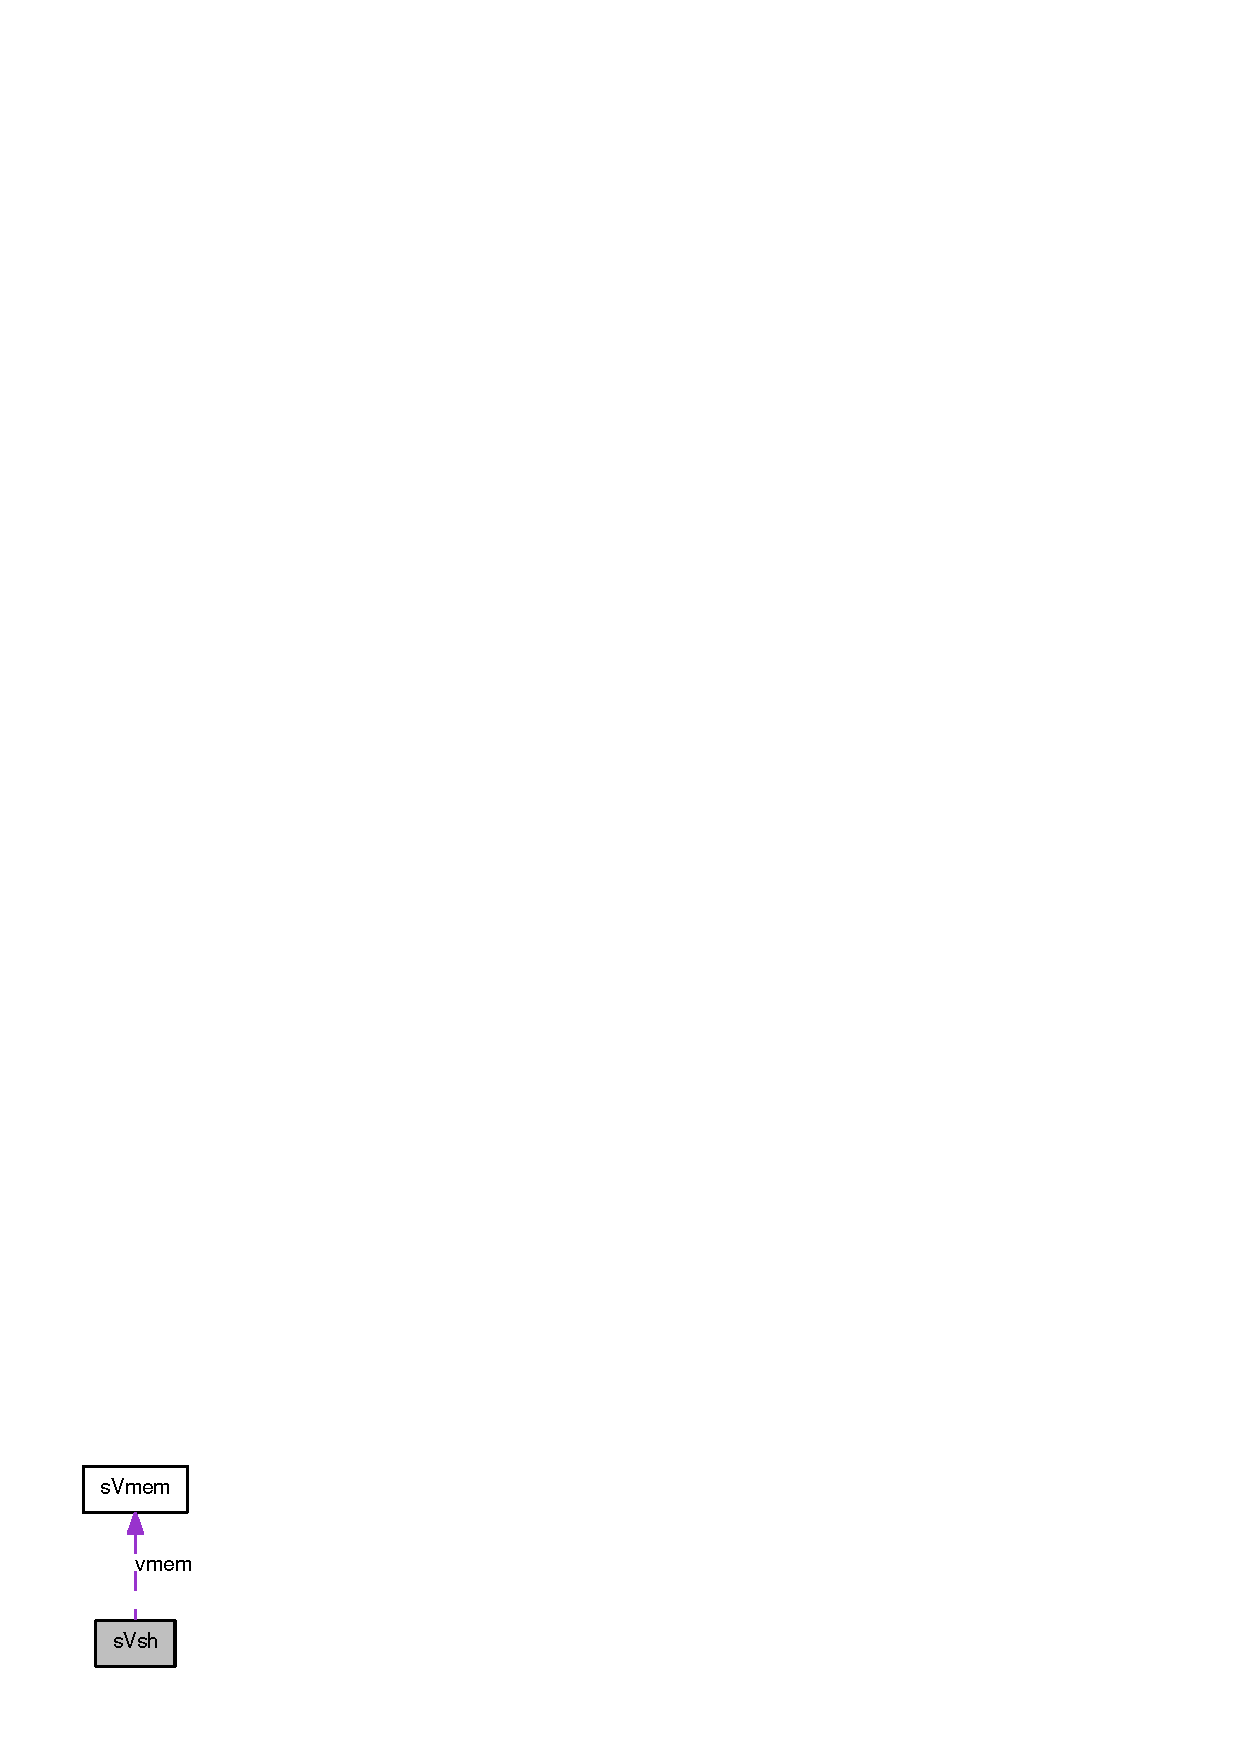
\includegraphics[width=96pt]{a00064}
\end{center}
\end{figure}
\subsection*{Public Attributes}
\begin{DoxyCompactItemize}
\item 
{\bf Vmem} $\ast$ {\bf vmem}
\begin{DoxyCompactList}\small\item\em the memory manager \item\end{DoxyCompactList}\item 
int {\bf iMadeVmem}
\begin{DoxyCompactList}\small\item\em did i make vmem or was it inherited \item\end{DoxyCompactList}\item 
char {\bf processArgs}
\begin{DoxyCompactList}\small\item\em whether the shell should process (argc,argv) \item\end{DoxyCompactList}\item 
int {\bf envValuLen}
\begin{DoxyCompactList}\small\item\em number of environment variables \item\end{DoxyCompactList}\item 
int {\bf envInfoLen}
\begin{DoxyCompactList}\small\item\em number of environment variable help strings \item\end{DoxyCompactList}\item 
char $\ast$$\ast$ {\bf envValu}
\begin{DoxyCompactList}\small\item\em the environment variables \item\end{DoxyCompactList}\item 
char $\ast$$\ast$ {\bf envInfo}
\begin{DoxyCompactList}\small\item\em the environment variable help strings \item\end{DoxyCompactList}\item 
FILE $\ast$ {\bf inUnit}
\begin{DoxyCompactList}\small\item\em input unit \item\end{DoxyCompactList}\item 
FILE $\ast$ {\bf scUnit}
\begin{DoxyCompactList}\small\item\em script input unit \item\end{DoxyCompactList}\item 
FILE $\ast$ {\bf clUnit}
\begin{DoxyCompactList}\small\item\em input unit \item\end{DoxyCompactList}\item 
FILE $\ast$ {\bf cinUnit}
\begin{DoxyCompactList}\small\item\em input unit \item\end{DoxyCompactList}\item 
char {\bf cinName} [VMAX\_\-ARGLEN]
\begin{DoxyCompactList}\small\item\em input unit \item\end{DoxyCompactList}\item 
char {\bf PR} [VMAX\_\-ARGLEN]
\begin{DoxyCompactList}\small\item\em minimal prompt (just the binary name) \item\end{DoxyCompactList}\item 
char {\bf PR\_\-PATH} [VMAX\_\-ARGLEN]
\begin{DoxyCompactList}\small\item\em full prompt (user,hostname,path,etc) \item\end{DoxyCompactList}\item 
char {\bf PR\_\-EXIT} [VMAX\_\-ARGLEN]
\begin{DoxyCompactList}\small\item\em the exit print string \item\end{DoxyCompactList}\item 
int {\bf cmdKey}
\begin{DoxyCompactList}\small\item\em external supershell command key \item\end{DoxyCompactList}\item 
void $\ast$ {\bf Ext\_\-thee}
\begin{DoxyCompactList}\small\item\em external supershell object \item\end{DoxyCompactList}\item 
char $\ast$ {\bf buf}
\begin{DoxyCompactList}\small\item\em internal buffer \item\end{DoxyCompactList}\item 
int {\bf bufsize}
\begin{DoxyCompactList}\small\item\em internal buffer size \item\end{DoxyCompactList}\item 
int($\ast$ {\bf Ext\_\-builtin} )(void $\ast$thee, int argc, char $\ast$$\ast$argv)
\begin{DoxyCompactList}\small\item\em external supershell builtin function \item\end{DoxyCompactList}\end{DoxyCompactItemize}


\subsection{Detailed Description}
Contains public data members for Vsh class. \begin{DoxyAuthor}{Author}
Michael Holst 
\end{DoxyAuthor}


\subsection{Member Data Documentation}
\index{sVsh@{sVsh}!buf@{buf}}
\index{buf@{buf}!sVsh@{sVsh}}
\subsubsection[{buf}]{\setlength{\rightskip}{0pt plus 5cm}char$\ast$ {\bf sVsh::buf}}\label{a00007_a54d6581a859ce3e568994a2acb34eeca}


internal buffer 

\index{sVsh@{sVsh}!bufsize@{bufsize}}
\index{bufsize@{bufsize}!sVsh@{sVsh}}
\subsubsection[{bufsize}]{\setlength{\rightskip}{0pt plus 5cm}int {\bf sVsh::bufsize}}\label{a00007_a3178ea2c169d30c7de2db923c6fc1472}


internal buffer size 

\index{sVsh@{sVsh}!cinName@{cinName}}
\index{cinName@{cinName}!sVsh@{sVsh}}
\subsubsection[{cinName}]{\setlength{\rightskip}{0pt plus 5cm}char {\bf sVsh::cinName}[VMAX\_\-ARGLEN]}\label{a00007_a4f656d4cfedad44dfa387f941aaf1f70}


input unit 

\index{sVsh@{sVsh}!cinUnit@{cinUnit}}
\index{cinUnit@{cinUnit}!sVsh@{sVsh}}
\subsubsection[{cinUnit}]{\setlength{\rightskip}{0pt plus 5cm}FILE$\ast$ {\bf sVsh::cinUnit}}\label{a00007_aafb169c1a906339713936d6434f1aab2}


input unit 

\index{sVsh@{sVsh}!clUnit@{clUnit}}
\index{clUnit@{clUnit}!sVsh@{sVsh}}
\subsubsection[{clUnit}]{\setlength{\rightskip}{0pt plus 5cm}FILE$\ast$ {\bf sVsh::clUnit}}\label{a00007_a61c33aa2071b43a85120b75d3984eeb3}


input unit 

\index{sVsh@{sVsh}!cmdKey@{cmdKey}}
\index{cmdKey@{cmdKey}!sVsh@{sVsh}}
\subsubsection[{cmdKey}]{\setlength{\rightskip}{0pt plus 5cm}int {\bf sVsh::cmdKey}}\label{a00007_aa246875bf82605333f30af61afe3ed54}


external supershell command key 

\index{sVsh@{sVsh}!envInfo@{envInfo}}
\index{envInfo@{envInfo}!sVsh@{sVsh}}
\subsubsection[{envInfo}]{\setlength{\rightskip}{0pt plus 5cm}char$\ast$$\ast$ {\bf sVsh::envInfo}}\label{a00007_a4b13b56b6059a20538b0eca39b1872b0}


the environment variable help strings 

\index{sVsh@{sVsh}!envInfoLen@{envInfoLen}}
\index{envInfoLen@{envInfoLen}!sVsh@{sVsh}}
\subsubsection[{envInfoLen}]{\setlength{\rightskip}{0pt plus 5cm}int {\bf sVsh::envInfoLen}}\label{a00007_a9f3e8263b78fe0574642e64ee6e30998}


number of environment variable help strings 

\index{sVsh@{sVsh}!envValu@{envValu}}
\index{envValu@{envValu}!sVsh@{sVsh}}
\subsubsection[{envValu}]{\setlength{\rightskip}{0pt plus 5cm}char$\ast$$\ast$ {\bf sVsh::envValu}}\label{a00007_a651413ef7fd726eef389669cff1f3e10}


the environment variables 

\index{sVsh@{sVsh}!envValuLen@{envValuLen}}
\index{envValuLen@{envValuLen}!sVsh@{sVsh}}
\subsubsection[{envValuLen}]{\setlength{\rightskip}{0pt plus 5cm}int {\bf sVsh::envValuLen}}\label{a00007_a6f5d3a3bfe8edef74e14262dca64eb19}


number of environment variables 

\index{sVsh@{sVsh}!Ext\_\-builtin@{Ext\_\-builtin}}
\index{Ext\_\-builtin@{Ext\_\-builtin}!sVsh@{sVsh}}
\subsubsection[{Ext\_\-builtin}]{\setlength{\rightskip}{0pt plus 5cm}int($\ast$ {\bf sVsh::Ext\_\-builtin})(void $\ast$thee, int argc, char $\ast$$\ast$argv)}\label{a00007_a1ede7298d7d963598ff09330b4dabf65}


external supershell builtin function 

\index{sVsh@{sVsh}!Ext\_\-thee@{Ext\_\-thee}}
\index{Ext\_\-thee@{Ext\_\-thee}!sVsh@{sVsh}}
\subsubsection[{Ext\_\-thee}]{\setlength{\rightskip}{0pt plus 5cm}void$\ast$ {\bf sVsh::Ext\_\-thee}}\label{a00007_aca365034a12a00d62f79aea0e74c24c0}


external supershell object 

\index{sVsh@{sVsh}!iMadeVmem@{iMadeVmem}}
\index{iMadeVmem@{iMadeVmem}!sVsh@{sVsh}}
\subsubsection[{iMadeVmem}]{\setlength{\rightskip}{0pt plus 5cm}int {\bf sVsh::iMadeVmem}}\label{a00007_a4d9333d357f6b00cb9d6a9152835385a}


did i make vmem or was it inherited 

\index{sVsh@{sVsh}!inUnit@{inUnit}}
\index{inUnit@{inUnit}!sVsh@{sVsh}}
\subsubsection[{inUnit}]{\setlength{\rightskip}{0pt plus 5cm}FILE$\ast$ {\bf sVsh::inUnit}}\label{a00007_a71b219a119b8ea2d6a8e8310fff87ad5}


input unit 

\index{sVsh@{sVsh}!PR@{PR}}
\index{PR@{PR}!sVsh@{sVsh}}
\subsubsection[{PR}]{\setlength{\rightskip}{0pt plus 5cm}char {\bf sVsh::PR}[VMAX\_\-ARGLEN]}\label{a00007_ad8d9d3a62f8a4a3cb4378aa58df6c976}


minimal prompt (just the binary name) 

\index{sVsh@{sVsh}!PR\_\-EXIT@{PR\_\-EXIT}}
\index{PR\_\-EXIT@{PR\_\-EXIT}!sVsh@{sVsh}}
\subsubsection[{PR\_\-EXIT}]{\setlength{\rightskip}{0pt plus 5cm}char {\bf sVsh::PR\_\-EXIT}[VMAX\_\-ARGLEN]}\label{a00007_a5973c822b71c353f131271631bbb43d0}


the exit print string 

\index{sVsh@{sVsh}!PR\_\-PATH@{PR\_\-PATH}}
\index{PR\_\-PATH@{PR\_\-PATH}!sVsh@{sVsh}}
\subsubsection[{PR\_\-PATH}]{\setlength{\rightskip}{0pt plus 5cm}char {\bf sVsh::PR\_\-PATH}[VMAX\_\-ARGLEN]}\label{a00007_a3d143e1a14f7ccd95292039d17679c17}


full prompt (user,hostname,path,etc) 

\index{sVsh@{sVsh}!processArgs@{processArgs}}
\index{processArgs@{processArgs}!sVsh@{sVsh}}
\subsubsection[{processArgs}]{\setlength{\rightskip}{0pt plus 5cm}char {\bf sVsh::processArgs}}\label{a00007_a4787c933c7915d6c1f8500e8d97abe7c}


whether the shell should process (argc,argv) 

\index{sVsh@{sVsh}!scUnit@{scUnit}}
\index{scUnit@{scUnit}!sVsh@{sVsh}}
\subsubsection[{scUnit}]{\setlength{\rightskip}{0pt plus 5cm}FILE$\ast$ {\bf sVsh::scUnit}}\label{a00007_a471927ccabdbbb75601d1d406e8cbc76}


script input unit 

\index{sVsh@{sVsh}!vmem@{vmem}}
\index{vmem@{vmem}!sVsh@{sVsh}}
\subsubsection[{vmem}]{\setlength{\rightskip}{0pt plus 5cm}{\bf Vmem}$\ast$ {\bf sVsh::vmem}}\label{a00007_a6ff199aeb0841047c1c4cd0a42f3c23a}


the memory manager 



The documentation for this struct was generated from the following file:\begin{DoxyCompactItemize}
\item 
{\bf vsh.h}\end{DoxyCompactItemize}

\chapter{File Documentation}
\section{license.h File Reference}
\label{a00008}\index{license.h@{license.h}}

\section{maloc.\+h File Reference}
\label{a00009}\index{maloc.\+h@{maloc.\+h}}


The foundation header for M\+A\+L\+O\+C.  


{\ttfamily \#include $<$maloc/maloc\+\_\+base.\+h$>$}\\*
{\ttfamily \#include $<$maloc/vsys.\+h$>$}\\*
{\ttfamily \#include $<$maloc/vsh.\+h$>$}\\*
{\ttfamily \#include $<$maloc/psh.\+h$>$}\\*
Include dependency graph for maloc.\+h\+:\nopagebreak
\begin{figure}[H]
\begin{center}
\leavevmode
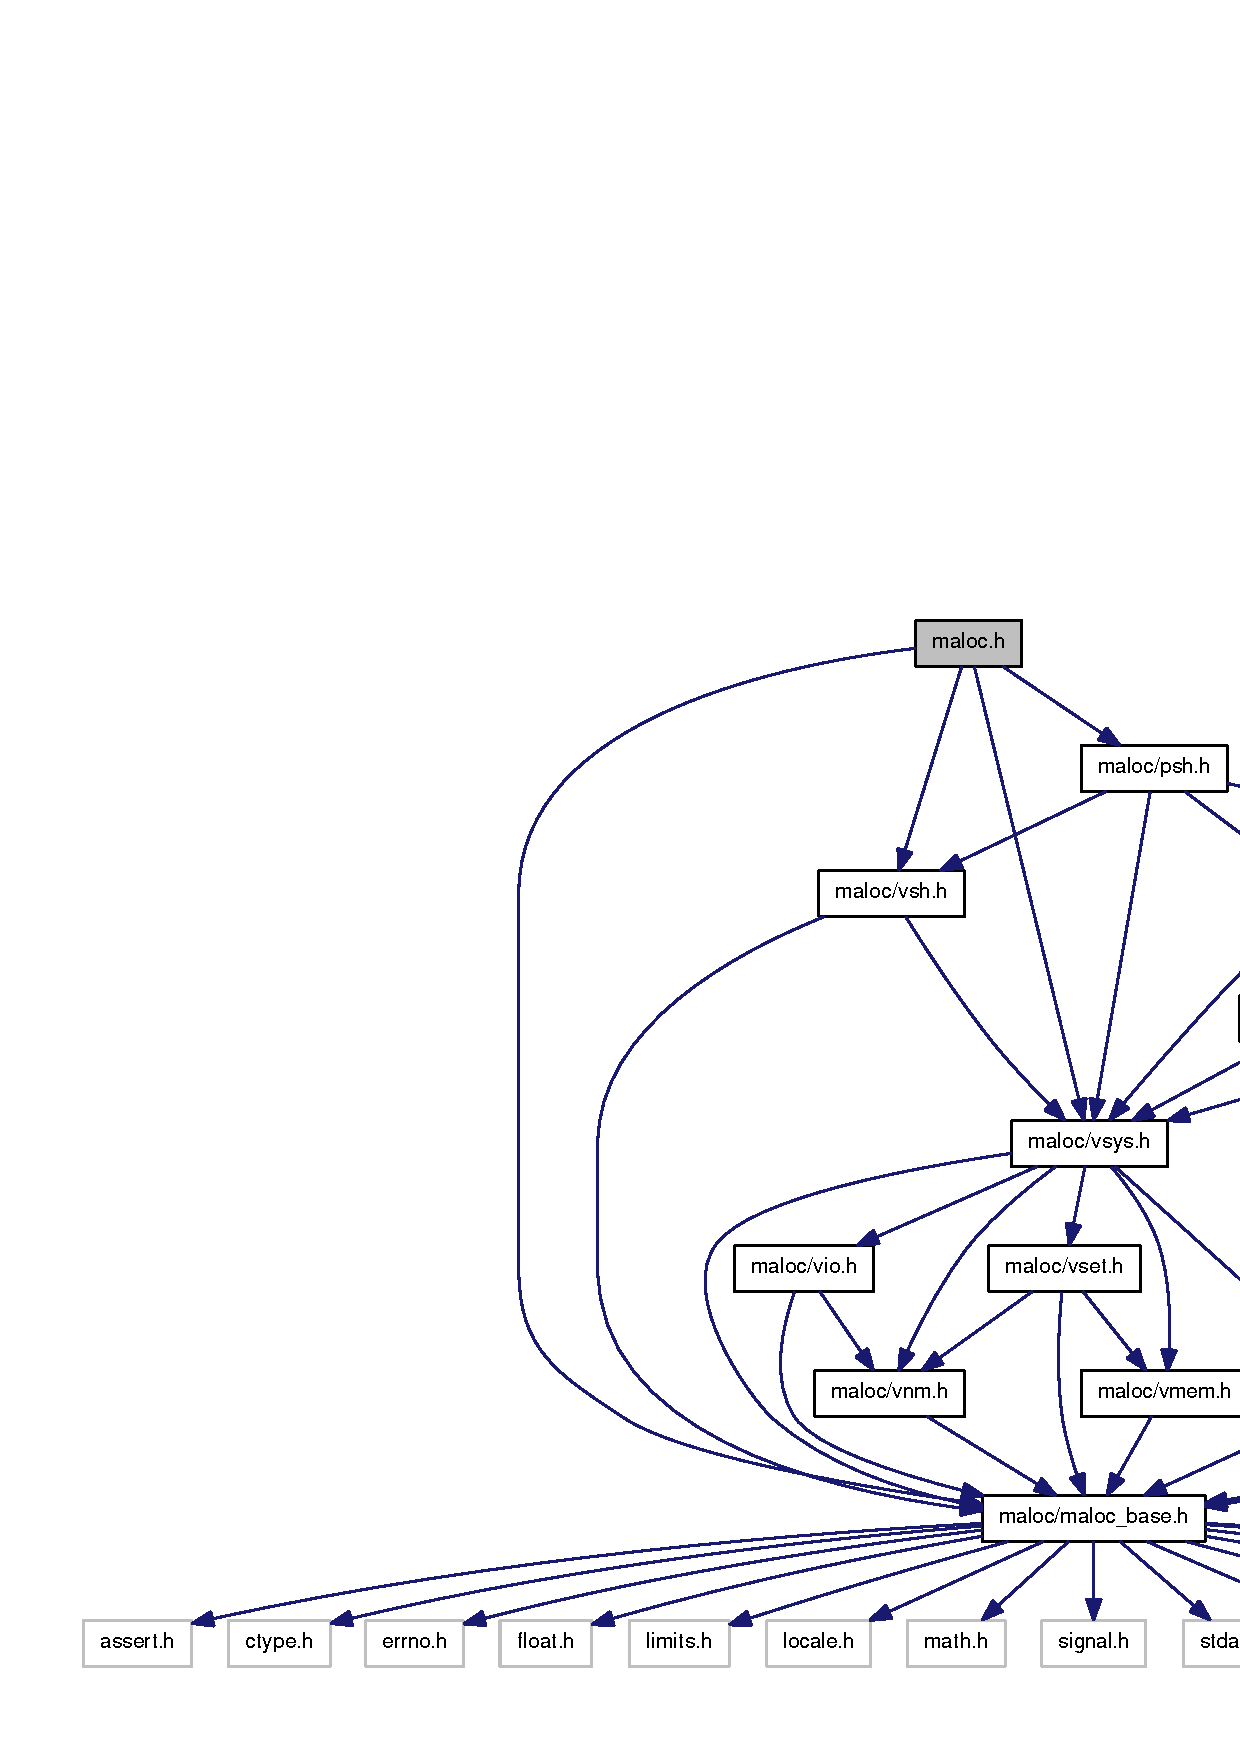
\includegraphics[width=350pt]{a00032}
\end{center}
\end{figure}


\subsection{Detailed Description}
The foundation header for M\+A\+L\+O\+C. 

\begin{DoxyAuthor}{Author}
Michael Holst 
\end{DoxyAuthor}
\begin{DoxyNote}{Note}
This is the main header file for all of M\+A\+L\+O\+C. This is the only file that needs to be included in order to access the entire library. 
\end{DoxyNote}
\begin{DoxyVersion}{Version}

\end{DoxyVersion}
\begin{DoxyParagraph}{Id}
\doxyref{maloc.\+h}{p.}{a00009},v 1.\+21 2010/08/12 05\+:40\+:13 fetk Exp 
\end{DoxyParagraph}


\begin{DoxyAttention}{Attention}
\begin{DoxyVerb}*
* MALOC = < Minimal Abstraction Layer for Object-oriented C >
* Copyright (C) 1994-- Michael Holst
*
* This library is free software; you can redistribute it and/or
* modify it under the terms of the GNU Lesser General Public
* License as published by the Free Software Foundation; either
* version 2.1 of the License, or (at your option) any later version.
*
* This library is distributed in the hope that it will be useful,
* but WITHOUT ANY WARRANTY; without even the implied warranty of
* MERCHANTABILITY or FITNESS FOR A PARTICULAR PURPOSE. See the GNU
* Lesser General Public License for more details.
*
* You should have received a copy of the GNU Lesser General Public
* License along with this library; if not, write to the Free Software
* Foundation, Inc., 59 Temple Place, Suite 330, Boston, MA 02111-1307 USA
* 
*  \end{DoxyVerb}
 
\end{DoxyAttention}

\section{maloc\_\-base.h File Reference}
\label{a00010}\index{maloc\_\-base.h@{maloc\_\-base.h}}


The base (or foundation) header for MALOC.  


{\ttfamily \#include $<$assert.h$>$}\par
{\ttfamily \#include $<$ctype.h$>$}\par
{\ttfamily \#include $<$errno.h$>$}\par
{\ttfamily \#include $<$float.h$>$}\par
{\ttfamily \#include $<$limits.h$>$}\par
{\ttfamily \#include $<$locale.h$>$}\par
{\ttfamily \#include $<$math.h$>$}\par
{\ttfamily \#include $<$signal.h$>$}\par
{\ttfamily \#include $<$stdarg.h$>$}\par
{\ttfamily \#include $<$stddef.h$>$}\par
{\ttfamily \#include $<$stdio.h$>$}\par
{\ttfamily \#include $<$stdlib.h$>$}\par
{\ttfamily \#include $<$string.h$>$}\par
{\ttfamily \#include $<$time.h$>$}\par
{\ttfamily \#include $<$setjmp.h$>$}\par
Include dependency graph for maloc\_\-base.h:
\nopagebreak
\begin{figure}[H]
\begin{center}
\leavevmode
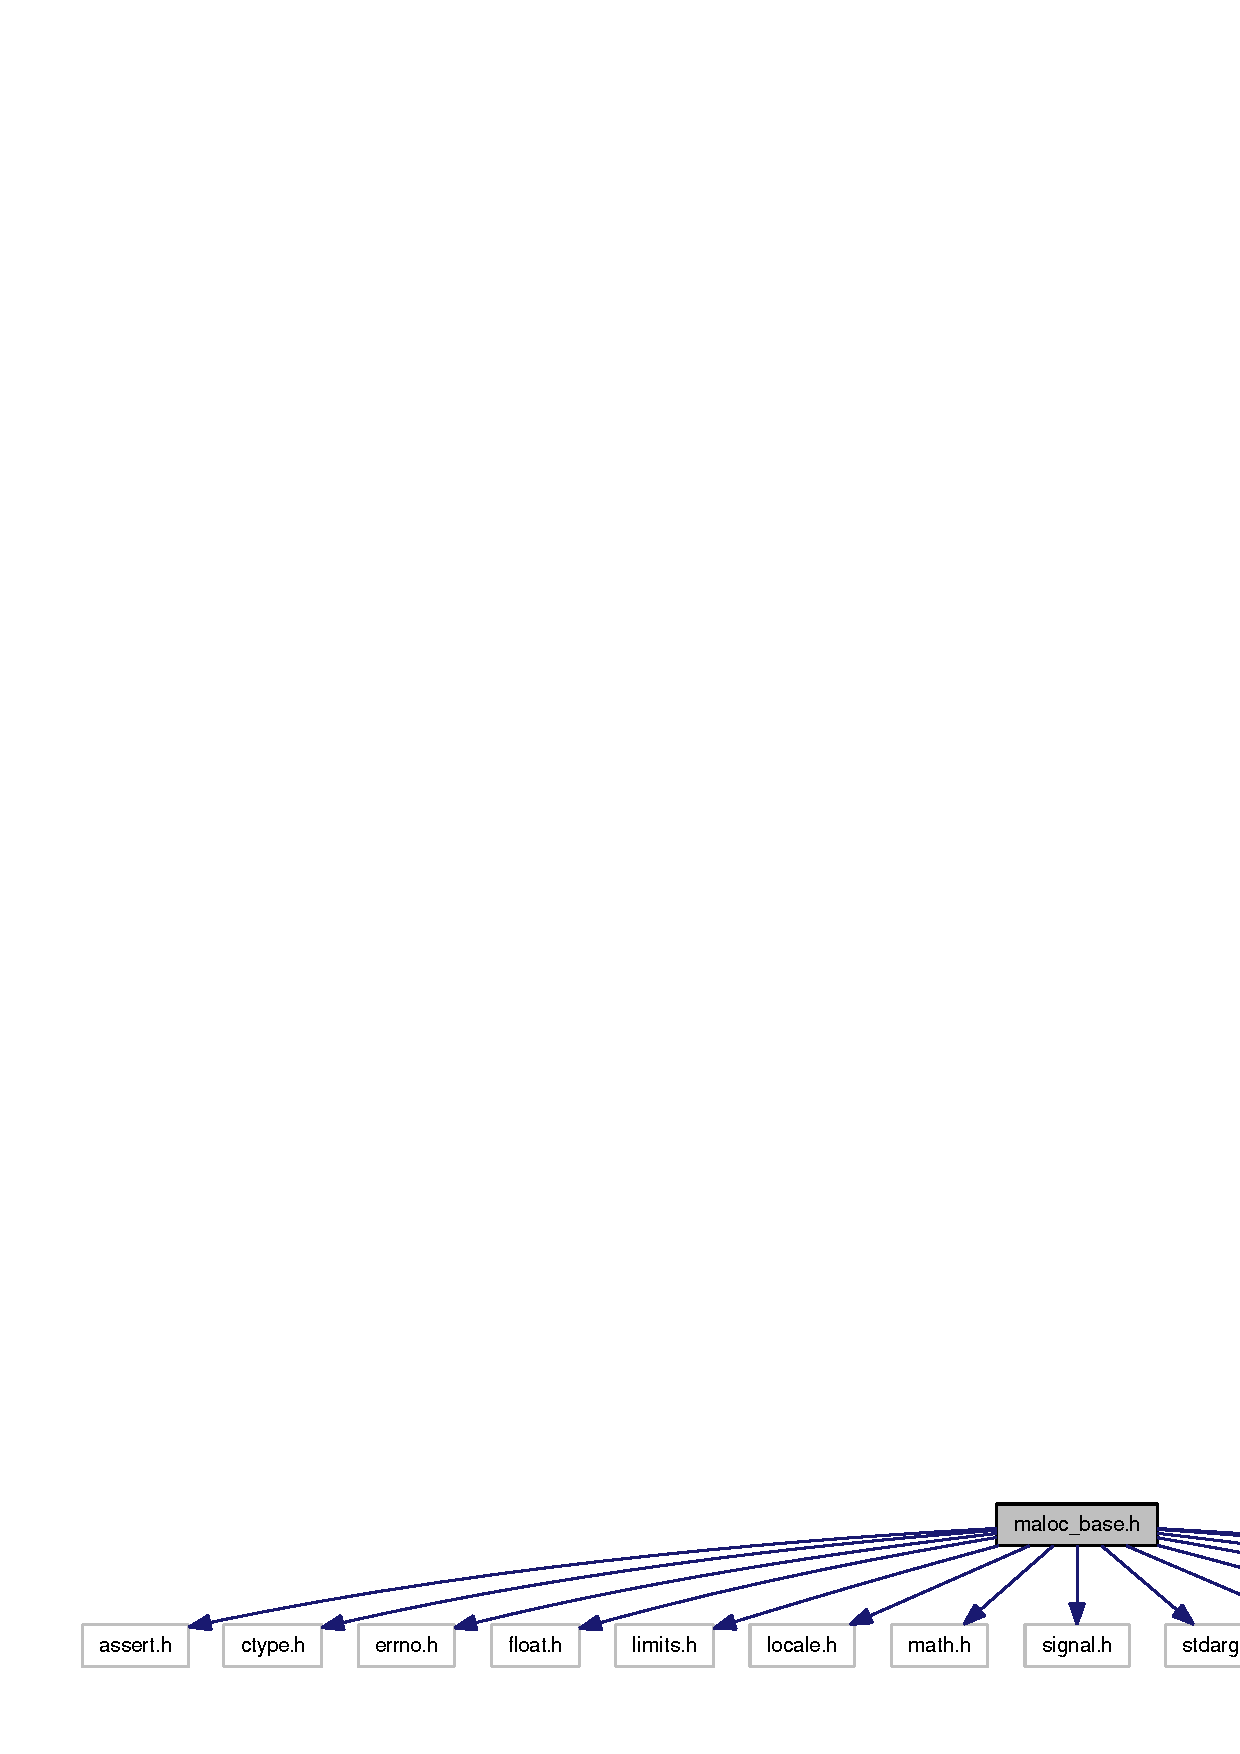
\includegraphics[width=400pt]{a00033}
\end{center}
\end{figure}
This graph shows which files directly or indirectly include this file:
\nopagebreak
\begin{figure}[H]
\begin{center}
\leavevmode
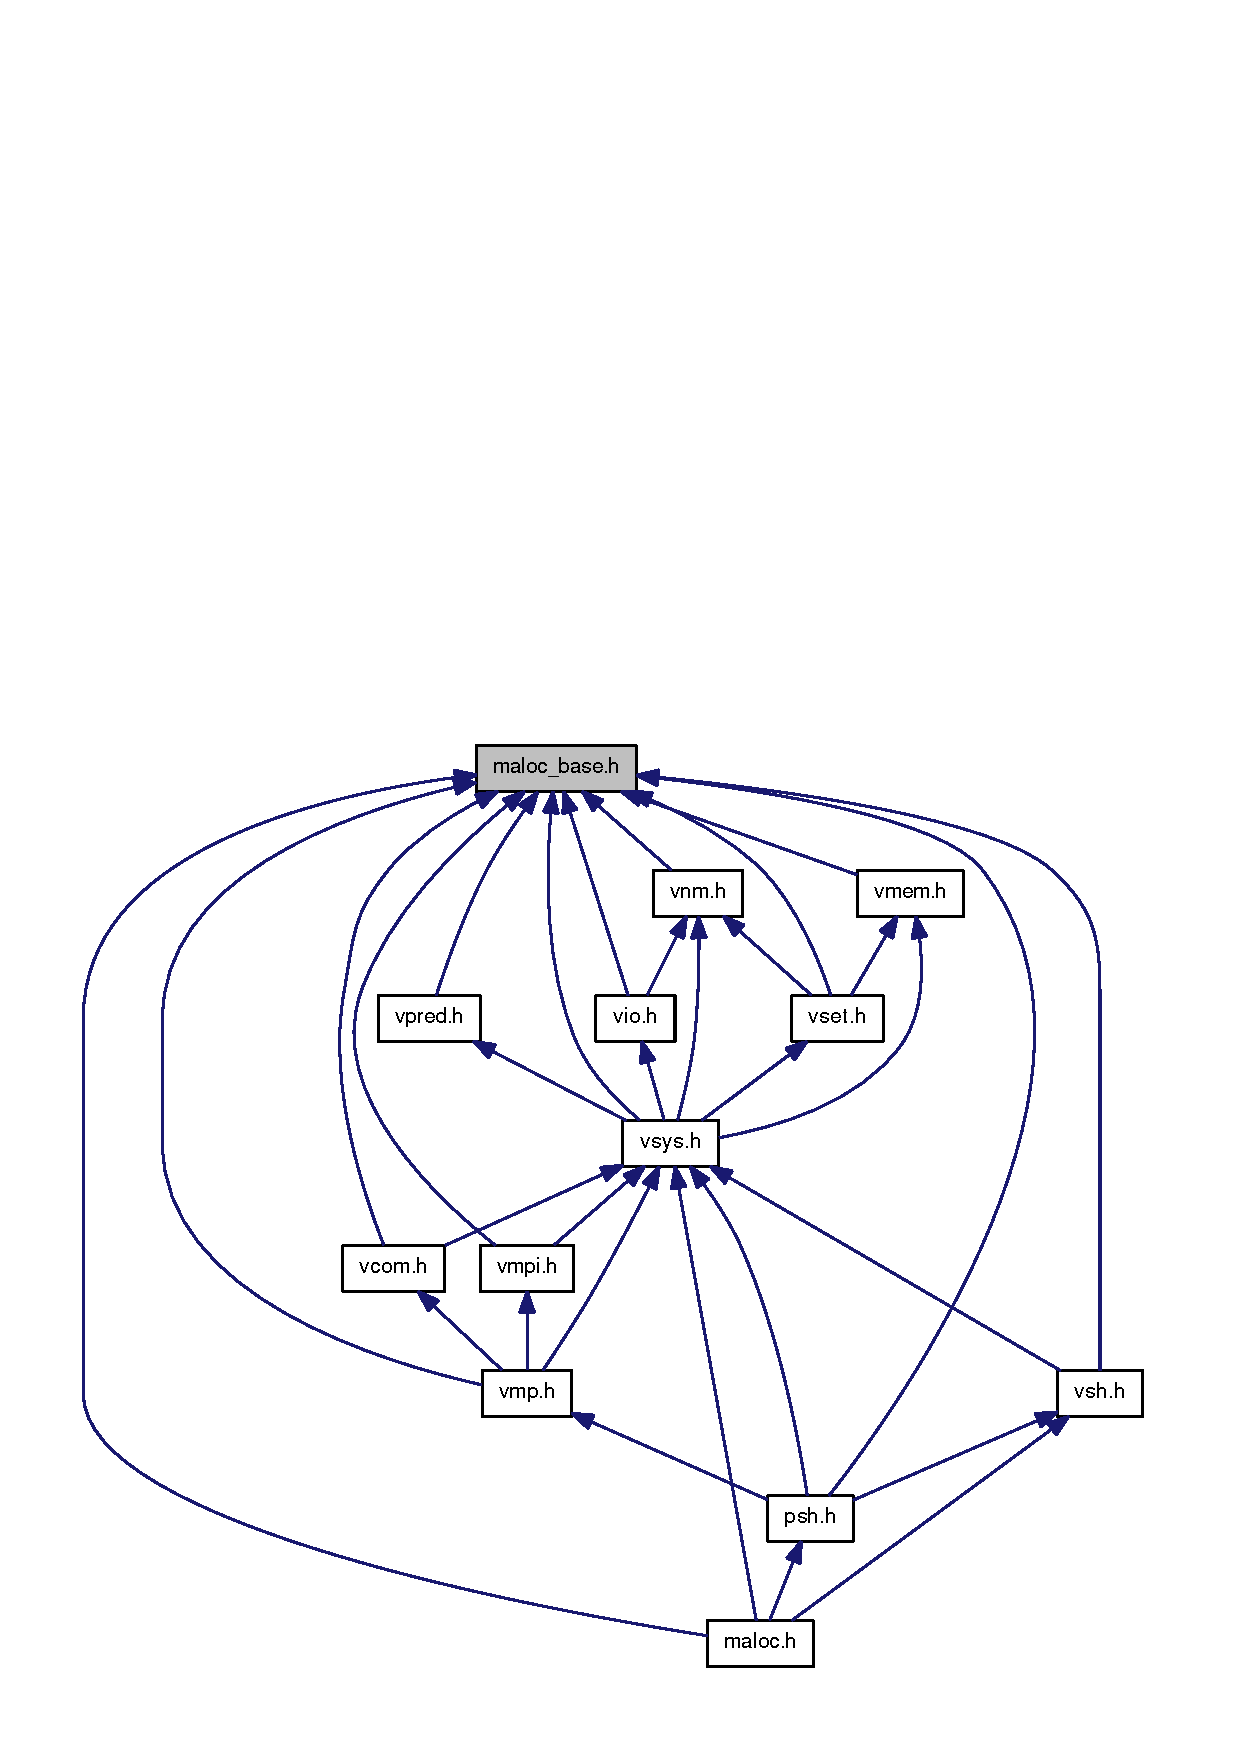
\includegraphics[width=400pt]{a00034}
\end{center}
\end{figure}
\subsection*{Defines}
\begin{DoxyCompactItemize}
\item 
\#define {\bf CLOCKS\_\-PER\_\-SEC}~60
\begin{DoxyCompactList}\small\item\em Fix to broken $<$time.h$>$ on old SunOS. \item\end{DoxyCompactList}\item 
\#define {\bf \_\-\_\-FAVOR\_\-BSD}
\begin{DoxyCompactList}\small\item\em Linux: uses sigsetjmp as the setjmp function. \item\end{DoxyCompactList}\item 
\#define {\bf \_\-BSD\_\-SIGNALS}
\begin{DoxyCompactList}\small\item\em IRIX: uses sigsetjmp as the setjmp function. \item\end{DoxyCompactList}\item 
\#define {\bf VCC}
\begin{DoxyCompactList}\small\item\em Setup so this include file (and subsequent) will work for both C and C++. \item\end{DoxyCompactList}\item 
\#define {\bf extern}
\begin{DoxyCompactList}\small\item\em Setup so this include file (and subsequent) will work for both C and C++. \item\end{DoxyCompactList}\item 
\#define {\bf VPRIVATE}~static
\begin{DoxyCompactList}\small\item\em Mimic C++ \char`\"{}Private\char`\"{} type modifier. \item\end{DoxyCompactList}\item 
\#define {\bf VPUBLIC}~/$\ast$empty$\ast$/
\begin{DoxyCompactList}\small\item\em Mimic C++ \char`\"{}Public\char`\"{} type modifier. \item\end{DoxyCompactList}\item 
\#define {\bf VWARN1}(file, lineno)~(fprintf(stderr,\char`\"{}VWARN: ASSERTION FAILURE! filename \%s, line \%u$\backslash$n\char`\"{}, (file), (lineno)), 0)
\begin{DoxyCompactList}\small\item\em Slick assertion macro. \item\end{DoxyCompactList}\item 
\#define {\bf VASSERT1}(file, lineno)~(fprintf(stderr,\char`\"{}VASSERT: ASSERTION FAILURE! filename \%s, line \%u$\backslash$n\char`\"{}, (file), (lineno)), exit(1), 0)
\begin{DoxyCompactList}\small\item\em Slick assertion macro. \item\end{DoxyCompactList}\item 
\#define {\bf VASSERT2}(file, lineno)~(fprintf(stderr,\char`\"{}VASSERT: ASSERTION FAILURE! filename \%s, line \%u$\backslash$n\char`\"{}, (file), (lineno)), abort(), 0)
\begin{DoxyCompactList}\small\item\em Slick assertion macro. \item\end{DoxyCompactList}\item 
\#define {\bf VASSERT3}(file, lineno, ex)~(fprintf(stderr,\char`\"{}VASSERT: ASSERTION FAILURE!  filename \%s, line \%u, (\%s)$\backslash$n\char`\"{}, (file), (lineno), (\#ex)), abort(), 0)
\begin{DoxyCompactList}\small\item\em Slick assertion macro. \item\end{DoxyCompactList}\item 
\#define {\bf VWARN}(ex)~((void) ((ex) ? 0 : VWARN1(\_\-\_\-FILE\_\-\_\-, \_\-\_\-LINE\_\-\_\-)))
\begin{DoxyCompactList}\small\item\em Slick assertion macro. \item\end{DoxyCompactList}\item 
\#define {\bf VASSERT}(ex)~((void) ((ex) ? 0 : VASSERT3(\_\-\_\-FILE\_\-\_\-, \_\-\_\-LINE\_\-\_\-, ex)))
\begin{DoxyCompactList}\small\item\em Slick assertion macro. \item\end{DoxyCompactList}\item 
\#define {\bf VJMPERR0}(x)~if (!(x)) goto VERROR0
\begin{DoxyCompactList}\small\item\em A userful error handling macro. \item\end{DoxyCompactList}\item 
\#define {\bf VJMPERR1}(x)~if (!(x)) goto VERROR1
\begin{DoxyCompactList}\small\item\em A userful error handling macro. \item\end{DoxyCompactList}\item 
\#define {\bf VJMPERR2}(x)~if (!(x)) goto VERROR2
\begin{DoxyCompactList}\small\item\em A userful error handling macro. \item\end{DoxyCompactList}\item 
\#define {\bf VJMPERR3}(x)~if (!(x)) goto VERROR3
\begin{DoxyCompactList}\small\item\em A userful error handling macro. \item\end{DoxyCompactList}\item 
\#define {\bf VJMPERR4}(x)~if (!(x)) goto VERROR4
\begin{DoxyCompactList}\small\item\em A userful error handling macro. \item\end{DoxyCompactList}\item 
\#define {\bf VJMPERR5}(x)~if (!(x)) goto VERROR5
\begin{DoxyCompactList}\small\item\em A userful error handling macro. \item\end{DoxyCompactList}\item 
\#define {\bf VJMPERR6}(x)~if (!(x)) goto VERROR6
\begin{DoxyCompactList}\small\item\em A userful error handling macro. \item\end{DoxyCompactList}\item 
\#define {\bf VJMPERR7}(x)~if (!(x)) goto VERROR7
\begin{DoxyCompactList}\small\item\em A userful error handling macro. \item\end{DoxyCompactList}\item 
\#define {\bf VJMPERR8}(x)~if (!(x)) goto VERROR8
\begin{DoxyCompactList}\small\item\em A userful error handling macro. \item\end{DoxyCompactList}\item 
\#define {\bf VJMPERR9}(x)~if (!(x)) goto VERROR9
\begin{DoxyCompactList}\small\item\em A userful error handling macro. \item\end{DoxyCompactList}\item 
\#define {\bf VPI}~3.14159265358979323846
\begin{DoxyCompactList}\small\item\em Global constant. \item\end{DoxyCompactList}\item 
\#define {\bf VLARGE}~1.0e+9
\begin{DoxyCompactList}\small\item\em Global constant. 1e9 just fits into 32-\/bit signed int. \item\end{DoxyCompactList}\item 
\#define {\bf VSMALL}~1.0e-\/9
\begin{DoxyCompactList}\small\item\em Global constant. \item\end{DoxyCompactList}\item 
\#define {\bf VVLARGE}~1.0e+15
\begin{DoxyCompactList}\small\item\em Global constant. \item\end{DoxyCompactList}\item 
\#define {\bf VVSMALL}~1.0e-\/15
\begin{DoxyCompactList}\small\item\em Global constant. \item\end{DoxyCompactList}\item 
\#define {\bf VPRTKEY}~10000
\begin{DoxyCompactList}\small\item\em Global constant. \item\end{DoxyCompactList}\item 
\#define {\bf VPTRSIZE}~4
\begin{DoxyCompactList}\small\item\em Global constant. \item\end{DoxyCompactList}\item 
\#define {\bf VMAX\_\-ARGNUM}~50
\begin{DoxyCompactList}\small\item\em Global constant. \item\end{DoxyCompactList}\item 
\#define {\bf VMAX\_\-ARGLEN}~1024
\begin{DoxyCompactList}\small\item\em Global constant. \item\end{DoxyCompactList}\item 
\#define {\bf VMAX\_\-BUFSIZE}~8192
\begin{DoxyCompactList}\small\item\em Global constant. \item\end{DoxyCompactList}\item 
\#define {\bf VMAX\_\-OBJECTS}~1073741824
\begin{DoxyCompactList}\small\item\em Global constant. \item\end{DoxyCompactList}\item 
\#define {\bf VBLOCK\_\-POWER}~14
\begin{DoxyCompactList}\small\item\em Global constant. \item\end{DoxyCompactList}\item 
\#define {\bf VNULL}~NULL
\begin{DoxyCompactList}\small\item\em Global constant. \item\end{DoxyCompactList}\item 
\#define {\bf VINULL}~-\/1
\begin{DoxyCompactList}\small\item\em Global constant. \item\end{DoxyCompactList}\item 
\#define {\bf VTRUE}~1
\begin{DoxyCompactList}\small\item\em Global constant. \item\end{DoxyCompactList}\item 
\#define {\bf VFALSE}~0
\begin{DoxyCompactList}\small\item\em Global constant. \item\end{DoxyCompactList}\item 
\#define {\bf VSTDMODE}~0600
\begin{DoxyCompactList}\small\item\em Global constant. \item\end{DoxyCompactList}\item 
\#define {\bf VNULL\_\-STRING}~\char`\"{}$\backslash$0\char`\"{}
\begin{DoxyCompactList}\small\item\em Global constant. \item\end{DoxyCompactList}\item 
\#define {\bf VBLANK\_\-STRING}~\char`\"{} \char`\"{}
\begin{DoxyCompactList}\small\item\em Global constant. \item\end{DoxyCompactList}\item 
\#define {\bf VNEWLINE\_\-STRING}~\char`\"{}$\backslash$n\char`\"{}
\begin{DoxyCompactList}\small\item\em Global constant. \item\end{DoxyCompactList}\item 
\#define {\bf VNULL\_\-SYMBOL}~'$\backslash$0'
\begin{DoxyCompactList}\small\item\em Global constant. \item\end{DoxyCompactList}\item 
\#define {\bf VBLANK\_\-SYMBOL}~' '
\begin{DoxyCompactList}\small\item\em Global constant. \item\end{DoxyCompactList}\item 
\#define {\bf VNEWLINE\_\-SYMBOL}~'$\backslash$n'
\begin{DoxyCompactList}\small\item\em Global constant. \item\end{DoxyCompactList}\item 
\#define {\bf VRDIN\_\-SYMBOL}~'$<$'
\begin{DoxyCompactList}\small\item\em Global constant. \item\end{DoxyCompactList}\item 
\#define {\bf VRDOUT\_\-SYMBOL}~'$>$'
\begin{DoxyCompactList}\small\item\em Global constant. \item\end{DoxyCompactList}\item 
\#define {\bf VPIPE\_\-SYMBOL}~'$|$'
\begin{DoxyCompactList}\small\item\em Global constant. \item\end{DoxyCompactList}\item 
\#define {\bf VDELIM\_\-SET}~\char`\"{} $>$$<$$|$\&\char`\"{}
\begin{DoxyCompactList}\small\item\em Global constant. \item\end{DoxyCompactList}\item 
\#define {\bf VABS}(x)~((x) $>$= 0 ? (x) : -\/(x))
\begin{DoxyCompactList}\small\item\em Mathematical macro. \item\end{DoxyCompactList}\item 
\#define {\bf VMIN2}(x, y)~((x) $<$= (y) ? (x) : (y))
\begin{DoxyCompactList}\small\item\em Mathematical macro. \item\end{DoxyCompactList}\item 
\#define {\bf VMAX2}(x, y)~((x) $>$= (y) ? (x) : (y))
\begin{DoxyCompactList}\small\item\em Mathematical macro. \item\end{DoxyCompactList}\item 
\#define {\bf VSIGN}(x, y)~((y) $>$= 0 ? (VABS(x)) : (-\/VABS(x)))
\begin{DoxyCompactList}\small\item\em Mathematical macro. \item\end{DoxyCompactList}\item 
\#define {\bf VODD}(x)~((x)\&1)
\begin{DoxyCompactList}\small\item\em Mathematical macro. \item\end{DoxyCompactList}\item 
\#define {\bf VEVEN}(x)~(!((x)\&1))
\begin{DoxyCompactList}\small\item\em Mathematical macro. \item\end{DoxyCompactList}\item 
\#define {\bf VZERO}(x)~((x)==0)
\begin{DoxyCompactList}\small\item\em Mathematical macro. \item\end{DoxyCompactList}\item 
\#define {\bf VPOS}(x)~((x)$>$0)
\begin{DoxyCompactList}\small\item\em Mathematical macro. \item\end{DoxyCompactList}\item 
\#define {\bf VNEG}(x)~((x)$<$0)
\begin{DoxyCompactList}\small\item\em Mathematical macro. \item\end{DoxyCompactList}\item 
\#define {\bf VEVENP}(x)~(VEVEN(x) \&\& VPOS(x))
\begin{DoxyCompactList}\small\item\em Mathematical macro. \item\end{DoxyCompactList}\item 
\#define {\bf VEVENN}(x)~(VEVEN(x) \&\& VNEG(x))
\begin{DoxyCompactList}\small\item\em Mathematical macro. \item\end{DoxyCompactList}\item 
\#define {\bf VSQRT}(x)~(sqrt(x))
\begin{DoxyCompactList}\small\item\em Mathematical macro. \item\end{DoxyCompactList}\item 
\#define {\bf VSQR}(x)~((x)$\ast$(x))
\begin{DoxyCompactList}\small\item\em Mathematical macro. \item\end{DoxyCompactList}\item 
\#define {\bf VSIN}(x)~(sin(x))
\begin{DoxyCompactList}\small\item\em Mathematical macro. \item\end{DoxyCompactList}\item 
\#define {\bf VCOS}(x)~(cos(x))
\begin{DoxyCompactList}\small\item\em Mathematical macro. \item\end{DoxyCompactList}\item 
\#define {\bf VTAN}(x)~(tan(x))
\begin{DoxyCompactList}\small\item\em Mathematical macro. \item\end{DoxyCompactList}\item 
\#define {\bf VASIN}(x)~(asin(x))
\begin{DoxyCompactList}\small\item\em Mathematical macro. \item\end{DoxyCompactList}\item 
\#define {\bf VACOS}(x)~(acos(x))
\begin{DoxyCompactList}\small\item\em Mathematical macro. \item\end{DoxyCompactList}\item 
\#define {\bf VATAN}(x)~(atan(x))
\begin{DoxyCompactList}\small\item\em Mathematical macro. \item\end{DoxyCompactList}\item 
\#define {\bf VSINH}(x)~(sinh(x))
\begin{DoxyCompactList}\small\item\em Mathematical macro. \item\end{DoxyCompactList}\item 
\#define {\bf VCOSH}(x)~(cosh(x))
\begin{DoxyCompactList}\small\item\em Mathematical macro. \item\end{DoxyCompactList}\item 
\#define {\bf VTANH}(x)~(tanh(x))
\begin{DoxyCompactList}\small\item\em Mathematical macro. \item\end{DoxyCompactList}\item 
\#define {\bf VEXP}(x)~(exp(x))
\begin{DoxyCompactList}\small\item\em Mathematical macro. \item\end{DoxyCompactList}\item 
\#define {\bf VLOG}(x)~(log(x))
\begin{DoxyCompactList}\small\item\em Mathematical macro. \item\end{DoxyCompactList}\item 
\#define {\bf VPOW}(x, y)~(pow(x,y))
\begin{DoxyCompactList}\small\item\em Mathematical macro. \item\end{DoxyCompactList}\item 
\#define {\bf VRINT}(x)~((int)(floor((x)+0.5)))
\begin{DoxyCompactList}\small\item\em Mathematical macro. \item\end{DoxyCompactList}\item 
\#define {\bf VRAND}~(rand())
\begin{DoxyCompactList}\small\item\em Mathematical macro. \item\end{DoxyCompactList}\item 
\#define {\bf VRANDMAX}~(RAND\_\-MAX)
\begin{DoxyCompactList}\small\item\em Mathematical macro. \item\end{DoxyCompactList}\item 
\#define {\bf VINLINE\_\-MALOC}
\begin{DoxyCompactList}\small\item\em Inlining via macros for speed. \item\end{DoxyCompactList}\end{DoxyCompactItemize}


\subsection{Detailed Description}
The base (or foundation) header for MALOC. \begin{DoxyAuthor}{Author}
Michael Holst 
\end{DoxyAuthor}
\begin{DoxyNote}{Note}
This header sets things up correctly for using ISO/ANSI-\/C. The following macros affect the behavior of the header: \begin{DoxyVerb}
     Inlining for speed:  (Normal C functions if VINLINE_XXX not defined.)    
     ------------------
     -DVINLINE_VNM : Enables macro replacement of time-critical funcs in VNM.
    \end{DoxyVerb}

\end{DoxyNote}
\begin{DoxyVersion}{Version}

\end{DoxyVersion}
\begin{DoxyParagraph}{Id:}
\doxyref{maloc\_\-base.h}{p.}{a00010},v 1.33 2010/08/12 05:40:16 fetk Exp 
\end{DoxyParagraph}


\begin{DoxyAttention}{Attention}
\begin{DoxyVerb}
 *
 * MALOC = < Minimal Abstraction Layer for Object-oriented C >
 * Copyright (C) 1994-- Michael Holst
 *
 * This library is free software; you can redistribute it and/or
 * modify it under the terms of the GNU Lesser General Public
 * License as published by the Free Software Foundation; either
 * version 2.1 of the License, or (at your option) any later version.
 *
 * This library is distributed in the hope that it will be useful,
 * but WITHOUT ANY WARRANTY; without even the implied warranty of
 * MERCHANTABILITY or FITNESS FOR A PARTICULAR PURPOSE. See the GNU
 * Lesser General Public License for more details.
 *
 * You should have received a copy of the GNU Lesser General Public
 * License along with this library; if not, write to the Free Software
 * Foundation, Inc., 59 Temple Place, Suite 330, Boston, MA 02111-1307 USA
 * 
 *  \end{DoxyVerb}
 
\end{DoxyAttention}


\subsection{Define Documentation}
\index{maloc\_\-base.h@{maloc\_\-base.h}!\_\-\_\-FAVOR\_\-BSD@{\_\-\_\-FAVOR\_\-BSD}}
\index{\_\-\_\-FAVOR\_\-BSD@{\_\-\_\-FAVOR\_\-BSD}!maloc_base.h@{maloc\_\-base.h}}
\subsubsection[{\_\-\_\-FAVOR\_\-BSD}]{\setlength{\rightskip}{0pt plus 5cm}\#define \_\-\_\-FAVOR\_\-BSD}\label{a00010_a0e25ec3d9c374c5e6dceeb9341baf766}


Linux: uses sigsetjmp as the setjmp function. 

\begin{DoxyNote}{Note}
\begin{DoxyVerb}
 * Problems using setjmp/longjmp for use in the MC-shell.
 *
 * Problem:  Some implementations of ISO-C "setjmp/longjmp"  do not return
 *           the interrupt mask to its pre-jump state after returning.
 *           The behavior this produces is for example you can capture a
 *           single CTRL-C, but that is it; the mask for CTRL-C is wiped
 *           after the first interrupt is handled.
 *
 * Solution: Use the "sigsetjmp/siglongjmp" extensions provided by most
 *           UNIX variants.  You just have to set an appropriate macro
 *           before including <setjmp.h> to get sigsetjmp rather than
 *           setjmp behavior.
 *
 * Notes:    You can run into trouble (e.g. some versions of Linux) if
 *           you set some of these special signal macros before some of
 *           the other ISO-C headers.  Therefore, we only set the macros
 *           just before including <setjmp.h> as the final ISO-C header.
 * \end{DoxyVerb}
 
\end{DoxyNote}
\index{maloc\_\-base.h@{maloc\_\-base.h}!\_\-BSD\_\-SIGNALS@{\_\-BSD\_\-SIGNALS}}
\index{\_\-BSD\_\-SIGNALS@{\_\-BSD\_\-SIGNALS}!maloc_base.h@{maloc\_\-base.h}}
\subsubsection[{\_\-BSD\_\-SIGNALS}]{\setlength{\rightskip}{0pt plus 5cm}\#define \_\-BSD\_\-SIGNALS}\label{a00010_a0efe403ab8687e820c8b6ea5a275d1a9}


IRIX: uses sigsetjmp as the setjmp function. 

\begin{DoxyNote}{Note}
\begin{DoxyVerb}
 * Problems using setjmp/longjmp for use in the MC-shell.
 *
 * Problem:  Some implementations of ISO-C "setjmp/longjmp"  do not return
 *           the interrupt mask to its pre-jump state after returning.
 *           The behavior this produces is for example you can capture a
 *           single CTRL-C, but that is it; the mask for CTRL-C is wiped
 *           after the first interrupt is handled.
 *
 * Solution: Use the "sigsetjmp/siglongjmp" extensions provided by most
 *           UNIX variants.  You just have to set an appropriate macro
 *           before including <setjmp.h> to get sigsetjmp rather than
 *           setjmp behavior.
 *
 * Notes:    You can run into trouble (e.g. some versions of Linux) if
 *           you set some of these special signal macros before some of
 *           the other ISO-C headers.  Therefore, we only set the macros
 *           just before including <setjmp.h> as the final ISO-C header.
 * \end{DoxyVerb}
 
\end{DoxyNote}
\index{maloc\_\-base.h@{maloc\_\-base.h}!CLOCKS\_\-PER\_\-SEC@{CLOCKS\_\-PER\_\-SEC}}
\index{CLOCKS\_\-PER\_\-SEC@{CLOCKS\_\-PER\_\-SEC}!maloc_base.h@{maloc\_\-base.h}}
\subsubsection[{CLOCKS\_\-PER\_\-SEC}]{\setlength{\rightskip}{0pt plus 5cm}\#define CLOCKS\_\-PER\_\-SEC~60}\label{a00010_a3d9fc3c745d0880902fe3ea3d5d5f71e}


Fix to broken $<$time.h$>$ on old SunOS. 

\index{maloc\_\-base.h@{maloc\_\-base.h}!extern@{extern}}
\index{extern@{extern}!maloc_base.h@{maloc\_\-base.h}}
\subsubsection[{extern}]{\setlength{\rightskip}{0pt plus 5cm}\#define extern}\label{a00010_a2a624a765564411c0db3a2bee940f8bc}


Setup so this include file (and subsequent) will work for both C and C++. 

\index{maloc\_\-base.h@{maloc\_\-base.h}!VABS@{VABS}}
\index{VABS@{VABS}!maloc_base.h@{maloc\_\-base.h}}
\subsubsection[{VABS}]{\setlength{\rightskip}{0pt plus 5cm}\#define VABS(
\begin{DoxyParamCaption}
\item[{}]{x}
\end{DoxyParamCaption}
)~((x) $>$= 0 ? (x) : -\/(x))}\label{a00010_a6a6283ab8af6569d4955242614b9427b}


Mathematical macro. 

\index{maloc\_\-base.h@{maloc\_\-base.h}!VACOS@{VACOS}}
\index{VACOS@{VACOS}!maloc_base.h@{maloc\_\-base.h}}
\subsubsection[{VACOS}]{\setlength{\rightskip}{0pt plus 5cm}\#define VACOS(
\begin{DoxyParamCaption}
\item[{}]{x}
\end{DoxyParamCaption}
)~(acos(x))}\label{a00010_a22bce1388a2c9218ef6c2bfd273e85cf}


Mathematical macro. 

\index{maloc\_\-base.h@{maloc\_\-base.h}!VASIN@{VASIN}}
\index{VASIN@{VASIN}!maloc_base.h@{maloc\_\-base.h}}
\subsubsection[{VASIN}]{\setlength{\rightskip}{0pt plus 5cm}\#define VASIN(
\begin{DoxyParamCaption}
\item[{}]{x}
\end{DoxyParamCaption}
)~(asin(x))}\label{a00010_ad87fe9fd002acdb16535b579510ddd44}


Mathematical macro. 

\index{maloc\_\-base.h@{maloc\_\-base.h}!VASSERT@{VASSERT}}
\index{VASSERT@{VASSERT}!maloc_base.h@{maloc\_\-base.h}}
\subsubsection[{VASSERT}]{\setlength{\rightskip}{0pt plus 5cm}\#define VASSERT(
\begin{DoxyParamCaption}
\item[{}]{ex}
\end{DoxyParamCaption}
)~((void) ((ex) ? 0 : VASSERT3(\_\-\_\-FILE\_\-\_\-, \_\-\_\-LINE\_\-\_\-, ex)))}\label{a00010_a0e080eee9e9eefed6f35db9fa4609e6a}


Slick assertion macro. 

\index{maloc\_\-base.h@{maloc\_\-base.h}!VASSERT1@{VASSERT1}}
\index{VASSERT1@{VASSERT1}!maloc_base.h@{maloc\_\-base.h}}
\subsubsection[{VASSERT1}]{\setlength{\rightskip}{0pt plus 5cm}\#define VASSERT1(
\begin{DoxyParamCaption}
\item[{}]{file, }
\item[{}]{lineno}
\end{DoxyParamCaption}
)~(fprintf(stderr,\char`\"{}VASSERT: ASSERTION FAILURE! filename \%s, line \%u$\backslash$n\char`\"{}, (file), (lineno)), exit(1), 0)}\label{a00010_a7944addb8188e6853c788d9a9e4fffe1}


Slick assertion macro. 

\index{maloc\_\-base.h@{maloc\_\-base.h}!VASSERT2@{VASSERT2}}
\index{VASSERT2@{VASSERT2}!maloc_base.h@{maloc\_\-base.h}}
\subsubsection[{VASSERT2}]{\setlength{\rightskip}{0pt plus 5cm}\#define VASSERT2(
\begin{DoxyParamCaption}
\item[{}]{file, }
\item[{}]{lineno}
\end{DoxyParamCaption}
)~(fprintf(stderr,\char`\"{}VASSERT: ASSERTION FAILURE! filename \%s, line \%u$\backslash$n\char`\"{}, (file), (lineno)), abort(), 0)}\label{a00010_a560710e925cc860ac762681c5bca74ce}


Slick assertion macro. 

\index{maloc\_\-base.h@{maloc\_\-base.h}!VASSERT3@{VASSERT3}}
\index{VASSERT3@{VASSERT3}!maloc_base.h@{maloc\_\-base.h}}
\subsubsection[{VASSERT3}]{\setlength{\rightskip}{0pt plus 5cm}\#define VASSERT3(
\begin{DoxyParamCaption}
\item[{}]{file, }
\item[{}]{lineno, }
\item[{}]{ex}
\end{DoxyParamCaption}
)~(fprintf(stderr,\char`\"{}VASSERT: ASSERTION FAILURE!  filename \%s, line \%u, (\%s)$\backslash$n\char`\"{}, (file), (lineno), (\#ex)), abort(), 0)}\label{a00010_a4730588ec0772a42d7718d78a9e22ef0}


Slick assertion macro. 

\index{maloc\_\-base.h@{maloc\_\-base.h}!VATAN@{VATAN}}
\index{VATAN@{VATAN}!maloc_base.h@{maloc\_\-base.h}}
\subsubsection[{VATAN}]{\setlength{\rightskip}{0pt plus 5cm}\#define VATAN(
\begin{DoxyParamCaption}
\item[{}]{x}
\end{DoxyParamCaption}
)~(atan(x))}\label{a00010_ae7997dd2f193b011ba8e45b9abc1fbe8}


Mathematical macro. 

\index{maloc\_\-base.h@{maloc\_\-base.h}!VBLANK\_\-STRING@{VBLANK\_\-STRING}}
\index{VBLANK\_\-STRING@{VBLANK\_\-STRING}!maloc_base.h@{maloc\_\-base.h}}
\subsubsection[{VBLANK\_\-STRING}]{\setlength{\rightskip}{0pt plus 5cm}\#define VBLANK\_\-STRING~\char`\"{} \char`\"{}}\label{a00010_a6ac0734fc799654d0bf8e6a979ddd574}


Global constant. 

\index{maloc\_\-base.h@{maloc\_\-base.h}!VBLANK\_\-SYMBOL@{VBLANK\_\-SYMBOL}}
\index{VBLANK\_\-SYMBOL@{VBLANK\_\-SYMBOL}!maloc_base.h@{maloc\_\-base.h}}
\subsubsection[{VBLANK\_\-SYMBOL}]{\setlength{\rightskip}{0pt plus 5cm}\#define VBLANK\_\-SYMBOL~' '}\label{a00010_ab0c8a6f3a74aaef96673f4493e3c8e96}


Global constant. 

\index{maloc\_\-base.h@{maloc\_\-base.h}!VBLOCK\_\-POWER@{VBLOCK\_\-POWER}}
\index{VBLOCK\_\-POWER@{VBLOCK\_\-POWER}!maloc_base.h@{maloc\_\-base.h}}
\subsubsection[{VBLOCK\_\-POWER}]{\setlength{\rightskip}{0pt plus 5cm}\#define VBLOCK\_\-POWER~14}\label{a00010_a86db19adfd56589a7440929e19c85204}


Global constant. 

\index{maloc\_\-base.h@{maloc\_\-base.h}!VCC@{VCC}}
\index{VCC@{VCC}!maloc_base.h@{maloc\_\-base.h}}
\subsubsection[{VCC}]{\setlength{\rightskip}{0pt plus 5cm}\#define VCC}\label{a00010_a122557a0293deb12253eb7a4dba4e4f6}


Setup so this include file (and subsequent) will work for both C and C++. 

\index{maloc\_\-base.h@{maloc\_\-base.h}!VCOS@{VCOS}}
\index{VCOS@{VCOS}!maloc_base.h@{maloc\_\-base.h}}
\subsubsection[{VCOS}]{\setlength{\rightskip}{0pt plus 5cm}\#define VCOS(
\begin{DoxyParamCaption}
\item[{}]{x}
\end{DoxyParamCaption}
)~(cos(x))}\label{a00010_a661eab71fa0a27651d833dd06f581b01}


Mathematical macro. 

\index{maloc\_\-base.h@{maloc\_\-base.h}!VCOSH@{VCOSH}}
\index{VCOSH@{VCOSH}!maloc_base.h@{maloc\_\-base.h}}
\subsubsection[{VCOSH}]{\setlength{\rightskip}{0pt plus 5cm}\#define VCOSH(
\begin{DoxyParamCaption}
\item[{}]{x}
\end{DoxyParamCaption}
)~(cosh(x))}\label{a00010_ac77ce9d4eda4448a7c2d399f97e9aad3}


Mathematical macro. 

\index{maloc\_\-base.h@{maloc\_\-base.h}!VDELIM\_\-SET@{VDELIM\_\-SET}}
\index{VDELIM\_\-SET@{VDELIM\_\-SET}!maloc_base.h@{maloc\_\-base.h}}
\subsubsection[{VDELIM\_\-SET}]{\setlength{\rightskip}{0pt plus 5cm}\#define VDELIM\_\-SET~\char`\"{} $>$$<$$|$\&\char`\"{}}\label{a00010_abd65219a8fa4b48051a6a803bc3a8a35}


Global constant. 

\index{maloc\_\-base.h@{maloc\_\-base.h}!VEVEN@{VEVEN}}
\index{VEVEN@{VEVEN}!maloc_base.h@{maloc\_\-base.h}}
\subsubsection[{VEVEN}]{\setlength{\rightskip}{0pt plus 5cm}\#define VEVEN(
\begin{DoxyParamCaption}
\item[{}]{x}
\end{DoxyParamCaption}
)~(!((x)\&1))}\label{a00010_a1dd7b5e22aaa873dca842b6b84537c4c}


Mathematical macro. 

\index{maloc\_\-base.h@{maloc\_\-base.h}!VEVENN@{VEVENN}}
\index{VEVENN@{VEVENN}!maloc_base.h@{maloc\_\-base.h}}
\subsubsection[{VEVENN}]{\setlength{\rightskip}{0pt plus 5cm}\#define VEVENN(
\begin{DoxyParamCaption}
\item[{}]{x}
\end{DoxyParamCaption}
)~(VEVEN(x) \&\& VNEG(x))}\label{a00010_a46a23197242d6a42f62453da40182bee}


Mathematical macro. 

\index{maloc\_\-base.h@{maloc\_\-base.h}!VEVENP@{VEVENP}}
\index{VEVENP@{VEVENP}!maloc_base.h@{maloc\_\-base.h}}
\subsubsection[{VEVENP}]{\setlength{\rightskip}{0pt plus 5cm}\#define VEVENP(
\begin{DoxyParamCaption}
\item[{}]{x}
\end{DoxyParamCaption}
)~(VEVEN(x) \&\& VPOS(x))}\label{a00010_a81312fd2c5003fffee4e81c79a930102}


Mathematical macro. 

\index{maloc\_\-base.h@{maloc\_\-base.h}!VEXP@{VEXP}}
\index{VEXP@{VEXP}!maloc_base.h@{maloc\_\-base.h}}
\subsubsection[{VEXP}]{\setlength{\rightskip}{0pt plus 5cm}\#define VEXP(
\begin{DoxyParamCaption}
\item[{}]{x}
\end{DoxyParamCaption}
)~(exp(x))}\label{a00010_a0fa6debb8a3992bcc1166b955aa67a3a}


Mathematical macro. 

\index{maloc\_\-base.h@{maloc\_\-base.h}!VFALSE@{VFALSE}}
\index{VFALSE@{VFALSE}!maloc_base.h@{maloc\_\-base.h}}
\subsubsection[{VFALSE}]{\setlength{\rightskip}{0pt plus 5cm}\#define VFALSE~0}\label{a00010_a185da450c2763e9823a32161e590bfec}


Global constant. 

\index{maloc\_\-base.h@{maloc\_\-base.h}!VINLINE\_\-MALOC@{VINLINE\_\-MALOC}}
\index{VINLINE\_\-MALOC@{VINLINE\_\-MALOC}!maloc_base.h@{maloc\_\-base.h}}
\subsubsection[{VINLINE\_\-MALOC}]{\setlength{\rightskip}{0pt plus 5cm}\#define VINLINE\_\-MALOC}\label{a00010_a49d1a8aed48d93304fa66bf8c3d1e4e0}


Inlining via macros for speed. 

\index{maloc\_\-base.h@{maloc\_\-base.h}!VINULL@{VINULL}}
\index{VINULL@{VINULL}!maloc_base.h@{maloc\_\-base.h}}
\subsubsection[{VINULL}]{\setlength{\rightskip}{0pt plus 5cm}\#define VINULL~-\/1}\label{a00010_a2c64cf285d31e078dfd3b33541b0854b}


Global constant. 

\index{maloc\_\-base.h@{maloc\_\-base.h}!VJMPERR0@{VJMPERR0}}
\index{VJMPERR0@{VJMPERR0}!maloc_base.h@{maloc\_\-base.h}}
\subsubsection[{VJMPERR0}]{\setlength{\rightskip}{0pt plus 5cm}\#define VJMPERR0(
\begin{DoxyParamCaption}
\item[{}]{x}
\end{DoxyParamCaption}
)~if (!(x)) goto VERROR0}\label{a00010_a35d9a55e32cfba7f8baaec15ee365acb}


A userful error handling macro. 

\index{maloc\_\-base.h@{maloc\_\-base.h}!VJMPERR1@{VJMPERR1}}
\index{VJMPERR1@{VJMPERR1}!maloc_base.h@{maloc\_\-base.h}}
\subsubsection[{VJMPERR1}]{\setlength{\rightskip}{0pt plus 5cm}\#define VJMPERR1(
\begin{DoxyParamCaption}
\item[{}]{x}
\end{DoxyParamCaption}
)~if (!(x)) goto VERROR1}\label{a00010_a801fb314155d03fde428d6dc89cf2658}


A userful error handling macro. 

\index{maloc\_\-base.h@{maloc\_\-base.h}!VJMPERR2@{VJMPERR2}}
\index{VJMPERR2@{VJMPERR2}!maloc_base.h@{maloc\_\-base.h}}
\subsubsection[{VJMPERR2}]{\setlength{\rightskip}{0pt plus 5cm}\#define VJMPERR2(
\begin{DoxyParamCaption}
\item[{}]{x}
\end{DoxyParamCaption}
)~if (!(x)) goto VERROR2}\label{a00010_abffcc18dc38e5b068b1efc4829a8488f}


A userful error handling macro. 

\index{maloc\_\-base.h@{maloc\_\-base.h}!VJMPERR3@{VJMPERR3}}
\index{VJMPERR3@{VJMPERR3}!maloc_base.h@{maloc\_\-base.h}}
\subsubsection[{VJMPERR3}]{\setlength{\rightskip}{0pt plus 5cm}\#define VJMPERR3(
\begin{DoxyParamCaption}
\item[{}]{x}
\end{DoxyParamCaption}
)~if (!(x)) goto VERROR3}\label{a00010_a8c0935adf9f3d96f63f78576ec06a65f}


A userful error handling macro. 

\index{maloc\_\-base.h@{maloc\_\-base.h}!VJMPERR4@{VJMPERR4}}
\index{VJMPERR4@{VJMPERR4}!maloc_base.h@{maloc\_\-base.h}}
\subsubsection[{VJMPERR4}]{\setlength{\rightskip}{0pt plus 5cm}\#define VJMPERR4(
\begin{DoxyParamCaption}
\item[{}]{x}
\end{DoxyParamCaption}
)~if (!(x)) goto VERROR4}\label{a00010_a84d776c30f6bc2a303ee610e4a5fbc9a}


A userful error handling macro. 

\index{maloc\_\-base.h@{maloc\_\-base.h}!VJMPERR5@{VJMPERR5}}
\index{VJMPERR5@{VJMPERR5}!maloc_base.h@{maloc\_\-base.h}}
\subsubsection[{VJMPERR5}]{\setlength{\rightskip}{0pt plus 5cm}\#define VJMPERR5(
\begin{DoxyParamCaption}
\item[{}]{x}
\end{DoxyParamCaption}
)~if (!(x)) goto VERROR5}\label{a00010_aa7116fe5abea3b472305732ab411e776}


A userful error handling macro. 

\index{maloc\_\-base.h@{maloc\_\-base.h}!VJMPERR6@{VJMPERR6}}
\index{VJMPERR6@{VJMPERR6}!maloc_base.h@{maloc\_\-base.h}}
\subsubsection[{VJMPERR6}]{\setlength{\rightskip}{0pt plus 5cm}\#define VJMPERR6(
\begin{DoxyParamCaption}
\item[{}]{x}
\end{DoxyParamCaption}
)~if (!(x)) goto VERROR6}\label{a00010_af3c223a83ee1fed008ad98b7f1ded3e7}


A userful error handling macro. 

\index{maloc\_\-base.h@{maloc\_\-base.h}!VJMPERR7@{VJMPERR7}}
\index{VJMPERR7@{VJMPERR7}!maloc_base.h@{maloc\_\-base.h}}
\subsubsection[{VJMPERR7}]{\setlength{\rightskip}{0pt plus 5cm}\#define VJMPERR7(
\begin{DoxyParamCaption}
\item[{}]{x}
\end{DoxyParamCaption}
)~if (!(x)) goto VERROR7}\label{a00010_ac648424c8472947581f55483790f3733}


A userful error handling macro. 

\index{maloc\_\-base.h@{maloc\_\-base.h}!VJMPERR8@{VJMPERR8}}
\index{VJMPERR8@{VJMPERR8}!maloc_base.h@{maloc\_\-base.h}}
\subsubsection[{VJMPERR8}]{\setlength{\rightskip}{0pt plus 5cm}\#define VJMPERR8(
\begin{DoxyParamCaption}
\item[{}]{x}
\end{DoxyParamCaption}
)~if (!(x)) goto VERROR8}\label{a00010_a4398f657db69c05ebc37541d0ce61889}


A userful error handling macro. 

\index{maloc\_\-base.h@{maloc\_\-base.h}!VJMPERR9@{VJMPERR9}}
\index{VJMPERR9@{VJMPERR9}!maloc_base.h@{maloc\_\-base.h}}
\subsubsection[{VJMPERR9}]{\setlength{\rightskip}{0pt plus 5cm}\#define VJMPERR9(
\begin{DoxyParamCaption}
\item[{}]{x}
\end{DoxyParamCaption}
)~if (!(x)) goto VERROR9}\label{a00010_ac371ae69ae3e54d49d18936f13157435}


A userful error handling macro. 

\index{maloc\_\-base.h@{maloc\_\-base.h}!VLARGE@{VLARGE}}
\index{VLARGE@{VLARGE}!maloc_base.h@{maloc\_\-base.h}}
\subsubsection[{VLARGE}]{\setlength{\rightskip}{0pt plus 5cm}\#define VLARGE~1.0e+9}\label{a00010_aa85fa01fd188d474dad2b8690c47e2ed}


Global constant. 1e9 just fits into 32-\/bit signed int. 

\index{maloc\_\-base.h@{maloc\_\-base.h}!VLOG@{VLOG}}
\index{VLOG@{VLOG}!maloc_base.h@{maloc\_\-base.h}}
\subsubsection[{VLOG}]{\setlength{\rightskip}{0pt plus 5cm}\#define VLOG(
\begin{DoxyParamCaption}
\item[{}]{x}
\end{DoxyParamCaption}
)~(log(x))}\label{a00010_a852fa20066e98d28c5753a6c90e516ee}


Mathematical macro. 

\index{maloc\_\-base.h@{maloc\_\-base.h}!VMAX2@{VMAX2}}
\index{VMAX2@{VMAX2}!maloc_base.h@{maloc\_\-base.h}}
\subsubsection[{VMAX2}]{\setlength{\rightskip}{0pt plus 5cm}\#define VMAX2(
\begin{DoxyParamCaption}
\item[{}]{x, }
\item[{}]{y}
\end{DoxyParamCaption}
)~((x) $>$= (y) ? (x) : (y))}\label{a00010_a290e41f505fcb748fc5435c6c23124a5}


Mathematical macro. 

\index{maloc\_\-base.h@{maloc\_\-base.h}!VMAX\_\-ARGLEN@{VMAX\_\-ARGLEN}}
\index{VMAX\_\-ARGLEN@{VMAX\_\-ARGLEN}!maloc_base.h@{maloc\_\-base.h}}
\subsubsection[{VMAX\_\-ARGLEN}]{\setlength{\rightskip}{0pt plus 5cm}\#define VMAX\_\-ARGLEN~1024}\label{a00010_ab11f66c5fd184e20cd21c417a5a69abd}


Global constant. 

\index{maloc\_\-base.h@{maloc\_\-base.h}!VMAX\_\-ARGNUM@{VMAX\_\-ARGNUM}}
\index{VMAX\_\-ARGNUM@{VMAX\_\-ARGNUM}!maloc_base.h@{maloc\_\-base.h}}
\subsubsection[{VMAX\_\-ARGNUM}]{\setlength{\rightskip}{0pt plus 5cm}\#define VMAX\_\-ARGNUM~50}\label{a00010_a15b1b0d60ed3a20d22f2502448a461d9}


Global constant. 

\index{maloc\_\-base.h@{maloc\_\-base.h}!VMAX\_\-BUFSIZE@{VMAX\_\-BUFSIZE}}
\index{VMAX\_\-BUFSIZE@{VMAX\_\-BUFSIZE}!maloc_base.h@{maloc\_\-base.h}}
\subsubsection[{VMAX\_\-BUFSIZE}]{\setlength{\rightskip}{0pt plus 5cm}\#define VMAX\_\-BUFSIZE~8192}\label{a00010_a1dfc31b781bd0215ba5e6823a20d31c3}


Global constant. 

\index{maloc\_\-base.h@{maloc\_\-base.h}!VMAX\_\-OBJECTS@{VMAX\_\-OBJECTS}}
\index{VMAX\_\-OBJECTS@{VMAX\_\-OBJECTS}!maloc_base.h@{maloc\_\-base.h}}
\subsubsection[{VMAX\_\-OBJECTS}]{\setlength{\rightskip}{0pt plus 5cm}\#define VMAX\_\-OBJECTS~1073741824}\label{a00010_ad95ae6d30cd0e4ceaf872dc886b269b2}


Global constant. 

\index{maloc\_\-base.h@{maloc\_\-base.h}!VMIN2@{VMIN2}}
\index{VMIN2@{VMIN2}!maloc_base.h@{maloc\_\-base.h}}
\subsubsection[{VMIN2}]{\setlength{\rightskip}{0pt plus 5cm}\#define VMIN2(
\begin{DoxyParamCaption}
\item[{}]{x, }
\item[{}]{y}
\end{DoxyParamCaption}
)~((x) $<$= (y) ? (x) : (y))}\label{a00010_ab0e57329dc36caa1029a5f24cfaa11f7}


Mathematical macro. 

\index{maloc\_\-base.h@{maloc\_\-base.h}!VNEG@{VNEG}}
\index{VNEG@{VNEG}!maloc_base.h@{maloc\_\-base.h}}
\subsubsection[{VNEG}]{\setlength{\rightskip}{0pt plus 5cm}\#define VNEG(
\begin{DoxyParamCaption}
\item[{}]{x}
\end{DoxyParamCaption}
)~((x)$<$0)}\label{a00010_abd9f24b361b3947aa6b142f2f0455c3b}


Mathematical macro. 

\index{maloc\_\-base.h@{maloc\_\-base.h}!VNEWLINE\_\-STRING@{VNEWLINE\_\-STRING}}
\index{VNEWLINE\_\-STRING@{VNEWLINE\_\-STRING}!maloc_base.h@{maloc\_\-base.h}}
\subsubsection[{VNEWLINE\_\-STRING}]{\setlength{\rightskip}{0pt plus 5cm}\#define VNEWLINE\_\-STRING~\char`\"{}$\backslash$n\char`\"{}}\label{a00010_af2750993825fc5b1778ce25a3175eabd}


Global constant. 

\index{maloc\_\-base.h@{maloc\_\-base.h}!VNEWLINE\_\-SYMBOL@{VNEWLINE\_\-SYMBOL}}
\index{VNEWLINE\_\-SYMBOL@{VNEWLINE\_\-SYMBOL}!maloc_base.h@{maloc\_\-base.h}}
\subsubsection[{VNEWLINE\_\-SYMBOL}]{\setlength{\rightskip}{0pt plus 5cm}\#define VNEWLINE\_\-SYMBOL~'$\backslash$n'}\label{a00010_abea6f48b8e59ba9861130a384bd3aec6}


Global constant. 

\index{maloc\_\-base.h@{maloc\_\-base.h}!VNULL@{VNULL}}
\index{VNULL@{VNULL}!maloc_base.h@{maloc\_\-base.h}}
\subsubsection[{VNULL}]{\setlength{\rightskip}{0pt plus 5cm}\#define VNULL~NULL}\label{a00010_a2bb1f7730df2c23d8940135b65d2c781}


Global constant. 

\index{maloc\_\-base.h@{maloc\_\-base.h}!VNULL\_\-STRING@{VNULL\_\-STRING}}
\index{VNULL\_\-STRING@{VNULL\_\-STRING}!maloc_base.h@{maloc\_\-base.h}}
\subsubsection[{VNULL\_\-STRING}]{\setlength{\rightskip}{0pt plus 5cm}\#define VNULL\_\-STRING~\char`\"{}$\backslash$0\char`\"{}}\label{a00010_ab8cbbfa234e1095b237085887e887d36}


Global constant. 

\index{maloc\_\-base.h@{maloc\_\-base.h}!VNULL\_\-SYMBOL@{VNULL\_\-SYMBOL}}
\index{VNULL\_\-SYMBOL@{VNULL\_\-SYMBOL}!maloc_base.h@{maloc\_\-base.h}}
\subsubsection[{VNULL\_\-SYMBOL}]{\setlength{\rightskip}{0pt plus 5cm}\#define VNULL\_\-SYMBOL~'$\backslash$0'}\label{a00010_accb185d30e2bcf018d17820fbc4b40fd}


Global constant. 

\index{maloc\_\-base.h@{maloc\_\-base.h}!VODD@{VODD}}
\index{VODD@{VODD}!maloc_base.h@{maloc\_\-base.h}}
\subsubsection[{VODD}]{\setlength{\rightskip}{0pt plus 5cm}\#define VODD(
\begin{DoxyParamCaption}
\item[{}]{x}
\end{DoxyParamCaption}
)~((x)\&1)}\label{a00010_ab2368bf1aee9f9b1505a368a0fb62b7b}


Mathematical macro. 

\index{maloc\_\-base.h@{maloc\_\-base.h}!VPI@{VPI}}
\index{VPI@{VPI}!maloc_base.h@{maloc\_\-base.h}}
\subsubsection[{VPI}]{\setlength{\rightskip}{0pt plus 5cm}\#define VPI~3.14159265358979323846}\label{a00010_a50941df90c3271d685f4b22f3eb1a9f8}


Global constant. 

\index{maloc\_\-base.h@{maloc\_\-base.h}!VPIPE\_\-SYMBOL@{VPIPE\_\-SYMBOL}}
\index{VPIPE\_\-SYMBOL@{VPIPE\_\-SYMBOL}!maloc_base.h@{maloc\_\-base.h}}
\subsubsection[{VPIPE\_\-SYMBOL}]{\setlength{\rightskip}{0pt plus 5cm}\#define VPIPE\_\-SYMBOL~'$|$'}\label{a00010_a3e7f4228d0009d0085013b9b52d4b57d}


Global constant. 

\index{maloc\_\-base.h@{maloc\_\-base.h}!VPOS@{VPOS}}
\index{VPOS@{VPOS}!maloc_base.h@{maloc\_\-base.h}}
\subsubsection[{VPOS}]{\setlength{\rightskip}{0pt plus 5cm}\#define VPOS(
\begin{DoxyParamCaption}
\item[{}]{x}
\end{DoxyParamCaption}
)~((x)$>$0)}\label{a00010_a57509f8e8bc46800d9ba52a5d6a00a41}


Mathematical macro. 

\index{maloc\_\-base.h@{maloc\_\-base.h}!VPOW@{VPOW}}
\index{VPOW@{VPOW}!maloc_base.h@{maloc\_\-base.h}}
\subsubsection[{VPOW}]{\setlength{\rightskip}{0pt plus 5cm}\#define VPOW(
\begin{DoxyParamCaption}
\item[{}]{x, }
\item[{}]{y}
\end{DoxyParamCaption}
)~(pow(x,y))}\label{a00010_a2b7cdf04210b26e746ea0d28e72529fb}


Mathematical macro. 

\index{maloc\_\-base.h@{maloc\_\-base.h}!VPRIVATE@{VPRIVATE}}
\index{VPRIVATE@{VPRIVATE}!maloc_base.h@{maloc\_\-base.h}}
\subsubsection[{VPRIVATE}]{\setlength{\rightskip}{0pt plus 5cm}\#define VPRIVATE~static}\label{a00010_ae2fc4d8bc102f1fcdcdd54c2338ea4bd}


Mimic C++ \char`\"{}Private\char`\"{} type modifier. 

\index{maloc\_\-base.h@{maloc\_\-base.h}!VPRTKEY@{VPRTKEY}}
\index{VPRTKEY@{VPRTKEY}!maloc_base.h@{maloc\_\-base.h}}
\subsubsection[{VPRTKEY}]{\setlength{\rightskip}{0pt plus 5cm}\#define VPRTKEY~10000}\label{a00010_a4f0d87f3004ad0579cfde937398b903c}


Global constant. 

\index{maloc\_\-base.h@{maloc\_\-base.h}!VPTRSIZE@{VPTRSIZE}}
\index{VPTRSIZE@{VPTRSIZE}!maloc_base.h@{maloc\_\-base.h}}
\subsubsection[{VPTRSIZE}]{\setlength{\rightskip}{0pt plus 5cm}\#define VPTRSIZE~4}\label{a00010_a89f496884cc1b9244becf0de085cb500}


Global constant. 

\index{maloc\_\-base.h@{maloc\_\-base.h}!VPUBLIC@{VPUBLIC}}
\index{VPUBLIC@{VPUBLIC}!maloc_base.h@{maloc\_\-base.h}}
\subsubsection[{VPUBLIC}]{\setlength{\rightskip}{0pt plus 5cm}\#define VPUBLIC~/$\ast$empty$\ast$/}\label{a00010_a40b754bab6d662ab872265b448caf4fc}


Mimic C++ \char`\"{}Public\char`\"{} type modifier. 

\index{maloc\_\-base.h@{maloc\_\-base.h}!VRAND@{VRAND}}
\index{VRAND@{VRAND}!maloc_base.h@{maloc\_\-base.h}}
\subsubsection[{VRAND}]{\setlength{\rightskip}{0pt plus 5cm}\#define VRAND~(rand())}\label{a00010_a646cee349664e037b9065d09b331c77d}


Mathematical macro. 

\index{maloc\_\-base.h@{maloc\_\-base.h}!VRANDMAX@{VRANDMAX}}
\index{VRANDMAX@{VRANDMAX}!maloc_base.h@{maloc\_\-base.h}}
\subsubsection[{VRANDMAX}]{\setlength{\rightskip}{0pt plus 5cm}\#define VRANDMAX~(RAND\_\-MAX)}\label{a00010_a9907643e15a16f66f4b00769edd53909}


Mathematical macro. 

\index{maloc\_\-base.h@{maloc\_\-base.h}!VRDIN\_\-SYMBOL@{VRDIN\_\-SYMBOL}}
\index{VRDIN\_\-SYMBOL@{VRDIN\_\-SYMBOL}!maloc_base.h@{maloc\_\-base.h}}
\subsubsection[{VRDIN\_\-SYMBOL}]{\setlength{\rightskip}{0pt plus 5cm}\#define VRDIN\_\-SYMBOL~'$<$'}\label{a00010_ace267de7e362209e9912f7dd86ec6358}


Global constant. 

\index{maloc\_\-base.h@{maloc\_\-base.h}!VRDOUT\_\-SYMBOL@{VRDOUT\_\-SYMBOL}}
\index{VRDOUT\_\-SYMBOL@{VRDOUT\_\-SYMBOL}!maloc_base.h@{maloc\_\-base.h}}
\subsubsection[{VRDOUT\_\-SYMBOL}]{\setlength{\rightskip}{0pt plus 5cm}\#define VRDOUT\_\-SYMBOL~'$>$'}\label{a00010_a70b709f9de1f84988c12f4cc018f811b}


Global constant. 

\index{maloc\_\-base.h@{maloc\_\-base.h}!VRINT@{VRINT}}
\index{VRINT@{VRINT}!maloc_base.h@{maloc\_\-base.h}}
\subsubsection[{VRINT}]{\setlength{\rightskip}{0pt plus 5cm}\#define VRINT(
\begin{DoxyParamCaption}
\item[{}]{x}
\end{DoxyParamCaption}
)~((int)(floor((x)+0.5)))}\label{a00010_aeac6d37dd0315ecb13a9f1f3f835ce46}


Mathematical macro. 

\index{maloc\_\-base.h@{maloc\_\-base.h}!VSIGN@{VSIGN}}
\index{VSIGN@{VSIGN}!maloc_base.h@{maloc\_\-base.h}}
\subsubsection[{VSIGN}]{\setlength{\rightskip}{0pt plus 5cm}\#define VSIGN(
\begin{DoxyParamCaption}
\item[{}]{x, }
\item[{}]{y}
\end{DoxyParamCaption}
)~((y) $>$= 0 ? (VABS(x)) : (-\/VABS(x)))}\label{a00010_a07b46444293918f05c95070465520ed7}


Mathematical macro. 

\index{maloc\_\-base.h@{maloc\_\-base.h}!VSIN@{VSIN}}
\index{VSIN@{VSIN}!maloc_base.h@{maloc\_\-base.h}}
\subsubsection[{VSIN}]{\setlength{\rightskip}{0pt plus 5cm}\#define VSIN(
\begin{DoxyParamCaption}
\item[{}]{x}
\end{DoxyParamCaption}
)~(sin(x))}\label{a00010_a8d6aa2139448b7b16e1838a33aaa0e7c}


Mathematical macro. 

\index{maloc\_\-base.h@{maloc\_\-base.h}!VSINH@{VSINH}}
\index{VSINH@{VSINH}!maloc_base.h@{maloc\_\-base.h}}
\subsubsection[{VSINH}]{\setlength{\rightskip}{0pt plus 5cm}\#define VSINH(
\begin{DoxyParamCaption}
\item[{}]{x}
\end{DoxyParamCaption}
)~(sinh(x))}\label{a00010_a0ceabc352245568f4f6bb54d4ead7865}


Mathematical macro. 

\index{maloc\_\-base.h@{maloc\_\-base.h}!VSMALL@{VSMALL}}
\index{VSMALL@{VSMALL}!maloc_base.h@{maloc\_\-base.h}}
\subsubsection[{VSMALL}]{\setlength{\rightskip}{0pt plus 5cm}\#define VSMALL~1.0e-\/9}\label{a00010_a9de33470243d86f36615e15a77261ede}


Global constant. 

\index{maloc\_\-base.h@{maloc\_\-base.h}!VSQR@{VSQR}}
\index{VSQR@{VSQR}!maloc_base.h@{maloc\_\-base.h}}
\subsubsection[{VSQR}]{\setlength{\rightskip}{0pt plus 5cm}\#define VSQR(
\begin{DoxyParamCaption}
\item[{}]{x}
\end{DoxyParamCaption}
)~((x)$\ast$(x))}\label{a00010_a419727cfb8f9edbd91343f882afec148}


Mathematical macro. 

\index{maloc\_\-base.h@{maloc\_\-base.h}!VSQRT@{VSQRT}}
\index{VSQRT@{VSQRT}!maloc_base.h@{maloc\_\-base.h}}
\subsubsection[{VSQRT}]{\setlength{\rightskip}{0pt plus 5cm}\#define VSQRT(
\begin{DoxyParamCaption}
\item[{}]{x}
\end{DoxyParamCaption}
)~(sqrt(x))}\label{a00010_a130a8c16f376a2410e69e46d1a4eb6df}


Mathematical macro. 

\index{maloc\_\-base.h@{maloc\_\-base.h}!VSTDMODE@{VSTDMODE}}
\index{VSTDMODE@{VSTDMODE}!maloc_base.h@{maloc\_\-base.h}}
\subsubsection[{VSTDMODE}]{\setlength{\rightskip}{0pt plus 5cm}\#define VSTDMODE~0600}\label{a00010_acac748db87f0801549811e218abbf443}


Global constant. 

\index{maloc\_\-base.h@{maloc\_\-base.h}!VTAN@{VTAN}}
\index{VTAN@{VTAN}!maloc_base.h@{maloc\_\-base.h}}
\subsubsection[{VTAN}]{\setlength{\rightskip}{0pt plus 5cm}\#define VTAN(
\begin{DoxyParamCaption}
\item[{}]{x}
\end{DoxyParamCaption}
)~(tan(x))}\label{a00010_ae73e34473551df0d277ca2aa24f4548e}


Mathematical macro. 

\index{maloc\_\-base.h@{maloc\_\-base.h}!VTANH@{VTANH}}
\index{VTANH@{VTANH}!maloc_base.h@{maloc\_\-base.h}}
\subsubsection[{VTANH}]{\setlength{\rightskip}{0pt plus 5cm}\#define VTANH(
\begin{DoxyParamCaption}
\item[{}]{x}
\end{DoxyParamCaption}
)~(tanh(x))}\label{a00010_af9bbf22496156c1258eebdd3373d2710}


Mathematical macro. 

\index{maloc\_\-base.h@{maloc\_\-base.h}!VTRUE@{VTRUE}}
\index{VTRUE@{VTRUE}!maloc_base.h@{maloc\_\-base.h}}
\subsubsection[{VTRUE}]{\setlength{\rightskip}{0pt plus 5cm}\#define VTRUE~1}\label{a00010_a2078a6c029ec8613f0f6414373dee144}


Global constant. 

\index{maloc\_\-base.h@{maloc\_\-base.h}!VVLARGE@{VVLARGE}}
\index{VVLARGE@{VVLARGE}!maloc_base.h@{maloc\_\-base.h}}
\subsubsection[{VVLARGE}]{\setlength{\rightskip}{0pt plus 5cm}\#define VVLARGE~1.0e+15}\label{a00010_a22865218f9906e8799208b4cbb9fda57}


Global constant. 

\index{maloc\_\-base.h@{maloc\_\-base.h}!VVSMALL@{VVSMALL}}
\index{VVSMALL@{VVSMALL}!maloc_base.h@{maloc\_\-base.h}}
\subsubsection[{VVSMALL}]{\setlength{\rightskip}{0pt plus 5cm}\#define VVSMALL~1.0e-\/15}\label{a00010_a9d4025ef411cefdc1bc4c73c6d3e6549}


Global constant. 

\index{maloc\_\-base.h@{maloc\_\-base.h}!VWARN@{VWARN}}
\index{VWARN@{VWARN}!maloc_base.h@{maloc\_\-base.h}}
\subsubsection[{VWARN}]{\setlength{\rightskip}{0pt plus 5cm}\#define VWARN(
\begin{DoxyParamCaption}
\item[{}]{ex}
\end{DoxyParamCaption}
)~((void) ((ex) ? 0 : VWARN1(\_\-\_\-FILE\_\-\_\-, \_\-\_\-LINE\_\-\_\-)))}\label{a00010_af2b2257356b76b6e606de23f6a03f9ee}


Slick assertion macro. 

\index{maloc\_\-base.h@{maloc\_\-base.h}!VWARN1@{VWARN1}}
\index{VWARN1@{VWARN1}!maloc_base.h@{maloc\_\-base.h}}
\subsubsection[{VWARN1}]{\setlength{\rightskip}{0pt plus 5cm}\#define VWARN1(
\begin{DoxyParamCaption}
\item[{}]{file, }
\item[{}]{lineno}
\end{DoxyParamCaption}
)~(fprintf(stderr,\char`\"{}VWARN: ASSERTION FAILURE! filename \%s, line \%u$\backslash$n\char`\"{}, (file), (lineno)), 0)}\label{a00010_ab9ac054d25a0e3da447261d9bba39dc3}


Slick assertion macro. 

\index{maloc\_\-base.h@{maloc\_\-base.h}!VZERO@{VZERO}}
\index{VZERO@{VZERO}!maloc_base.h@{maloc\_\-base.h}}
\subsubsection[{VZERO}]{\setlength{\rightskip}{0pt plus 5cm}\#define VZERO(
\begin{DoxyParamCaption}
\item[{}]{x}
\end{DoxyParamCaption}
)~((x)==0)}\label{a00010_af25362b3b005fec92d3647b62245041a}


Mathematical macro. 


\section{prog.\+h File Reference}
\label{a00011}\index{prog.\+h@{prog.\+h}}

\section{psh.\+h File Reference}
\label{a00012}\index{psh.\+h@{psh.\+h}}


Header file for a simple parallel extension of A\+L\+O\+C\textquotesingle{}s V\+S\+H.  


{\ttfamily \#include $<$maloc/maloc\+\_\+base.\+h$>$}\\*
{\ttfamily \#include $<$maloc/vsys.\+h$>$}\\*
{\ttfamily \#include $<$maloc/vsh.\+h$>$}\\*
{\ttfamily \#include $<$maloc/vmp.\+h$>$}\\*
Include dependency graph for psh.\+h\+:\nopagebreak
\begin{figure}[H]
\begin{center}
\leavevmode
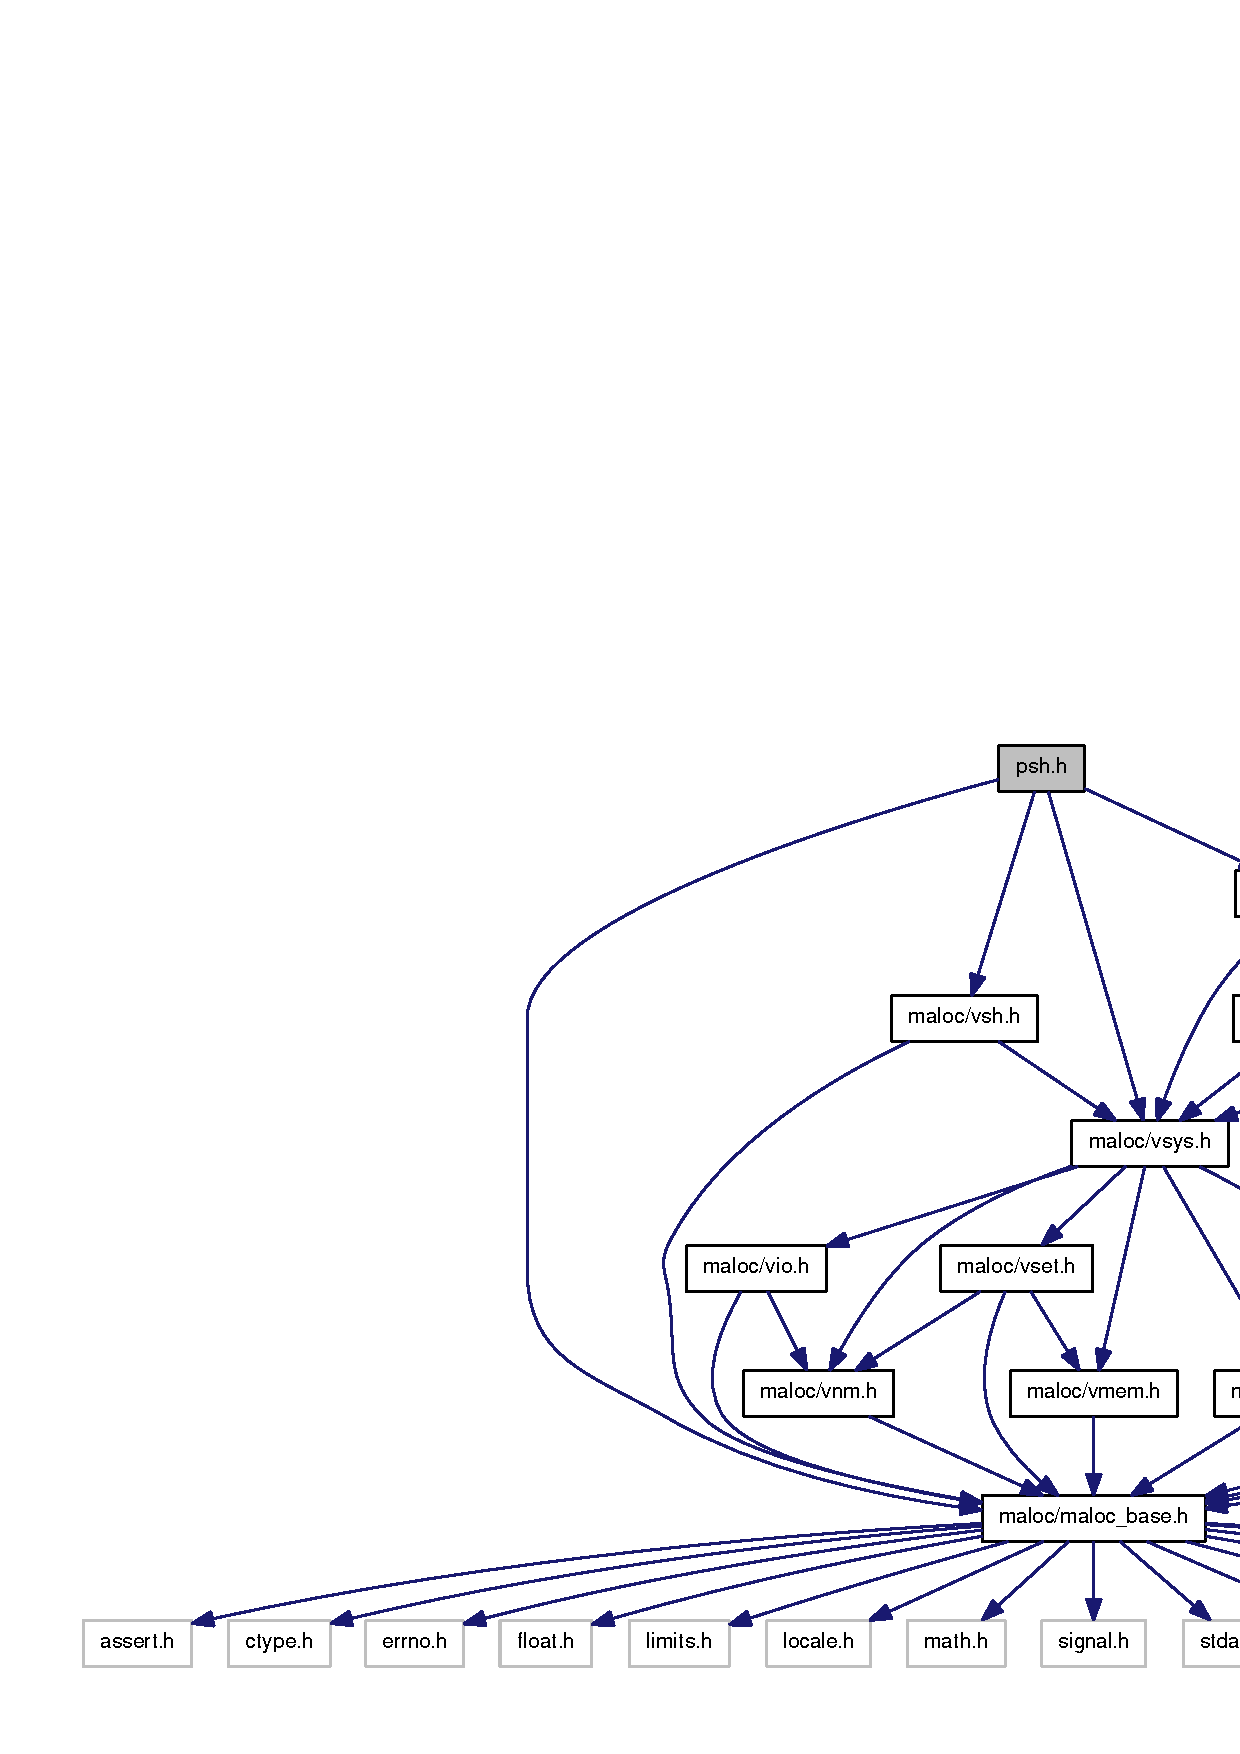
\includegraphics[width=350pt]{a00035}
\end{center}
\end{figure}
This graph shows which files directly or indirectly include this file\+:\nopagebreak
\begin{figure}[H]
\begin{center}
\leavevmode
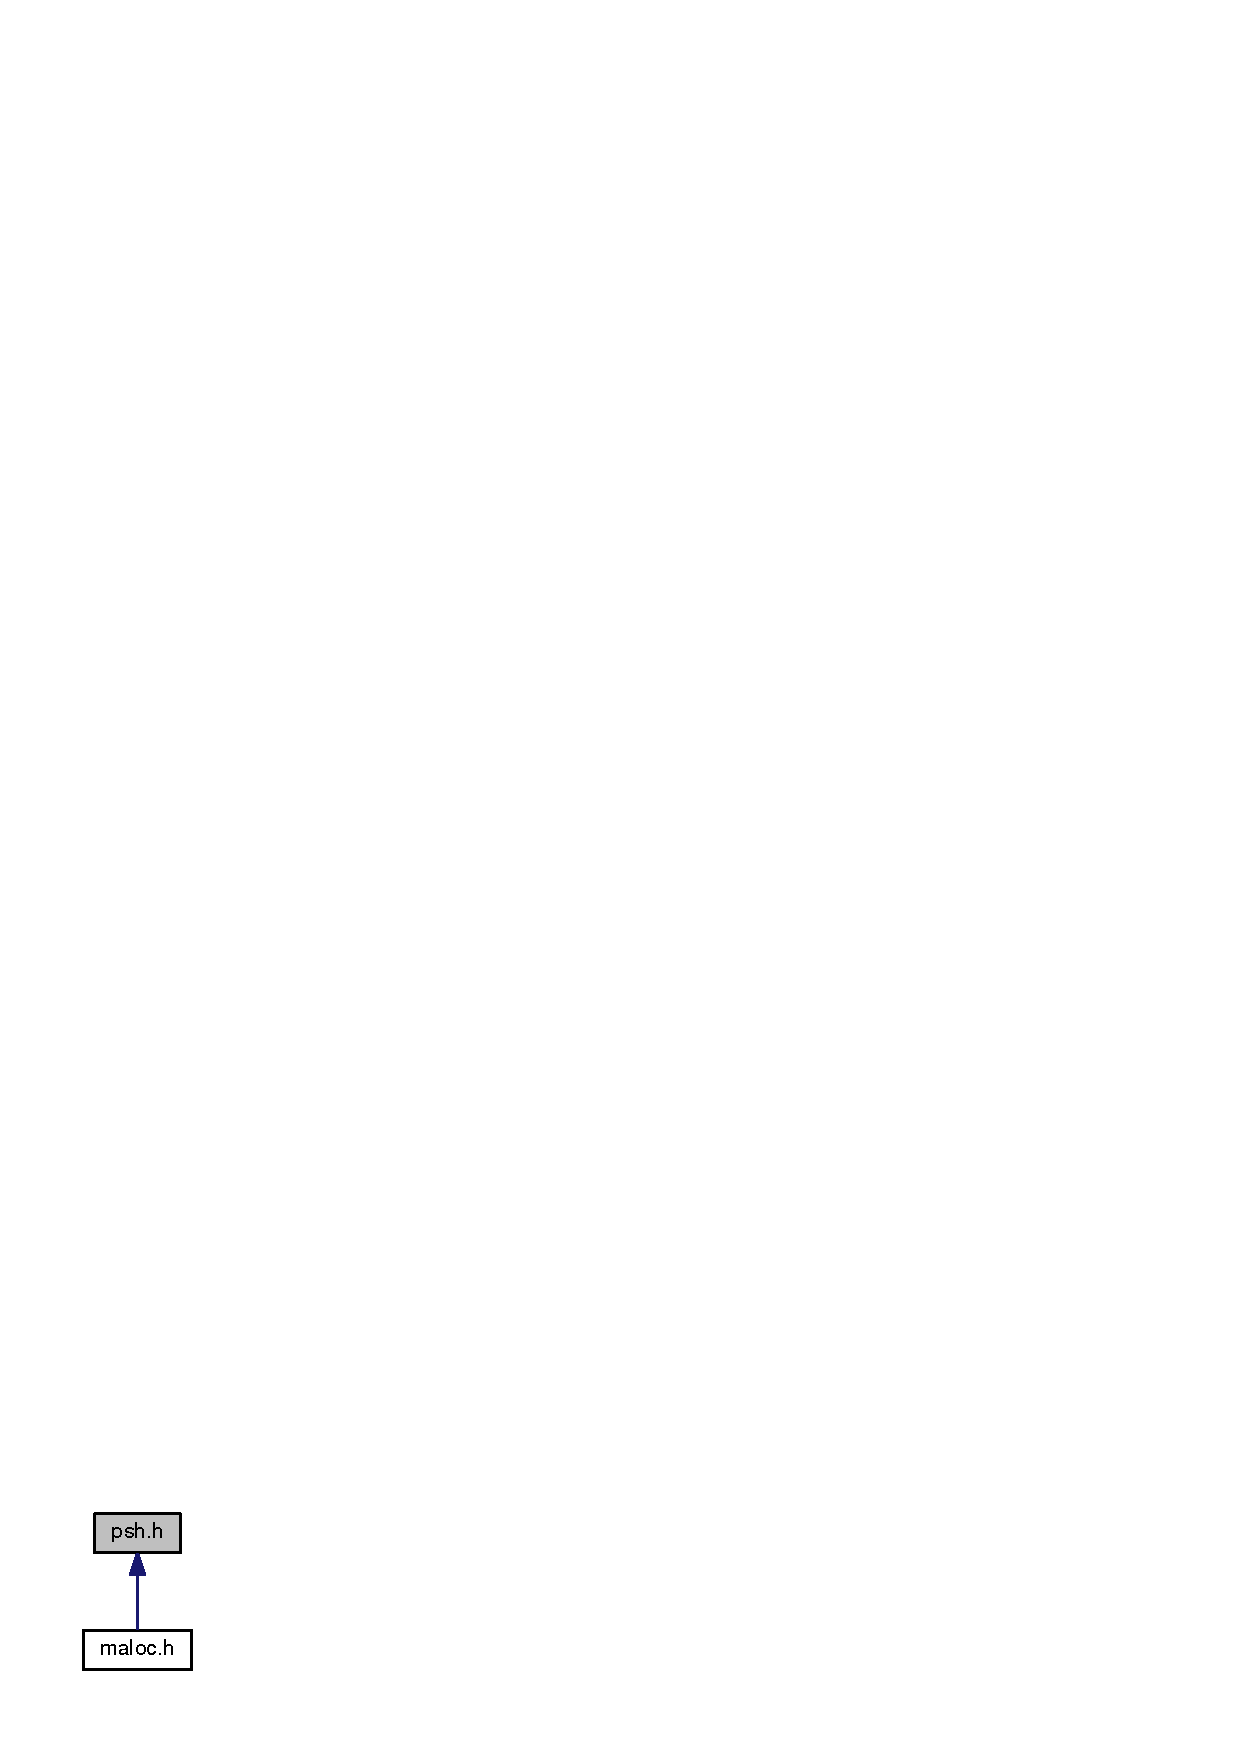
\includegraphics[width=96pt]{a00036}
\end{center}
\end{figure}
\subsection*{Functions}
\begin{DoxyCompactItemize}
\item 
int {\bf Vsh\+\_\+pshell} ({\bf Vsh} $\ast$thee, char $\ast$p\+P\+R, void $\ast$pthee, int($\ast$builtin)(void $\ast$thee, int argc, char $\ast$$\ast$argv))
\begin{DoxyCompactList}\small\item\em Drop-\/in replacement for Vsh\+\_\+shell giving parallel extensions. \end{DoxyCompactList}\end{DoxyCompactItemize}


\subsection{Detailed Description}
Header file for a simple parallel extension of A\+L\+O\+C\textquotesingle{}s V\+S\+H. 

\begin{DoxyAuthor}{Author}
Michael Holst 
\end{DoxyAuthor}
\begin{DoxyNote}{Note}
None 
\end{DoxyNote}
\begin{DoxyVersion}{Version}

\end{DoxyVersion}
\begin{DoxyParagraph}{Id}
\doxyref{psh.\+h}{p.}{a00012},v 1.\+28 2010/08/12 05\+:40\+:23 fetk Exp 
\end{DoxyParagraph}


\begin{DoxyAttention}{Attention}
\begin{DoxyVerb}*
* MALOC = < Minimal Abstraction Layer for Object-oriented C >
* Copyright (C) 1994-- Michael Holst
*
* This library is free software; you can redistribute it and/or
* modify it under the terms of the GNU Lesser General Public
* License as published by the Free Software Foundation; either
* version 2.1 of the License, or (at your option) any later version.
*
* This library is distributed in the hope that it will be useful,
* but WITHOUT ANY WARRANTY; without even the implied warranty of
* MERCHANTABILITY or FITNESS FOR A PARTICULAR PURPOSE. See the GNU
* Lesser General Public License for more details.
*
* You should have received a copy of the GNU Lesser General Public
* License along with this library; if not, write to the Free Software
* Foundation, Inc., 59 Temple Place, Suite 330, Boston, MA 02111-1307 USA
* 
*  \end{DoxyVerb}
 
\end{DoxyAttention}

\section{vcom.\-h File Reference}
\label{a00013}\index{vcom.\-h@{vcom.\-h}}


Class Vcom\-: virtual (currently just M\-P\-I) communications layer.  


{\ttfamily \#include $<$maloc/maloc\-\_\-base.\-h$>$}\\*
{\ttfamily \#include $<$maloc/vsys.\-h$>$}\\*
Include dependency graph for vcom.\-h\-:\nopagebreak
\begin{figure}[H]
\begin{center}
\leavevmode
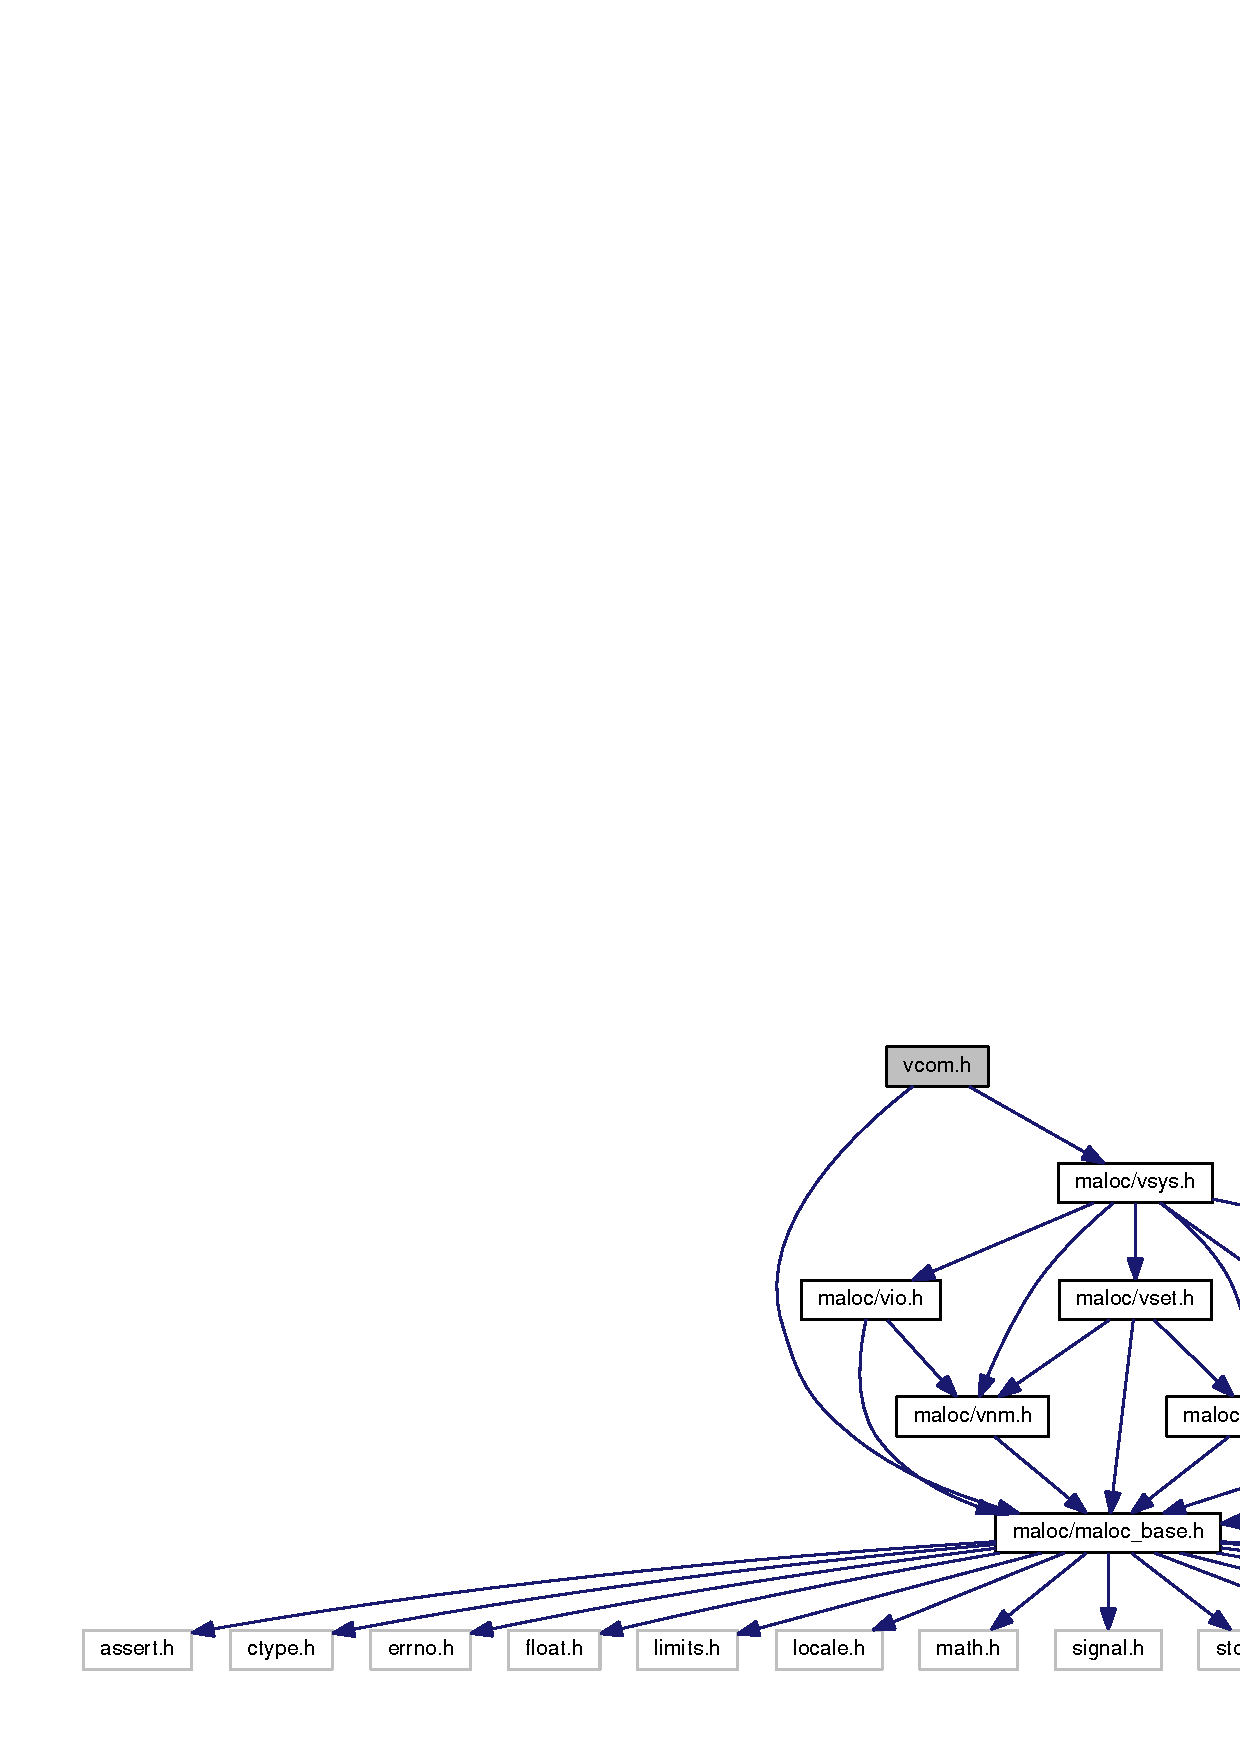
\includegraphics[width=350pt]{a00037}
\end{center}
\end{figure}
This graph shows which files directly or indirectly include this file\-:\nopagebreak
\begin{figure}[H]
\begin{center}
\leavevmode
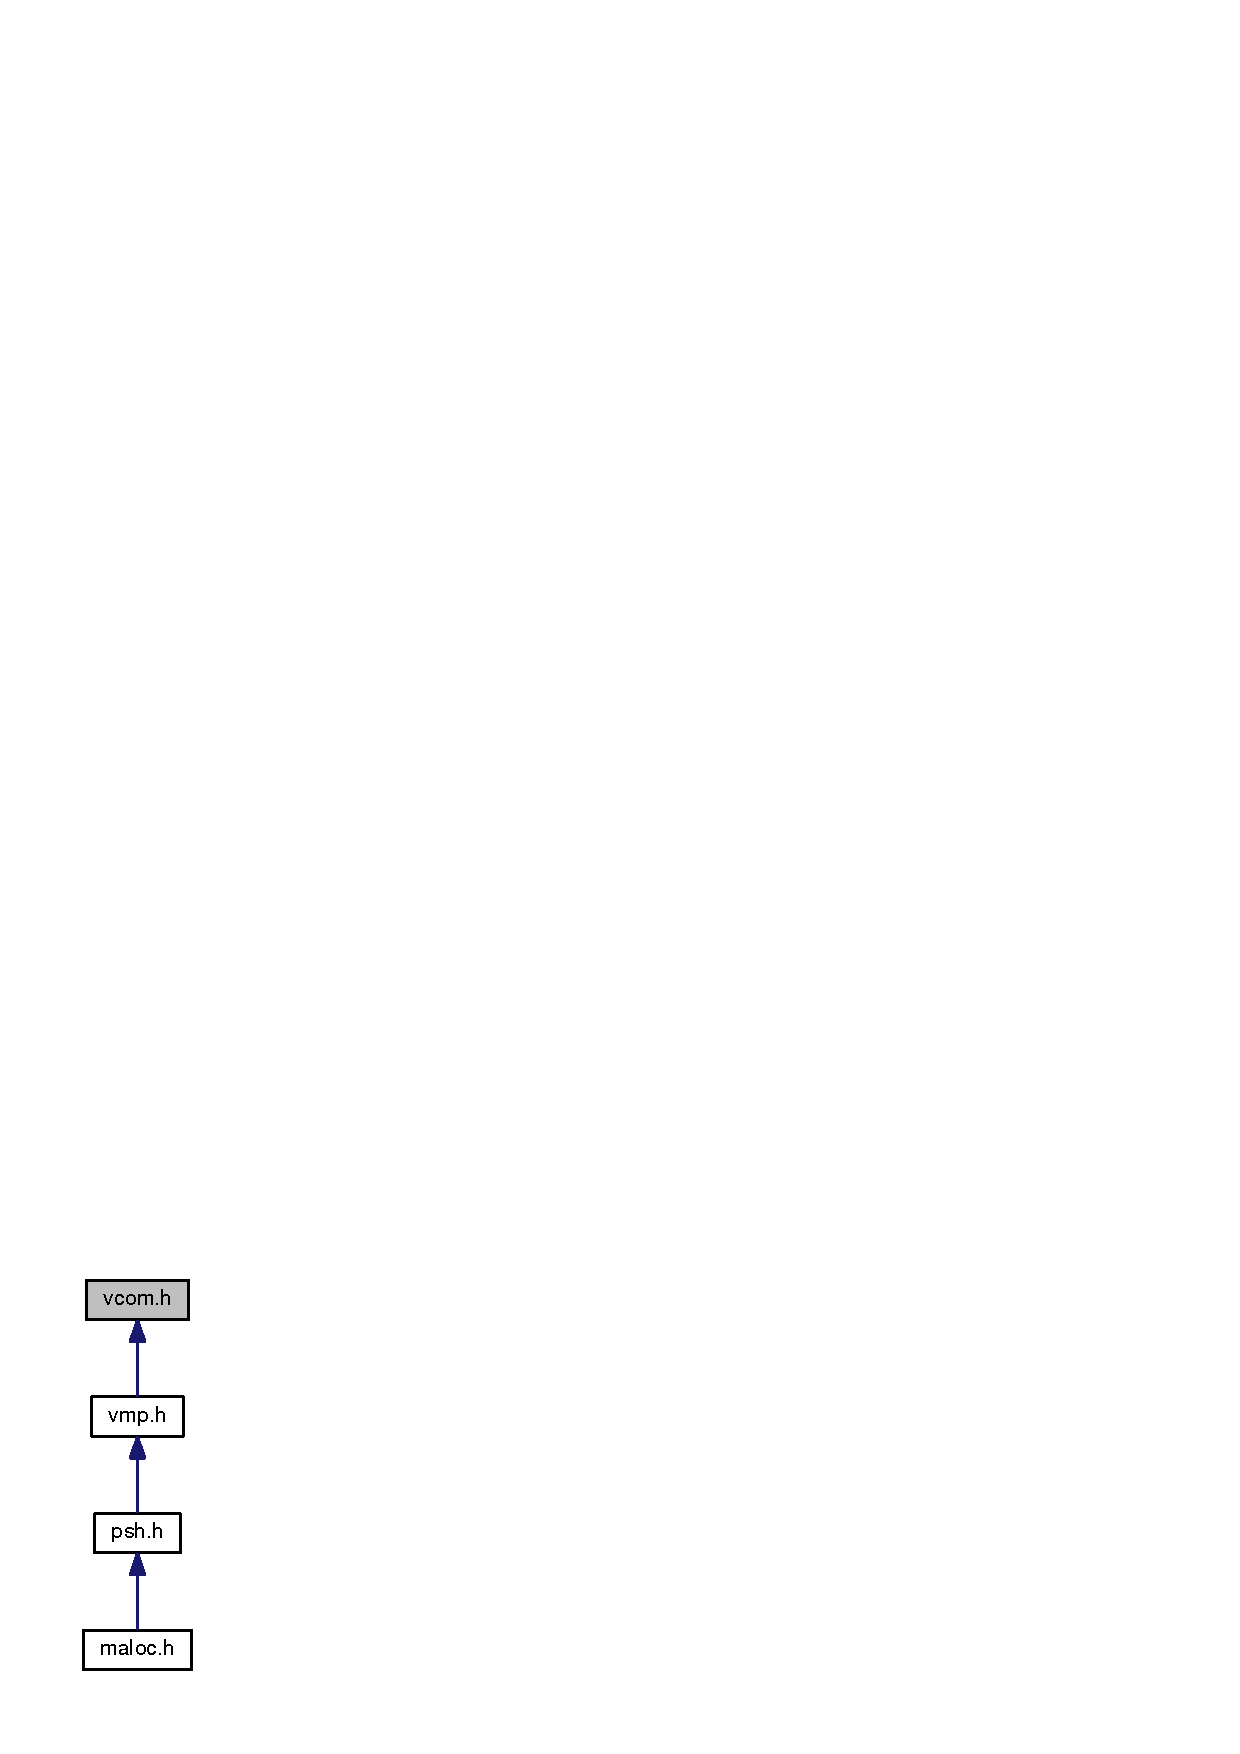
\includegraphics[width=94pt]{a00038}
\end{center}
\end{figure}
\subsection*{Classes}
\begin{DoxyCompactItemize}
\item 
struct {\bf s\-Vcom}
\begin{DoxyCompactList}\small\item\em Contains public data members for Vcom class. \end{DoxyCompactList}\end{DoxyCompactItemize}
\subsection*{Macros}
\begin{DoxyCompactItemize}
\item 
\#define {\bf V\-C\-O\-M\-\_\-\-M\-P\-I\-\_\-\-T\-A\-G}~111
\begin{DoxyCompactList}\small\item\em A base value for M\-P\-I tags. \end{DoxyCompactList}\end{DoxyCompactItemize}
\subsection*{Typedefs}
\begin{DoxyCompactItemize}
\item 
typedef struct {\bf s\-Vcom} {\bf Vcom}
\begin{DoxyCompactList}\small\item\em Declaration of the Vcom class as the Vcom structure. \end{DoxyCompactList}\end{DoxyCompactItemize}
\subsection*{Functions}
\begin{DoxyCompactItemize}
\item 
int {\bf Vcom\-\_\-init} (int $\ast$argc, char $\ast$$\ast$$\ast$argv)
\begin{DoxyCompactList}\small\item\em The Vmp initializer. \end{DoxyCompactList}\item 
int {\bf Vcom\-\_\-finalize} (void)
\begin{DoxyCompactList}\small\item\em The Vmp finalizer. \end{DoxyCompactList}\item 
{\bf Vcom} $\ast$ {\bf Vcom\-\_\-ctor} (int commtype)
\begin{DoxyCompactList}\small\item\em Construct the communications object. This routine sets up data members of class and initializes M\-P\-I. \end{DoxyCompactList}\item 
int {\bf Vcom\-\_\-ctor2} ({\bf Vcom} $\ast$thee, int commtype)
\begin{DoxyCompactList}\small\item\em Construct the communications object. This routine sets up data members of class and initializes M\-P\-I. This is broken into two parts to be callable from F\-O\-R\-T\-R\-A\-N. \end{DoxyCompactList}\item 
void {\bf Vcom\-\_\-dtor} ({\bf Vcom} $\ast$$\ast$thee)
\begin{DoxyCompactList}\small\item\em Destroy the communications object. \end{DoxyCompactList}\item 
void {\bf Vcom\-\_\-dtor2} ({\bf Vcom} $\ast$thee)
\begin{DoxyCompactList}\small\item\em Destroy the communications object. This is broken into two parts to be callable from F\-O\-R\-T\-R\-A\-N. \end{DoxyCompactList}\item 
int {\bf Vcom\-\_\-send} ({\bf Vcom} $\ast$thee, int des, void $\ast$buf, int len, int type, int block)
\begin{DoxyCompactList}\small\item\em Send a buffer. Returns 1 on success. \end{DoxyCompactList}\item 
int {\bf Vcom\-\_\-recv} ({\bf Vcom} $\ast$thee, int src, void $\ast$buf, int len, int type, int block)
\begin{DoxyCompactList}\small\item\em Receive a (character) buffer. \par
 The blocking flag is present, but not used. All receives are assumed to be blocking. A non-\/blocking receive would be {\itshape very} ugly to implement (signals or something?). \end{DoxyCompactList}\item 
int {\bf Vcom\-\_\-get\-Count} ({\bf Vcom} $\ast$thee, int src, int $\ast$length, int type)
\begin{DoxyCompactList}\small\item\em Perform a blocking probe to get the length (in number of items of specified type) of an incoming message and place it in the argument ``length". \end{DoxyCompactList}\item 
int {\bf Vcom\-\_\-reduce} ({\bf Vcom} $\ast$thee, void $\ast$sendbuf, void $\ast$recvbuf, int length, int type, int op)
\begin{DoxyCompactList}\small\item\em Perform a reduction of the data across all processors. This is equivalent (and in the case of M\-P\-I is identical to) M\-P\-I\-\_\-\-Allreduce. Basically, the specified operations are appleed to each member of the sendbuf across all processors and the results are written to recvbuf. \end{DoxyCompactList}\item 
int {\bf Vcom\-\_\-size} ({\bf Vcom} $\ast$thee)
\begin{DoxyCompactList}\small\item\em Get the number of P\-Es in communicator. \end{DoxyCompactList}\item 
int {\bf Vcom\-\_\-resize} ({\bf Vcom} $\ast$thee, int newsize)
\begin{DoxyCompactList}\small\item\em Resize (shrink) the communications group to include only newsize number of processors. \par
 Obsolete processes are given rank of -\/1 and size of 0. \end{DoxyCompactList}\item 
int {\bf Vcom\-\_\-rank} ({\bf Vcom} $\ast$thee)
\begin{DoxyCompactList}\small\item\em Get the I\-D of the local P\-E. \end{DoxyCompactList}\item 
int {\bf Vcom\-\_\-barr} ({\bf Vcom} $\ast$thee)
\begin{DoxyCompactList}\small\item\em Synchronization barrier. \end{DoxyCompactList}\end{DoxyCompactItemize}


\subsection{Detailed Description}
Class Vcom\-: virtual (currently just M\-P\-I) communications layer. \begin{DoxyAuthor}{Authors}
Nathan Baker and Michael Holst 
\end{DoxyAuthor}
\begin{DoxyNote}{Note}
None 
\end{DoxyNote}
\begin{DoxyVersion}{Version}

\end{DoxyVersion}
\begin{DoxyParagraph}{Id\-:}
\doxyref{vcom.\-h}{p.}{a00013},v 1.\-38 2010/08/12 05\-:40\-:23 fetk Exp 
\end{DoxyParagraph}


\begin{DoxyAttention}{Attention}
\begin{DoxyVerb}*
* MALOC = < Minimal Abstraction Layer for Object-oriented C >
* Copyright (C) 1994-- Michael Holst
*
* This library is free software; you can redistribute it and/or
* modify it under the terms of the GNU Lesser General Public
* License as published by the Free Software Foundation; either
* version 2.1 of the License, or (at your option) any later version.
*
* This library is distributed in the hope that it will be useful,
* but WITHOUT ANY WARRANTY; without even the implied warranty of
* MERCHANTABILITY or FITNESS FOR A PARTICULAR PURPOSE. See the GNU
* Lesser General Public License for more details.
*
* You should have received a copy of the GNU Lesser General Public
* License along with this library; if not, write to the Free Software
* Foundation, Inc., 59 Temple Place, Suite 330, Boston, MA 02111-1307 USA
* 
*  \end{DoxyVerb}
 
\end{DoxyAttention}


\subsection{Macro Definition Documentation}
\index{vcom.\-h@{vcom.\-h}!V\-C\-O\-M\-\_\-\-M\-P\-I\-\_\-\-T\-A\-G@{V\-C\-O\-M\-\_\-\-M\-P\-I\-\_\-\-T\-A\-G}}
\index{V\-C\-O\-M\-\_\-\-M\-P\-I\-\_\-\-T\-A\-G@{V\-C\-O\-M\-\_\-\-M\-P\-I\-\_\-\-T\-A\-G}!vcom.h@{vcom.\-h}}
\subsubsection[{V\-C\-O\-M\-\_\-\-M\-P\-I\-\_\-\-T\-A\-G}]{\setlength{\rightskip}{0pt plus 5cm}\#define V\-C\-O\-M\-\_\-\-M\-P\-I\-\_\-\-T\-A\-G~111}\label{a00013_a81c395f6f83ae48ed287066004e4795d}


A base value for M\-P\-I tags. 


\section{vio.h File Reference}
\label{a00014}\index{vio.h@{vio.h}}


Class Vio: virtual $<$SDIO/FILE/BUFF/UNIX/INET$>$ I/O layer.  


{\ttfamily \#include $<$maloc/maloc\_\-base.h$>$}\par
{\ttfamily \#include $<$maloc/vnm.h$>$}\par
Include dependency graph for vio.h:
\nopagebreak
\begin{figure}[H]
\begin{center}
\leavevmode
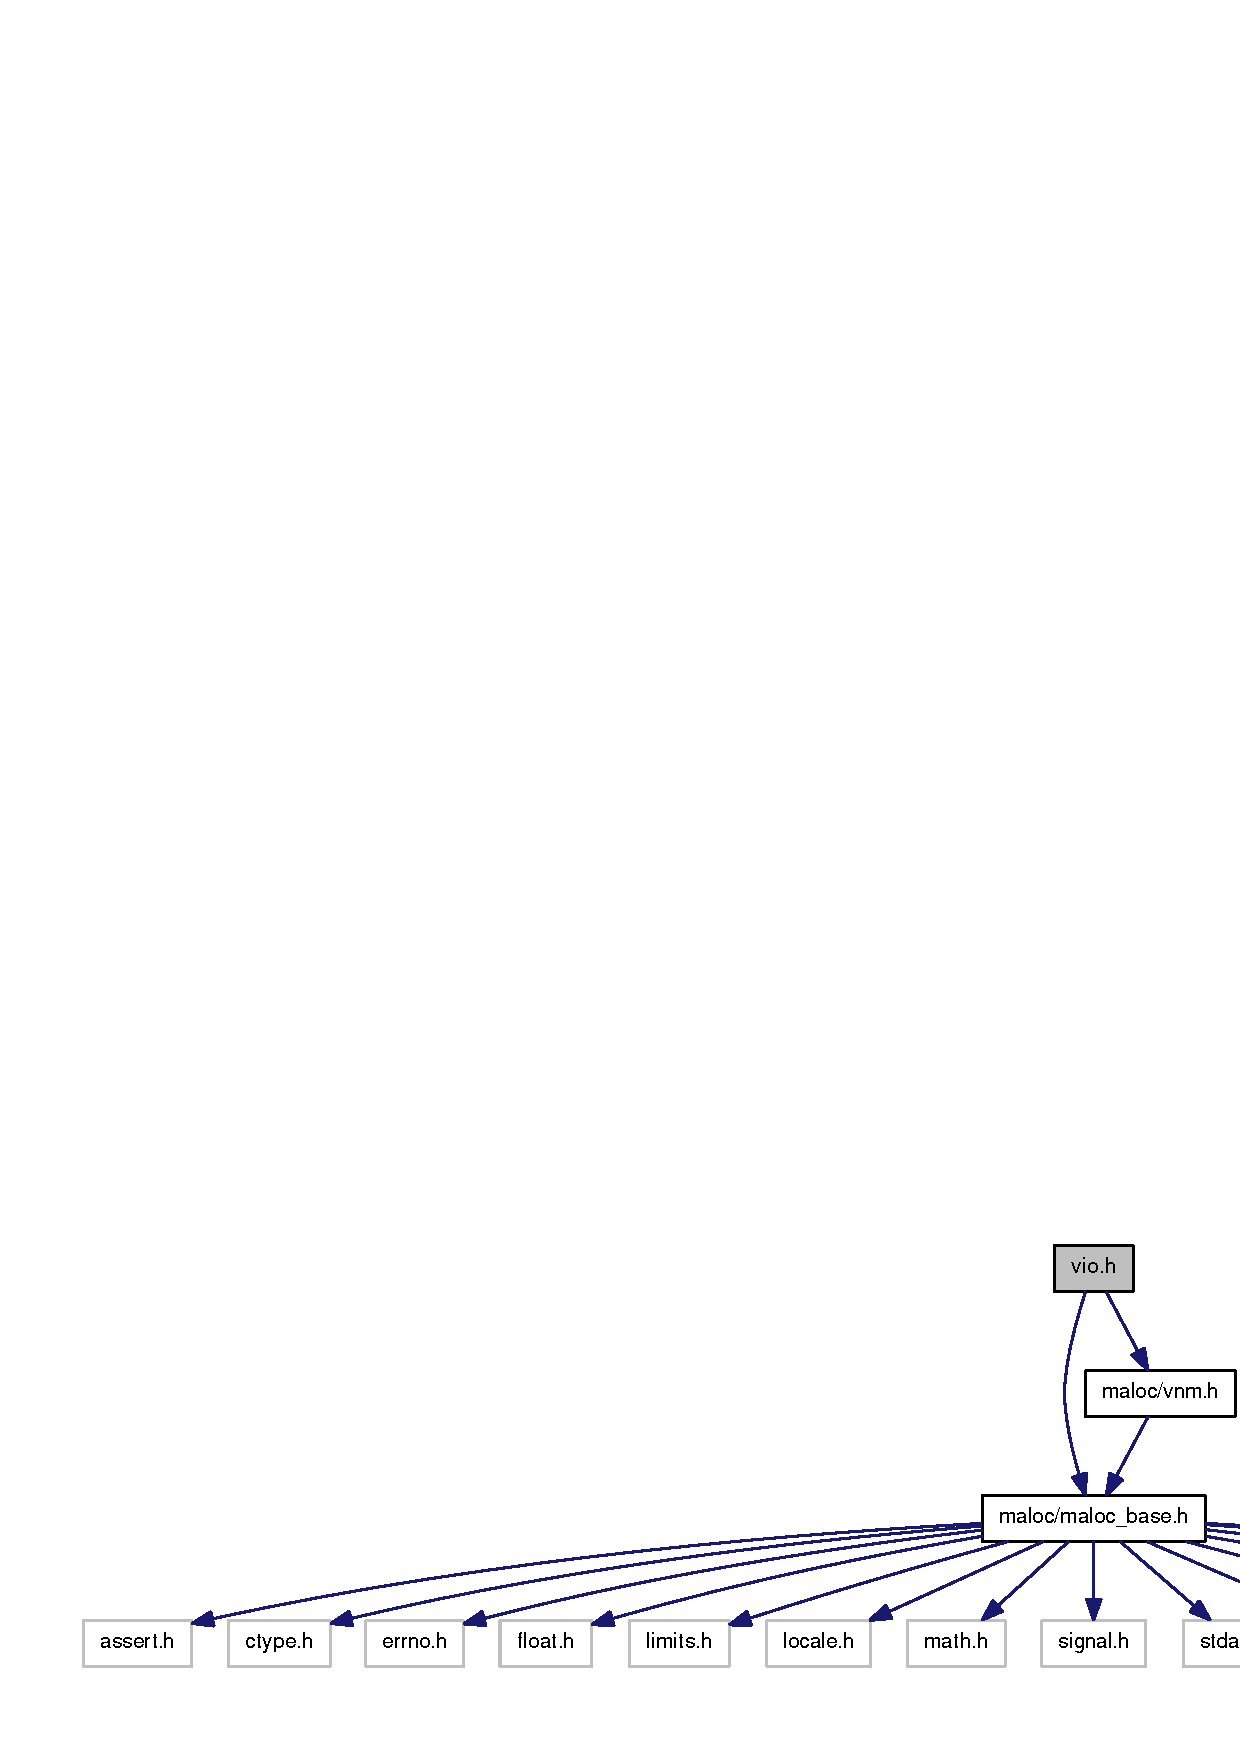
\includegraphics[width=400pt]{a00039}
\end{center}
\end{figure}
This graph shows which files directly or indirectly include this file:
\nopagebreak
\begin{figure}[H]
\begin{center}
\leavevmode
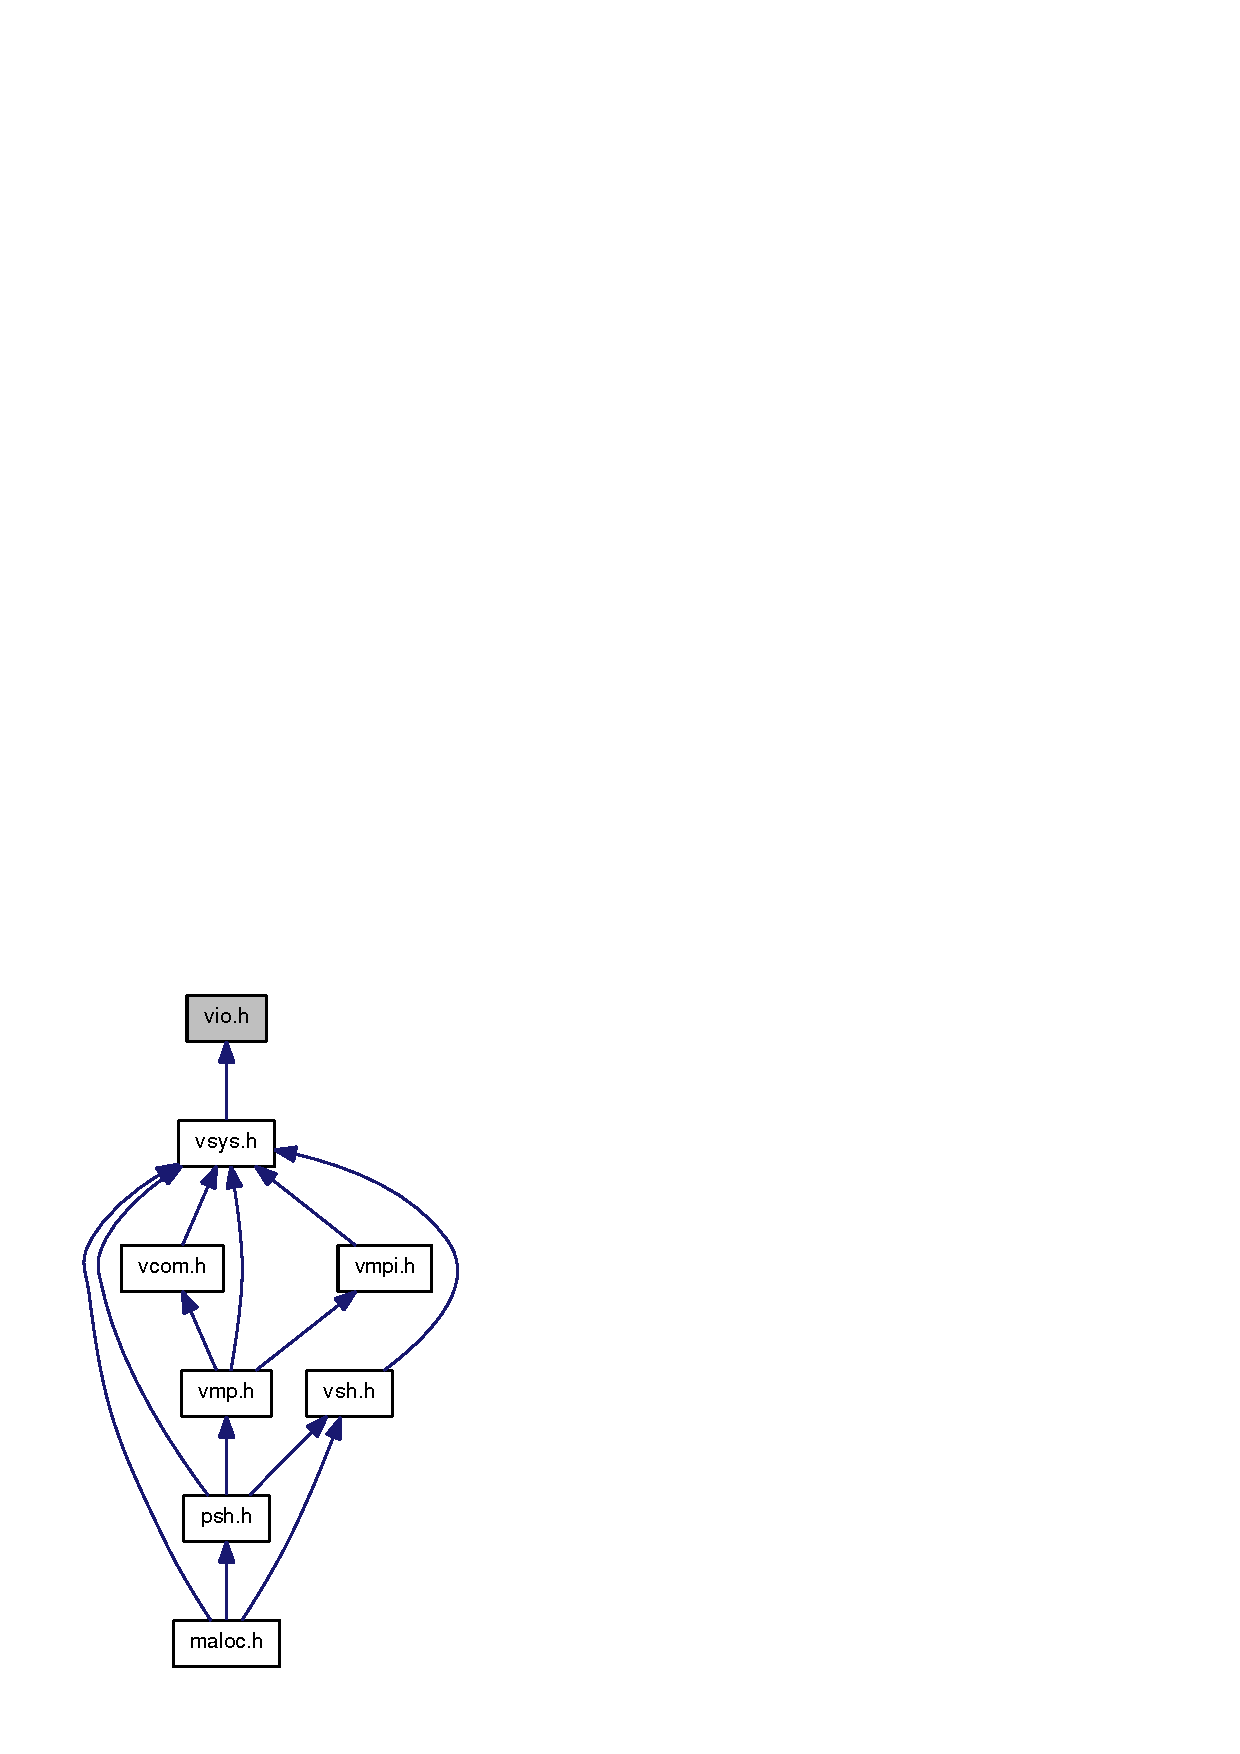
\includegraphics[width=224pt]{a00040}
\end{center}
\end{figure}
\subsection*{Classes}
\begin{DoxyCompactItemize}
\item 
struct {\bf sVio}
\begin{DoxyCompactList}\small\item\em Contains public data members for Vio class. \item\end{DoxyCompactList}\end{DoxyCompactItemize}
\subsection*{Defines}
\begin{DoxyCompactItemize}
\item 
\#define {\bf VPORTNUMBER}~14916
\begin{DoxyCompactList}\small\item\em our portbase; 5000 $<$ VPORTNUMBER $<$ 49152 \item\end{DoxyCompactList}\item 
\#define {\bf VIO\_\-MAXBUF}~10
\begin{DoxyCompactList}\small\item\em number of internal buffers (BUFF datatype) \item\end{DoxyCompactList}\end{DoxyCompactItemize}
\subsection*{Typedefs}
\begin{DoxyCompactItemize}
\item 
typedef enum {\bf VIOtype} {\bf VIOtype}
\begin{DoxyCompactList}\small\item\em Parameter for I/O type (sdio,buff,file,unix,inet). \item\end{DoxyCompactList}\item 
typedef enum {\bf VIOfrmt} {\bf VIOfrmt}
\begin{DoxyCompactList}\small\item\em Parameter for compression type (XDR,ASC). \item\end{DoxyCompactList}\item 
typedef enum {\bf VIOrwkey} {\bf VIOrwkey}
\begin{DoxyCompactList}\small\item\em Parameter for rw type (R,RW). \item\end{DoxyCompactList}\item 
typedef struct {\bf sVio} {\bf Vio}
\begin{DoxyCompactList}\small\item\em Declaration of the Vio class as the Vio structure. \item\end{DoxyCompactList}\end{DoxyCompactItemize}
\subsection*{Enumerations}
\begin{DoxyCompactItemize}
\item 
enum {\bf VIOtype} \{ \par
{\bf VIO\_\-NO\_\-TYPE}, 
{\bf VIO\_\-SDIO}, 
{\bf VIO\_\-BUFF}, 
{\bf VIO\_\-FILE}, 
\par
{\bf VIO\_\-UNIX}, 
{\bf VIO\_\-INET}
 \}
\begin{DoxyCompactList}\small\item\em Parameter for I/O type (sdio,buff,file,unix,inet). \item\end{DoxyCompactList}\item 
enum {\bf VIOfrmt} \{ {\bf VIO\_\-NO\_\-FRMT}, 
{\bf VIO\_\-XDR}, 
{\bf VIO\_\-ASC}
 \}
\begin{DoxyCompactList}\small\item\em Parameter for compression type (XDR,ASC). \item\end{DoxyCompactList}\item 
enum {\bf VIOrwkey} \{ {\bf VIO\_\-NO\_\-RW}, 
{\bf VIO\_\-R}, 
{\bf VIO\_\-W}
 \}
\begin{DoxyCompactList}\small\item\em Parameter for rw type (R,RW). \item\end{DoxyCompactList}\end{DoxyCompactItemize}
\subsection*{Functions}
\begin{DoxyCompactItemize}
\item 
void {\bf Vio\_\-start} (void)
\begin{DoxyCompactList}\small\item\em Start Vio communication layer (init internal variables/buffers). \item\end{DoxyCompactList}\item 
void {\bf Vio\_\-stop} (void)
\begin{DoxyCompactList}\small\item\em Shutdown Vio communication layer. \item\end{DoxyCompactList}\item 
{\bf Vio} $\ast$ {\bf Vio\_\-ctor} (const char $\ast$socktype, const char $\ast$datafrmt, const char $\ast$hostname, const char $\ast$filename, const char $\ast$rwkey)
\begin{DoxyCompactList}\small\item\em Construct the Vio object. \item\end{DoxyCompactList}\item 
int {\bf Vio\_\-ctor2} ({\bf Vio} $\ast$thee, const char $\ast$socktype, const char $\ast$datafrmt, const char $\ast$hostname, const char $\ast$filename, const char $\ast$rwkey)
\begin{DoxyCompactList}\small\item\em Work routine that Vio\_\-ctor calls to do most of the construction. \item\end{DoxyCompactList}\item 
void {\bf Vio\_\-dtor} ({\bf Vio} $\ast$$\ast$thee)
\begin{DoxyCompactList}\small\item\em Destruct the Vio object. \item\end{DoxyCompactList}\item 
void {\bf Vio\_\-dtor2} ({\bf Vio} $\ast$thee)
\begin{DoxyCompactList}\small\item\em Work routine that Vio\_\-dtor calls to do most of the destruction. \item\end{DoxyCompactList}\item 
void {\bf Vio\_\-setWhiteChars} ({\bf Vio} $\ast$thee, char $\ast$whiteChars)
\begin{DoxyCompactList}\small\item\em Set the white character set for I/O stream. \item\end{DoxyCompactList}\item 
void {\bf Vio\_\-setCommChars} ({\bf Vio} $\ast$thee, char $\ast$commChars)
\begin{DoxyCompactList}\small\item\em Set the comment character set for I/O stream. \item\end{DoxyCompactList}\item 
int {\bf Vio\_\-accept} ({\bf Vio} $\ast$thee, int nonblock)
\begin{DoxyCompactList}\small\item\em Accept any waiting connect attempt to our socket on our machine. \item\end{DoxyCompactList}\item 
void {\bf Vio\_\-acceptFree} ({\bf Vio} $\ast$thee)
\begin{DoxyCompactList}\small\item\em Free the socket child that was used for the last accept. \item\end{DoxyCompactList}\item 
int {\bf Vio\_\-connect} ({\bf Vio} $\ast$thee, int nonblock)
\begin{DoxyCompactList}\small\item\em Connect to some socket on a remote machine (or on our machine). \item\end{DoxyCompactList}\item 
void {\bf Vio\_\-connectFree} ({\bf Vio} $\ast$thee)
\begin{DoxyCompactList}\small\item\em Purge any output buffers (for $<$UNIX/INET$>$, else a no-\/op). \item\end{DoxyCompactList}\item 
int {\bf Vio\_\-scanf} ({\bf Vio} $\ast$thee, char $\ast$parms,...)
\begin{DoxyCompactList}\small\item\em Mimic \char`\"{}scanf\char`\"{} from an arbitrary Vio device. \item\end{DoxyCompactList}\item 
int {\bf Vio\_\-printf} ({\bf Vio} $\ast$thee, char $\ast$parms,...)
\begin{DoxyCompactList}\small\item\em Mimic \char`\"{}printf\char`\"{} from an arbitrary Vio device. \item\end{DoxyCompactList}\item 
int {\bf Vio\_\-read} ({\bf Vio} $\ast$thee, char $\ast$buf, int bufsize)
\begin{DoxyCompactList}\small\item\em Read (up to) bufsize characters into buf from input device. \item\end{DoxyCompactList}\item 
int {\bf Vio\_\-write} ({\bf Vio} $\ast$thee, char $\ast$buf, int bufsize)
\begin{DoxyCompactList}\small\item\em Write bufsize characters from buf to output device. \item\end{DoxyCompactList}\item 
void {\bf Vio\_\-bufTake} ({\bf Vio} $\ast$thee, char $\ast$buf, int bufsize)
\begin{DoxyCompactList}\small\item\em Set the pointer to the internal buffer. \item\end{DoxyCompactList}\item 
char $\ast$ {\bf Vio\_\-bufGive} ({\bf Vio} $\ast$thee)
\begin{DoxyCompactList}\small\item\em Return the pointer to the internal buffer. \item\end{DoxyCompactList}\item 
int {\bf Vio\_\-bufSize} ({\bf Vio} $\ast$thee)
\begin{DoxyCompactList}\small\item\em Return the length to the internal buffer. \item\end{DoxyCompactList}\item 
{\bf Vio} $\ast$ {\bf Vio\_\-socketOpen} (char $\ast$key, const char $\ast$iodev, const char $\ast$iofmt, const char $\ast$iohost, const char $\ast$iofile)
\begin{DoxyCompactList}\small\item\em Socket open for read or write. \item\end{DoxyCompactList}\item 
void {\bf Vio\_\-socketClose} ({\bf Vio} $\ast$$\ast$sock)
\begin{DoxyCompactList}\small\item\em Socket close from read or write. \item\end{DoxyCompactList}\end{DoxyCompactItemize}


\subsection{Detailed Description}
Class Vio: virtual $<$SDIO/FILE/BUFF/UNIX/INET$>$ I/O layer. \begin{DoxyVersion}{Version}

\end{DoxyVersion}
\begin{DoxyParagraph}{Id:}
\doxyref{vio.h}{p.}{a00014},v 1.28 2010/08/12 05:40:35 fetk Exp 
\end{DoxyParagraph}
\begin{DoxyAuthor}{Author}
Michael Holst
\end{DoxyAuthor}
\begin{DoxyAttention}{Attention}
\begin{DoxyVerb}
 *
 * MALOC = < Minimal Abstraction Layer for Object-oriented C >
 * Copyright (C) 1994-- Michael Holst
 *
 * This library is free software; you can redistribute it and/or
 * modify it under the terms of the GNU Lesser General Public
 * License as published by the Free Software Foundation; either
 * version 2.1 of the License, or (at your option) any later version.
 *
 * This library is distributed in the hope that it will be useful,
 * but WITHOUT ANY WARRANTY; without even the implied warranty of
 * MERCHANTABILITY or FITNESS FOR A PARTICULAR PURPOSE. See the GNU
 * Lesser General Public License for more details.
 *
 * You should have received a copy of the GNU Lesser General Public
 * License along with this library; if not, write to the Free Software
 * Foundation, Inc., 59 Temple Place, Suite 330, Boston, MA 02111-1307 USA
 * 
 * \end{DoxyVerb}
 
\end{DoxyAttention}


\subsection{Define Documentation}
\index{vio.h@{vio.h}!VIO\_\-MAXBUF@{VIO\_\-MAXBUF}}
\index{VIO\_\-MAXBUF@{VIO\_\-MAXBUF}!vio.h@{vio.h}}
\subsubsection[{VIO\_\-MAXBUF}]{\setlength{\rightskip}{0pt plus 5cm}\#define VIO\_\-MAXBUF~10}\label{a00014_a1e94d8ac2af32609f662f3133cb2460a}


number of internal buffers (BUFF datatype) 

\index{vio.h@{vio.h}!VPORTNUMBER@{VPORTNUMBER}}
\index{VPORTNUMBER@{VPORTNUMBER}!vio.h@{vio.h}}
\subsubsection[{VPORTNUMBER}]{\setlength{\rightskip}{0pt plus 5cm}\#define VPORTNUMBER~14916}\label{a00014_a4a7675dfbe5a786fba616dba632bb44a}


our portbase; 5000 $<$ VPORTNUMBER $<$ 49152 


\section{vmem.\-h File Reference}
\label{a00015}\index{vmem.\-h@{vmem.\-h}}


Class Vmem\-: A safer, object-\/oriented, malloc/free object.  


{\ttfamily \#include $<$maloc/maloc\-\_\-base.\-h$>$}\\*
Include dependency graph for vmem.\-h\-:\nopagebreak
\begin{figure}[H]
\begin{center}
\leavevmode
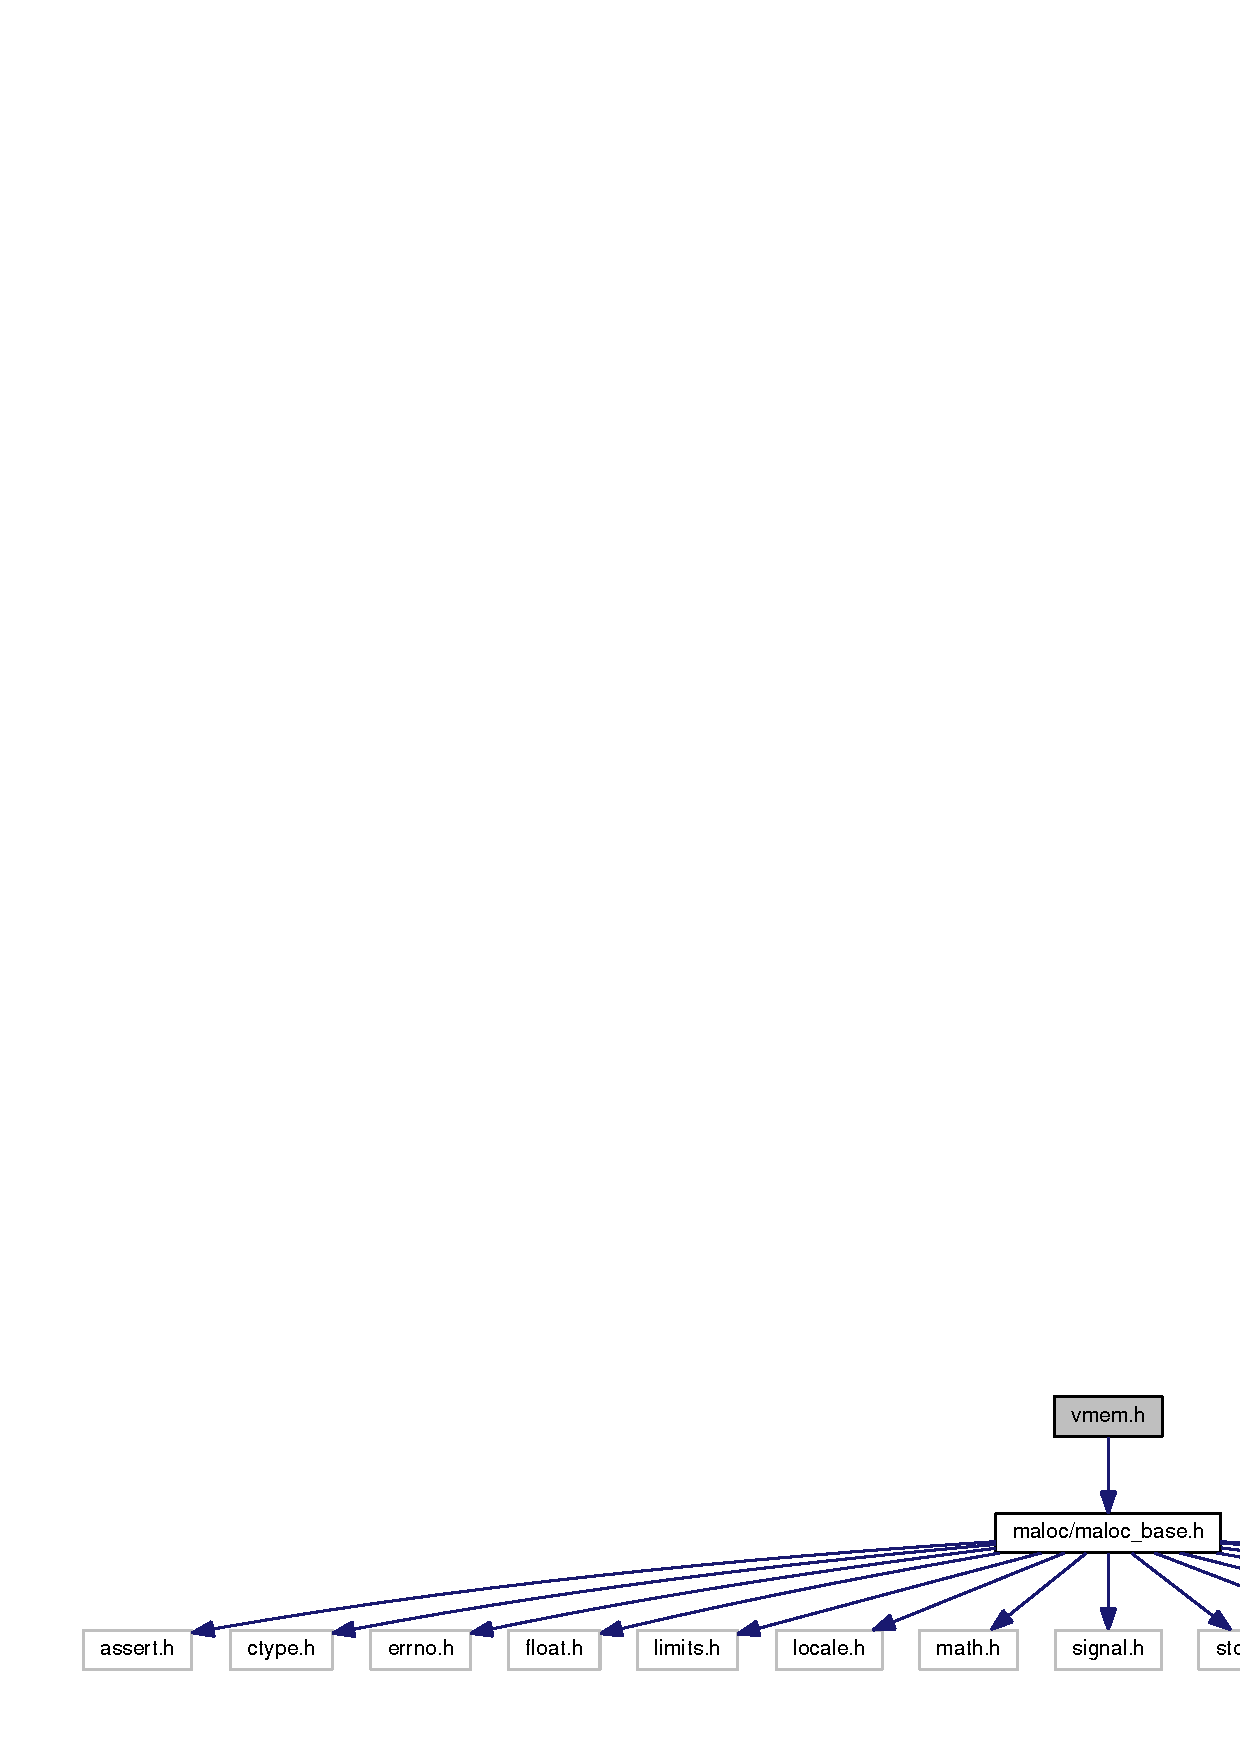
\includegraphics[width=350pt]{a00041}
\end{center}
\end{figure}
This graph shows which files directly or indirectly include this file\-:\nopagebreak
\begin{figure}[H]
\begin{center}
\leavevmode
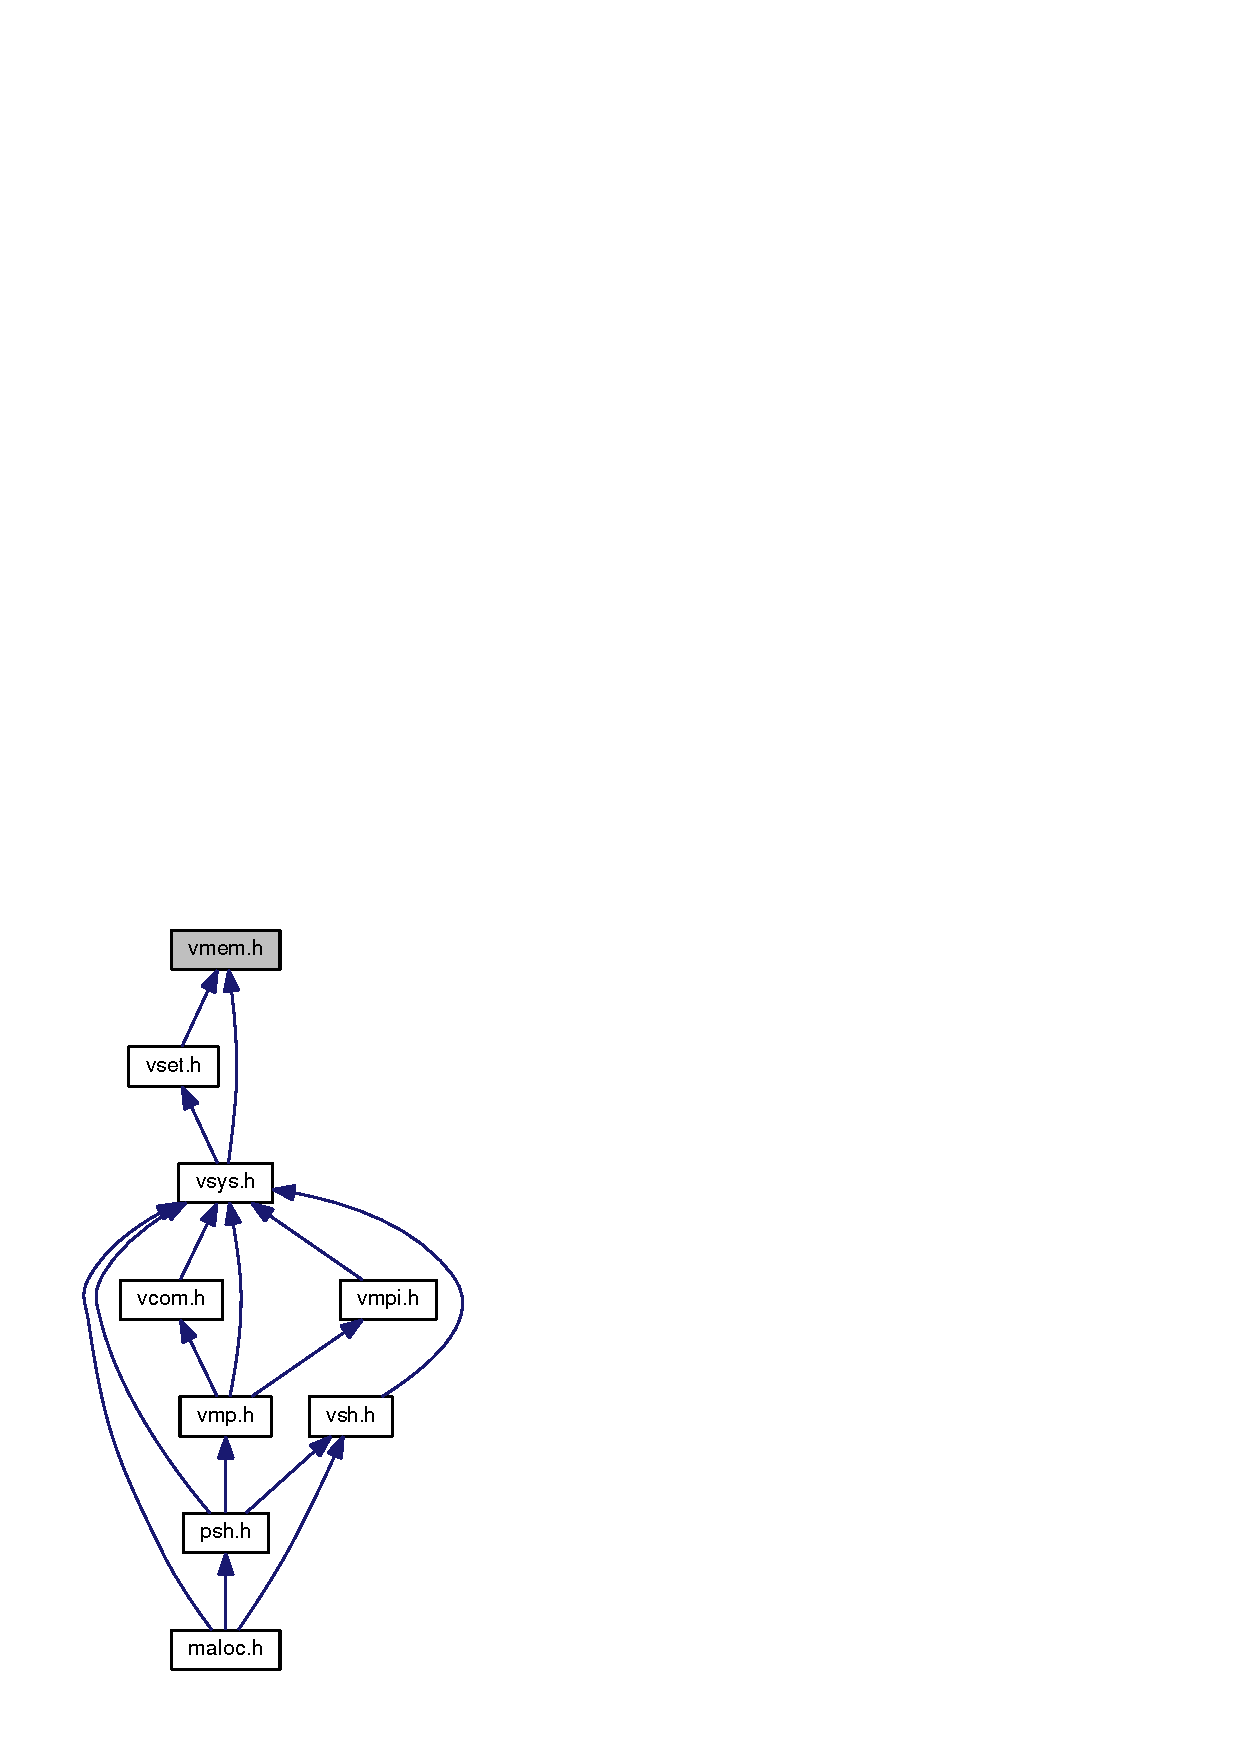
\includegraphics[width=222pt]{a00042}
\end{center}
\end{figure}
\subsection*{Classes}
\begin{DoxyCompactItemize}
\item 
struct {\bf s\-Vmem}
\begin{DoxyCompactList}\small\item\em Contains public data members for Vmem class. \end{DoxyCompactList}\end{DoxyCompactItemize}
\subsection*{Typedefs}
\begin{DoxyCompactItemize}
\item 
typedef struct {\bf s\-Vmem} {\bf Vmem}
\begin{DoxyCompactList}\small\item\em Declaration of the Vmem class as the Vmem structure. \end{DoxyCompactList}\end{DoxyCompactItemize}
\subsection*{Functions}
\begin{DoxyCompactItemize}
\item 
size\-\_\-t {\bf Vmem\-\_\-bytes\-Total} (void)
\begin{DoxyCompactList}\small\item\em Return total of all active Vmem malloc areas (current footprint) \end{DoxyCompactList}\item 
size\-\_\-t {\bf Vmem\-\_\-malloc\-Bytes\-Total} (void)
\begin{DoxyCompactList}\small\item\em Return total of all Vmem malloc allocations. \end{DoxyCompactList}\item 
size\-\_\-t {\bf Vmem\-\_\-free\-Bytes\-Total} (void)
\begin{DoxyCompactList}\small\item\em Return total of all Vmem free calls. \end{DoxyCompactList}\item 
size\-\_\-t {\bf Vmem\-\_\-high\-Water\-Total} (void)
\begin{DoxyCompactList}\small\item\em Return the high-\/water byte mark (largest footprint) \end{DoxyCompactList}\item 
size\-\_\-t {\bf Vmem\-\_\-malloc\-Areas\-Total} (void)
\begin{DoxyCompactList}\small\item\em Return total of all active Vmem malloc areas by groups. \end{DoxyCompactList}\item 
void {\bf Vmem\-\_\-print\-Total} (void)
\begin{DoxyCompactList}\small\item\em Print current memory statistics for all Vmem malloc/free areas. \end{DoxyCompactList}\item 
{\bf Vmem} $\ast$ {\bf Vmem\-\_\-ctor} (char $\ast$name)
\begin{DoxyCompactList}\small\item\em Construct the dynamic memory allocation logging object. \end{DoxyCompactList}\item 
void {\bf Vmem\-\_\-dtor} ({\bf Vmem} $\ast$$\ast$thee)
\begin{DoxyCompactList}\small\item\em Destruct the dynamic memory allocation logging object. \end{DoxyCompactList}\item 
void $\ast$ {\bf Vmem\-\_\-malloc} ({\bf Vmem} $\ast$thee, size\-\_\-t num, size\-\_\-t size)
\begin{DoxyCompactList}\small\item\em A safe logged version of malloc. \end{DoxyCompactList}\item 
void {\bf Vmem\-\_\-free} ({\bf Vmem} $\ast$thee, size\-\_\-t num, size\-\_\-t size, void $\ast$$\ast$ram)
\begin{DoxyCompactList}\small\item\em A safe logged version of free. \end{DoxyCompactList}\item 
void $\ast$ {\bf Vmem\-\_\-realloc} ({\bf Vmem} $\ast$thee, size\-\_\-t num, size\-\_\-t size, void $\ast$$\ast$ram, size\-\_\-t new\-Num)
\begin{DoxyCompactList}\small\item\em A safe logged version of realloc (usually a bad idea to use this) \end{DoxyCompactList}\item 
size\-\_\-t {\bf Vmem\-\_\-bytes} ({\bf Vmem} $\ast$thee)
\begin{DoxyCompactList}\small\item\em Return total of all A\-C\-T\-I\-V\-E malloc areas used by Vmem object. \end{DoxyCompactList}\item 
size\-\_\-t {\bf Vmem\-\_\-malloc\-Bytes} ({\bf Vmem} $\ast$thee)
\begin{DoxyCompactList}\small\item\em Return total of all mallocs performed by Vmem object. \end{DoxyCompactList}\item 
size\-\_\-t {\bf Vmem\-\_\-free\-Bytes} ({\bf Vmem} $\ast$thee)
\begin{DoxyCompactList}\small\item\em Return total of all frees performed by Vmem object. \end{DoxyCompactList}\item 
size\-\_\-t {\bf Vmem\-\_\-high\-Water} ({\bf Vmem} $\ast$thee)
\begin{DoxyCompactList}\small\item\em Return high-\/water malloc bytemark hit by Vmem object. \end{DoxyCompactList}\item 
size\-\_\-t {\bf Vmem\-\_\-malloc\-Areas} ({\bf Vmem} $\ast$thee)
\begin{DoxyCompactList}\small\item\em Return total number of individual active malloc areas. \end{DoxyCompactList}\item 
void {\bf Vmem\-\_\-print} ({\bf Vmem} $\ast$thee)
\begin{DoxyCompactList}\small\item\em Print current memory stats associated with this Vmem object. \end{DoxyCompactList}\end{DoxyCompactItemize}


\subsection{Detailed Description}
Class Vmem\-: A safer, object-\/oriented, malloc/free object. \begin{DoxyAuthor}{Author}
Michael Holst 
\end{DoxyAuthor}
\begin{DoxyNote}{Note}
None 
\end{DoxyNote}
\begin{DoxyVersion}{Version}

\end{DoxyVersion}
\begin{DoxyParagraph}{Id\-:}
\doxyref{vmem.\-h}{p.}{a00015},v 1.\-21 2010/08/12 05\-:40\-:36 fetk Exp 
\end{DoxyParagraph}


\begin{DoxyAttention}{Attention}
\begin{DoxyVerb}*
* MALOC = < Minimal Abstraction Layer for Object-oriented C >
* Copyright (C) 1994-- Michael Holst
*
* This library is free software; you can redistribute it and/or
* modify it under the terms of the GNU Lesser General Public
* License as published by the Free Software Foundation; either
* version 2.1 of the License, or (at your option) any later version.
*
* This library is distributed in the hope that it will be useful,
* but WITHOUT ANY WARRANTY; without even the implied warranty of
* MERCHANTABILITY or FITNESS FOR A PARTICULAR PURPOSE. See the GNU
* Lesser General Public License for more details.
*
* You should have received a copy of the GNU Lesser General Public
* License along with this library; if not, write to the Free Software
* Foundation, Inc., 59 Temple Place, Suite 330, Boston, MA 02111-1307 USA
* 
* \end{DoxyVerb}
 
\end{DoxyAttention}

\section{vmp.h File Reference}
\label{a00016}\index{vmp.h@{vmp.h}}


Class Vmp: a Virtual MPI communication layer object.  


{\ttfamily \#include $<$maloc/maloc\_\-base.h$>$}\par
{\ttfamily \#include $<$maloc/vsys.h$>$}\par
{\ttfamily \#include $<$maloc/vmpi.h$>$}\par
{\ttfamily \#include $<$maloc/vcom.h$>$}\par
Include dependency graph for vmp.h:
\nopagebreak
\begin{figure}[H]
\begin{center}
\leavevmode
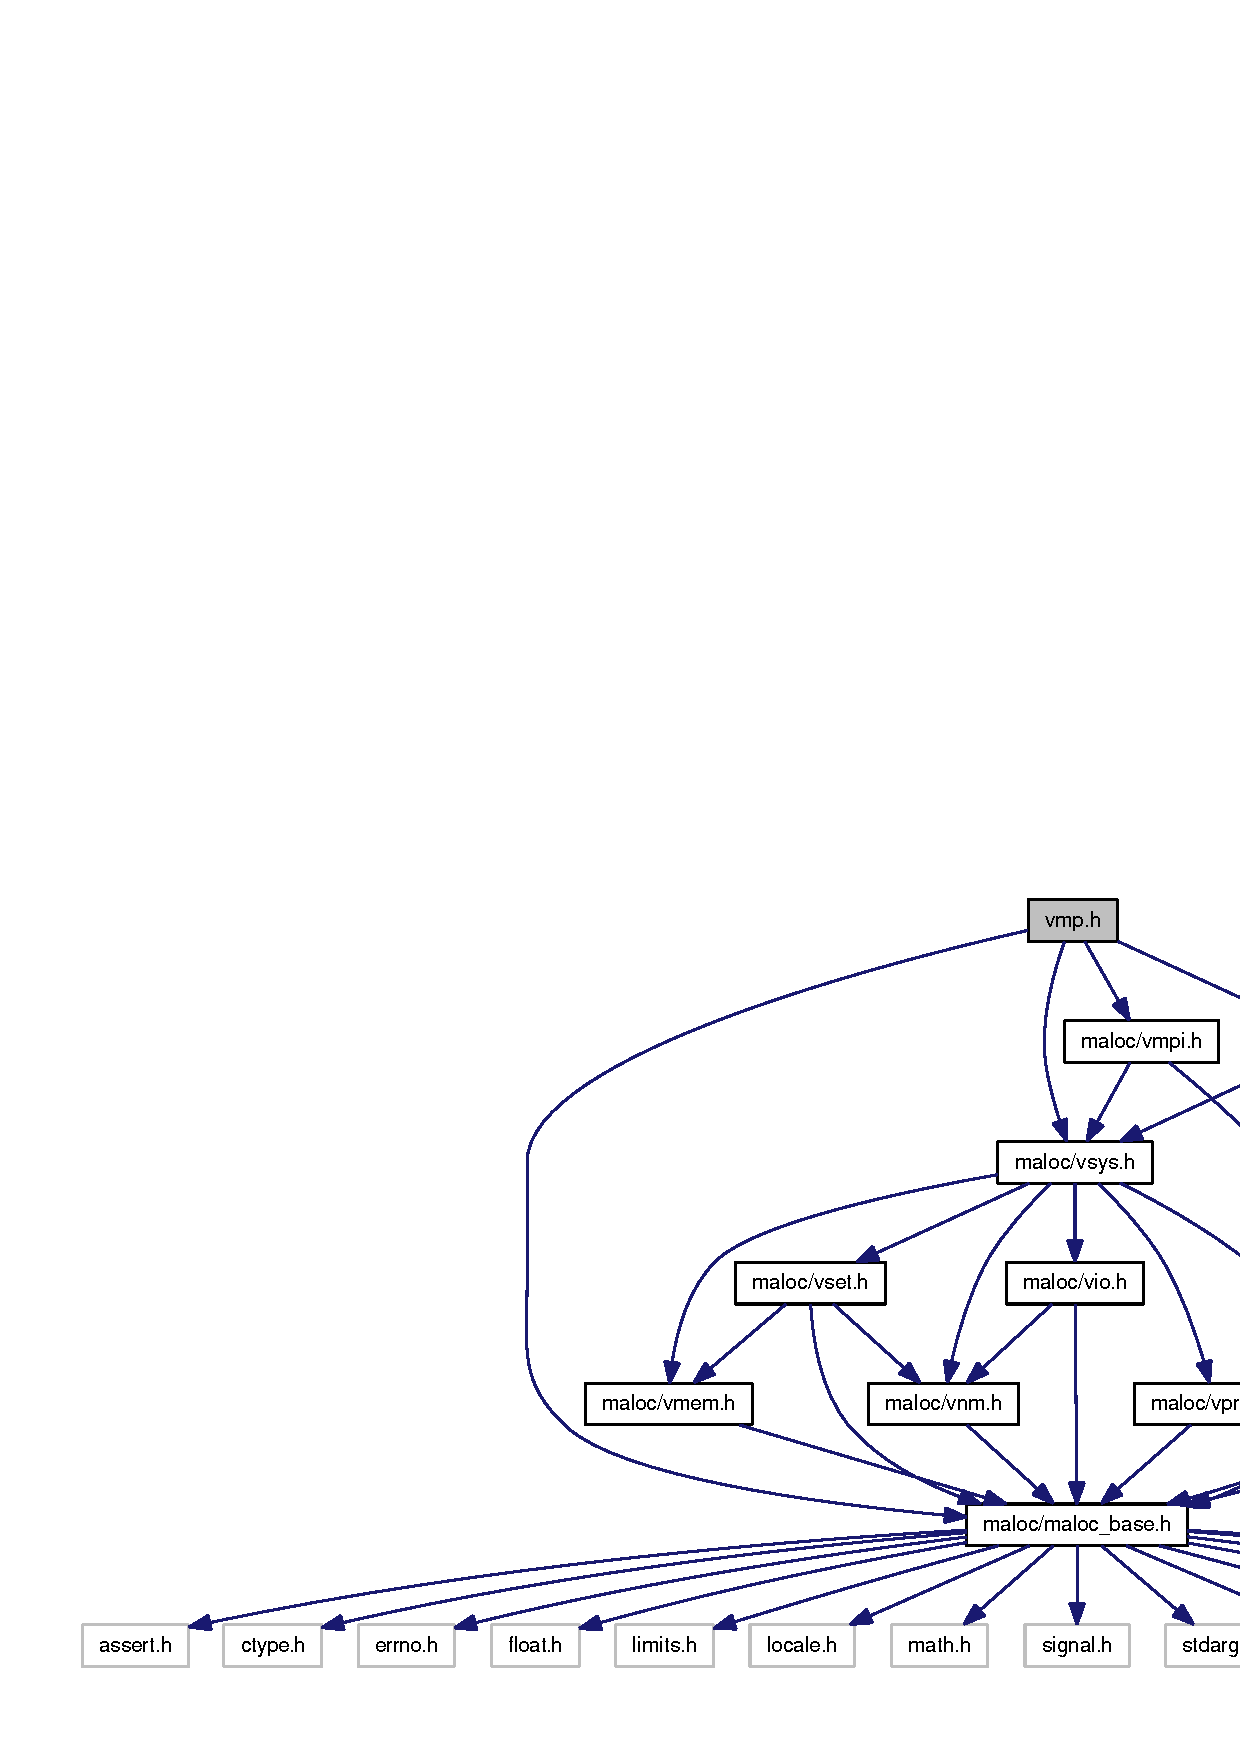
\includegraphics[width=400pt]{a00043}
\end{center}
\end{figure}
This graph shows which files directly or indirectly include this file:
\nopagebreak
\begin{figure}[H]
\begin{center}
\leavevmode
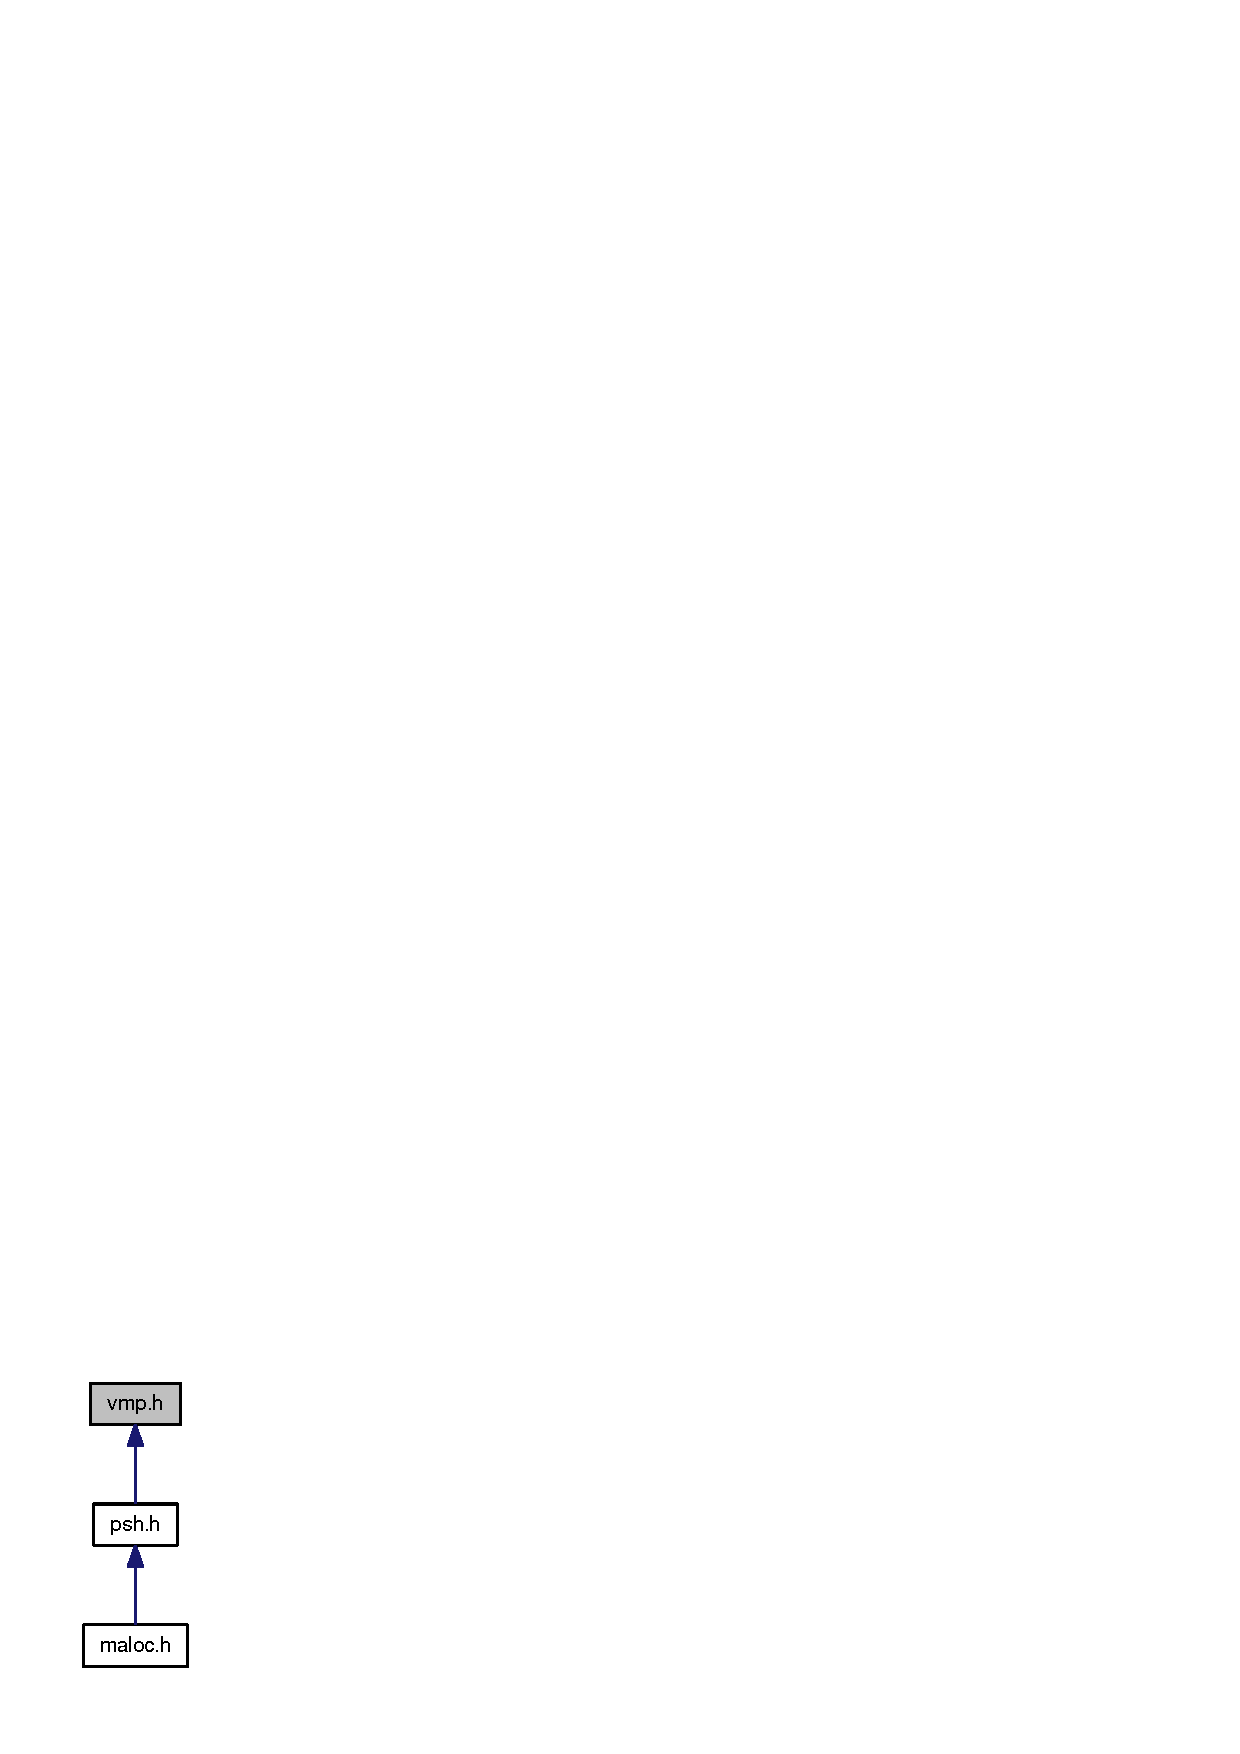
\includegraphics[width=94pt]{a00044}
\end{center}
\end{figure}
\subsection*{Classes}
\begin{DoxyCompactItemize}
\item 
struct {\bf sVmp}
\begin{DoxyCompactList}\small\item\em Contains public data members for Vmp class. \item\end{DoxyCompactList}\end{DoxyCompactItemize}
\subsection*{Typedefs}
\begin{DoxyCompactItemize}
\item 
typedef struct {\bf sVmp} {\bf Vmp}
\begin{DoxyCompactList}\small\item\em Declaration of the Vmp class as teh Vmp structure. \item\end{DoxyCompactList}\end{DoxyCompactItemize}
\subsection*{Functions}
\begin{DoxyCompactItemize}
\item 
int {\bf Vmp\_\-init} (int $\ast$argc, char $\ast$$\ast$$\ast$argv)
\begin{DoxyCompactList}\small\item\em The Vmp initializer. \item\end{DoxyCompactList}\item 
int {\bf Vmp\_\-finalize} (void)
\begin{DoxyCompactList}\small\item\em The Vmp finalizer. \item\end{DoxyCompactList}\item 
{\bf Vmp} $\ast$ {\bf Vmp\_\-ctor} (void)
\begin{DoxyCompactList}\small\item\em The Vmp constructor. \item\end{DoxyCompactList}\item 
void {\bf Vmp\_\-dtor} ({\bf Vmp} $\ast$$\ast$thee)
\begin{DoxyCompactList}\small\item\em The Vmp destructor. \item\end{DoxyCompactList}\item 
int {\bf Vmp\_\-rank} ({\bf Vmp} $\ast$thee)
\begin{DoxyCompactList}\small\item\em Return my processor ID. \item\end{DoxyCompactList}\item 
int {\bf Vmp\_\-size} ({\bf Vmp} $\ast$thee)
\begin{DoxyCompactList}\small\item\em Return the number of processors involved. \item\end{DoxyCompactList}\item 
int {\bf Vmp\_\-barr} ({\bf Vmp} $\ast$thee)
\begin{DoxyCompactList}\small\item\em An MPI barrier. \item\end{DoxyCompactList}\item 
int {\bf Vmp\_\-send} ({\bf Vmp} $\ast$thee, int des, char $\ast$buf, int bufsize)
\begin{DoxyCompactList}\small\item\em An MPI blocking send. \item\end{DoxyCompactList}\item 
int {\bf Vmp\_\-recv} ({\bf Vmp} $\ast$thee, int src, char $\ast$buf, int bufsize)
\begin{DoxyCompactList}\small\item\em An MPI blocking receive. \item\end{DoxyCompactList}\end{DoxyCompactItemize}


\subsection{Detailed Description}
Class Vmp: a Virtual MPI communication layer object. \begin{DoxyAuthor}{Author}
Michael Holst 
\end{DoxyAuthor}
\begin{DoxyNote}{Note}
None 
\end{DoxyNote}
\begin{DoxyVersion}{Version}

\end{DoxyVersion}
\begin{DoxyParagraph}{Id:}
\doxyref{vmp.h}{p.}{a00016},v 1.22 2010/08/12 05:40:23 fetk Exp 
\end{DoxyParagraph}


\begin{DoxyAttention}{Attention}
\begin{DoxyVerb}
 *
 * MALOC = < Minimal Abstraction Layer for Object-oriented C >
 * Copyright (C) 1994-- Michael Holst
 *
 * This library is free software; you can redistribute it and/or
 * modify it under the terms of the GNU Lesser General Public
 * License as published by the Free Software Foundation; either
 * version 2.1 of the License, or (at your option) any later version.
 *
 * This library is distributed in the hope that it will be useful,
 * but WITHOUT ANY WARRANTY; without even the implied warranty of
 * MERCHANTABILITY or FITNESS FOR A PARTICULAR PURPOSE. See the GNU
 * Lesser General Public License for more details.
 *
 * You should have received a copy of the GNU Lesser General Public
 * License along with this library; if not, write to the Free Software
 * Foundation, Inc., 59 Temple Place, Suite 330, Boston, MA 02111-1307 USA
 * 
 *  \end{DoxyVerb}
 
\end{DoxyAttention}

\section{vmpi.\+h File Reference}
\label{a00017}\index{vmpi.\+h@{vmpi.\+h}}


Class Vmpi\+: a Virtual M\+P\+I communication layer object.  


{\ttfamily \#include $<$maloc/maloc\+\_\+base.\+h$>$}\\*
{\ttfamily \#include $<$maloc/vsys.\+h$>$}\\*
Include dependency graph for vmpi.\+h\+:\nopagebreak
\begin{figure}[H]
\begin{center}
\leavevmode
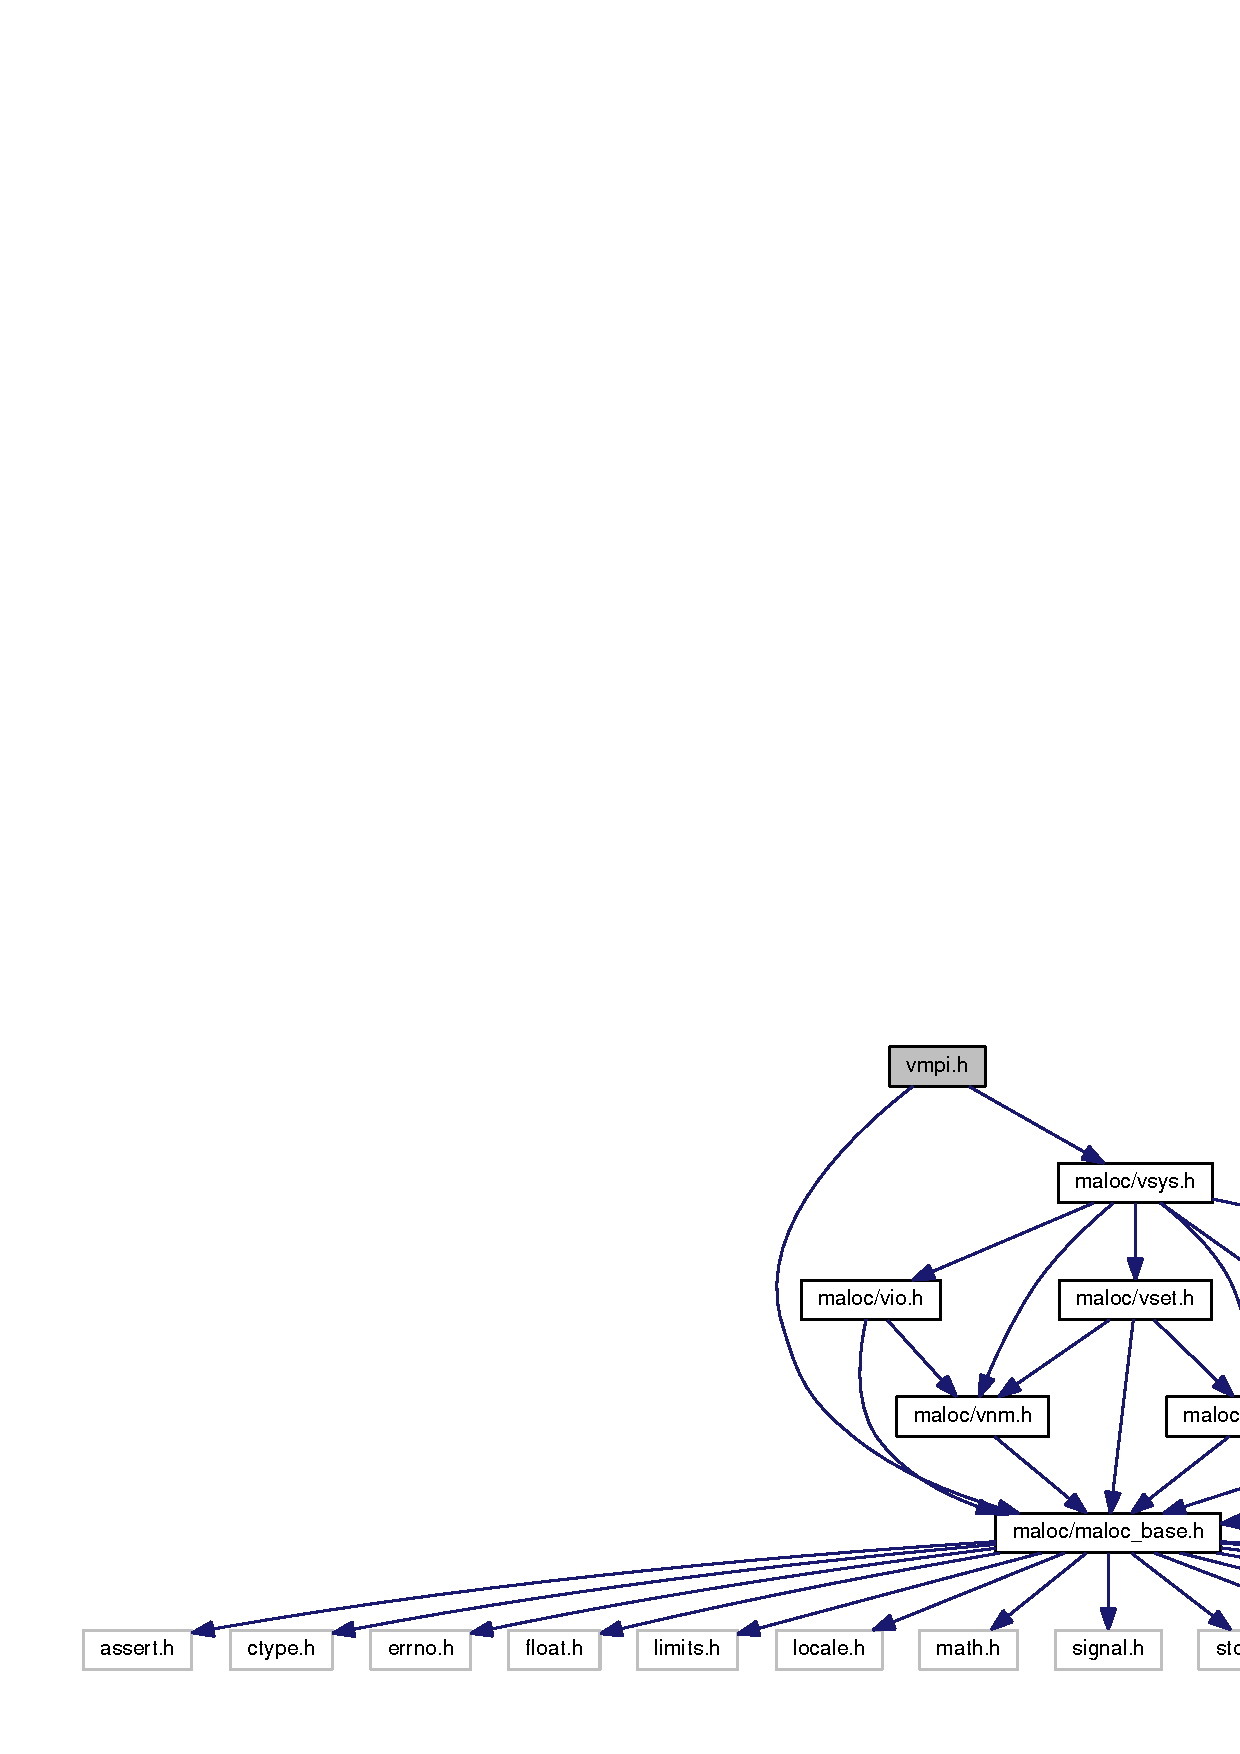
\includegraphics[width=350pt]{a00045}
\end{center}
\end{figure}
This graph shows which files directly or indirectly include this file\+:\nopagebreak
\begin{figure}[H]
\begin{center}
\leavevmode
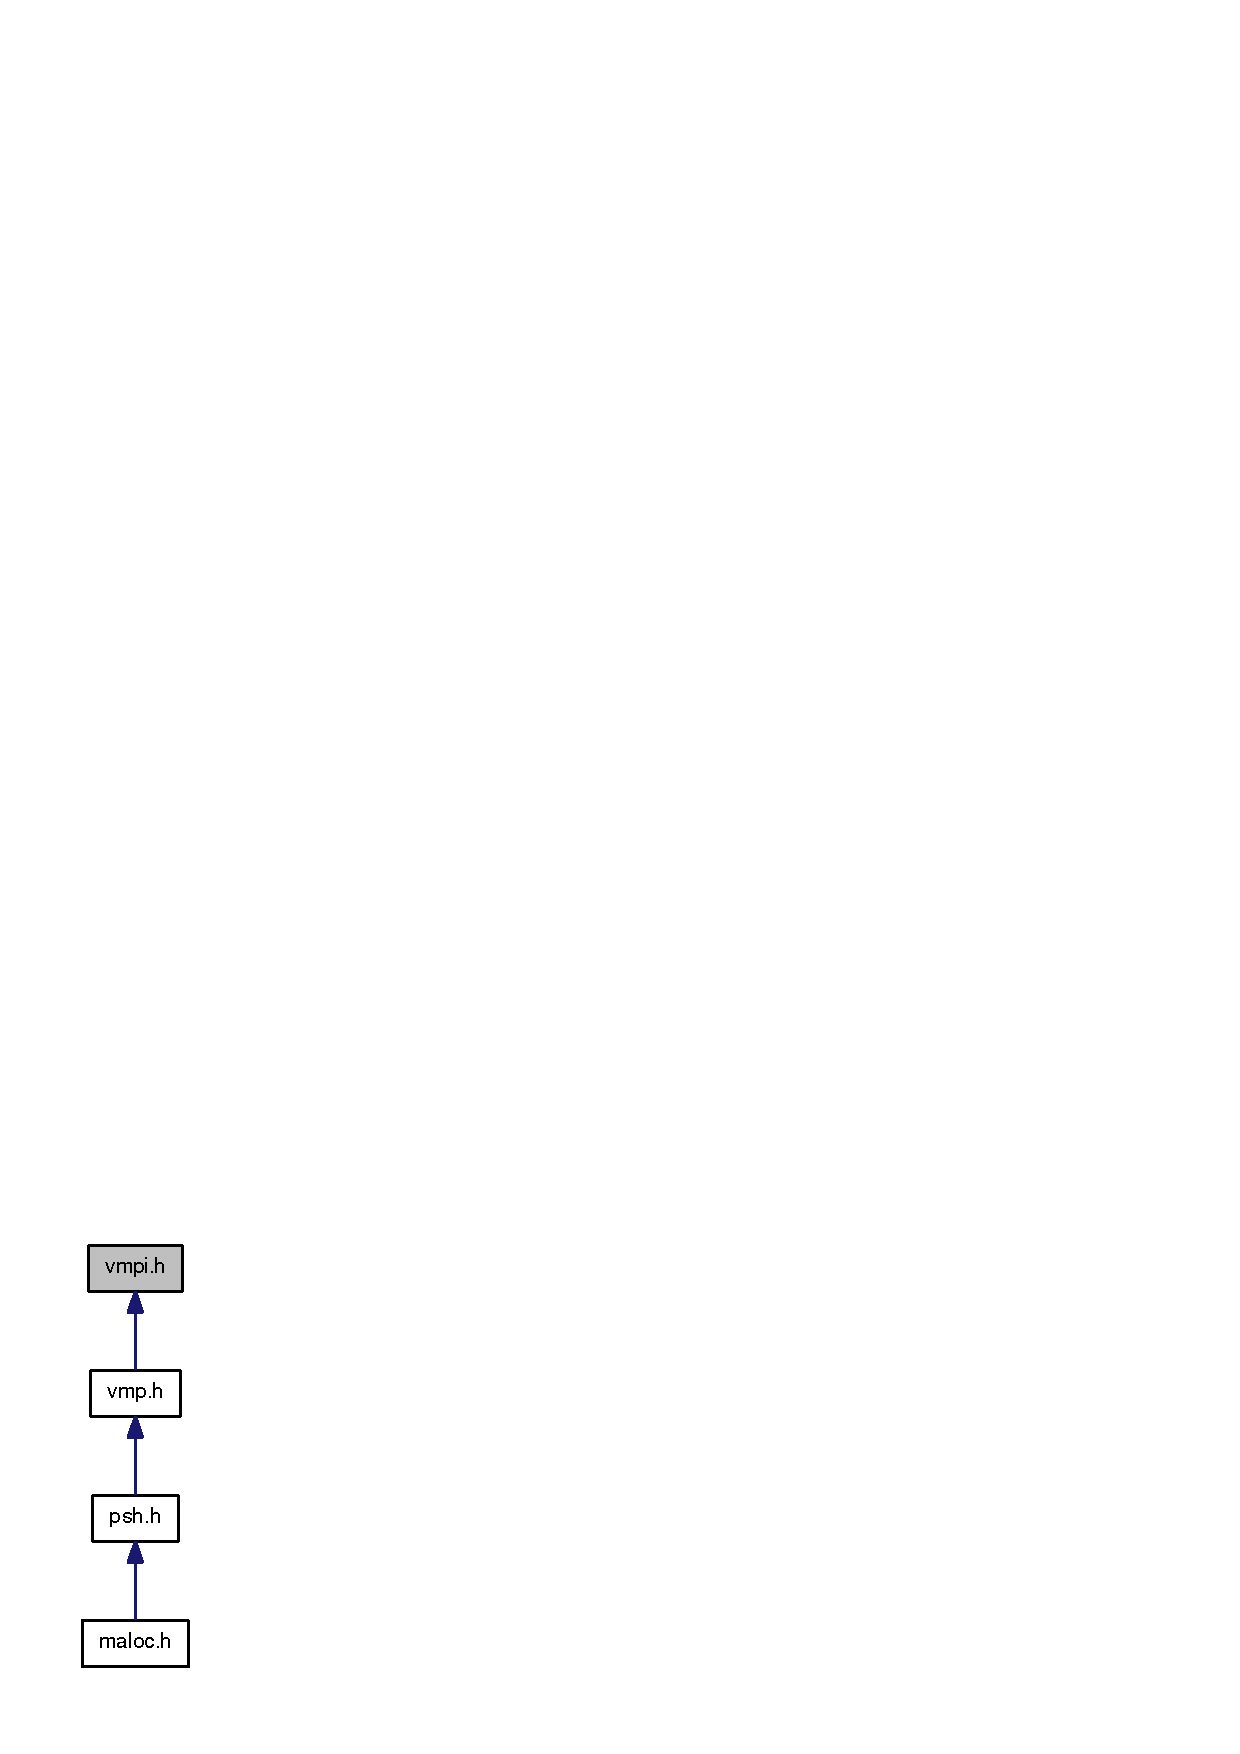
\includegraphics[width=94pt]{a00046}
\end{center}
\end{figure}
\subsection*{Classes}
\begin{DoxyCompactItemize}
\item 
struct {\bf s\+Vmpi}
\begin{DoxyCompactList}\small\item\em Class Vmpi\+: Definition. \end{DoxyCompactList}\end{DoxyCompactItemize}
\subsection*{Typedefs}
\begin{DoxyCompactItemize}
\item 
typedef struct {\bf s\+Vmpi} {\bf Vmpi}
\begin{DoxyCompactList}\small\item\em Declaration of the Vmpi class as the Vmpi structure. \end{DoxyCompactList}\end{DoxyCompactItemize}
\subsection*{Functions}
\begin{DoxyCompactItemize}
\item 
int {\bf Vmpi\+\_\+init} (int $\ast$argc, char $\ast$$\ast$$\ast$argv)
\begin{DoxyCompactList}\small\item\em The Vmp initializer. \end{DoxyCompactList}\item 
int {\bf Vmpi\+\_\+finalize} (void)
\begin{DoxyCompactList}\small\item\em The Vmp finalizer. \end{DoxyCompactList}\item 
{\bf Vmpi} $\ast$ {\bf Vmpi\+\_\+ctor} (void)
\begin{DoxyCompactList}\small\item\em The Vmpi constructor. \end{DoxyCompactList}\item 
void {\bf Vmpi\+\_\+dtor} ({\bf Vmpi} $\ast$$\ast$thee)
\begin{DoxyCompactList}\small\item\em The Vmpi destructor. \end{DoxyCompactList}\item 
int {\bf Vmpi\+\_\+rank} ({\bf Vmpi} $\ast$thee)
\begin{DoxyCompactList}\small\item\em Return my processor I\+D. \end{DoxyCompactList}\item 
int {\bf Vmpi\+\_\+size} ({\bf Vmpi} $\ast$thee)
\begin{DoxyCompactList}\small\item\em Return the number of processors involved. \end{DoxyCompactList}\item 
int {\bf Vmpi\+\_\+barr} ({\bf Vmpi} $\ast$thee)
\begin{DoxyCompactList}\small\item\em An M\+P\+I barrier. \end{DoxyCompactList}\item 
int {\bf Vmpi\+\_\+send} ({\bf Vmpi} $\ast$thee, int des, char $\ast$buf, int bufsize)
\begin{DoxyCompactList}\small\item\em An M\+P\+I blocking send. \end{DoxyCompactList}\item 
int {\bf Vmpi\+\_\+recv} ({\bf Vmpi} $\ast$thee, int src, char $\ast$buf, int bufsize)
\begin{DoxyCompactList}\small\item\em An M\+P\+I blocking receive. \end{DoxyCompactList}\item 
int {\bf Vmpi\+\_\+bcast} ({\bf Vmpi} $\ast$thee, char $\ast$buf, int bufsize)
\begin{DoxyCompactList}\small\item\em An M\+P\+I broadcast. \end{DoxyCompactList}\item 
int {\bf Vmpi\+\_\+reduce} ({\bf Vmpi} $\ast$thee, char $\ast$sbuf, char $\ast$rbuf, int bufsize)
\begin{DoxyCompactList}\small\item\em An M\+P\+I reduce. \end{DoxyCompactList}\item 
int {\bf Vmpi\+\_\+isend} ({\bf Vmpi} $\ast$thee, int des, char $\ast$buf, int bufsize)
\begin{DoxyCompactList}\small\item\em An M\+P\+I non-\/blocking send. \end{DoxyCompactList}\end{DoxyCompactItemize}


\subsection{Detailed Description}
Class Vmpi\+: a Virtual M\+P\+I communication layer object. 

\begin{DoxyAuthor}{Author}
Michael Holst 
\end{DoxyAuthor}
\begin{DoxyNote}{Note}
None 
\end{DoxyNote}
\begin{DoxyVersion}{Version}

\end{DoxyVersion}
\begin{DoxyParagraph}{Id}
\doxyref{vmpi.\+h}{p.}{a00017},v 1.\+29 2010/08/12 05\+:40\+:23 fetk Exp 
\end{DoxyParagraph}


\begin{DoxyAttention}{Attention}
\begin{DoxyVerb}*
* MALOC = < Minimal Abstraction Layer for Object-oriented C >
* Copyright (C) 1994-- Michael Holst
*
* This library is free software; you can redistribute it and/or
* modify it under the terms of the GNU Lesser General Public
* License as published by the Free Software Foundation; either
* version 2.1 of the License, or (at your option) any later version.
*
* This library is distributed in the hope that it will be useful,
* but WITHOUT ANY WARRANTY; without even the implied warranty of
* MERCHANTABILITY or FITNESS FOR A PARTICULAR PURPOSE. See the GNU
* Lesser General Public License for more details.
*
* You should have received a copy of the GNU Lesser General Public
* License along with this library; if not, write to the Free Software
* Foundation, Inc., 59 Temple Place, Suite 330, Boston, MA 02111-1307 USA
* 
*  \end{DoxyVerb}
 
\end{DoxyAttention}

\section{vnm.h File Reference}
\label{a00018}\index{vnm.h@{vnm.h}}


Header file for an ISO C [V]irtual [N]umerical [M]achine.  


{\ttfamily \#include $<$maloc/maloc\_\-base.h$>$}\par
Include dependency graph for vnm.h:
\nopagebreak
\begin{figure}[H]
\begin{center}
\leavevmode
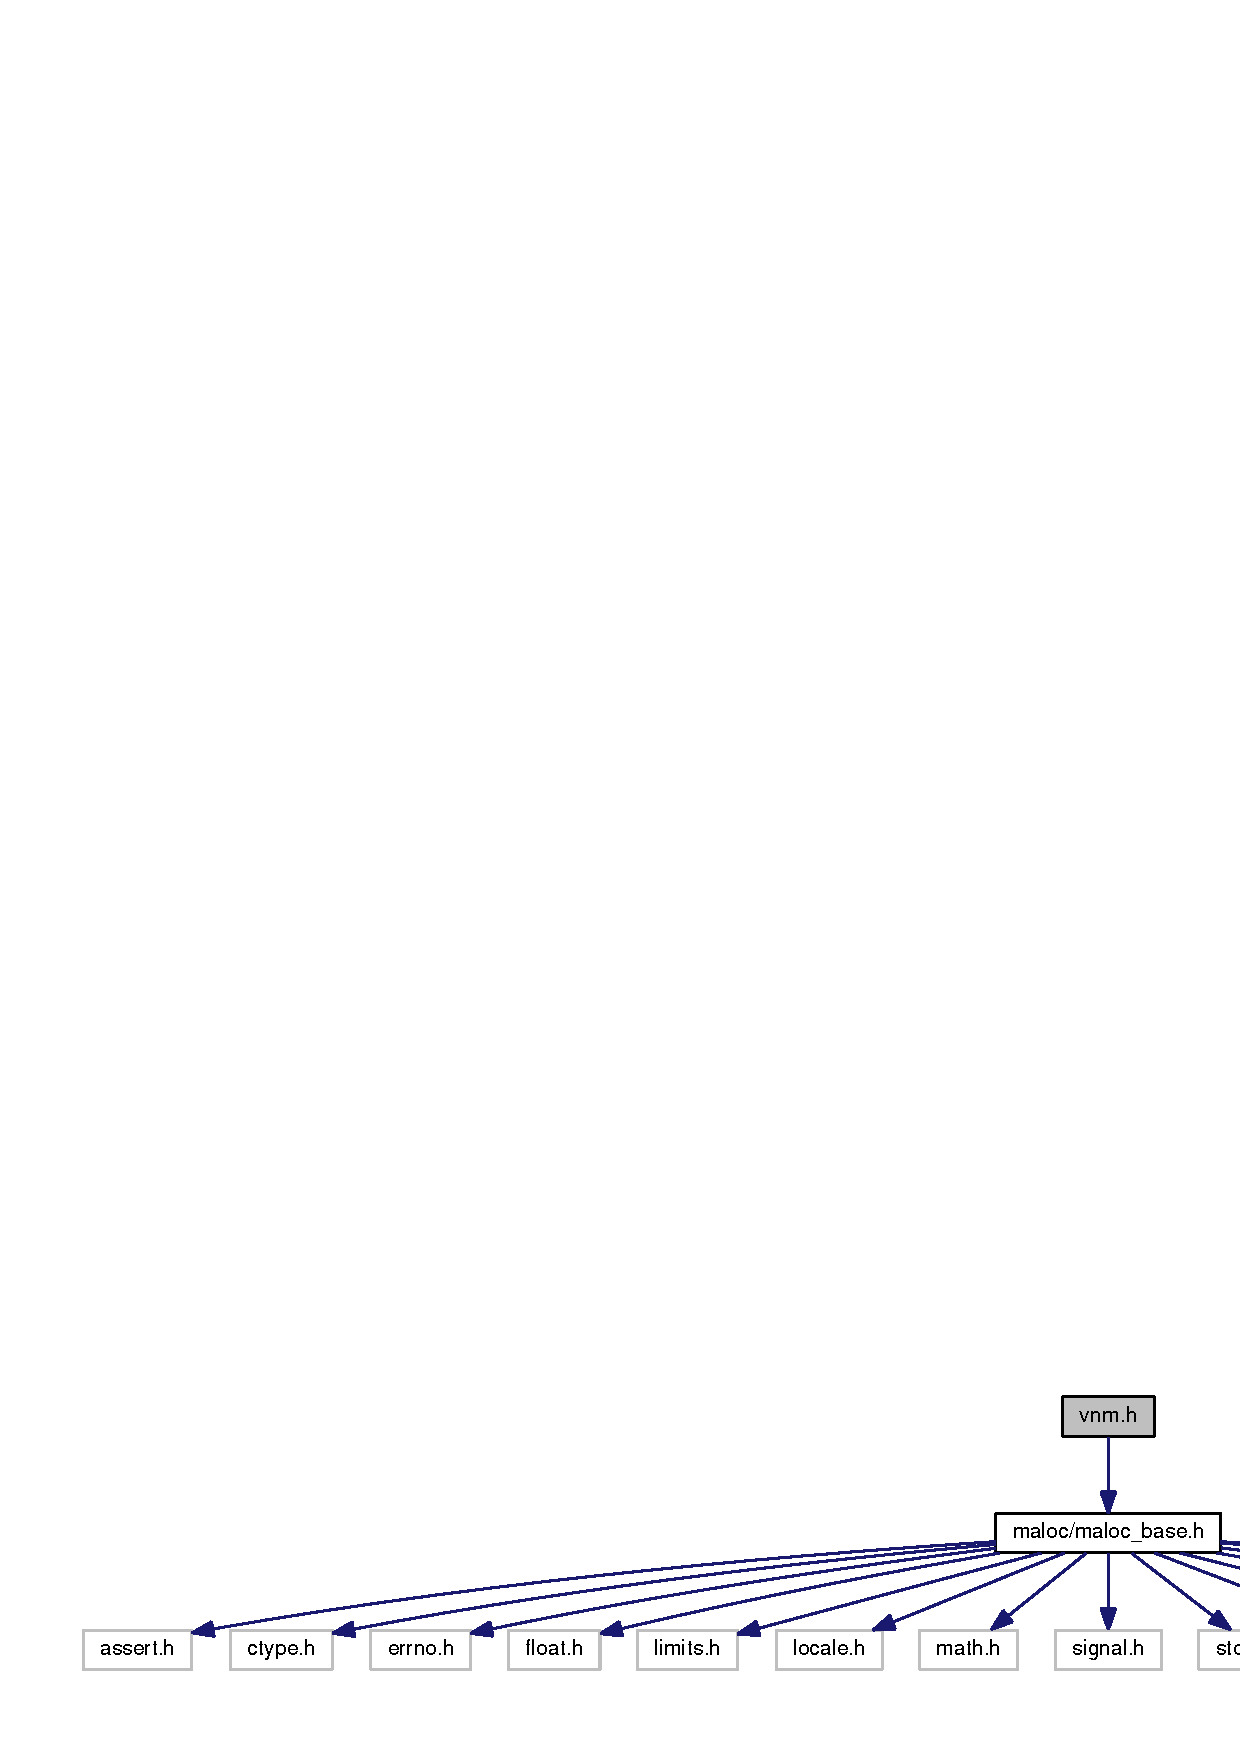
\includegraphics[width=400pt]{a00047}
\end{center}
\end{figure}
This graph shows which files directly or indirectly include this file:
\nopagebreak
\begin{figure}[H]
\begin{center}
\leavevmode
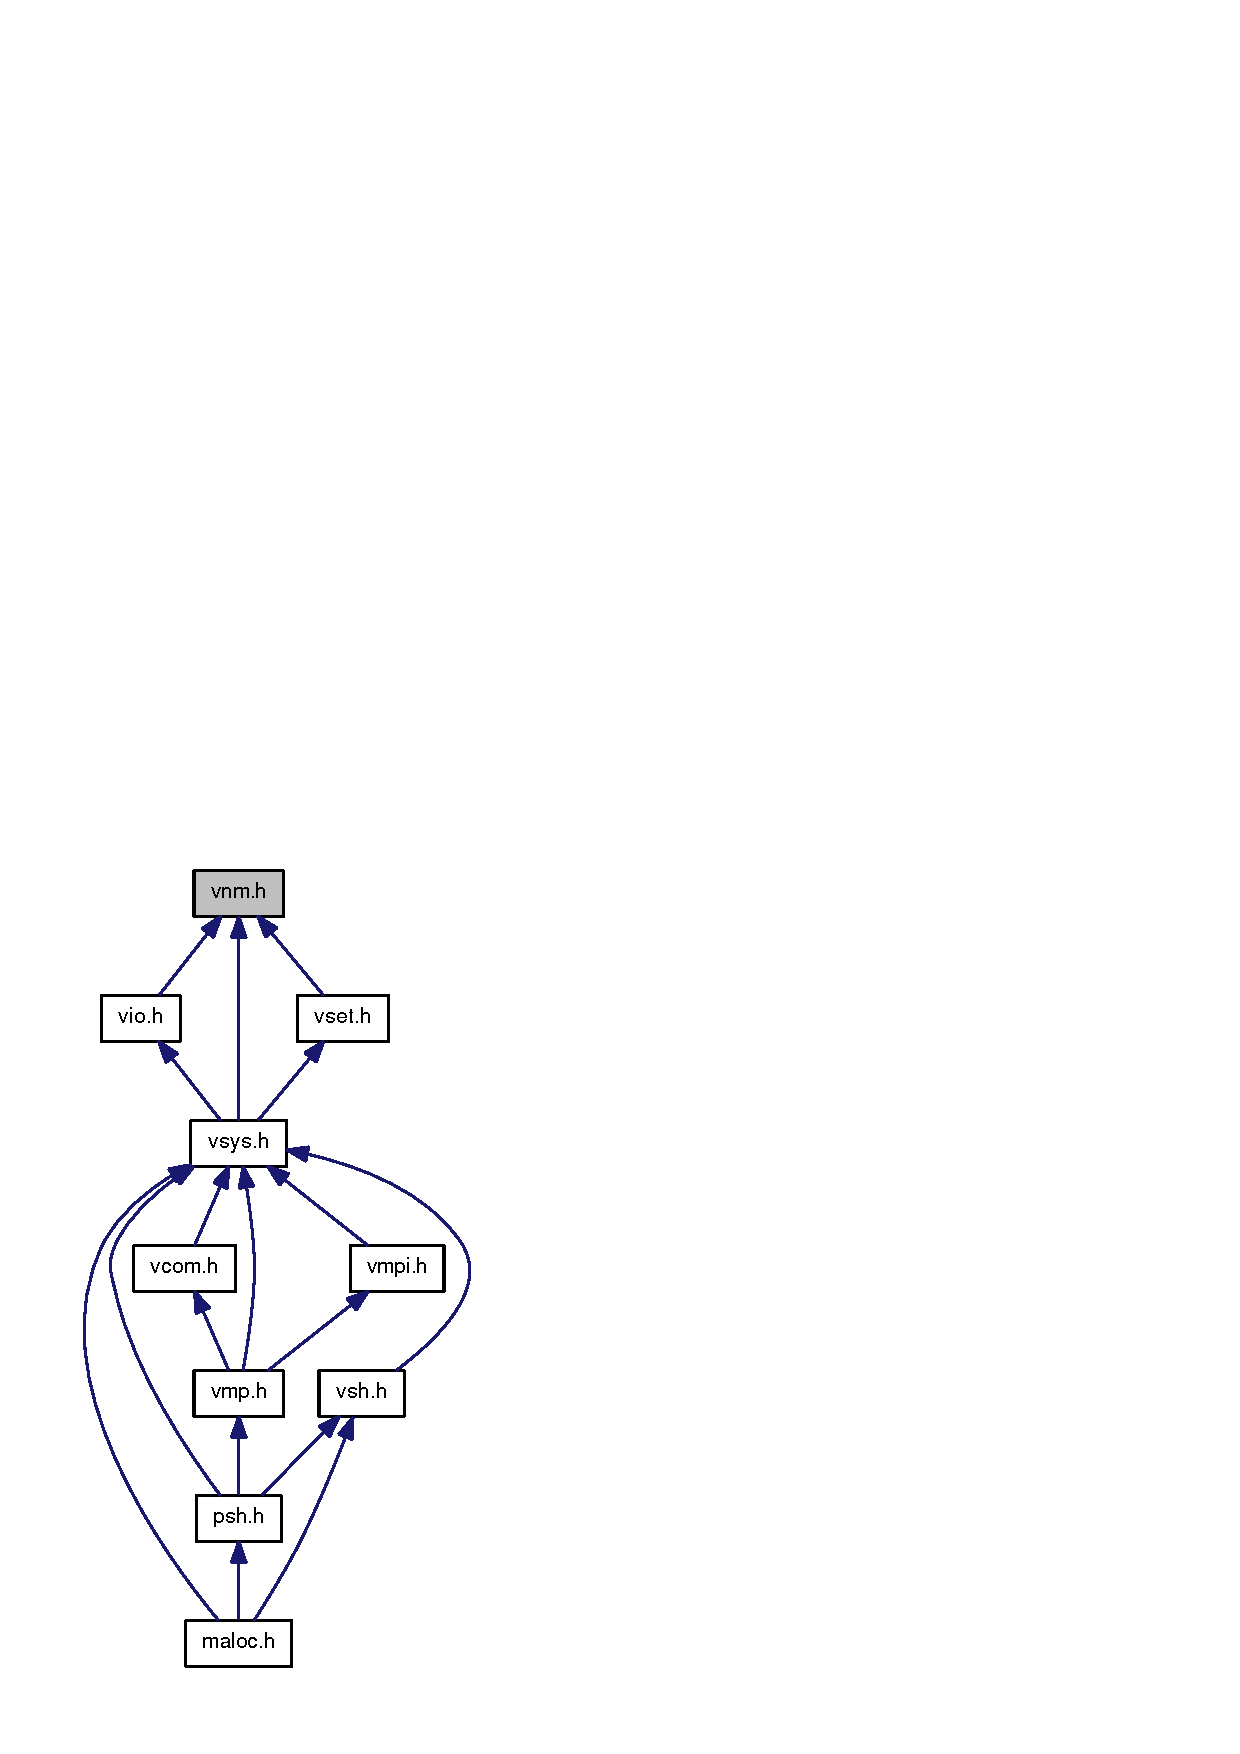
\includegraphics[width=230pt]{a00048}
\end{center}
\end{figure}
\subsection*{Defines}
\begin{DoxyCompactItemize}
\item 
\#define {\bf VPOW\_\-SAFE}(x, y)~(Vnm\_\-powsafe(x,y))
\begin{DoxyCompactList}\small\item\em A safe VPOW function (avoids division by zero). \item\end{DoxyCompactList}\item 
\#define {\bf VTIMERS}~100
\begin{DoxyCompactList}\small\item\em the maiximal timer constant \item\end{DoxyCompactList}\end{DoxyCompactItemize}
\subsection*{Functions}
\begin{DoxyCompactItemize}
\item 
int {\bf Vnm\_\-sigInt} (void)
\begin{DoxyCompactList}\small\item\em Signal and setjmp handling routine. Return the signal interrupt flag. \item\end{DoxyCompactList}\item 
void {\bf Vnm\_\-sigIntSet} (void)
\begin{DoxyCompactList}\small\item\em Signal and setjmp handling routine. Set the signal interrupt flag. \item\end{DoxyCompactList}\item 
void {\bf Vnm\_\-sigIntClear} (void)
\begin{DoxyCompactList}\small\item\em Signal and setjmp handling routine. Clear the signal interrupt flag. \item\end{DoxyCompactList}\item 
int {\bf Vnm\_\-jmpOk} (void)
\begin{DoxyCompactList}\small\item\em Signal and setjmp handling routine. Return the \char`\"{}ok-\/to-\/jump\char`\"{} flag. \item\end{DoxyCompactList}\item 
void {\bf Vnm\_\-jmpOkSet} (void)
\begin{DoxyCompactList}\small\item\em Signal and setjmp handling routine. Set the \char`\"{}okay-\/to-\/jump\char`\"{} flag. \item\end{DoxyCompactList}\item 
void {\bf Vnm\_\-jmpOkClear} (void)
\begin{DoxyCompactList}\small\item\em Signal and setjmp handling routine. Clear the \char`\"{}okay-\/to-\/jump\char`\"{} flag. \item\end{DoxyCompactList}\item 
jmp\_\-buf $\ast$ {\bf Vnm\_\-signalInit} (void)
\begin{DoxyCompactList}\small\item\em Initialize the signal handling data structures. \item\end{DoxyCompactList}\item 
void {\bf Vnm\_\-regHand} (void)
\begin{DoxyCompactList}\small\item\em Register the signal handler with the operating system. \item\end{DoxyCompactList}\item 
void {\bf Vnm\_\-sigHand} (int num)
\begin{DoxyCompactList}\small\item\em Handle events such as SIGINT. We must have first been registered with \char`\"{}Vnm\_\-signalInit\char`\"{}. \item\end{DoxyCompactList}\item 
double {\bf Vnm\_\-powsafe} (double x, double y)
\begin{DoxyCompactList}\small\item\em A safe VPOW function (avoids division by zero). \item\end{DoxyCompactList}\item 
void {\bf Vnm\_\-typeChk} (void)
\begin{DoxyCompactList}\small\item\em Check out the sizes of various datatypes. \item\end{DoxyCompactList}\item 
double {\bf Vnm\_\-epsmac} (void)
\begin{DoxyCompactList}\small\item\em Computes the unit roundoff of the machine in single precision. This is defined as the smallest positive machine number u such that 1.0d0 + u .ne. 1.0d0 (in single precision). \par
\par
 A safe hardcoded machine epsilon as alternative:\par
 double value; \par
 value = 1.0e-\/9; \par
 return value;. \item\end{DoxyCompactList}\item 
int {\bf Vnm\_\-gentokens} (char $\ast$buf, char $\ast$$\ast$argv, const int argvmax, const char $\ast$white, const char $\ast$comment)
\begin{DoxyCompactList}\small\item\em Generate an [argv,argc] pair from a character string \char`\"{}buf\char`\"{} (assumed NULL-\/terminated) in which tokens are separated by whitespace \char`\"{}white\char`\"{} with possible comments \char`\"{}comment\char`\"{} occuring. THE INPUT STRING IS MODIFIED HERE! \item\end{DoxyCompactList}\item 
void {\bf Vnm\_\-tstart} (int timer, const char $\ast$name)
\begin{DoxyCompactList}\small\item\em Starts the timer on the particular machine. \item\end{DoxyCompactList}\item 
void {\bf Vnm\_\-tstop} (int timer, const char $\ast$name)
\begin{DoxyCompactList}\small\item\em Stops the timer on the particular machine. \item\end{DoxyCompactList}\item 
char $\ast$ {\bf Vnm\_\-getuser} (char $\ast$user, int usermax)
\begin{DoxyCompactList}\small\item\em Ask the system for the username. \item\end{DoxyCompactList}\item 
char $\ast$ {\bf Vnm\_\-getos} (char $\ast$os, int osmax)
\begin{DoxyCompactList}\small\item\em Ask the system for the operating system name. \item\end{DoxyCompactList}\item 
char $\ast$ {\bf Vnm\_\-gethost} (char $\ast$host, int hostmax)
\begin{DoxyCompactList}\small\item\em Ask the system for the hostname. \item\end{DoxyCompactList}\item 
char $\ast$ {\bf Vnm\_\-gethome} (char $\ast$path, int pathmax)
\begin{DoxyCompactList}\small\item\em Ask the system for the home directory. \item\end{DoxyCompactList}\item 
char $\ast$ {\bf Vnm\_\-getcwd} (char $\ast$path, int pathmax)
\begin{DoxyCompactList}\small\item\em Ask the system for the current working directory. \item\end{DoxyCompactList}\item 
int {\bf Vnm\_\-chdir} (const char $\ast$path)
\begin{DoxyCompactList}\small\item\em Interact with the system to change the working directory. \item\end{DoxyCompactList}\item 
int {\bf Vnm\_\-mkdir} (const char $\ast$path)
\begin{DoxyCompactList}\small\item\em Interact with the system to make a new directory. \item\end{DoxyCompactList}\item 
int {\bf Vnm\_\-system} (const char $\ast$cmd)
\begin{DoxyCompactList}\small\item\em An improved ANSI-\/C \char`\"{}system\char`\"{} call. \item\end{DoxyCompactList}\item 
int {\bf Vnm\_\-systemBack} (const char $\ast$cmd)
\begin{DoxyCompactList}\small\item\em A background variant of the ANSI-\/C \char`\"{}system\char`\"{} call. \item\end{DoxyCompactList}\item 
int {\bf Vnm\_\-systemKill} (const char $\ast$cmd)
\begin{DoxyCompactList}\small\item\em Something like a UNIX \char`\"{}killall\char`\"{} call. \item\end{DoxyCompactList}\item 
int {\bf Vnm\_\-exec} (int argc, char $\ast$$\ast$argv)
\begin{DoxyCompactList}\small\item\em An improved UNIX \char`\"{}exec\char`\"{} call. This routine does not return except on error. \item\end{DoxyCompactList}\item 
void {\bf Vnm\_\-sleep} (int nusecs)
\begin{DoxyCompactList}\small\item\em Implement a sleep function with microsecond resolution. \item\end{DoxyCompactList}\item 
int {\bf Vnm\_\-ioTag} (void)
\begin{DoxyCompactList}\small\item\em Return my I/O tag. \item\end{DoxyCompactList}\item 
int {\bf Vnm\_\-nTags} (void)
\begin{DoxyCompactList}\small\item\em Return the total number of tags. \item\end{DoxyCompactList}\item 
void {\bf Vnm\_\-setIoTag} (int myTag, int numTags)
\begin{DoxyCompactList}\small\item\em Set my id. \item\end{DoxyCompactList}\item 
FILE $\ast$ {\bf Vnm\_\-open} (const int unit)
\begin{DoxyCompactList}\small\item\em Open an I/O console. \item\end{DoxyCompactList}\item 
int {\bf Vnm\_\-close} (const int unit)
\begin{DoxyCompactList}\small\item\em Close an I/O console. We MUST NOT use VASSERT (or Vnm\_\-print!) in this routine. \item\end{DoxyCompactList}\item 
void {\bf Vnm\_\-flush} (const int unit)
\begin{DoxyCompactList}\small\item\em Attempt to flush the specified i/o stream. We MUST NOT use VASSERT (or Vnm\_\-print!) in this routine. \item\end{DoxyCompactList}\item 
void {\bf Vnm\_\-redirect} (const int flag)
\begin{DoxyCompactList}\small\item\em Set/unset the redirect flag for UNIT zero. When redirected, I/O goes to the {\tt file:} \$\{MCSH\_\-HOME\}/io.mc. We MUST NOT use VASSERT (or Vnm\_\-print!) in this routine. \item\end{DoxyCompactList}\item 
void {\bf Vnm\_\-print} (const int unit, const char $\ast$format,...)
\begin{DoxyCompactList}\small\item\em External interface to the console i/o routine. We MUST NOT use VASSERT (or Vnm\_\-print!) in this routine. \item\end{DoxyCompactList}\item 
void {\bf Vnm\_\-tprint} (const int unit, const char $\ast$format,...)
\begin{DoxyCompactList}\small\item\em Add our ioTag to Vnm\_\-print output. We MUST NOT use VASSERT (or Vnm\_\-print!) in this routine. \item\end{DoxyCompactList}\item 
void {\bf Vnm\_\-qsort} (int $\ast$u, int size)
\begin{DoxyCompactList}\small\item\em Front-\/end to quick sort integer array from [-\/large] to [+large]. \item\end{DoxyCompactList}\item 
void {\bf Vnm\_\-qsortOrd} (int $\ast$u, int $\ast$ord, int size)
\begin{DoxyCompactList}\small\item\em Front-\/end to quick sort integer array from [-\/large] to [+large]. \item\end{DoxyCompactList}\item 
void {\bf Vnm\_\-dqsort} (double $\ast$u, int size)
\begin{DoxyCompactList}\small\item\em Front-\/end to quick sort integer array from [-\/large] to [+large]. \item\end{DoxyCompactList}\item 
void {\bf Vnm\_\-dqsortOrd} (double $\ast$u, int $\ast$ord, int size)
\begin{DoxyCompactList}\small\item\em Front-\/end to quick sort integer array from [-\/large] to [+large]. \item\end{DoxyCompactList}\end{DoxyCompactItemize}


\subsection{Detailed Description}
Header file for an ISO C [V]irtual [N]umerical [M]achine. \begin{DoxyAuthor}{Author}
Michael Holst 
\end{DoxyAuthor}
\begin{DoxyNote}{Note}
None 
\end{DoxyNote}
\begin{DoxyVersion}{Version}

\end{DoxyVersion}
\begin{DoxyParagraph}{Id:}
\doxyref{vnm.h}{p.}{a00018},v 1.22 2010/08/12 05:40:36 fetk Exp 
\end{DoxyParagraph}


\begin{DoxyAttention}{Attention}
\begin{DoxyVerb}
 *
 * MALOC = < Minimal Abstraction Layer for Object-oriented C >
 * Copyright (C) 1994-- Michael Holst
 *
 * This library is free software; you can redistribute it and/or
 * modify it under the terms of the GNU Lesser General Public
 * License as published by the Free Software Foundation; either
 * version 2.1 of the License, or (at your option) any later version.
 *
 * This library is distributed in the hope that it will be useful,
 * but WITHOUT ANY WARRANTY; without even the implied warranty of
 * MERCHANTABILITY or FITNESS FOR A PARTICULAR PURPOSE. See the GNU
 * Lesser General Public License for more details.
 *
 * You should have received a copy of the GNU Lesser General Public
 * License along with this library; if not, write to the Free Software
 * Foundation, Inc., 59 Temple Place, Suite 330, Boston, MA 02111-1307 USA
 * 
 *  \end{DoxyVerb}
 
\end{DoxyAttention}


\subsection{Define Documentation}
\index{vnm.h@{vnm.h}!VPOW\_\-SAFE@{VPOW\_\-SAFE}}
\index{VPOW\_\-SAFE@{VPOW\_\-SAFE}!vnm.h@{vnm.h}}
\subsubsection[{VPOW\_\-SAFE}]{\setlength{\rightskip}{0pt plus 5cm}\#define VPOW\_\-SAFE(
\begin{DoxyParamCaption}
\item[{}]{x, }
\item[{}]{y}
\end{DoxyParamCaption}
)~(Vnm\_\-powsafe(x,y))}\label{a00018_ad7c91b8e4ceddff38851300876c7c9e7}


A safe VPOW function (avoids division by zero). 

\begin{DoxyNote}{Note}
Useful constants and functions (timers, epsilon, token generators, i/o) 
\end{DoxyNote}
\index{vnm.h@{vnm.h}!VTIMERS@{VTIMERS}}
\index{VTIMERS@{VTIMERS}!vnm.h@{vnm.h}}
\subsubsection[{VTIMERS}]{\setlength{\rightskip}{0pt plus 5cm}\#define VTIMERS~100}\label{a00018_adff08ccefac6ec8e551662478f350e7f}


the maiximal timer constant 

\begin{DoxyNote}{Note}
Useful constants and functions (timers, epsilon, token generators, i/o) 
\end{DoxyNote}


\subsection{Function Documentation}
\index{vnm.h@{vnm.h}!Vnm\_\-chdir@{Vnm\_\-chdir}}
\index{Vnm\_\-chdir@{Vnm\_\-chdir}!vnm.h@{vnm.h}}
\subsubsection[{Vnm\_\-chdir}]{\setlength{\rightskip}{0pt plus 5cm}int Vnm\_\-chdir (
\begin{DoxyParamCaption}
\item[{const char $\ast$}]{ path}
\end{DoxyParamCaption}
)}\label{a00018_aae7852bc441c93b9dd7969d8b7c4b515}


Interact with the system to change the working directory. 

\begin{DoxyAuthor}{Author}
Michael Holst 
\end{DoxyAuthor}
\begin{DoxyNote}{Note}
Useful constants and functions (timers, epsilon, token generators, i/o) 
\end{DoxyNote}
\begin{DoxyReturn}{Returns}
Success enumeration 
\end{DoxyReturn}

\begin{DoxyParams}{Parameters}
\item[{\em path}]Pointer to the path \end{DoxyParams}
\index{vnm.h@{vnm.h}!Vnm\_\-close@{Vnm\_\-close}}
\index{Vnm\_\-close@{Vnm\_\-close}!vnm.h@{vnm.h}}
\subsubsection[{Vnm\_\-close}]{\setlength{\rightskip}{0pt plus 5cm}int Vnm\_\-close (
\begin{DoxyParamCaption}
\item[{const int}]{ unit}
\end{DoxyParamCaption}
)}\label{a00018_a0865f47c73cd78d4abcdc86027b3fbbd}


Close an I/O console. We MUST NOT use VASSERT (or Vnm\_\-print!) in this routine. 

\begin{DoxyAuthor}{Author}
Michael Holst 
\end{DoxyAuthor}
\begin{DoxyNote}{Note}
Useful constants and functions (timers, epsilon, token generators, i/o) 
\end{DoxyNote}
\begin{DoxyReturn}{Returns}
Success enumeration 
\end{DoxyReturn}

\begin{DoxyParams}{Parameters}
\item[{\em unit}]index for the file unit \end{DoxyParams}
\index{vnm.h@{vnm.h}!Vnm\_\-dqsort@{Vnm\_\-dqsort}}
\index{Vnm\_\-dqsort@{Vnm\_\-dqsort}!vnm.h@{vnm.h}}
\subsubsection[{Vnm\_\-dqsort}]{\setlength{\rightskip}{0pt plus 5cm}void Vnm\_\-dqsort (
\begin{DoxyParamCaption}
\item[{double $\ast$}]{ u, }
\item[{int}]{ size}
\end{DoxyParamCaption}
)}\label{a00018_af5dd29bb1fb767ab5cd50a16115c90e2}


Front-\/end to quick sort integer array from [-\/large] to [+large]. 

\begin{DoxyAuthor}{Author}
Michael Holst 
\end{DoxyAuthor}
\begin{DoxyNote}{Note}
Useful constants and functions (timers, epsilon, token generators, i/o) 
\end{DoxyNote}
\begin{DoxyReturn}{Returns}
None 
\end{DoxyReturn}

\begin{DoxyParams}{Parameters}
\item[{\em u}]Pointer to quick sort integer array \item[{\em size}]size of the integer array \end{DoxyParams}
\index{vnm.h@{vnm.h}!Vnm\_\-dqsortOrd@{Vnm\_\-dqsortOrd}}
\index{Vnm\_\-dqsortOrd@{Vnm\_\-dqsortOrd}!vnm.h@{vnm.h}}
\subsubsection[{Vnm\_\-dqsortOrd}]{\setlength{\rightskip}{0pt plus 5cm}void Vnm\_\-dqsortOrd (
\begin{DoxyParamCaption}
\item[{double $\ast$}]{ u, }
\item[{int $\ast$}]{ ord, }
\item[{int}]{ size}
\end{DoxyParamCaption}
)}\label{a00018_a77193dca4dcddfd1ef609f2c50e39a45}


Front-\/end to quick sort integer array from [-\/large] to [+large]. 

\begin{DoxyAuthor}{Author}
Michael Holst 
\end{DoxyAuthor}
\begin{DoxyNote}{Note}
Useful constants and functions (timers, epsilon, token generators, i/o) 
\end{DoxyNote}
\begin{DoxyReturn}{Returns}
None 
\end{DoxyReturn}

\begin{DoxyParams}{Parameters}
\item[{\em u}]Pointer to quick sort integer array \item[{\em ord}]Pointer to reordered array \item[{\em size}]size of the integer array \end{DoxyParams}
\index{vnm.h@{vnm.h}!Vnm\_\-epsmac@{Vnm\_\-epsmac}}
\index{Vnm\_\-epsmac@{Vnm\_\-epsmac}!vnm.h@{vnm.h}}
\subsubsection[{Vnm\_\-epsmac}]{\setlength{\rightskip}{0pt plus 5cm}double Vnm\_\-epsmac (
\begin{DoxyParamCaption}
\item[{void}]{}
\end{DoxyParamCaption}
)}\label{a00018_ac0948dac8295ff4702a3d15b72920823}


Computes the unit roundoff of the machine in single precision. This is defined as the smallest positive machine number u such that 1.0d0 + u .ne. 1.0d0 (in single precision). \par
\par
 A safe hardcoded machine epsilon as alternative:\par
 double value; \par
 value = 1.0e-\/9; \par
 return value;. 

\begin{DoxyAuthor}{Author}
Michael Holst 
\end{DoxyAuthor}
\begin{DoxyNote}{Note}
Useful constants and functions (timers, epsilon, token generators, i/o) 
\end{DoxyNote}
\begin{DoxyReturn}{Returns}
the unit roundoff of the machine in single precision. 
\end{DoxyReturn}
\index{vnm.h@{vnm.h}!Vnm\_\-exec@{Vnm\_\-exec}}
\index{Vnm\_\-exec@{Vnm\_\-exec}!vnm.h@{vnm.h}}
\subsubsection[{Vnm\_\-exec}]{\setlength{\rightskip}{0pt plus 5cm}int Vnm\_\-exec (
\begin{DoxyParamCaption}
\item[{int}]{ argc, }
\item[{char $\ast$$\ast$}]{ argv}
\end{DoxyParamCaption}
)}\label{a00018_a754abd42c8c75dcc3a092fda5700c44b}


An improved UNIX \char`\"{}exec\char`\"{} call. This routine does not return except on error. 

\begin{DoxyAuthor}{Author}
Michael Holst 
\end{DoxyAuthor}
\begin{DoxyNote}{Note}
Useful constants and functions (timers, epsilon, token generators, i/o) 
\end{DoxyNote}
\begin{DoxyReturn}{Returns}
no return except on error 
\end{DoxyReturn}

\begin{DoxyParams}{Parameters}
\item[{\em argc}]number of the command line arguments \item[{\em argv}]the command line arguments \end{DoxyParams}
\index{vnm.h@{vnm.h}!Vnm\_\-flush@{Vnm\_\-flush}}
\index{Vnm\_\-flush@{Vnm\_\-flush}!vnm.h@{vnm.h}}
\subsubsection[{Vnm\_\-flush}]{\setlength{\rightskip}{0pt plus 5cm}void Vnm\_\-flush (
\begin{DoxyParamCaption}
\item[{const int}]{ unit}
\end{DoxyParamCaption}
)}\label{a00018_a6eed22efc46e1bfbd34b54db20422cc6}


Attempt to flush the specified i/o stream. We MUST NOT use VASSERT (or Vnm\_\-print!) in this routine. 

\begin{DoxyAuthor}{Author}
Michael Holst 
\end{DoxyAuthor}
\begin{DoxyNote}{Note}
Useful constants and functions (timers, epsilon, token generators, i/o) 
\end{DoxyNote}
\begin{DoxyReturn}{Returns}
None 
\end{DoxyReturn}

\begin{DoxyParams}{Parameters}
\item[{\em unit}]index for the file unit \end{DoxyParams}
\index{vnm.h@{vnm.h}!Vnm\_\-gentokens@{Vnm\_\-gentokens}}
\index{Vnm\_\-gentokens@{Vnm\_\-gentokens}!vnm.h@{vnm.h}}
\subsubsection[{Vnm\_\-gentokens}]{\setlength{\rightskip}{0pt plus 5cm}int Vnm\_\-gentokens (
\begin{DoxyParamCaption}
\item[{char $\ast$}]{ buf, }
\item[{char $\ast$$\ast$}]{ argv, }
\item[{const int}]{ argvmax, }
\item[{const char $\ast$}]{ white, }
\item[{const char $\ast$}]{ comment}
\end{DoxyParamCaption}
)}\label{a00018_ac4ab27601589fe7256bf75c9b642fadd}


Generate an [argv,argc] pair from a character string \char`\"{}buf\char`\"{} (assumed NULL-\/terminated) in which tokens are separated by whitespace \char`\"{}white\char`\"{} with possible comments \char`\"{}comment\char`\"{} occuring. THE INPUT STRING IS MODIFIED HERE! 

\begin{DoxyAuthor}{Author}
Michael Holst 
\end{DoxyAuthor}
\begin{DoxyNote}{Note}
Useful constants and functions (timers, epsilon, token generators, i/o)\par
\par
 Again, the input string \char`\"{}buf\char`\"{} IS MODIFIED; white space characters (defined in the input string \char`\"{}white\char`\"{}) are replaced by the NULL character '$\backslash$0'. The output \char`\"{}argv\char`\"{} is simply a list of pointers to the start of the tokens in \char`\"{}buf\char`\"{}, which are NULL-\/terminated after we replace the white space with NULLs. \par
\par
 We follow convention and \char`\"{}NULL\char`\"{}-\/terminate \char`\"{}argv\char`\"{} by setting the pointer following the last token to \char`\"{}VNULL\char`\"{}. The return value is \char`\"{}argc\char`\"{}, the number of tokens found (not including the terminating NULL pointer). For safety you must pass in the maximal length of argv in the parameter \char`\"{}argvmax\char`\"{}.\par
\par
 If we encounter a token which begins with a comment character (defined in the input string \char`\"{}comment\char`\"{}), then we ignore the rest of the tokens in the input buffer \char`\"{}buf\char`\"{}. This is suitable for parsing shell languages such as sh/ksh/bash which have comments that start with e.g. \char`\"{}\#\char`\"{} and continue until a newline.\par
\par
 We DO NOT use the C library function strtok in this routine. (There are some bad implementations of strtok around apparently; the internal state variables maintained by strtok can get very messed up if you use strtok in multiple places in a code.) 
\end{DoxyNote}
\begin{DoxyReturn}{Returns}
number of tokens 
\end{DoxyReturn}

\begin{DoxyParams}{Parameters}
\item[{\em buf}]buffer containing message \item[{\em argv}]the command line arguments \item[{\em argvmax}]maximal number of the command line arguments \item[{\em white}]Pointer to the input string \item[{\em comment}]token which begins with a comment character \end{DoxyParams}
\index{vnm.h@{vnm.h}!Vnm\_\-getcwd@{Vnm\_\-getcwd}}
\index{Vnm\_\-getcwd@{Vnm\_\-getcwd}!vnm.h@{vnm.h}}
\subsubsection[{Vnm\_\-getcwd}]{\setlength{\rightskip}{0pt plus 5cm}char$\ast$ Vnm\_\-getcwd (
\begin{DoxyParamCaption}
\item[{char $\ast$}]{ path, }
\item[{int}]{ pathmax}
\end{DoxyParamCaption}
)}\label{a00018_a2a4f1dc46ffecd87eb268ea9194bad03}


Ask the system for the current working directory. 

\begin{DoxyAuthor}{Author}
Michael Holst 
\end{DoxyAuthor}
\begin{DoxyNote}{Note}
Useful constants and functions (timers, epsilon, token generators, i/o)\par
\par
 Consider it an error if we can't return something useful; therefore we will VASSERT(path!=VNULL) before returning. \par
\par
 Note that unlike Vnm\_\-gethome, a call to Vnm\_\-getcwd returns the current directory, possibly modified from call to call.\par
\par
 I.e., calls to Vnm\_\-chdir can change the current working directory; Vnm\_\-getcwd returns the current directory, whatever that might be. 
\end{DoxyNote}
\begin{DoxyReturn}{Returns}
the current working directory 
\end{DoxyReturn}

\begin{DoxyParams}{Parameters}
\item[{\em path}]Pointer to the path \item[{\em pathmax}]index for the size of path \end{DoxyParams}
\index{vnm.h@{vnm.h}!Vnm\_\-gethome@{Vnm\_\-gethome}}
\index{Vnm\_\-gethome@{Vnm\_\-gethome}!vnm.h@{vnm.h}}
\subsubsection[{Vnm\_\-gethome}]{\setlength{\rightskip}{0pt plus 5cm}char$\ast$ Vnm\_\-gethome (
\begin{DoxyParamCaption}
\item[{char $\ast$}]{ path, }
\item[{int}]{ pathmax}
\end{DoxyParamCaption}
)}\label{a00018_a91487bd659791ee680b0b6a4650d3bb1}


Ask the system for the home directory. 

= \begin{DoxyAuthor}{Author}
Michael Holst 
\end{DoxyAuthor}
\begin{DoxyNote}{Note}
Useful constants and functions (timers, epsilon, token generators, i/o)\par
\par
 The following preference order is used to set the home directory: \par
\par
 MCSH\_\-HOME (the user must define this in his environment) \par
 CWD (always defined as the current working directory) \par
\par
 We consider it an error if we can't return something useful; therefore we will VASSERT(path!=VNULL) before returning.\par
\par
 We settle on a home directory the first time we are called, and then we simply return this fixed home directory forever. In other words, the first call to Vnm\_\-gethome, regardless of who makes the call, establishes the home directory for everyone else (as long as everyone goes through Vnm\_\-gethome!). 
\end{DoxyNote}
\begin{DoxyReturn}{Returns}
the home directory 
\end{DoxyReturn}

\begin{DoxyParams}{Parameters}
\item[{\em path}]Pointer to the path \item[{\em pathmax}]index for the size of path \end{DoxyParams}
\index{vnm.h@{vnm.h}!Vnm\_\-gethost@{Vnm\_\-gethost}}
\index{Vnm\_\-gethost@{Vnm\_\-gethost}!vnm.h@{vnm.h}}
\subsubsection[{Vnm\_\-gethost}]{\setlength{\rightskip}{0pt plus 5cm}char$\ast$ Vnm\_\-gethost (
\begin{DoxyParamCaption}
\item[{char $\ast$}]{ host, }
\item[{int}]{ hostmax}
\end{DoxyParamCaption}
)}\label{a00018_afd1fc5ab933eab6ea1b28935c37bcad9}


Ask the system for the hostname. 

\begin{DoxyAuthor}{Author}
Michael Holst 
\end{DoxyAuthor}
\begin{DoxyNote}{Note}
Useful constants and functions (timers, epsilon, token generators, i/o) 
\end{DoxyNote}
\begin{DoxyReturn}{Returns}
the hostname 
\end{DoxyReturn}

\begin{DoxyParams}{Parameters}
\item[{\em host}]Pointer to the hostname. \item[{\em hostmax}]index for maximal size of host name \end{DoxyParams}
\index{vnm.h@{vnm.h}!Vnm\_\-getos@{Vnm\_\-getos}}
\index{Vnm\_\-getos@{Vnm\_\-getos}!vnm.h@{vnm.h}}
\subsubsection[{Vnm\_\-getos}]{\setlength{\rightskip}{0pt plus 5cm}char$\ast$ Vnm\_\-getos (
\begin{DoxyParamCaption}
\item[{char $\ast$}]{ os, }
\item[{int}]{ osmax}
\end{DoxyParamCaption}
)}\label{a00018_a6485dca93aa622f7291d49dbec989b7b}


Ask the system for the operating system name. 

\begin{DoxyAuthor}{Author}
Michael Holst 
\end{DoxyAuthor}
\begin{DoxyNote}{Note}
Useful constants and functions (timers, epsilon, token generators, i/o) 
\end{DoxyNote}
\begin{DoxyReturn}{Returns}
the operating system name 
\end{DoxyReturn}

\begin{DoxyParams}{Parameters}
\item[{\em os}]Pointer to the OS type \item[{\em osmax}]index for maximal size of OS name \end{DoxyParams}
\index{vnm.h@{vnm.h}!Vnm\_\-getuser@{Vnm\_\-getuser}}
\index{Vnm\_\-getuser@{Vnm\_\-getuser}!vnm.h@{vnm.h}}
\subsubsection[{Vnm\_\-getuser}]{\setlength{\rightskip}{0pt plus 5cm}char$\ast$ Vnm\_\-getuser (
\begin{DoxyParamCaption}
\item[{char $\ast$}]{ user, }
\item[{int}]{ usermax}
\end{DoxyParamCaption}
)}\label{a00018_a688a4351e45ae4607d7c4313dd738eb0}


Ask the system for the username. 

\begin{DoxyAuthor}{Author}
Michael Holst 
\end{DoxyAuthor}
\begin{DoxyNote}{Note}
Useful constants and functions (timers, epsilon, token generators, i/o) 
\end{DoxyNote}
\begin{DoxyReturn}{Returns}
the username of the system 
\end{DoxyReturn}

\begin{DoxyParams}{Parameters}
\item[{\em user}]Pointer to the username of the system \item[{\em usermax}]index for maximal size of user name \end{DoxyParams}
\index{vnm.h@{vnm.h}!Vnm\_\-ioTag@{Vnm\_\-ioTag}}
\index{Vnm\_\-ioTag@{Vnm\_\-ioTag}!vnm.h@{vnm.h}}
\subsubsection[{Vnm\_\-ioTag}]{\setlength{\rightskip}{0pt plus 5cm}int Vnm\_\-ioTag (
\begin{DoxyParamCaption}
\item[{void}]{}
\end{DoxyParamCaption}
)}\label{a00018_a1f1c6ac80fc4f4cb4a8524d98d7d2458}


Return my I/O tag. 

\begin{DoxyAuthor}{Author}
Michael Holst 
\end{DoxyAuthor}
\begin{DoxyNote}{Note}
Useful constants and functions (timers, epsilon, token generators, i/o) 
\end{DoxyNote}
\begin{DoxyReturn}{Returns}
my I/O tag. 
\end{DoxyReturn}
\index{vnm.h@{vnm.h}!Vnm\_\-jmpOk@{Vnm\_\-jmpOk}}
\index{Vnm\_\-jmpOk@{Vnm\_\-jmpOk}!vnm.h@{vnm.h}}
\subsubsection[{Vnm\_\-jmpOk}]{\setlength{\rightskip}{0pt plus 5cm}int Vnm\_\-jmpOk (
\begin{DoxyParamCaption}
\item[{void}]{}
\end{DoxyParamCaption}
)}\label{a00018_aaf928e6a4a6022b02a93fb0b33e3799b}


Signal and setjmp handling routine. Return the \char`\"{}ok-\/to-\/jump\char`\"{} flag. 

\begin{DoxyAuthor}{Author}
Michael Holst 
\end{DoxyAuthor}
\begin{DoxyNote}{Note}
Useful constants and functions (timers, epsilon, token generators, i/o) 
\end{DoxyNote}
\begin{DoxyReturn}{Returns}
\char`\"{}ok-\/to-\/jump\char`\"{} flag. 
\end{DoxyReturn}
\index{vnm.h@{vnm.h}!Vnm\_\-jmpOkClear@{Vnm\_\-jmpOkClear}}
\index{Vnm\_\-jmpOkClear@{Vnm\_\-jmpOkClear}!vnm.h@{vnm.h}}
\subsubsection[{Vnm\_\-jmpOkClear}]{\setlength{\rightskip}{0pt plus 5cm}void Vnm\_\-jmpOkClear (
\begin{DoxyParamCaption}
\item[{void}]{}
\end{DoxyParamCaption}
)}\label{a00018_aa649e779bc3f411d7a0102b64c65b36b}


Signal and setjmp handling routine. Clear the \char`\"{}okay-\/to-\/jump\char`\"{} flag. 

\begin{DoxyAuthor}{Author}
Michael Holst 
\end{DoxyAuthor}
\begin{DoxyNote}{Note}
Useful constants and functions (timers, epsilon, token generators, i/o) 
\end{DoxyNote}
\begin{DoxyReturn}{Returns}
None 
\end{DoxyReturn}
\index{vnm.h@{vnm.h}!Vnm\_\-jmpOkSet@{Vnm\_\-jmpOkSet}}
\index{Vnm\_\-jmpOkSet@{Vnm\_\-jmpOkSet}!vnm.h@{vnm.h}}
\subsubsection[{Vnm\_\-jmpOkSet}]{\setlength{\rightskip}{0pt plus 5cm}void Vnm\_\-jmpOkSet (
\begin{DoxyParamCaption}
\item[{void}]{}
\end{DoxyParamCaption}
)}\label{a00018_a79c6b7377d7f62c87486388933211f06}


Signal and setjmp handling routine. Set the \char`\"{}okay-\/to-\/jump\char`\"{} flag. 

\begin{DoxyNote}{Note}
Useful constants and functions (timers, epsilon, token generators, i/o) 
\end{DoxyNote}
\begin{DoxyAuthor}{Author}
Michael Holst
\end{DoxyAuthor}
\begin{DoxyReturn}{Returns}
None 
\end{DoxyReturn}
\index{vnm.h@{vnm.h}!Vnm\_\-mkdir@{Vnm\_\-mkdir}}
\index{Vnm\_\-mkdir@{Vnm\_\-mkdir}!vnm.h@{vnm.h}}
\subsubsection[{Vnm\_\-mkdir}]{\setlength{\rightskip}{0pt plus 5cm}int Vnm\_\-mkdir (
\begin{DoxyParamCaption}
\item[{const char $\ast$}]{ path}
\end{DoxyParamCaption}
)}\label{a00018_a02865e9071a5f335a5435cf50f1466cf}


Interact with the system to make a new directory. 

\begin{DoxyNote}{Note}
Useful constants and functions (timers, epsilon, token generators, i/o) 
\end{DoxyNote}
\begin{DoxyAuthor}{Author}
Michael Holst 
\end{DoxyAuthor}
\begin{DoxyReturn}{Returns}
Success enumeration 
\end{DoxyReturn}

\begin{DoxyParams}{Parameters}
\item[{\em path}]Pointer to the path \end{DoxyParams}
\index{vnm.h@{vnm.h}!Vnm\_\-nTags@{Vnm\_\-nTags}}
\index{Vnm\_\-nTags@{Vnm\_\-nTags}!vnm.h@{vnm.h}}
\subsubsection[{Vnm\_\-nTags}]{\setlength{\rightskip}{0pt plus 5cm}int Vnm\_\-nTags (
\begin{DoxyParamCaption}
\item[{void}]{}
\end{DoxyParamCaption}
)}\label{a00018_a595a95da823e215cf0241d3910065e32}


Return the total number of tags. 

\begin{DoxyAuthor}{Author}
Michael Holst 
\end{DoxyAuthor}
\begin{DoxyNote}{Note}
Useful constants and functions (timers, epsilon, token generators, i/o) 
\end{DoxyNote}
\begin{DoxyReturn}{Returns}
total number of tags. 
\end{DoxyReturn}
\index{vnm.h@{vnm.h}!Vnm\_\-open@{Vnm\_\-open}}
\index{Vnm\_\-open@{Vnm\_\-open}!vnm.h@{vnm.h}}
\subsubsection[{Vnm\_\-open}]{\setlength{\rightskip}{0pt plus 5cm}FILE$\ast$ Vnm\_\-open (
\begin{DoxyParamCaption}
\item[{const int}]{ unit}
\end{DoxyParamCaption}
)}\label{a00018_a6be8c2ef20e5031aa95d88993a5a24cf}


Open an I/O console. 

\begin{DoxyAuthor}{Author}
Michael Holst 
\end{DoxyAuthor}
\begin{DoxyNote}{Note}
Useful constants and functions (timers, epsilon, token generators, i/o) \begin{DoxyVerb}
   We MUST NOT use VASSERT (or Vnm_print!) in this routine.   

   The following codes are used:                                               

   unit#      C output unit      
   -------    -------------                                                

   unit==0    garbage   -- Non-interactive i/o; lots of stuff                        
                           (can be redirected to ${MCSH_HOME/io.mc)
   
   unit==1    stdout    -- standard output (Interactive I/O)            

   unit==2    stderr    -- standard error (IMPORTANT interactive I/O)          

   unit==3    history   -- History file ${MCSH_HOME}/hist.mcsh                       

   unit==else /dev/null -- Error...                                
   \end{DoxyVerb}
 
\end{DoxyNote}
\begin{DoxyReturn}{Returns}
None 
\end{DoxyReturn}

\begin{DoxyParams}{Parameters}
\item[{\em unit}]index for the file unit \end{DoxyParams}
\index{vnm.h@{vnm.h}!Vnm\_\-powsafe@{Vnm\_\-powsafe}}
\index{Vnm\_\-powsafe@{Vnm\_\-powsafe}!vnm.h@{vnm.h}}
\subsubsection[{Vnm\_\-powsafe}]{\setlength{\rightskip}{0pt plus 5cm}double Vnm\_\-powsafe (
\begin{DoxyParamCaption}
\item[{double}]{ x, }
\item[{double}]{ y}
\end{DoxyParamCaption}
)}\label{a00018_a332011becdeb7cbfbe3ec0e2ce8b9411}


A safe VPOW function (avoids division by zero). 

\begin{DoxyAuthor}{Author}
Michael Holst 
\end{DoxyAuthor}
\begin{DoxyNote}{Note}
Useful constants and functions (timers, epsilon, token generators, i/o) 
\end{DoxyNote}
\begin{DoxyReturn}{Returns}
output value of a VPOW function 
\end{DoxyReturn}

\begin{DoxyParams}{Parameters}
\item[{\em x}]input parameter \item[{\em y}]input parameter \end{DoxyParams}
\index{vnm.h@{vnm.h}!Vnm\_\-print@{Vnm\_\-print}}
\index{Vnm\_\-print@{Vnm\_\-print}!vnm.h@{vnm.h}}
\subsubsection[{Vnm\_\-print}]{\setlength{\rightskip}{0pt plus 5cm}void Vnm\_\-print (
\begin{DoxyParamCaption}
\item[{const int}]{ unit, }
\item[{const char $\ast$}]{ format, }
\item[{}]{ ...}
\end{DoxyParamCaption}
)}\label{a00018_a2156e6285a0346c0c5d2f797cefa6370}


External interface to the console i/o routine. We MUST NOT use VASSERT (or Vnm\_\-print!) in this routine. 

\begin{DoxyAuthor}{Author}
Michael Holst 
\end{DoxyAuthor}
\begin{DoxyNote}{Note}
Useful constants and functions (timers, epsilon, token generators, i/o) 
\end{DoxyNote}
\begin{DoxyReturn}{Returns}
None 
\end{DoxyReturn}

\begin{DoxyParams}{Parameters}
\item[{\em unit}]index for the file unit \item[{\em format}]Pointer to the print format \end{DoxyParams}
\index{vnm.h@{vnm.h}!Vnm\_\-qsort@{Vnm\_\-qsort}}
\index{Vnm\_\-qsort@{Vnm\_\-qsort}!vnm.h@{vnm.h}}
\subsubsection[{Vnm\_\-qsort}]{\setlength{\rightskip}{0pt plus 5cm}void Vnm\_\-qsort (
\begin{DoxyParamCaption}
\item[{int $\ast$}]{ u, }
\item[{int}]{ size}
\end{DoxyParamCaption}
)}\label{a00018_ad979a4023c7e02c6ca2f4ce7694ef0f5}


Front-\/end to quick sort integer array from [-\/large] to [+large]. 

\begin{DoxyAuthor}{Author}
Michael Holst 
\end{DoxyAuthor}
\begin{DoxyNote}{Note}
Useful constants and functions (timers, epsilon, token generators, i/o) 
\end{DoxyNote}
\begin{DoxyReturn}{Returns}
None 
\end{DoxyReturn}

\begin{DoxyParams}{Parameters}
\item[{\em u}]Pointer to quick sort integer array \item[{\em size}]size of the integer array \end{DoxyParams}
\index{vnm.h@{vnm.h}!Vnm\_\-qsortOrd@{Vnm\_\-qsortOrd}}
\index{Vnm\_\-qsortOrd@{Vnm\_\-qsortOrd}!vnm.h@{vnm.h}}
\subsubsection[{Vnm\_\-qsortOrd}]{\setlength{\rightskip}{0pt plus 5cm}void Vnm\_\-qsortOrd (
\begin{DoxyParamCaption}
\item[{int $\ast$}]{ u, }
\item[{int $\ast$}]{ ord, }
\item[{int}]{ size}
\end{DoxyParamCaption}
)}\label{a00018_a4db1b2dcbc0e09e1cfdccc5ca65678a5}


Front-\/end to quick sort integer array from [-\/large] to [+large]. 

\begin{DoxyAuthor}{Author}
Michael Holst 
\end{DoxyAuthor}
\begin{DoxyNote}{Note}
Useful constants and functions (timers, epsilon, token generators, i/o) 
\end{DoxyNote}
\begin{DoxyReturn}{Returns}
None $\ast$ 
\end{DoxyReturn}
\begin{DoxyAuthor}{Author}
Michael Holst 
\end{DoxyAuthor}

\begin{DoxyParams}{Parameters}
\item[{\em u}]Pointer to quick sort integer array \item[{\em ord}]Pointer to reordered array \item[{\em size}]size of the integer array \end{DoxyParams}
\index{vnm.h@{vnm.h}!Vnm\_\-redirect@{Vnm\_\-redirect}}
\index{Vnm\_\-redirect@{Vnm\_\-redirect}!vnm.h@{vnm.h}}
\subsubsection[{Vnm\_\-redirect}]{\setlength{\rightskip}{0pt plus 5cm}void Vnm\_\-redirect (
\begin{DoxyParamCaption}
\item[{const int}]{ flag}
\end{DoxyParamCaption}
)}\label{a00018_ae485b8057ba4616289c3410593416b90}


Set/unset the redirect flag for UNIT zero. When redirected, I/O goes to the {\tt file:} \$\{MCSH\_\-HOME\}/io.mc. We MUST NOT use VASSERT (or Vnm\_\-print!) in this routine. 

\begin{DoxyAuthor}{Author}
Michael Holst 
\end{DoxyAuthor}
\begin{DoxyNote}{Note}
Useful constants and functions (timers, epsilon, token generators, i/o) 
\end{DoxyNote}
\begin{DoxyReturn}{Returns}
None 
\end{DoxyReturn}

\begin{DoxyParams}{Parameters}
\item[{\em flag}]index for the redirect flag \end{DoxyParams}
\index{vnm.h@{vnm.h}!Vnm\_\-regHand@{Vnm\_\-regHand}}
\index{Vnm\_\-regHand@{Vnm\_\-regHand}!vnm.h@{vnm.h}}
\subsubsection[{Vnm\_\-regHand}]{\setlength{\rightskip}{0pt plus 5cm}void Vnm\_\-regHand (
\begin{DoxyParamCaption}
\item[{void}]{}
\end{DoxyParamCaption}
)}\label{a00018_af30e71d8139ce7a7604ddc9314323be6}


Register the signal handler with the operating system. 

\begin{DoxyAuthor}{Author}
Michael Holst 
\end{DoxyAuthor}
\begin{DoxyNote}{Note}
Useful constants and functions (timers, epsilon, token generators, i/o) 
\end{DoxyNote}
\begin{DoxyReturn}{Returns}
None 
\end{DoxyReturn}
\index{vnm.h@{vnm.h}!Vnm\_\-setIoTag@{Vnm\_\-setIoTag}}
\index{Vnm\_\-setIoTag@{Vnm\_\-setIoTag}!vnm.h@{vnm.h}}
\subsubsection[{Vnm\_\-setIoTag}]{\setlength{\rightskip}{0pt plus 5cm}void Vnm\_\-setIoTag (
\begin{DoxyParamCaption}
\item[{int}]{ myTag, }
\item[{int}]{ numTags}
\end{DoxyParamCaption}
)}\label{a00018_a215f7126050010e46e44128be79d13c1}


Set my id. 

\begin{DoxyAuthor}{Author}
Michael Holst 
\end{DoxyAuthor}
\begin{DoxyNote}{Note}
Useful constants and functions (timers, epsilon, token generators, i/o) 
\end{DoxyNote}
\begin{DoxyReturn}{Returns}
None 
\end{DoxyReturn}

\begin{DoxyParams}{Parameters}
\item[{\em myTag}]index for the tag \item[{\em numTags}]number of tags \end{DoxyParams}
\index{vnm.h@{vnm.h}!Vnm\_\-sigHand@{Vnm\_\-sigHand}}
\index{Vnm\_\-sigHand@{Vnm\_\-sigHand}!vnm.h@{vnm.h}}
\subsubsection[{Vnm\_\-sigHand}]{\setlength{\rightskip}{0pt plus 5cm}void Vnm\_\-sigHand (
\begin{DoxyParamCaption}
\item[{int}]{ num}
\end{DoxyParamCaption}
)}\label{a00018_a081eeccbff0977847b18b2a2e7e63278}


Handle events such as SIGINT. We must have first been registered with \char`\"{}Vnm\_\-signalInit\char`\"{}. 

\begin{DoxyAuthor}{Author}
Michael Holst 
\end{DoxyAuthor}
\begin{DoxyNote}{Note}
Useful constants and functions (timers, epsilon, token generators, i/o) 
\end{DoxyNote}
\begin{DoxyReturn}{Returns}
None 
\end{DoxyReturn}
\index{vnm.h@{vnm.h}!Vnm\_\-sigInt@{Vnm\_\-sigInt}}
\index{Vnm\_\-sigInt@{Vnm\_\-sigInt}!vnm.h@{vnm.h}}
\subsubsection[{Vnm\_\-sigInt}]{\setlength{\rightskip}{0pt plus 5cm}int Vnm\_\-sigInt (
\begin{DoxyParamCaption}
\item[{void}]{}
\end{DoxyParamCaption}
)}\label{a00018_a73c595f310f0ee83eeca0b3c928ffcb5}


Signal and setjmp handling routine. Return the signal interrupt flag. 

\begin{DoxyAuthor}{Author}
Michael Holst 
\end{DoxyAuthor}
\begin{DoxyNote}{Note}
Useful constants and functions (timers, epsilon, token generators, i/o) 
\end{DoxyNote}
\begin{DoxyReturn}{Returns}
Signal interrupt flag. 
\end{DoxyReturn}
\index{vnm.h@{vnm.h}!Vnm\_\-sigIntClear@{Vnm\_\-sigIntClear}}
\index{Vnm\_\-sigIntClear@{Vnm\_\-sigIntClear}!vnm.h@{vnm.h}}
\subsubsection[{Vnm\_\-sigIntClear}]{\setlength{\rightskip}{0pt plus 5cm}void Vnm\_\-sigIntClear (
\begin{DoxyParamCaption}
\item[{void}]{}
\end{DoxyParamCaption}
)}\label{a00018_a691fe8e58b2828b335221b4fa9109800}


Signal and setjmp handling routine. Clear the signal interrupt flag. 

\begin{DoxyAuthor}{Author}
Michael Holst 
\end{DoxyAuthor}
\begin{DoxyNote}{Note}
Useful constants and functions (timers, epsilon, token generators, i/o) 
\end{DoxyNote}
\begin{DoxyReturn}{Returns}
None 
\end{DoxyReturn}
\index{vnm.h@{vnm.h}!Vnm\_\-sigIntSet@{Vnm\_\-sigIntSet}}
\index{Vnm\_\-sigIntSet@{Vnm\_\-sigIntSet}!vnm.h@{vnm.h}}
\subsubsection[{Vnm\_\-sigIntSet}]{\setlength{\rightskip}{0pt plus 5cm}void Vnm\_\-sigIntSet (
\begin{DoxyParamCaption}
\item[{void}]{}
\end{DoxyParamCaption}
)}\label{a00018_ae1b409d49983afa778821ea9e853a4ba}


Signal and setjmp handling routine. Set the signal interrupt flag. 

\begin{DoxyAuthor}{Author}
Michael Holst 
\end{DoxyAuthor}
\begin{DoxyNote}{Note}
Useful constants and functions (timers, epsilon, token generators, i/o) 
\end{DoxyNote}
\begin{DoxyReturn}{Returns}
None 
\end{DoxyReturn}
\index{vnm.h@{vnm.h}!Vnm\_\-signalInit@{Vnm\_\-signalInit}}
\index{Vnm\_\-signalInit@{Vnm\_\-signalInit}!vnm.h@{vnm.h}}
\subsubsection[{Vnm\_\-signalInit}]{\setlength{\rightskip}{0pt plus 5cm}jmp\_\-buf$\ast$ Vnm\_\-signalInit (
\begin{DoxyParamCaption}
\item[{void}]{}
\end{DoxyParamCaption}
)}\label{a00018_aa6ae47f7671f222c6588f5e3e792ea60}


Initialize the signal handling data structures. 

\begin{DoxyAuthor}{Author}
Michael Holst 
\end{DoxyAuthor}
\begin{DoxyNote}{Note}
Useful constants and functions (timers, epsilon, token generators, i/o) 
\end{DoxyNote}
\begin{DoxyReturn}{Returns}
the signal handling data structures 
\end{DoxyReturn}
\index{vnm.h@{vnm.h}!Vnm\_\-sleep@{Vnm\_\-sleep}}
\index{Vnm\_\-sleep@{Vnm\_\-sleep}!vnm.h@{vnm.h}}
\subsubsection[{Vnm\_\-sleep}]{\setlength{\rightskip}{0pt plus 5cm}void Vnm\_\-sleep (
\begin{DoxyParamCaption}
\item[{int}]{ nusecs}
\end{DoxyParamCaption}
)}\label{a00018_aa123e15d8c59cae72346c90790b35f01}


Implement a sleep function with microsecond resolution. 

\begin{DoxyAuthor}{Author}
Michael Holst 
\end{DoxyAuthor}
\begin{DoxyNote}{Note}
Useful constants and functions (timers, epsilon, token generators, i/o) \par
 This is hacked out of the \char`\"{}sleep\_\-us\char`\"{} example in Rick Steven's Advance Unix Programming book. 
\end{DoxyNote}
\begin{DoxyReturn}{Returns}
None 
\end{DoxyReturn}

\begin{DoxyParams}{Parameters}
\item[{\em nusecs}]number of microseconds \end{DoxyParams}
\index{vnm.h@{vnm.h}!Vnm\_\-system@{Vnm\_\-system}}
\index{Vnm\_\-system@{Vnm\_\-system}!vnm.h@{vnm.h}}
\subsubsection[{Vnm\_\-system}]{\setlength{\rightskip}{0pt plus 5cm}int Vnm\_\-system (
\begin{DoxyParamCaption}
\item[{const char $\ast$}]{ cmd}
\end{DoxyParamCaption}
)}\label{a00018_a753364893400079d0417c1cad8792b5f}


An improved ANSI-\/C \char`\"{}system\char`\"{} call. 

\begin{DoxyNote}{Note}
Useful constants and functions (timers, epsilon, token generators, i/o) 
\end{DoxyNote}
\begin{DoxyAuthor}{Author}
Michael Holst 
\end{DoxyAuthor}
\begin{DoxyReturn}{Returns}
Success enumeration 
\end{DoxyReturn}

\begin{DoxyParams}{Parameters}
\item[{\em cmd}]Pointer to the command \end{DoxyParams}
\index{vnm.h@{vnm.h}!Vnm\_\-systemBack@{Vnm\_\-systemBack}}
\index{Vnm\_\-systemBack@{Vnm\_\-systemBack}!vnm.h@{vnm.h}}
\subsubsection[{Vnm\_\-systemBack}]{\setlength{\rightskip}{0pt plus 5cm}int Vnm\_\-systemBack (
\begin{DoxyParamCaption}
\item[{const char $\ast$}]{ cmd}
\end{DoxyParamCaption}
)}\label{a00018_ac139e1ddf265e55cbb519ef26e9813cc}


A background variant of the ANSI-\/C \char`\"{}system\char`\"{} call. 

\begin{DoxyAuthor}{Author}
Michael Holst 
\end{DoxyAuthor}
\begin{DoxyNote}{Note}
Useful constants and functions (timers, epsilon, token generators, i/o) 
\end{DoxyNote}
\begin{DoxyReturn}{Returns}
Success enumeration 
\end{DoxyReturn}

\begin{DoxyParams}{Parameters}
\item[{\em cmd}]Pointer to the command \end{DoxyParams}
\index{vnm.h@{vnm.h}!Vnm\_\-systemKill@{Vnm\_\-systemKill}}
\index{Vnm\_\-systemKill@{Vnm\_\-systemKill}!vnm.h@{vnm.h}}
\subsubsection[{Vnm\_\-systemKill}]{\setlength{\rightskip}{0pt plus 5cm}int Vnm\_\-systemKill (
\begin{DoxyParamCaption}
\item[{const char $\ast$}]{ cmd}
\end{DoxyParamCaption}
)}\label{a00018_ace7e9147eb2c47be1eac5e37ac22ad4f}


Something like a UNIX \char`\"{}killall\char`\"{} call. 

\begin{DoxyAuthor}{Author}
Michael Holst 
\end{DoxyAuthor}
\begin{DoxyNote}{Note}
Useful constants and functions (timers, epsilon, token generators, i/o) 
\end{DoxyNote}
\begin{DoxyReturn}{Returns}
Success enumeration 
\end{DoxyReturn}

\begin{DoxyParams}{Parameters}
\item[{\em cmd}]Pointer to the command \end{DoxyParams}
\index{vnm.h@{vnm.h}!Vnm\_\-tprint@{Vnm\_\-tprint}}
\index{Vnm\_\-tprint@{Vnm\_\-tprint}!vnm.h@{vnm.h}}
\subsubsection[{Vnm\_\-tprint}]{\setlength{\rightskip}{0pt plus 5cm}void Vnm\_\-tprint (
\begin{DoxyParamCaption}
\item[{const int}]{ unit, }
\item[{const char $\ast$}]{ format, }
\item[{}]{ ...}
\end{DoxyParamCaption}
)}\label{a00018_ab1f04f03eecdd203e329831c8e6dc575}


Add our ioTag to Vnm\_\-print output. We MUST NOT use VASSERT (or Vnm\_\-print!) in this routine. 

\begin{DoxyAuthor}{Author}
Michael Holst 
\end{DoxyAuthor}
\begin{DoxyNote}{Note}
Useful constants and functions (timers, epsilon, token generators, i/o) For a tag to be added, both of the following conditions must hold:\par
 \doxyref{Vnm\_\-ioTag()}{p.}{a00018_a1f1c6ac80fc4f4cb4a8524d98d7d2458} $>$= 0 (I.e., I must have been given a tag) \par
 \doxyref{Vnm\_\-nTags()}{p.}{a00018_a595a95da823e215cf0241d3910065e32} $>$ 1 (I must not be the only one given a tag) \par
 
\end{DoxyNote}
\begin{DoxyReturn}{Returns}
None 
\end{DoxyReturn}

\begin{DoxyParams}{Parameters}
\item[{\em unit}]index for the file unit \item[{\em format}]Pointer to the print format \end{DoxyParams}
\index{vnm.h@{vnm.h}!Vnm\_\-tstart@{Vnm\_\-tstart}}
\index{Vnm\_\-tstart@{Vnm\_\-tstart}!vnm.h@{vnm.h}}
\subsubsection[{Vnm\_\-tstart}]{\setlength{\rightskip}{0pt plus 5cm}void Vnm\_\-tstart (
\begin{DoxyParamCaption}
\item[{int}]{ timer, }
\item[{const char $\ast$}]{ name}
\end{DoxyParamCaption}
)}\label{a00018_a7ca04016d2765ec38a8199f8284c8487}


Starts the timer on the particular machine. 

\begin{DoxyAuthor}{Author}
Michael Holst 
\end{DoxyAuthor}
\begin{DoxyNote}{Note}
Useful constants and functions (timers, epsilon, token generators, i/o) 
\end{DoxyNote}
\begin{DoxyReturn}{Returns}
None 
\end{DoxyReturn}

\begin{DoxyParams}{Parameters}
\item[{\em timer}]index for the starting timer \item[{\em name}]Pointer to the object \end{DoxyParams}
\index{vnm.h@{vnm.h}!Vnm\_\-tstop@{Vnm\_\-tstop}}
\index{Vnm\_\-tstop@{Vnm\_\-tstop}!vnm.h@{vnm.h}}
\subsubsection[{Vnm\_\-tstop}]{\setlength{\rightskip}{0pt plus 5cm}void Vnm\_\-tstop (
\begin{DoxyParamCaption}
\item[{int}]{ timer, }
\item[{const char $\ast$}]{ name}
\end{DoxyParamCaption}
)}\label{a00018_afb3fe75998e6b961f9da78c76ebfce49}


Stops the timer on the particular machine. 

\begin{DoxyAuthor}{Author}
Michael Holst 
\end{DoxyAuthor}
\begin{DoxyNote}{Note}
Useful constants and functions (timers, epsilon, token generators, i/o) 
\end{DoxyNote}
\begin{DoxyReturn}{Returns}
None 
\end{DoxyReturn}

\begin{DoxyParams}{Parameters}
\item[{\em timer}]index for the starting timer \item[{\em name}]Pointer to the object \end{DoxyParams}
\index{vnm.h@{vnm.h}!Vnm\_\-typeChk@{Vnm\_\-typeChk}}
\index{Vnm\_\-typeChk@{Vnm\_\-typeChk}!vnm.h@{vnm.h}}
\subsubsection[{Vnm\_\-typeChk}]{\setlength{\rightskip}{0pt plus 5cm}void Vnm\_\-typeChk (
\begin{DoxyParamCaption}
\item[{void}]{}
\end{DoxyParamCaption}
)}\label{a00018_aaeefb6c724be64a1a3af716ecca3bccc}


Check out the sizes of various datatypes. 

\begin{DoxyAuthor}{Author}
Michael Holst 
\end{DoxyAuthor}
\begin{DoxyNote}{Note}
Useful constants and functions (timers, epsilon, token generators, i/o) 
\end{DoxyNote}
\begin{DoxyReturn}{Returns}
None 
\end{DoxyReturn}

\section{vpred.h File Reference}
\label{a00019}\index{vpred.h@{vpred.h}}


Header file for the Geometric Predicates.  


{\ttfamily \#include $<$maloc/maloc\_\-base.h$>$}\par
Include dependency graph for vpred.h:
\nopagebreak
\begin{figure}[H]
\begin{center}
\leavevmode
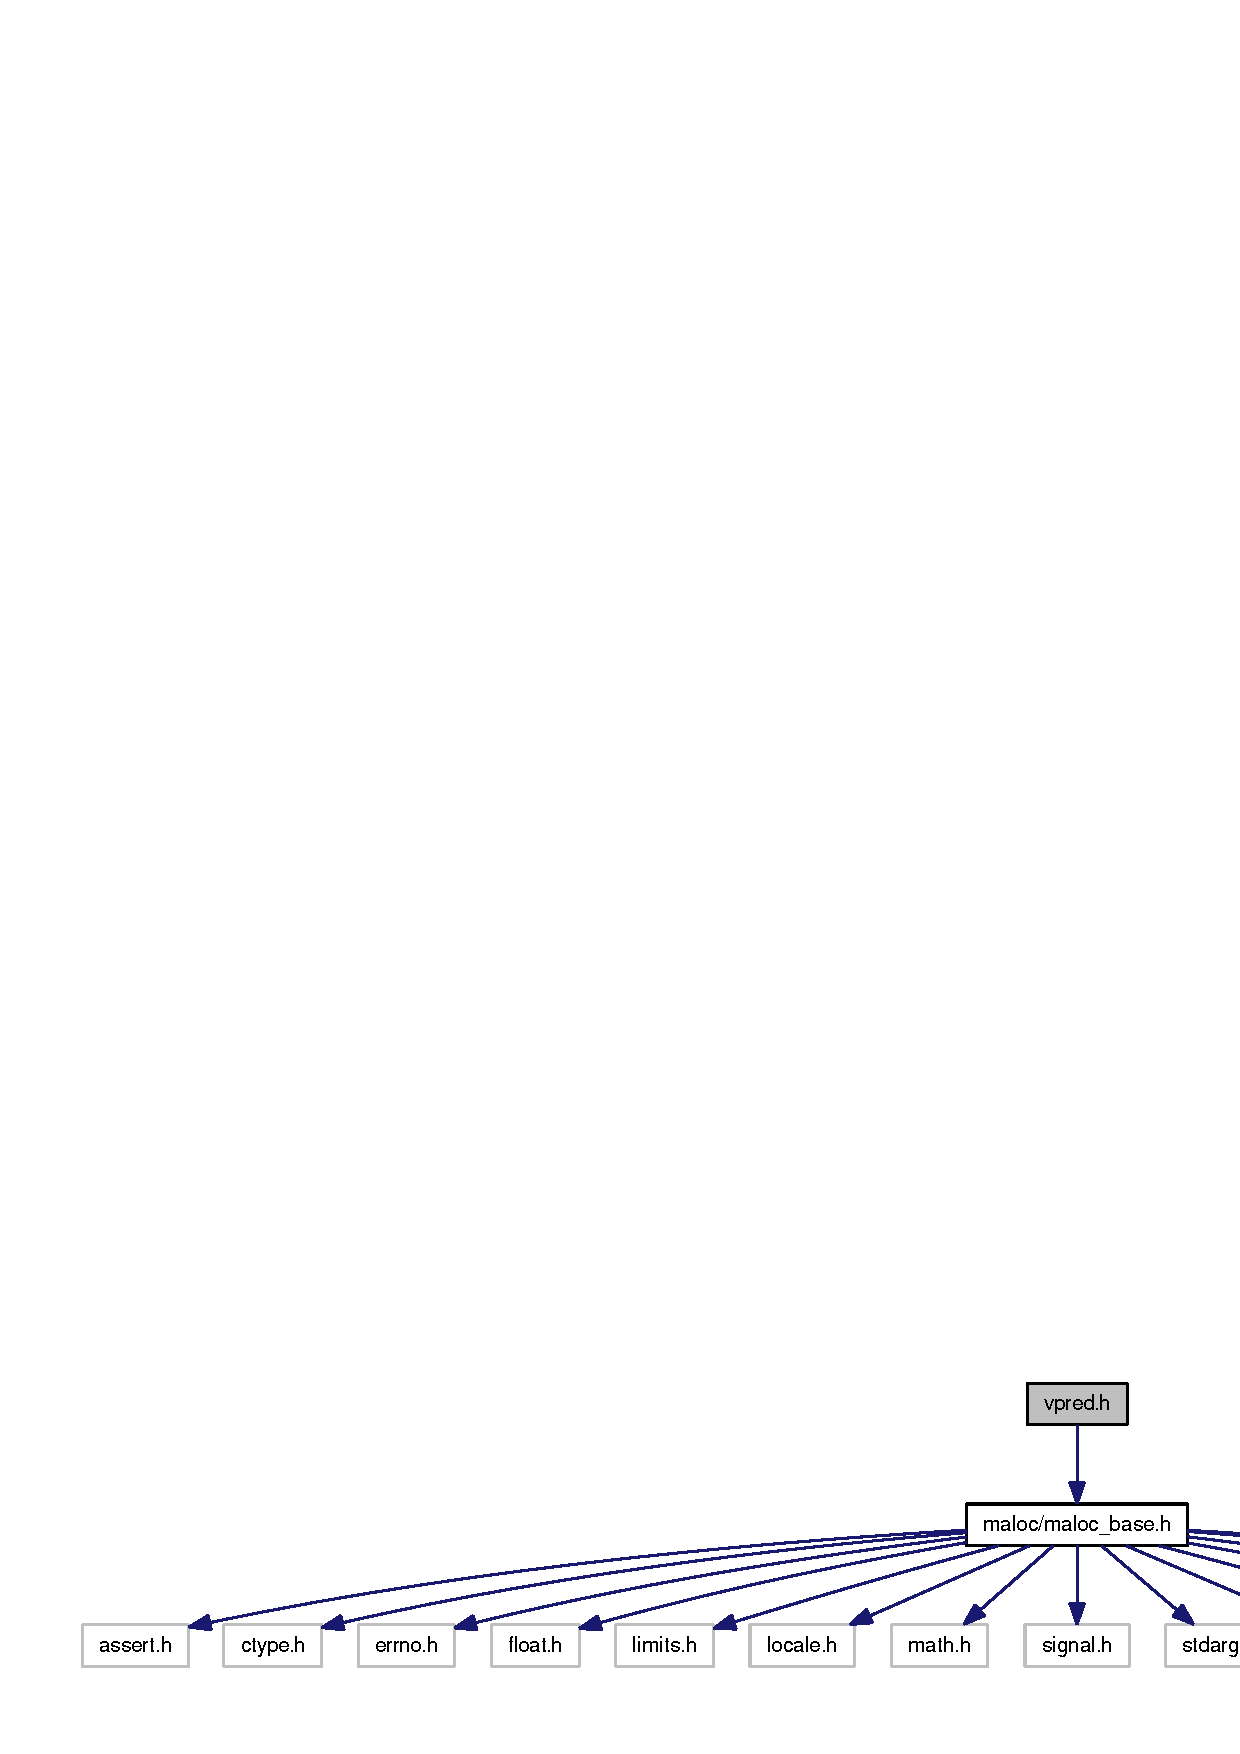
\includegraphics[width=400pt]{a00049}
\end{center}
\end{figure}
This graph shows which files directly or indirectly include this file:
\nopagebreak
\begin{figure}[H]
\begin{center}
\leavevmode
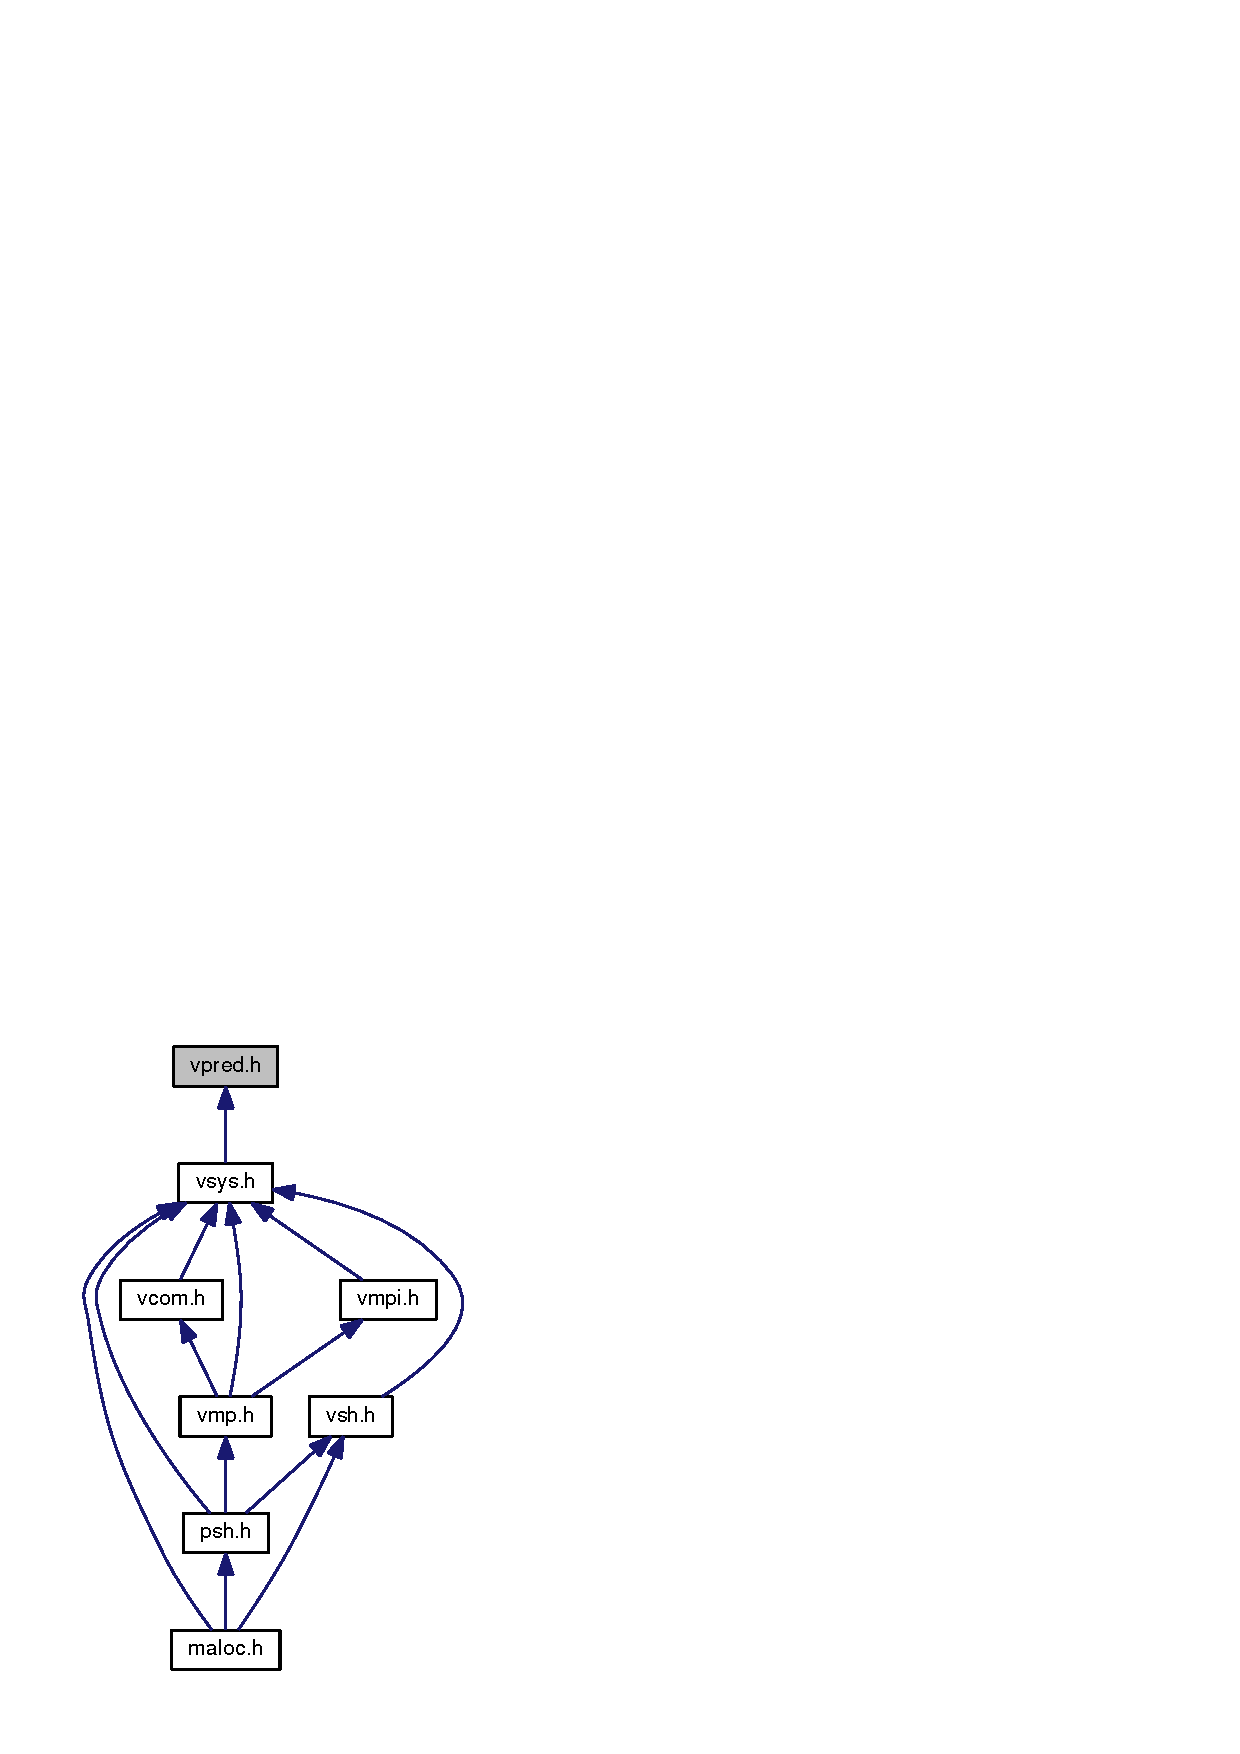
\includegraphics[width=224pt]{a00050}
\end{center}
\end{figure}
\subsection*{Defines}
\begin{DoxyCompactItemize}
\item 
\#define {\bf INEXACT}
\begin{DoxyCompactList}\small\item\em Parameters and constants \char`\"{}INEXACT\char`\"{}. \item\end{DoxyCompactList}\item 
\#define {\bf REAL}~double
\begin{DoxyCompactList}\small\item\em float or double \item\end{DoxyCompactList}\item 
\#define {\bf REALPRINT}~doubleprint
\begin{DoxyCompactList}\small\item\em Print the bit representation of a double. \item\end{DoxyCompactList}\item 
\#define {\bf REALRAND}~doublerand
\begin{DoxyCompactList}\small\item\em Generate a double with random 53-\/bit significand and a random exponent in [0, 511]. \item\end{DoxyCompactList}\item 
\#define {\bf NARROWRAND}~narrowdoublerand
\begin{DoxyCompactList}\small\item\em Generate a double with random 53-\/bit significand and a random exponent in [0, 7]. \item\end{DoxyCompactList}\item 
\#define {\bf UNIFORMRAND}~uniformdoublerand
\begin{DoxyCompactList}\small\item\em Generate a double with random 53-\/bit significand. \item\end{DoxyCompactList}\end{DoxyCompactItemize}
\subsection*{Functions}
\begin{DoxyCompactItemize}
\item 
void {\bf Vpred\_\-exactinit} (void)
\begin{DoxyCompactList}\small\item\em Initialize the variables used for exact arithmetic. \item\end{DoxyCompactList}\item 
REAL {\bf Vpred\_\-orient2d} (REAL $\ast$pa, REAL $\ast$pb, REAL $\ast$pc)
\begin{DoxyCompactList}\small\item\em Adaptive exact 2D orientation test. Robust. \item\end{DoxyCompactList}\item 
REAL {\bf Vpred\_\-orient2dfast} (REAL $\ast$pa, REAL $\ast$pb, REAL $\ast$pc)
\begin{DoxyCompactList}\small\item\em Approximate 2D orientation test. Nonrobust. \item\end{DoxyCompactList}\item 
REAL {\bf Vpred\_\-orient2dexact} (REAL $\ast$pa, REAL $\ast$pb, REAL $\ast$pc)
\begin{DoxyCompactList}\small\item\em Exact 2D orientation test. Robust. \item\end{DoxyCompactList}\item 
REAL {\bf Vpred\_\-orient3d} (REAL $\ast$pa, REAL $\ast$pb, REAL $\ast$pc, REAL $\ast$pd)
\begin{DoxyCompactList}\small\item\em Adaptive exact 3D orientation test. Robust. \item\end{DoxyCompactList}\item 
REAL {\bf Vpred\_\-orient3dfast} (REAL $\ast$pa, REAL $\ast$pb, REAL $\ast$pc, REAL $\ast$pd)
\begin{DoxyCompactList}\small\item\em Approximate 3D orientation test. Nonrobust. \item\end{DoxyCompactList}\item 
REAL {\bf Vpred\_\-orient3dexact} (REAL $\ast$pa, REAL $\ast$pb, REAL $\ast$pc, REAL $\ast$pd)
\begin{DoxyCompactList}\small\item\em Exact 3D orientation test. Robust. \item\end{DoxyCompactList}\item 
REAL {\bf Vpred\_\-incircle} (REAL $\ast$pa, REAL $\ast$pb, REAL $\ast$pc, REAL $\ast$pd)
\begin{DoxyCompactList}\small\item\em Adaptive exact 2D incircle test. Robust. \item\end{DoxyCompactList}\item 
REAL {\bf Vpred\_\-incirclefast} (REAL $\ast$pa, REAL $\ast$pb, REAL $\ast$pc, REAL $\ast$pd)
\begin{DoxyCompactList}\small\item\em Approximate 2D incircle test. Nonrobust. \item\end{DoxyCompactList}\item 
REAL {\bf Vpred\_\-incircleexact} (REAL $\ast$pa, REAL $\ast$pb, REAL $\ast$pc, REAL $\ast$pd)
\begin{DoxyCompactList}\small\item\em Exact 2D incircle test. Robust. \item\end{DoxyCompactList}\item 
REAL {\bf Vpred\_\-insphere} (REAL $\ast$pa, REAL $\ast$pb, REAL $\ast$pc, REAL $\ast$pd, REAL $\ast$pe)
\begin{DoxyCompactList}\small\item\em Adaptive exact 3D insphere test. Robust. \item\end{DoxyCompactList}\item 
REAL {\bf Vpred\_\-inspherefast} (REAL $\ast$pa, REAL $\ast$pb, REAL $\ast$pc, REAL $\ast$pd, REAL $\ast$pe)
\begin{DoxyCompactList}\small\item\em Approximate 3D insphere test. Nonrobust. \item\end{DoxyCompactList}\item 
REAL {\bf Vpred\_\-insphereexact} (REAL $\ast$pa, REAL $\ast$pb, REAL $\ast$pc, REAL $\ast$pd, REAL $\ast$pe)
\begin{DoxyCompactList}\small\item\em Exact 3D insphere test. Robust. \item\end{DoxyCompactList}\end{DoxyCompactItemize}


\subsection{Detailed Description}
Header file for the Geometric Predicates. \begin{DoxyVersion}{Version}

\end{DoxyVersion}
\begin{DoxyParagraph}{Id:}
\doxyref{vpred.h}{p.}{a00019},v 1.4 2010/08/12 05:40:37 fetk Exp 
\end{DoxyParagraph}
\begin{DoxyAuthor}{Author}
Michael Holst
\end{DoxyAuthor}
\begin{DoxyAttention}{Attention}
\begin{DoxyVerb}
 *
 * MALOC = < Minimal Abstraction Layer for Object-oriented C >
 * Copyright (C) 1994-- Michael Holst
 *
 * This library is free software; you can redistribute it and/or
 * modify it under the terms of the GNU Lesser General Public
 * License as published by the Free Software Foundation; either
 * version 2.1 of the License, or (at your option) any later version.
 *
 * This library is distributed in the hope that it will be useful,
 * but WITHOUT ANY WARRANTY; without even the implied warranty of
 * MERCHANTABILITY or FITNESS FOR A PARTICULAR PURPOSE. See the GNU
 * Lesser General Public License for more details.
 *
 * You should have received a copy of the GNU Lesser General Public
 * License along with this library; if not, write to the Free Software
 * Foundation, Inc., 59 Temple Place, Suite 330, Boston, MA 02111-1307 USA
 * 
 *  \end{DoxyVerb}
 
\end{DoxyAttention}


\subsection{Define Documentation}
\index{vpred.h@{vpred.h}!INEXACT@{INEXACT}}
\index{INEXACT@{INEXACT}!vpred.h@{vpred.h}}
\subsubsection[{INEXACT}]{\setlength{\rightskip}{0pt plus 5cm}\#define INEXACT}\label{a00019_ad49beae4f708cdfe26352d865ed2eb95}


Parameters and constants \char`\"{}INEXACT\char`\"{}. 

\index{vpred.h@{vpred.h}!NARROWRAND@{NARROWRAND}}
\index{NARROWRAND@{NARROWRAND}!vpred.h@{vpred.h}}
\subsubsection[{NARROWRAND}]{\setlength{\rightskip}{0pt plus 5cm}\#define NARROWRAND~narrowdoublerand}\label{a00019_a573b0e3df6fc0f000607eca1c5569f68}


Generate a double with random 53-\/bit significand and a random exponent in [0, 7]. 

\index{vpred.h@{vpred.h}!REAL@{REAL}}
\index{REAL@{REAL}!vpred.h@{vpred.h}}
\subsubsection[{REAL}]{\setlength{\rightskip}{0pt plus 5cm}\#define REAL~double}\label{a00019_a4b654506f18b8bfd61ad2a29a7e38c25}


float or double 

\index{vpred.h@{vpred.h}!REALPRINT@{REALPRINT}}
\index{REALPRINT@{REALPRINT}!vpred.h@{vpred.h}}
\subsubsection[{REALPRINT}]{\setlength{\rightskip}{0pt plus 5cm}\#define REALPRINT~doubleprint}\label{a00019_a08c32ee2465d67f098ab09bdf0e2eb59}


Print the bit representation of a double. 

\index{vpred.h@{vpred.h}!REALRAND@{REALRAND}}
\index{REALRAND@{REALRAND}!vpred.h@{vpred.h}}
\subsubsection[{REALRAND}]{\setlength{\rightskip}{0pt plus 5cm}\#define REALRAND~doublerand}\label{a00019_a810b77dd5b3d884e1d2641a2e597df22}


Generate a double with random 53-\/bit significand and a random exponent in [0, 511]. 

\index{vpred.h@{vpred.h}!UNIFORMRAND@{UNIFORMRAND}}
\index{UNIFORMRAND@{UNIFORMRAND}!vpred.h@{vpred.h}}
\subsubsection[{UNIFORMRAND}]{\setlength{\rightskip}{0pt plus 5cm}\#define UNIFORMRAND~uniformdoublerand}\label{a00019_a151c130268f15ea9975886f0750f3079}


Generate a double with random 53-\/bit significand. 



\subsection{Function Documentation}
\index{vpred.h@{vpred.h}!Vpred\_\-exactinit@{Vpred\_\-exactinit}}
\index{Vpred\_\-exactinit@{Vpred\_\-exactinit}!vpred.h@{vpred.h}}
\subsubsection[{Vpred\_\-exactinit}]{\setlength{\rightskip}{0pt plus 5cm}void Vpred\_\-exactinit (
\begin{DoxyParamCaption}
\item[{void}]{}
\end{DoxyParamCaption}
)}\label{a00019_a8dbedbfe17e2280b77117d1b9b4cc0b5}


Initialize the variables used for exact arithmetic. 

\begin{DoxyNote}{Note}
`epsilon' is the largest power of two such that 1.0 + epsilon = 1.0 in floating-\/point arithmetic. `epsilon' bounds the relative roundoff error. It is used for floating-\/point error analysis. `splitter' is used to split floating-\/point numbers into two half-\/ length significands for exact multiplication. I imagine that a highly optimizing compiler might be too smart for its own good, and somehow cause this routine to fail, if it pretends that floating-\/point arithmetic is too much like real arithmetic. Don't change this routine unless you fully understand it. 
\end{DoxyNote}
\index{vpred.h@{vpred.h}!Vpred\_\-incircle@{Vpred\_\-incircle}}
\index{Vpred\_\-incircle@{Vpred\_\-incircle}!vpred.h@{vpred.h}}
\subsubsection[{Vpred\_\-incircle}]{\setlength{\rightskip}{0pt plus 5cm}REAL Vpred\_\-incircle (
\begin{DoxyParamCaption}
\item[{REAL $\ast$}]{ pa, }
\item[{REAL $\ast$}]{ pb, }
\item[{REAL $\ast$}]{ pc, }
\item[{REAL $\ast$}]{ pd}
\end{DoxyParamCaption}
)}\label{a00019_add3df6a8e6fa33d79b0af9054a675241}


Adaptive exact 2D incircle test. Robust. 

\begin{DoxyReturn}{Returns}
a positive value if the point pd lies inside the circle passing through pa, pb, and pc; a negative value if it lies outside; and zero if the four points are cocircular. The points pa, pb, and pc must be in counterclockwise order, or the sign of the result will be reversed. 
\end{DoxyReturn}

\begin{DoxyParams}{Parameters}
\item[{\em pa}]Pointer to a real parameter \item[{\em pb}]Pointer to a real parameter \item[{\em pc}]Pointer to a real parameter \item[{\em pd}]Pointer to a real parameter \end{DoxyParams}
\index{vpred.h@{vpred.h}!Vpred\_\-incircleexact@{Vpred\_\-incircleexact}}
\index{Vpred\_\-incircleexact@{Vpred\_\-incircleexact}!vpred.h@{vpred.h}}
\subsubsection[{Vpred\_\-incircleexact}]{\setlength{\rightskip}{0pt plus 5cm}REAL Vpred\_\-incircleexact (
\begin{DoxyParamCaption}
\item[{REAL $\ast$}]{ pa, }
\item[{REAL $\ast$}]{ pb, }
\item[{REAL $\ast$}]{ pc, }
\item[{REAL $\ast$}]{ pd}
\end{DoxyParamCaption}
)}\label{a00019_aa4e7d7af15ac70194aad8a5d7fdbe0fb}


Exact 2D incircle test. Robust. 

\begin{DoxyReturn}{Returns}
a positive value if the point pd lies inside the circle passing through pa, pb, and pc; a negative value if it lies outside; and zero if the four points are cocircular. The points pa, pb, and pc must be in counterclockwise order, or the sign of the result will be reversed. 
\end{DoxyReturn}

\begin{DoxyParams}{Parameters}
\item[{\em pa}]Pointer to a real parameter \item[{\em pb}]Pointer to a real parameter \item[{\em pc}]Pointer to a real parameter \item[{\em pd}]Pointer to a real parameter \end{DoxyParams}
\index{vpred.h@{vpred.h}!Vpred\_\-incirclefast@{Vpred\_\-incirclefast}}
\index{Vpred\_\-incirclefast@{Vpred\_\-incirclefast}!vpred.h@{vpred.h}}
\subsubsection[{Vpred\_\-incirclefast}]{\setlength{\rightskip}{0pt plus 5cm}REAL Vpred\_\-incirclefast (
\begin{DoxyParamCaption}
\item[{REAL $\ast$}]{ pa, }
\item[{REAL $\ast$}]{ pb, }
\item[{REAL $\ast$}]{ pc, }
\item[{REAL $\ast$}]{ pd}
\end{DoxyParamCaption}
)}\label{a00019_adda50e6f7416902e79bf391adc0f191d}


Approximate 2D incircle test. Nonrobust. 

\begin{DoxyReturn}{Returns}
a positive value if the point pd lies inside the circle passing through pa, pb, and pc; a negative value if it lies outside; and zero if the four points are cocircular. The points pa, pb, and pc must be in counterclockwise order, or the sign of the result will be reversed. 
\end{DoxyReturn}

\begin{DoxyParams}{Parameters}
\item[{\em pa}]Pointer to a real parameter \item[{\em pb}]Pointer to a real parameter \item[{\em pc}]Pointer to a real parameter \item[{\em pd}]Pointer to a real parameter \end{DoxyParams}
\index{vpred.h@{vpred.h}!Vpred\_\-insphere@{Vpred\_\-insphere}}
\index{Vpred\_\-insphere@{Vpred\_\-insphere}!vpred.h@{vpred.h}}
\subsubsection[{Vpred\_\-insphere}]{\setlength{\rightskip}{0pt plus 5cm}REAL Vpred\_\-insphere (
\begin{DoxyParamCaption}
\item[{REAL $\ast$}]{ pa, }
\item[{REAL $\ast$}]{ pb, }
\item[{REAL $\ast$}]{ pc, }
\item[{REAL $\ast$}]{ pd, }
\item[{REAL $\ast$}]{ pe}
\end{DoxyParamCaption}
)}\label{a00019_ac4811e37c08e6aa1069066be5d77c9f1}


Adaptive exact 3D insphere test. Robust. 

\begin{DoxyReturn}{Returns}
a positive value if the point pe lies inside the sphere passing through pa, pb, pc, and pd; a negative value if it lies outside; and zero if the five points are cospherical. The points pa, pb, pc, and pd must be ordered so that they have a positive orientation (as defined by orient3d()), or the sign of the result will be reversed. 
\end{DoxyReturn}

\begin{DoxyParams}{Parameters}
\item[{\em pa}]Pointer to a real parameter \item[{\em pb}]Pointer to a real parameter \item[{\em pc}]Pointer to a real parameter \item[{\em pd}]Pointer to a real parameter \item[{\em pe}]Pointer to a real parameter \end{DoxyParams}
\index{vpred.h@{vpred.h}!Vpred\_\-insphereexact@{Vpred\_\-insphereexact}}
\index{Vpred\_\-insphereexact@{Vpred\_\-insphereexact}!vpred.h@{vpred.h}}
\subsubsection[{Vpred\_\-insphereexact}]{\setlength{\rightskip}{0pt plus 5cm}REAL Vpred\_\-insphereexact (
\begin{DoxyParamCaption}
\item[{REAL $\ast$}]{ pa, }
\item[{REAL $\ast$}]{ pb, }
\item[{REAL $\ast$}]{ pc, }
\item[{REAL $\ast$}]{ pd, }
\item[{REAL $\ast$}]{ pe}
\end{DoxyParamCaption}
)}\label{a00019_a7a354011003573a544c661bc8c9629bb}


Exact 3D insphere test. Robust. 

\begin{DoxyReturn}{Returns}
a positive value if the point pe lies inside the sphere passing through pa, pb, pc, and pd; a negative value if it lies outside; and zero if the five points are cospherical. The points pa, pb, pc, and pd must be ordered so that they have a positive orientation (as defined by orient3d()), or the sign of the result will be reversed. 
\end{DoxyReturn}

\begin{DoxyParams}{Parameters}
\item[{\em pa}]Pointer to a real parameter \item[{\em pb}]Pointer to a real parameter \item[{\em pc}]Pointer to a real parameter \item[{\em pd}]Pointer to a real parameter \item[{\em pe}]Pointer to a real parameter \end{DoxyParams}
\index{vpred.h@{vpred.h}!Vpred\_\-inspherefast@{Vpred\_\-inspherefast}}
\index{Vpred\_\-inspherefast@{Vpred\_\-inspherefast}!vpred.h@{vpred.h}}
\subsubsection[{Vpred\_\-inspherefast}]{\setlength{\rightskip}{0pt plus 5cm}REAL Vpred\_\-inspherefast (
\begin{DoxyParamCaption}
\item[{REAL $\ast$}]{ pa, }
\item[{REAL $\ast$}]{ pb, }
\item[{REAL $\ast$}]{ pc, }
\item[{REAL $\ast$}]{ pd, }
\item[{REAL $\ast$}]{ pe}
\end{DoxyParamCaption}
)}\label{a00019_a584298eaa7bbdc87d619555403c7d061}


Approximate 3D insphere test. Nonrobust. 

\begin{DoxyReturn}{Returns}
a positive value if the point pe lies inside the sphere passing through pa, pb, pc, and pd; a negative value if it lies outside; and zero if the five points are cospherical. The points pa, pb, pc, and pd must be ordered so that they have a positive orientation (as defined by orient3d()), or the sign of the result will be reversed. 
\end{DoxyReturn}

\begin{DoxyParams}{Parameters}
\item[{\em pa}]Pointer to a real parameter \item[{\em pb}]Pointer to a real parameter \item[{\em pc}]Pointer to a real parameter \item[{\em pd}]Pointer to a real parameter \item[{\em pe}]Pointer to a real parameter \end{DoxyParams}
\index{vpred.h@{vpred.h}!Vpred\_\-orient2d@{Vpred\_\-orient2d}}
\index{Vpred\_\-orient2d@{Vpred\_\-orient2d}!vpred.h@{vpred.h}}
\subsubsection[{Vpred\_\-orient2d}]{\setlength{\rightskip}{0pt plus 5cm}REAL Vpred\_\-orient2d (
\begin{DoxyParamCaption}
\item[{REAL $\ast$}]{ pa, }
\item[{REAL $\ast$}]{ pb, }
\item[{REAL $\ast$}]{ pc}
\end{DoxyParamCaption}
)}\label{a00019_a0bc8c96f96cc9ad2a6fa911e6f426f75}


Adaptive exact 2D orientation test. Robust. 

\begin{DoxyReturn}{Returns}
a positive value if the points pa, pb, and pc occur in counterclockwise order; a negative value if they occur in clockwise order; and zero if they are collinear. The result is also a rough approximation of twice the signed area of the triangle defined by the three points. 
\end{DoxyReturn}

\begin{DoxyParams}{Parameters}
\item[{\em pa}]Pointer to a real parameter \item[{\em pb}]Pointer to a real parameter \item[{\em pc}]Pointer to a real parameter \end{DoxyParams}
\index{vpred.h@{vpred.h}!Vpred\_\-orient2dexact@{Vpred\_\-orient2dexact}}
\index{Vpred\_\-orient2dexact@{Vpred\_\-orient2dexact}!vpred.h@{vpred.h}}
\subsubsection[{Vpred\_\-orient2dexact}]{\setlength{\rightskip}{0pt plus 5cm}REAL Vpred\_\-orient2dexact (
\begin{DoxyParamCaption}
\item[{REAL $\ast$}]{ pa, }
\item[{REAL $\ast$}]{ pb, }
\item[{REAL $\ast$}]{ pc}
\end{DoxyParamCaption}
)}\label{a00019_acc0ab2f55dd3e1132e1bb34bb64d14e1}


Exact 2D orientation test. Robust. 

\begin{DoxyReturn}{Returns}
a positive value if the points pa, pb, and pc occur in counterclockwise order; a negative value if they occur in clockwise order; and zero if they are collinear. The result is also a rough approximation of twice the signed area of the triangle defined by the three points. 
\end{DoxyReturn}

\begin{DoxyParams}{Parameters}
\item[{\em pa}]Pointer to a real parameter \item[{\em pb}]Pointer to a real parameter \item[{\em pc}]Pointer to a real parameter \end{DoxyParams}
\index{vpred.h@{vpred.h}!Vpred\_\-orient2dfast@{Vpred\_\-orient2dfast}}
\index{Vpred\_\-orient2dfast@{Vpred\_\-orient2dfast}!vpred.h@{vpred.h}}
\subsubsection[{Vpred\_\-orient2dfast}]{\setlength{\rightskip}{0pt plus 5cm}REAL Vpred\_\-orient2dfast (
\begin{DoxyParamCaption}
\item[{REAL $\ast$}]{ pa, }
\item[{REAL $\ast$}]{ pb, }
\item[{REAL $\ast$}]{ pc}
\end{DoxyParamCaption}
)}\label{a00019_ac486c720889544acae5950a94be4876e}


Approximate 2D orientation test. Nonrobust. 

\begin{DoxyReturn}{Returns}
a positive value if the points pa, pb, and pc occur in counterclockwise order; a negative value if they occur in clockwise order; and zero if they are collinear. The result is also a rough approximation of twice the signed area of the triangle defined by the three points. 
\end{DoxyReturn}

\begin{DoxyParams}{Parameters}
\item[{\em pa}]Pointer to a real parameter \item[{\em pb}]Pointer to a real parameter \item[{\em pc}]Pointer to a real parameter \end{DoxyParams}
\index{vpred.h@{vpred.h}!Vpred\_\-orient3d@{Vpred\_\-orient3d}}
\index{Vpred\_\-orient3d@{Vpred\_\-orient3d}!vpred.h@{vpred.h}}
\subsubsection[{Vpred\_\-orient3d}]{\setlength{\rightskip}{0pt plus 5cm}REAL Vpred\_\-orient3d (
\begin{DoxyParamCaption}
\item[{REAL $\ast$}]{ pa, }
\item[{REAL $\ast$}]{ pb, }
\item[{REAL $\ast$}]{ pc, }
\item[{REAL $\ast$}]{ pd}
\end{DoxyParamCaption}
)}\label{a00019_a69ab7e33e86529fdf82c56a4d0086af6}


Adaptive exact 3D orientation test. Robust. 

\begin{DoxyReturn}{Returns}
a positive value if the point pd lies below the plane passing through pa, pb, and pc; \char`\"{}below\char`\"{} is defined so that pa, pb, and pc appear in counterclockwise order when viewed from above the plane. Returns a negative value if pd lies above the plane. Returns zero if the points are coplanar. The result is also a rough approximation of six times the signed volume of the tetrahedron defined by the four points. 
\end{DoxyReturn}

\begin{DoxyParams}{Parameters}
\item[{\em pa}]Pointer to a real parameter \item[{\em pb}]Pointer to a real parameter \item[{\em pc}]Pointer to a real parameter \item[{\em pd}]Pointer to a real parameter \end{DoxyParams}
\index{vpred.h@{vpred.h}!Vpred\_\-orient3dexact@{Vpred\_\-orient3dexact}}
\index{Vpred\_\-orient3dexact@{Vpred\_\-orient3dexact}!vpred.h@{vpred.h}}
\subsubsection[{Vpred\_\-orient3dexact}]{\setlength{\rightskip}{0pt plus 5cm}REAL Vpred\_\-orient3dexact (
\begin{DoxyParamCaption}
\item[{REAL $\ast$}]{ pa, }
\item[{REAL $\ast$}]{ pb, }
\item[{REAL $\ast$}]{ pc, }
\item[{REAL $\ast$}]{ pd}
\end{DoxyParamCaption}
)}\label{a00019_a4fd309b85b6eba9b2b949e8cd408d077}


Exact 3D orientation test. Robust. 

\begin{DoxyReturn}{Returns}
a positive value if the point pd lies below the plane passing through pa, pb, and pc; \char`\"{}below\char`\"{} is defined so that pa, pb, and pc appear in counterclockwise order when viewed from above the plane. Returns a negative value if pd lies above the plane. Returns zero if the points are coplanar. The result is also a rough approximation of six times the signed volume of the tetrahedron defined by the four points. 
\end{DoxyReturn}

\begin{DoxyParams}{Parameters}
\item[{\em pa}]Pointer to a real parameter \item[{\em pb}]Pointer to a real parameter \item[{\em pc}]Pointer to a real parameter \item[{\em pd}]Pointer to a real parameter \end{DoxyParams}
\index{vpred.h@{vpred.h}!Vpred\_\-orient3dfast@{Vpred\_\-orient3dfast}}
\index{Vpred\_\-orient3dfast@{Vpred\_\-orient3dfast}!vpred.h@{vpred.h}}
\subsubsection[{Vpred\_\-orient3dfast}]{\setlength{\rightskip}{0pt plus 5cm}REAL Vpred\_\-orient3dfast (
\begin{DoxyParamCaption}
\item[{REAL $\ast$}]{ pa, }
\item[{REAL $\ast$}]{ pb, }
\item[{REAL $\ast$}]{ pc, }
\item[{REAL $\ast$}]{ pd}
\end{DoxyParamCaption}
)}\label{a00019_a20697c6349d030052c71e083c23348cb}


Approximate 3D orientation test. Nonrobust. 

\begin{DoxyReturn}{Returns}
a positive value if the point pd lies below the plane passing through pa, pb, and pc; \char`\"{}below\char`\"{} is defined so that pa, pb, and pc appear in counterclockwise order when viewed from above the plane. Returns a negative value if pd lies above the plane. Returns zero if the points are coplanar. The result is also a rough approximation of six times the signed volume of the tetrahedron defined by the four points. 
\end{DoxyReturn}

\begin{DoxyParams}{Parameters}
\item[{\em pa}]Pointer to a real parameter \item[{\em pb}]Pointer to a real parameter \item[{\em pc}]Pointer to a real parameter \item[{\em pd}]Pointer to a real parameter \end{DoxyParams}

\section{vset.\+h File Reference}
\label{a00020}\index{vset.\+h@{vset.\+h}}


Class Vset\+: a dynamic set object.  


{\ttfamily \#include $<$maloc/maloc\+\_\+base.\+h$>$}\\*
{\ttfamily \#include $<$maloc/vnm.\+h$>$}\\*
{\ttfamily \#include $<$maloc/vmem.\+h$>$}\\*
Include dependency graph for vset.\+h\+:\nopagebreak
\begin{figure}[H]
\begin{center}
\leavevmode
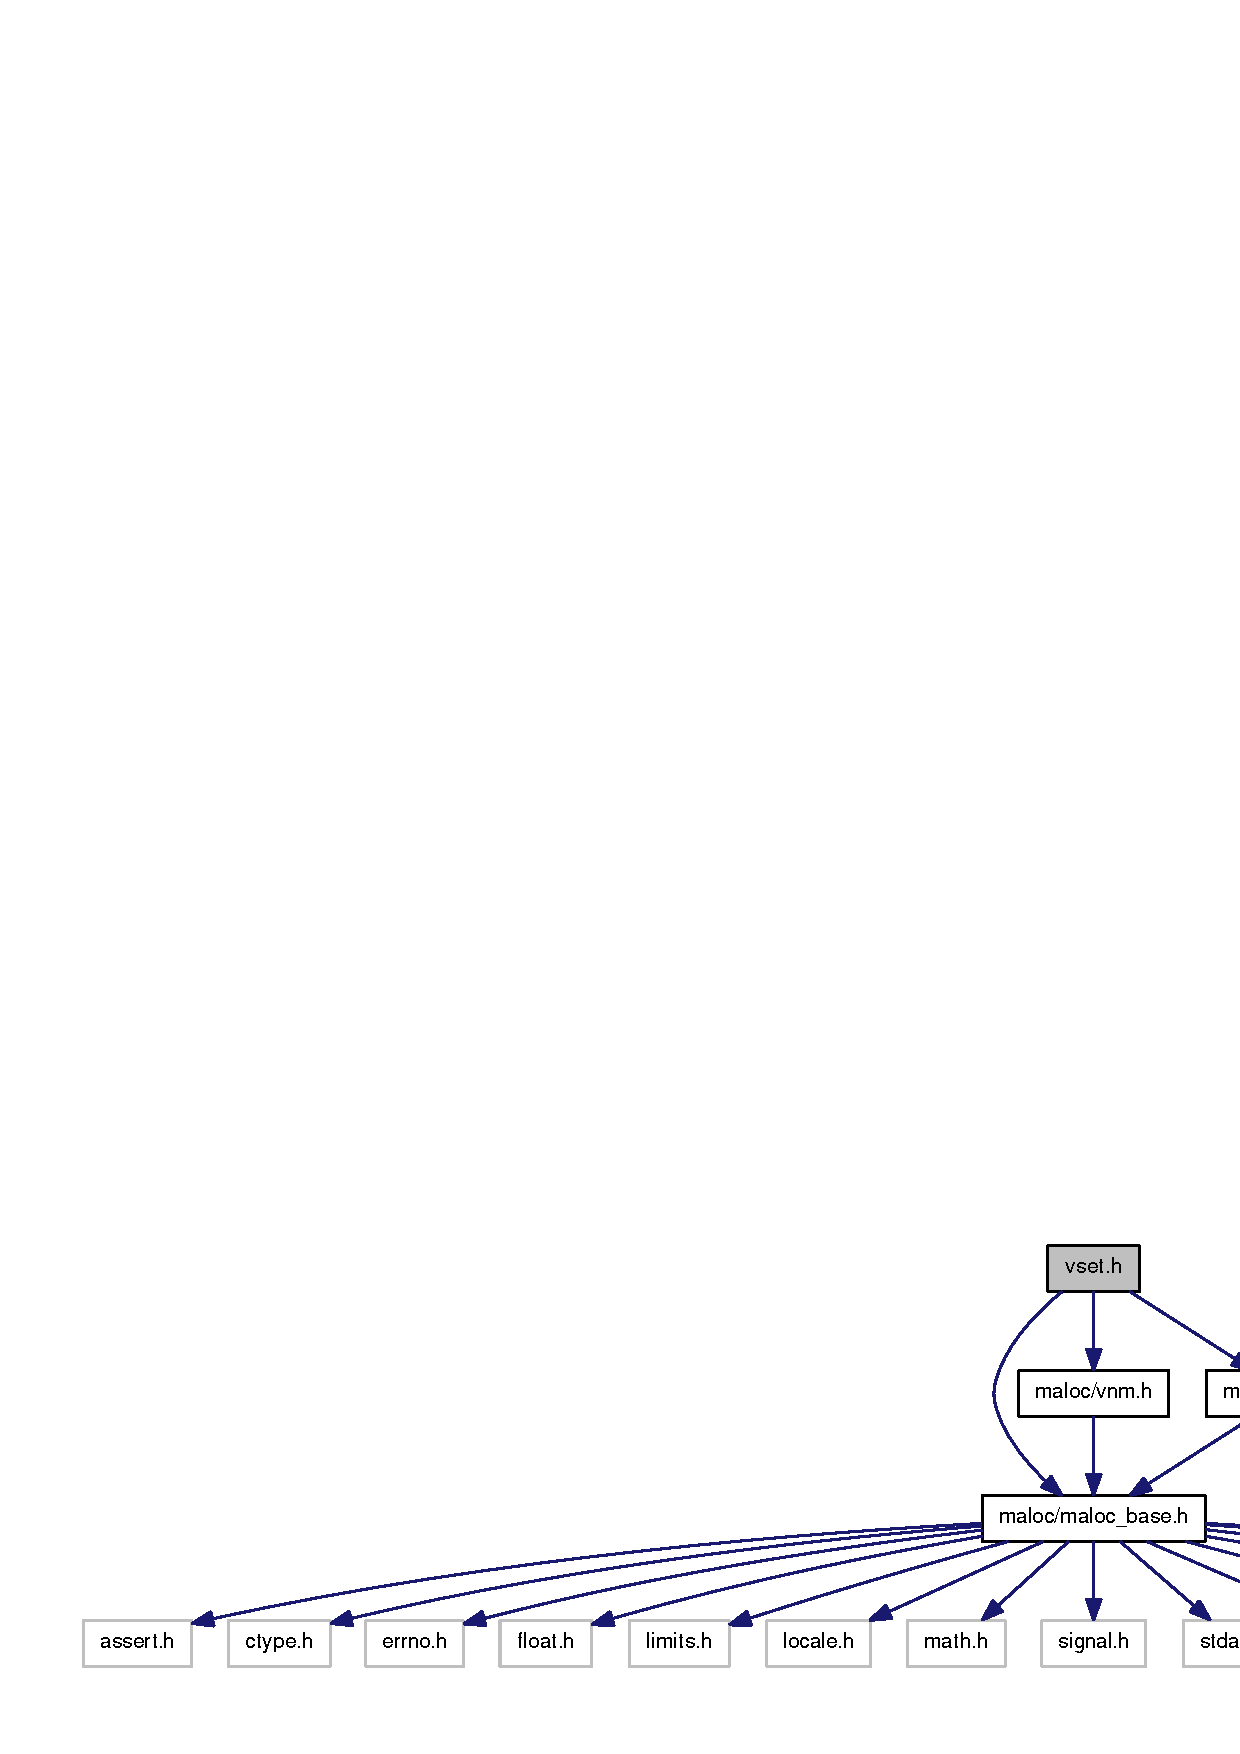
\includegraphics[width=350pt]{a00051}
\end{center}
\end{figure}
This graph shows which files directly or indirectly include this file\+:\nopagebreak
\begin{figure}[H]
\begin{center}
\leavevmode
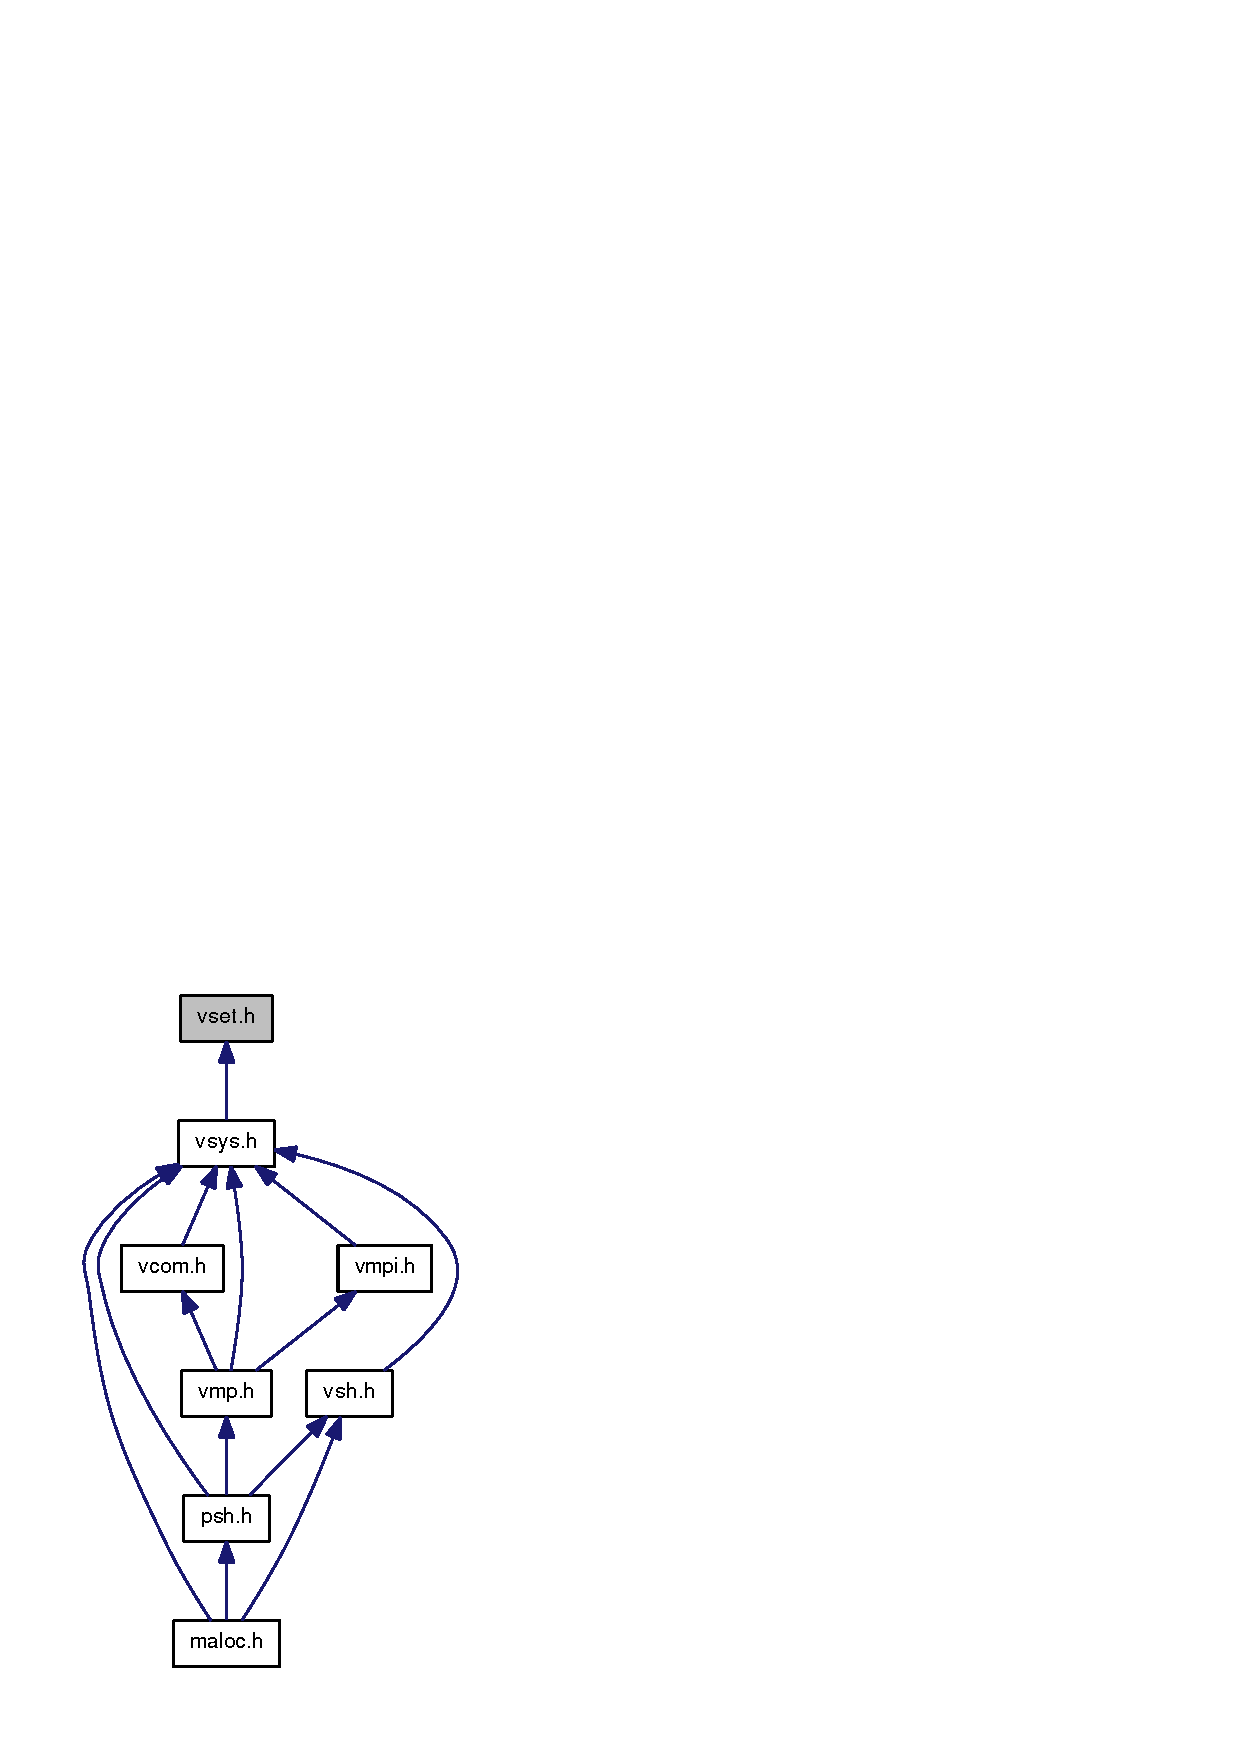
\includegraphics[width=224pt]{a00052}
\end{center}
\end{figure}
\subsection*{Classes}
\begin{DoxyCompactItemize}
\item 
struct {\bf s\+Vset}
\begin{DoxyCompactList}\small\item\em Contains public data members for Vset class. \end{DoxyCompactList}\end{DoxyCompactItemize}
\subsection*{Typedefs}
\begin{DoxyCompactItemize}
\item 
typedef struct {\bf s\+Vset} {\bf Vset}
\begin{DoxyCompactList}\small\item\em Declaration of the Vset class as the Vset structure. \end{DoxyCompactList}\end{DoxyCompactItemize}
\subsection*{Functions}
\begin{DoxyCompactItemize}
\item 
int {\bf Vset\+\_\+num} ({\bf Vset} $\ast$thee)
\begin{DoxyCompactList}\small\item\em Return the number of things currently in the list. \end{DoxyCompactList}\item 
char $\ast$ {\bf Vset\+\_\+access} ({\bf Vset} $\ast$thee, int i)
\begin{DoxyCompactList}\small\item\em Access an object in an arbitrary place in the list. \end{DoxyCompactList}\item 
char $\ast$ {\bf Vset\+\_\+create} ({\bf Vset} $\ast$thee)
\begin{DoxyCompactList}\small\item\em Create an object on the end of the list. \end{DoxyCompactList}\item 
char $\ast$ {\bf Vset\+\_\+first} ({\bf Vset} $\ast$thee)
\begin{DoxyCompactList}\small\item\em Return the first object in the set. \end{DoxyCompactList}\item 
char $\ast$ {\bf Vset\+\_\+last} ({\bf Vset} $\ast$thee)
\begin{DoxyCompactList}\small\item\em Return the last object in the set. \end{DoxyCompactList}\item 
char $\ast$ {\bf Vset\+\_\+next} ({\bf Vset} $\ast$thee)
\begin{DoxyCompactList}\small\item\em Return the next object in the set. \end{DoxyCompactList}\item 
char $\ast$ {\bf Vset\+\_\+prev} ({\bf Vset} $\ast$thee)
\begin{DoxyCompactList}\small\item\em Return the prev object in the set. \end{DoxyCompactList}\item 
char $\ast$ {\bf Vset\+\_\+peek\+First} ({\bf Vset} $\ast$thee)
\begin{DoxyCompactList}\small\item\em Return the first object in the set. \end{DoxyCompactList}\item 
char $\ast$ {\bf Vset\+\_\+peek\+Last} ({\bf Vset} $\ast$thee)
\begin{DoxyCompactList}\small\item\em Return the last object in the set. \end{DoxyCompactList}\item 
void {\bf Vset\+\_\+destroy} ({\bf Vset} $\ast$thee)
\begin{DoxyCompactList}\small\item\em Delete an object from the end of the list. \end{DoxyCompactList}\item 
{\bf Vset} $\ast$ {\bf Vset\+\_\+ctor} ({\bf Vmem} $\ast$vmem, const char $\ast$tname, int tsize, int tmax\+Num, int io\+Key)
\begin{DoxyCompactList}\small\item\em Construct the set object. \end{DoxyCompactList}\item 
void {\bf Vset\+\_\+dtor} ({\bf Vset} $\ast$$\ast$thee)
\begin{DoxyCompactList}\small\item\em Destroy the set object. \end{DoxyCompactList}\item 
char $\ast$ {\bf Vset\+\_\+create\+Last} ({\bf Vset} $\ast$thee)
\begin{DoxyCompactList}\small\item\em Create an object on the end of the list. \end{DoxyCompactList}\item 
void {\bf Vset\+\_\+destroy\+Last} ({\bf Vset} $\ast$thee)
\begin{DoxyCompactList}\small\item\em Free up the object currently on the end of the list. \end{DoxyCompactList}\item 
void {\bf Vset\+\_\+init\+Data} ({\bf Vset} $\ast$thee)
\begin{DoxyCompactList}\small\item\em Initialize the Vset data (thee). \end{DoxyCompactList}\item 
void {\bf Vset\+\_\+reset} ({\bf Vset} $\ast$thee)
\begin{DoxyCompactList}\small\item\em Release all Ram controlled by this (thee) and re-\/initialize. \end{DoxyCompactList}\item 
void {\bf Vset\+\_\+check} ({\bf Vset} $\ast$thee, int $\ast$tnum, int $\ast$tsize, int $\ast$t\+Vec\+Use, int $\ast$t\+Vec\+Mal, int $\ast$t\+Vec\+Ohd)
\begin{DoxyCompactList}\small\item\em Get and return the R\+A\+M Control Block (thee) information. \end{DoxyCompactList}\item 
void {\bf Vset\+\_\+mem\+Chk} ({\bf Vset} $\ast$thee)
\begin{DoxyCompactList}\small\item\em Print the exact current malloc usage. \end{DoxyCompactList}\end{DoxyCompactItemize}


\subsection{Detailed Description}
Class Vset\+: a dynamic set object. 

\begin{DoxyAuthor}{Author}
Michael Holst 
\end{DoxyAuthor}
\begin{DoxyNote}{Note}
None 
\end{DoxyNote}
\begin{DoxyVersion}{Version}

\end{DoxyVersion}
\begin{DoxyParagraph}{Id}
\doxyref{vset.\+h}{p.}{a00020},v 1.\+20 2010/08/12 05\+:40\+:37 fetk Exp 
\end{DoxyParagraph}


\begin{DoxyAttention}{Attention}
\begin{DoxyVerb}*
* MALOC = < Minimal Abstraction Layer for Object-oriented C >
* Copyright (C) 1994-- Michael Holst
*
* This library is free software; you can redistribute it and/or
* modify it under the terms of the GNU Lesser General Public
* License as published by the Free Software Foundation; either
* version 2.1 of the License, or (at your option) any later version.
*
* This library is distributed in the hope that it will be useful,
* but WITHOUT ANY WARRANTY; without even the implied warranty of
* MERCHANTABILITY or FITNESS FOR A PARTICULAR PURPOSE. See the GNU
* Lesser General Public License for more details.
*
* You should have received a copy of the GNU Lesser General Public
* License along with this library; if not, write to the Free Software
* Foundation, Inc., 59 Temple Place, Suite 330, Boston, MA 02111-1307 USA
* 
*  \end{DoxyVerb}
 
\end{DoxyAttention}

\section{vsh.h File Reference}
\label{a00021}\index{vsh.h@{vsh.h}}


Header file for vsh, a bourne-\/compatible shell.  


{\ttfamily \#include $<$maloc/maloc\_\-base.h$>$}\par
{\ttfamily \#include $<$maloc/vsys.h$>$}\par
Include dependency graph for vsh.h:
\nopagebreak
\begin{figure}[H]
\begin{center}
\leavevmode
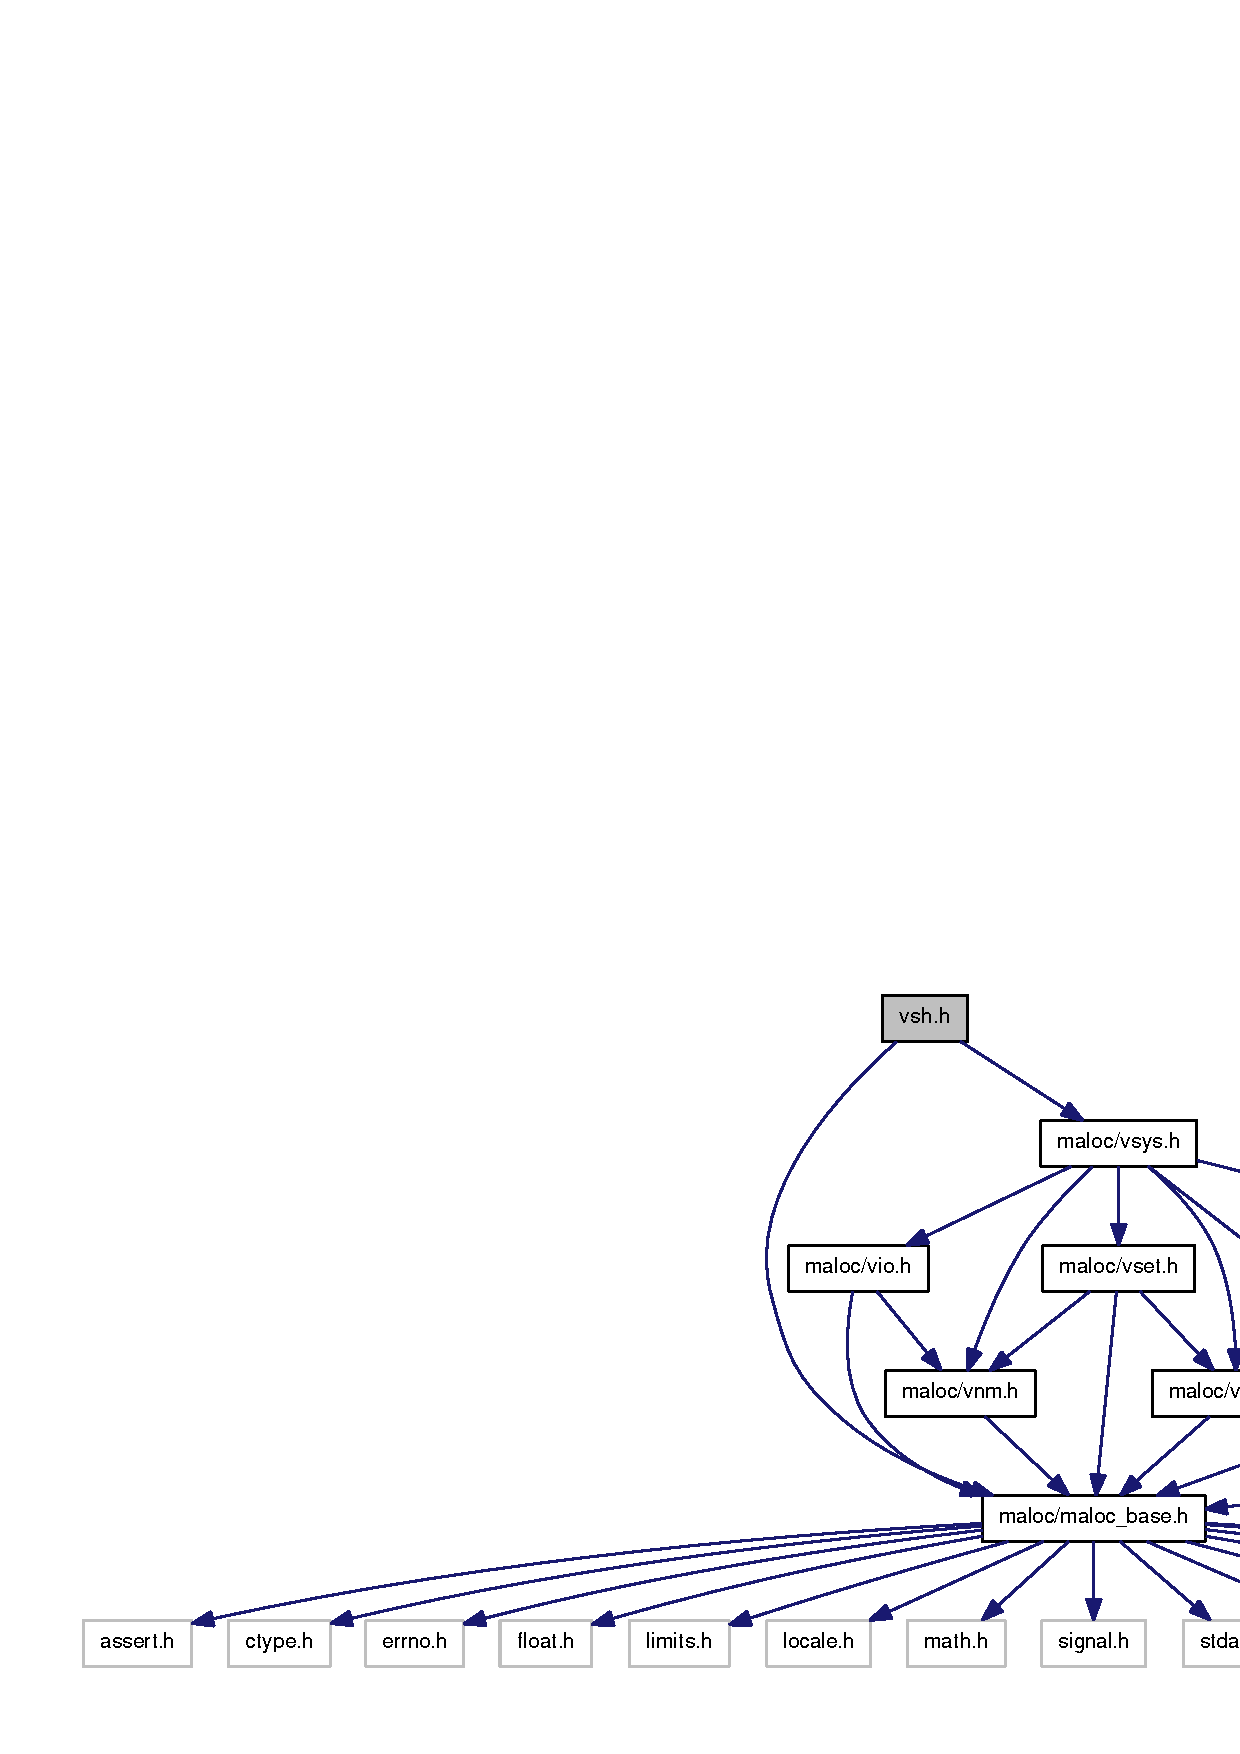
\includegraphics[width=400pt]{a00053}
\end{center}
\end{figure}
This graph shows which files directly or indirectly include this file:
\nopagebreak
\begin{figure}[H]
\begin{center}
\leavevmode
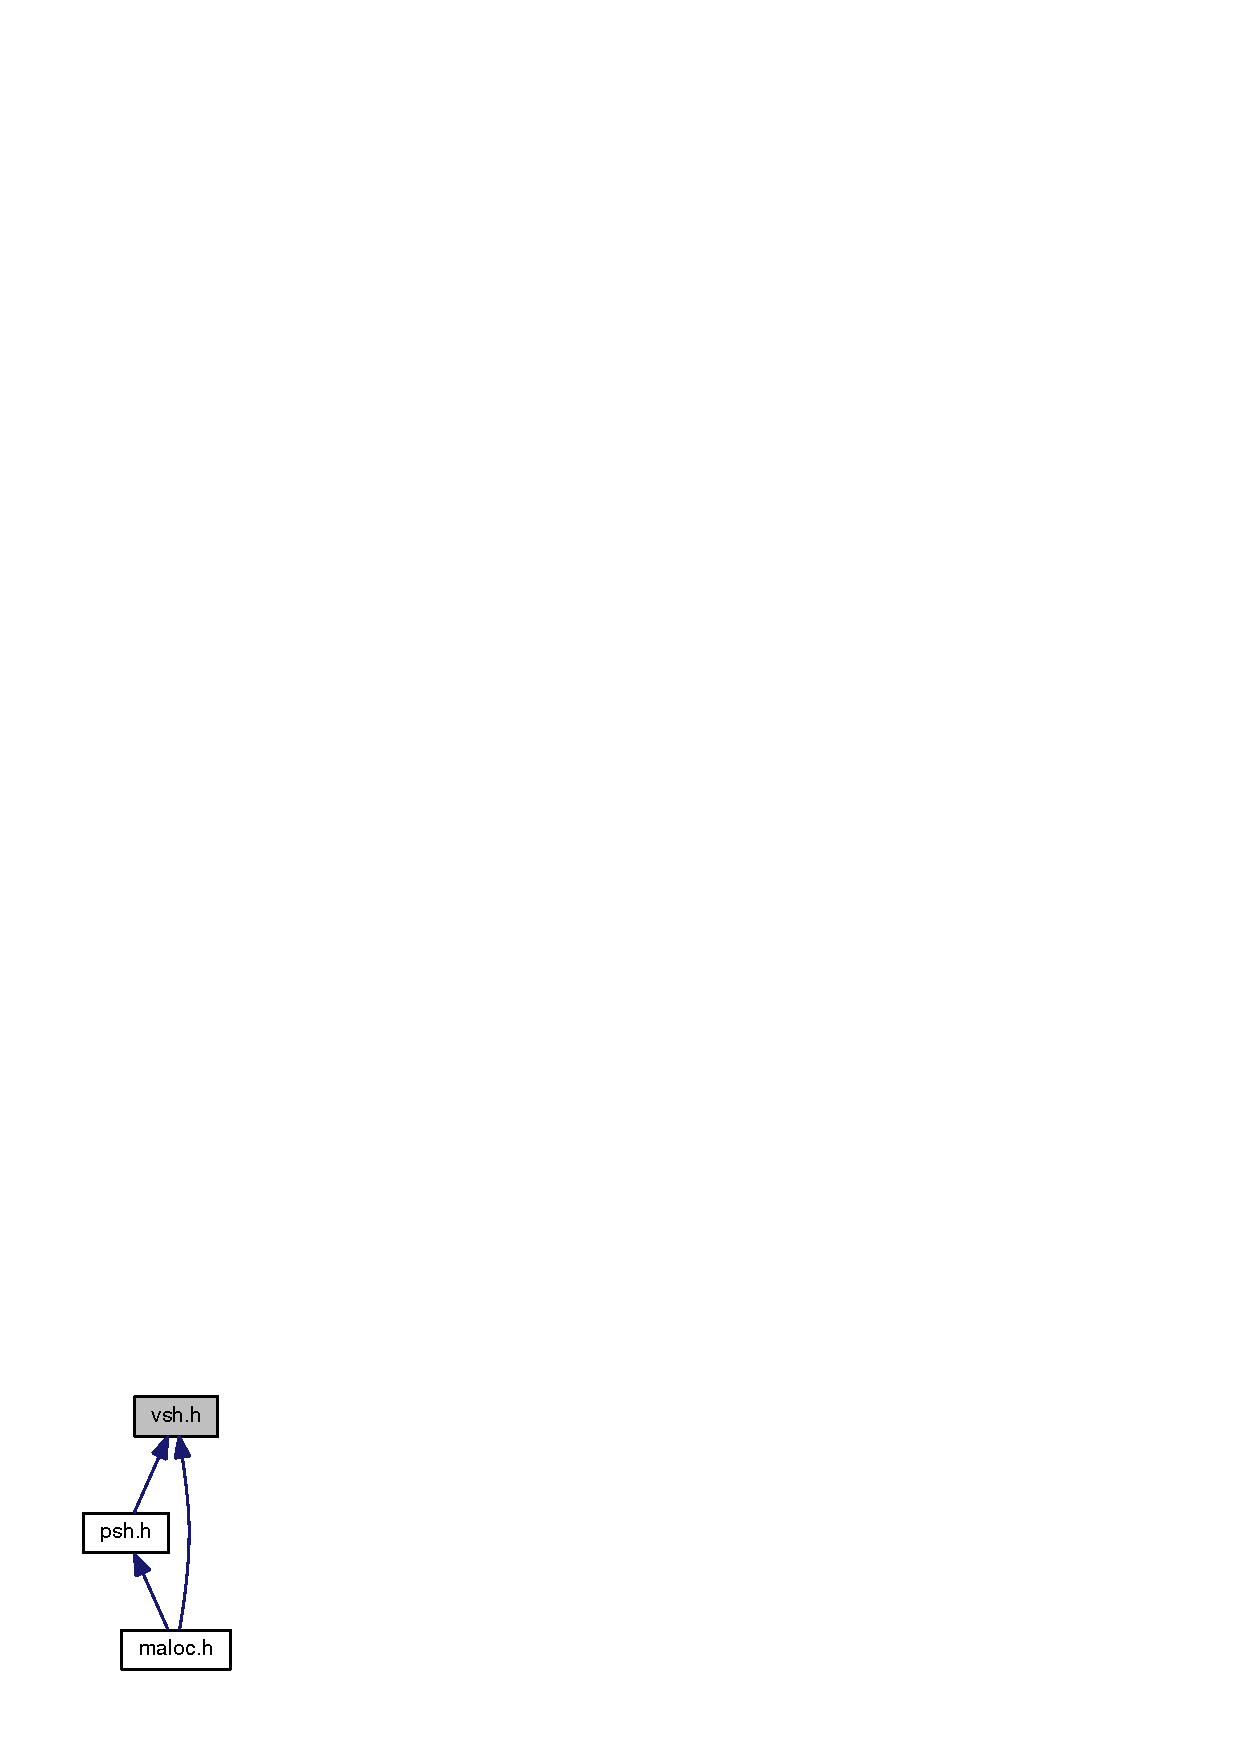
\includegraphics[width=113pt]{a00054}
\end{center}
\end{figure}
\subsection*{Classes}
\begin{DoxyCompactItemize}
\item 
struct {\bf sVsh}
\begin{DoxyCompactList}\small\item\em Contains public data members for Vsh class. \item\end{DoxyCompactList}\end{DoxyCompactItemize}
\subsection*{Typedefs}
\begin{DoxyCompactItemize}
\item 
typedef struct {\bf sVsh} {\bf Vsh}
\begin{DoxyCompactList}\small\item\em Declaration of the Vsh class as the Vsh structure. \item\end{DoxyCompactList}\end{DoxyCompactItemize}
\subsection*{Functions}
\begin{DoxyCompactItemize}
\item 
{\bf Vsh} $\ast$ {\bf Vsh\_\-ctor} ({\bf Vmem} $\ast$vmem, int argc, char $\ast$$\ast$argv)
\begin{DoxyCompactList}\small\item\em Create the shell. \item\end{DoxyCompactList}\item 
void {\bf Vsh\_\-dtor} ({\bf Vsh} $\ast$$\ast$thee)
\begin{DoxyCompactList}\small\item\em Destroy the shell. \item\end{DoxyCompactList}\item 
int {\bf Vsh\_\-shell} ({\bf Vsh} $\ast$thee, char $\ast$pPR, void $\ast$pthee, int($\ast$builtin)(void $\ast$thee, int argc, char $\ast$$\ast$argv))
\begin{DoxyCompactList}\small\item\em A bash-\/like shell with user-\/definable extensions. \item\end{DoxyCompactList}\item 
int {\bf Vsh\_\-putenv} ({\bf Vsh} $\ast$thee, const char $\ast$envi, const char $\ast$valu)
\begin{DoxyCompactList}\small\item\em Place a variable with a value in the environment. \item\end{DoxyCompactList}\item 
int {\bf Vsh\_\-putenvInfo} ({\bf Vsh} $\ast$thee, const char $\ast$envi, const char $\ast$valu)
\begin{DoxyCompactList}\small\item\em Place a variable with an info string in the environment. \item\end{DoxyCompactList}\item 
int {\bf Vsh\_\-putenvInt} ({\bf Vsh} $\ast$thee, const char $\ast$envi, const int valu)
\begin{DoxyCompactList}\small\item\em Place a variable with a value (integer) in the environment. \item\end{DoxyCompactList}\item 
int {\bf Vsh\_\-putenvReal} ({\bf Vsh} $\ast$thee, const char $\ast$envi, const double valu)
\begin{DoxyCompactList}\small\item\em Place a variable with a value (real) in the environment. \item\end{DoxyCompactList}\item 
char $\ast$ {\bf Vsh\_\-getenv} ({\bf Vsh} $\ast$thee, const char $\ast$envi)
\begin{DoxyCompactList}\small\item\em Get a value of variable in the environment. \item\end{DoxyCompactList}\item 
char $\ast$ {\bf Vsh\_\-getenvInfo} ({\bf Vsh} $\ast$thee, const char $\ast$envi)
\begin{DoxyCompactList}\small\item\em Get info associated with a variable in the environment. \item\end{DoxyCompactList}\item 
int {\bf Vsh\_\-getenvInt} ({\bf Vsh} $\ast$thee, const char $\ast$envi)
\begin{DoxyCompactList}\small\item\em Get a value of variable in the environment as an integer. \item\end{DoxyCompactList}\item 
double {\bf Vsh\_\-getenvReal} ({\bf Vsh} $\ast$thee, const char $\ast$envi)
\begin{DoxyCompactList}\small\item\em Get a value of variable in the environment as a real. \item\end{DoxyCompactList}\item 
void {\bf Vsh\_\-remove} ({\bf Vsh} $\ast$thee, const char $\ast$envi)
\begin{DoxyCompactList}\small\item\em Remove a variable from the environment. \item\end{DoxyCompactList}\item 
void {\bf Vsh\_\-wipe} ({\bf Vsh} $\ast$thee)
\begin{DoxyCompactList}\small\item\em Wipe the environment. \item\end{DoxyCompactList}\item 
void {\bf Vsh\_\-memChk} ({\bf Vsh} $\ast$thee)
\begin{DoxyCompactList}\small\item\em Print the exact current malloc usage. \item\end{DoxyCompactList}\item 
{\bf Vio} $\ast$ {\bf Vsh\_\-ioSetup} ({\bf Vsh} $\ast$thee, char $\ast$key)
\begin{DoxyCompactList}\small\item\em Setup for an I/O command. \item\end{DoxyCompactList}\item 
void {\bf Vsh\_\-ioCleanup} ({\bf Vsh} $\ast$thee, {\bf Vio} $\ast$$\ast$sock)
\begin{DoxyCompactList}\small\item\em Cleanup an I/O command. \item\end{DoxyCompactList}\end{DoxyCompactItemize}


\subsection{Detailed Description}
Header file for vsh, a bourne-\/compatible shell. \begin{DoxyAuthor}{Author}
Michael Holst 
\end{DoxyAuthor}
\begin{DoxyNote}{Note}
None 
\end{DoxyNote}
\begin{DoxyVersion}{Version}

\end{DoxyVersion}
\begin{DoxyParagraph}{Id:}
\doxyref{vsh.h}{p.}{a00021},v 1.30 2010/08/12 05:40:29 fetk Exp 
\end{DoxyParagraph}


\begin{DoxyAttention}{Attention}
\begin{DoxyVerb}
 *
 * MALOC = < Minimal Abstraction Layer for Object-oriented C >
 * Copyright (C) 1994-- Michael Holst
 *
 * This library is free software; you can redistribute it and/or
 * modify it under the terms of the GNU Lesser General Public
 * License as published by the Free Software Foundation; either
 * version 2.1 of the License, or (at your option) any later version.
 *
 * This library is distributed in the hope that it will be useful,
 * but WITHOUT ANY WARRANTY; without even the implied warranty of
 * MERCHANTABILITY or FITNESS FOR A PARTICULAR PURPOSE. See the GNU
 * Lesser General Public License for more details.
 *
 * You should have received a copy of the GNU Lesser General Public
 * License along with this library; if not, write to the Free Software
 * Foundation, Inc., 59 Temple Place, Suite 330, Boston, MA 02111-1307 USA
 *
 *  \end{DoxyVerb}
 
\end{DoxyAttention}

\section{vsys.\+h File Reference}
\label{a00022}\index{vsys.\+h@{vsys.\+h}}


The primary header for V\+S\+Y\+S. (Virtual S\+Y\+Stem utilities library.)  


{\ttfamily \#include $<$maloc/maloc\+\_\+base.\+h$>$}\\*
{\ttfamily \#include $<$maloc/vnm.\+h$>$}\\*
{\ttfamily \#include $<$maloc/vmem.\+h$>$}\\*
{\ttfamily \#include $<$maloc/vio.\+h$>$}\\*
{\ttfamily \#include $<$maloc/vset.\+h$>$}\\*
{\ttfamily \#include $<$maloc/vpred.\+h$>$}\\*
Include dependency graph for vsys.\+h\+:\nopagebreak
\begin{figure}[H]
\begin{center}
\leavevmode
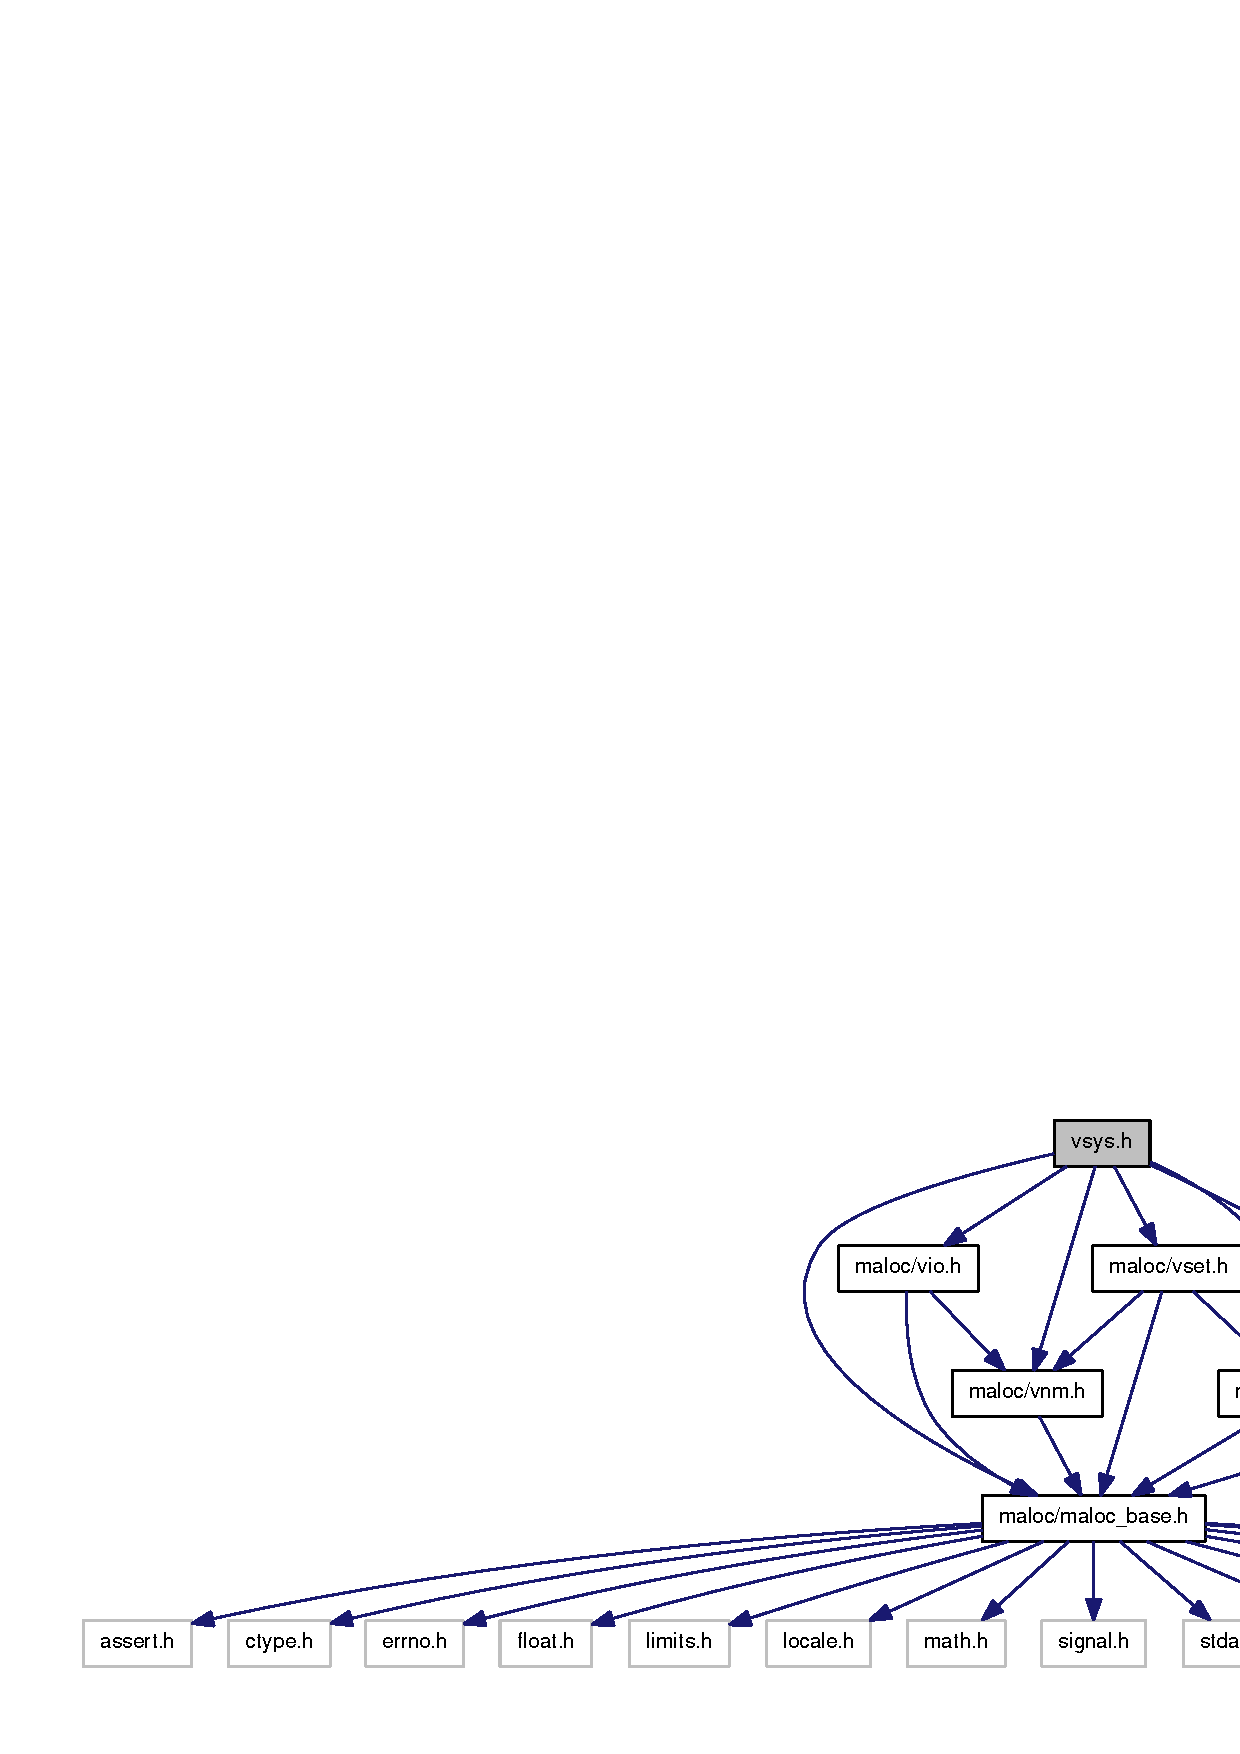
\includegraphics[width=350pt]{a00055}
\end{center}
\end{figure}
This graph shows which files directly or indirectly include this file\+:\nopagebreak
\begin{figure}[H]
\begin{center}
\leavevmode
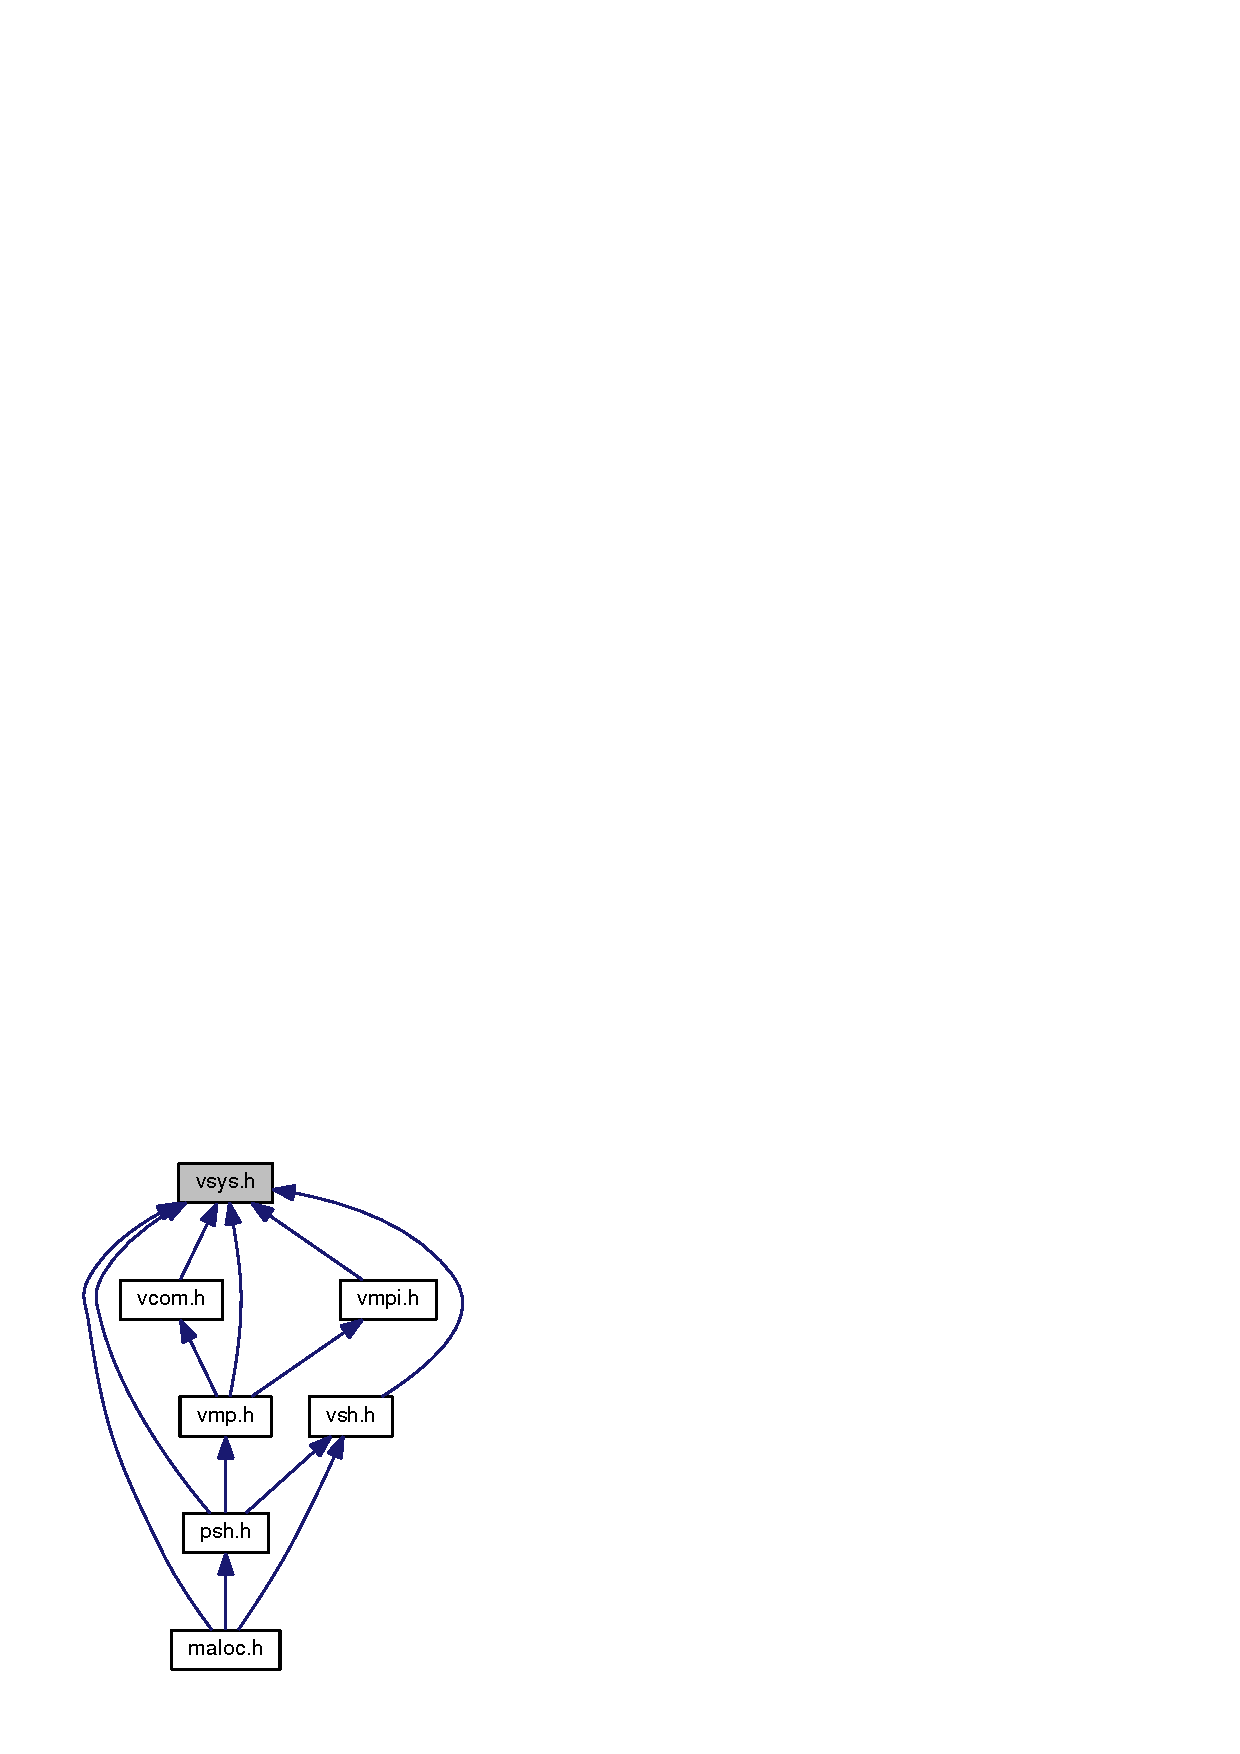
\includegraphics[width=226pt]{a00056}
\end{center}
\end{figure}


\subsection{Detailed Description}
The primary header for V\+S\+Y\+S. (Virtual S\+Y\+Stem utilities library.) 

\begin{DoxyAuthor}{Author}
Michael Holst 
\end{DoxyAuthor}
\begin{DoxyVersion}{Version}

\end{DoxyVersion}
\begin{DoxyParagraph}{Id}
\doxyref{vsys.\+h}{p.}{a00022},v 1.\+12 2010/08/12 05\+:40\+:37 fetk Exp 
\end{DoxyParagraph}


\begin{DoxyAttention}{Attention}
\begin{DoxyVerb}*
* MALOC = < Minimal Abstraction Layer for Object-oriented C >
* Copyright (C) 1994-- Michael Holst
*
* This library is free software; you can redistribute it and/or
* modify it under the terms of the GNU Lesser General Public
* License as published by the Free Software Foundation; either
* version 2.1 of the License, or (at your option) any later version.
*
* This library is distributed in the hope that it will be useful,
* but WITHOUT ANY WARRANTY; without even the implied warranty of
* MERCHANTABILITY or FITNESS FOR A PARTICULAR PURPOSE. See the GNU
* Lesser General Public License for more details.
*
* You should have received a copy of the GNU Lesser General Public
* License along with this library; if not, write to the Free Software
* Foundation, Inc., 59 Temple Place, Suite 330, Boston, MA 02111-1307 USA
* 
*  \end{DoxyVerb}
 
\end{DoxyAttention}

\printindex
\end{document}
